%&preformat-disser
\RequirePackage[l2tabu,orthodox]{nag} % Раскомментировав, можно в логе получать рекомендации относительно правильного использования пакетов и предупреждения об устаревших и нерекомендуемых пакетах
% Формат А4, 14pt (ГОСТ Р 7.0.11-2011, 5.3.6)
\documentclass[a4paper,14pt,oneside,openany,oldfontcommands]{memoir}

%%%%%%%%%%%%%%%%%%%%%%%%%%%%%%%%%%%%%%%%%%%%%%%%%%%%%%%%%%%%%%%%%%%%%%%%%%%%%%%%
%%%% Файл упрощённых настроек шаблона, общих для диссертации и автореферата %%%%
%%%%%%%%%%%%%%%%%%%%%%%%%%%%%%%%%%%%%%%%%%%%%%%%%%%%%%%%%%%%%%%%%%%%%%%%%%%%%%%%

%%% Режим черновика %%%
\makeatletter
\@ifundefined{c@draft}{
  \newcounter{draft}
  \setcounter{draft}{0}  % 0 --- чистовик (максимальное соблюдение ГОСТ)
                         % 1 --- черновик (отклонения от ГОСТ, но быстрая
                         %       сборка итоговых PDF)
}{}
\makeatother

%%% Использование в pdflatex шрифтов не по-умолчанию %%%
\makeatletter
\@ifundefined{c@usealtfont}{
  \newcounter{usealtfont}
  \setcounter{usealtfont}{1}    % 0 --- шрифты на базе Computer Modern
                                % 1 --- использовать пакет pscyr, при его
                                %       наличии
                                % 2 --- использовать пакет XCharter, при наличии
                                %       подходящей версии
}{}
\makeatother

%%% Использование в xelatex и lualatex семейств шрифтов %%%
\makeatletter
\@ifundefined{c@fontfamily}{
  \newcounter{fontfamily}
  \setcounter{fontfamily}{1}  % 0 --- CMU семейство. Используется как fallback;
                              % 1 --- Шрифты от MS (Times New Roman и компания)
                              % 2 --- Семейство Liberation
}{}
\makeatother

%%% Библиография %%%
\makeatletter
\@ifundefined{c@bibliosel}{
  \newcounter{bibliosel}
  \setcounter{bibliosel}{1}   % 0 --- встроенная реализация с загрузкой файла
                              %       через движок bibtex8;
                              % 1 --- реализация пакетом biblatex через движок
                              %       biber
}{}
\makeatother

%%% Предкомпиляция tikz рисунков для ускорения работы %%%
\makeatletter
\@ifundefined{c@imgprecompile}{
  \newcounter{imgprecompile}
  \setcounter{imgprecompile}{0}   % 0 --- без предкомпиляции;
                                  % 1 --- пользоваться предварительно
                                  %       скомпилированными pdf вместо генерации
                                  %       заново из tikz
}{}
\makeatother
            % общие настройки шаблона
%%% Проверка используемого TeX-движка %%%
\newif\ifxetexorluatex   % определяем новый условный оператор (http://tex.stackexchange.com/a/47579)
\ifxetex
    \xetexorluatextrue
\else
    \ifluatex
        \xetexorluatextrue
    \else
        \xetexorluatexfalse
    \fi
\fi

\newif\ifsynopsis           % Условие, проверяющее, что документ --- автореферат

\usepackage{etoolbox}[2015/08/02]               % Для продвинутой проверки разных условий
\providebool{presentation}

%%% Поля и разметка страницы %%%
\usepackage{pdflscape}                              % Для включения альбомных страниц
\usepackage{geometry}                               % Для последующего задания полей

%%% Математические пакеты %%%
\usepackage{amsthm,amsmath,amscd}   % Математические дополнения от AMS
\usepackage{amsfonts,amssymb}       % Математические дополнения от AMS
\usepackage{mathtools}              % Добавляет окружение multlined
\usepackage{xfrac}                  % Красивые дроби
\usepackage[
    locale = DE,
    list-separator       = {;\,},
    list-final-separator = {;\,},
    list-pair-separator  = {;\,},
    range-phrase={\text{\ensuremath{-}}},
    % quotient-mode        = fraction, % красивые дроби могут не соответствовать ГОСТ
    fraction-function    = \sfrac,
    separate-uncertainty,
    ]{siunitx}                      % Размерности SI
\sisetup{inter-unit-product = \ensuremath{{}\cdot{}}}

% Кириллица в нумерации subequations
% Для правильной работы требуется выполнение сразу после загрузки пакетов
\patchcmd{\subequations}{\def\theequation{\theparentequation\alph{equation}}}
{\def\theequation{\theparentequation\asbuk{equation}}}
{\typeout{subequations patched}}{\typeout{subequations not patched}}

%%%% Установки для размера шрифта 14 pt %%%%
%% Формирование переменных и констант для сравнения (один раз для всех подключаемых файлов)%%
%% должно располагаться до вызова пакета fontspec или polyglossia, потому что они сбивают его работу
\newlength{\curtextsize}
\newlength{\bigtextsize}
\setlength{\bigtextsize}{13.9pt}

\makeatletter
%\show\f@size                                       % неплохо для отслеживания, но вызывает стопорение процесса, если документ компилируется без команды  -interaction=nonstopmode
\setlength{\curtextsize}{\f@size pt}
\makeatother

%%% Кодировки и шрифты %%%
\ifxetexorluatex
    \PassOptionsToPackage{no-math}{fontspec}        % https://tex.stackexchange.com/a/26295/104425
    \usepackage{polyglossia}[2014/05/21]            % Поддержка многоязычности (fontspec подгружается автоматически)
\else
   %%% Решение проблемы копирования текста в буфер кракозябрами
    \ifnumequal{\value{usealtfont}}{0}{}{
        \input glyphtounicode.tex
        \input glyphtounicode-cmr.tex %from pdfx package
        \pdfgentounicode=1
    }
    \usepackage{cmap}                               % Улучшенный поиск русских слов в полученном pdf-файле
    \ifnumequal{\value{usealtfont}}{2}{}{
        \defaulthyphenchar=127                      % Если стоит до fontenc, то переносы не впишутся в выделяемый текст при копировании его в буфер обмена
    }
    \usepackage{textcomp}
    \usepackage[T1,T2A]{fontenc}                    % Поддержка русских букв
    \ifnumequal{\value{usealtfont}}{1}{% Используется pscyr, при наличии
        \IfFileExists{pscyr.sty}{\usepackage{pscyr}}{}  % Подключение pscyr
    }{}
    \usepackage[utf8]{inputenc}[2014/04/30]         % Кодировка utf8
    \usepackage[english, russian]{babel}[2014/03/24]% Языки: русский, английский
    \ifnumequal{\value{usealtfont}}{2}{
        % http://dxdy.ru/post1238763.html#p1238763
        \usepackage[scaled=0.960]{XCharter}[2017/12/19] % Подключение русифицированных шрифтов XCharter
        \usepackage[charter, vvarbb, scaled=1.048]{newtxmath}[2017/12/14]
        \ifpresentation
        \else
            \setDisplayskipStretch{-0.078}
        \fi
    }{}
\fi

%%% Оформление абзацев %%%
\usepackage{indentfirst}                            % Красная строка

%%% Цвета %%%
\ifpresentation
\else
    \usepackage[dvipsnames, table, hyperref]{xcolor} % Совместимо с tikz
\fi

%%% Таблицы %%%
\usepackage{longtable,ltcaption} % Длинные таблицы
\usepackage{multirow,makecell}   % Улучшенное форматирование таблиц
\usepackage{tabu, tabulary}      % таблицы с автоматически подбирающейся
                                 % шириной столбцов (tabu обязательно
                                 % до hyperref вызывать)

%%% Общее форматирование
\usepackage{soulutf8}                               % Поддержка переносоустойчивых подчёркиваний и зачёркиваний
\usepackage{icomma}                                 % Запятая в десятичных дробях

%%% Оптимизация расстановки переносов и длины последней строки абзаца
\IfFileExists{impnattypo.sty}{% проверка установленности пакета impnattypo
    \ifluatex
        \ifnumequal{\value{draft}}{1}{% Черновик
            \usepackage[hyphenation, lastparline, nosingleletter, homeoarchy,
            rivers, draft]{impnattypo}
        }{% Чистовик
            \usepackage[hyphenation, lastparline, nosingleletter]{impnattypo}
        }
    \else
        \usepackage[hyphenation, lastparline]{impnattypo}
    \fi
}{}

%% Векторная графика

\usepackage{tikz}                   % Продвинутый пакет векторной графики
\usetikzlibrary{chains}             % Для примера tikz рисунка
\usetikzlibrary{shapes.geometric}   % Для примера tikz рисунка
\usetikzlibrary{shapes.symbols}     % Для примера tikz рисунка
\usetikzlibrary{arrows}             % Для примера tikz рисунка

%%% Гиперссылки %%%
\usepackage{hyperref}[2012/11/06]

%%% Изображения %%%
\usepackage{graphicx}[2014/04/25]                   % Подключаем пакет работы с графикой

%%% Счётчики %%%
\usepackage[figure,table]{totalcount}               % Счётчик рисунков и таблиц
\usepackage{totcount}                               % Пакет создания счётчиков на основе последнего номера подсчитываемого элемента (может требовать дважды компилировать документ)
\usepackage{totpages}                               % Счётчик страниц, совместимый с hyperref (ссылается на номер последней страницы). Желательно ставить последним пакетом в преамбуле

%%% Продвинутое управление групповыми ссылками (пока только формулами) %%%
\ifpresentation
\else
    \usepackage[russian]{cleveref} % cleveref имеет сложности со считыванием
    % языка из babel. Такое решение русификации вывода выбрано вместо
    % определения в documentclass из опасности что-то лишнее передать во все
    % остальные пакеты, включая библиографию.
    \creflabelformat{equation}{#2#1#3} % Формат по умолчанию ставил круглые
    % скобки вокруг каждого номера ссылки, теперь просто номера ссылок без
    % какого-либо дополнительного оформления
    \crefrangelabelformat{equation}{#3#1#4\cyrdash#5#2#6} % Интервалы в русском
    % языке принято делать через тире, если иное не оговорено

    % решение проблемы с "и" в \labelcref
    % https://tex.stackexchange.com/a/455124/104425
    \ifxetexorluatex
        \DeclareTextSymbol{\cyri}\UnicodeEncodingName{"0438} % и
    \fi

    % Добавление возможности использования пробелов в \labelcref
    % https://tex.stackexchange.com/a/340502/104425
    \usepackage{kvsetkeys}
    \makeatletter
    \let\org@@cref\@cref
    \renewcommand*{\@cref}[2]{%
        \edef\process@me{%
            \noexpand\org@@cref{#1}{\zap@space#2 \@empty}%
        }\process@me
    }
    \makeatother

    \newcommand{\eqrefs}[1]{(\labelcref{#1})}
    \newcommand{\refs}[1]{\labelcref{#1}}
\fi

\ifnumequal{\value{draft}}{1}{% Черновик
    \usepackage[firstpage]{draftwatermark}
    \SetWatermarkText{DRAFT}
    \SetWatermarkFontSize{14pt}
    \SetWatermarkScale{15}
    \SetWatermarkAngle{45}
}{}

%%% Исправление положения якорей подписей (под)рисунков %%%
% Без hypcap и патча, при клике по ссылке на подрисунок, просмотрщик pdf прыгает "к подписи" а не "к рисунку".
% Подробнее: https://github.com/AndreyAkinshin/Russian-Phd-LaTeX-Dissertation-Template/issues/238
% (!) Даже с патчем, если мешать в одной фиге разные типы подфиг (subbottom и subcaption) - ссылки всё равно будут работать неправильно  (см. https://www.overleaf.com/read/czmbmmtnqrrg ).
\ifpresentation
\else
    \usepackage[all]{hypcap}

    \makeatletter
    \ltx@ifclasslater{memoir}{2018/12/13}{
        % Предполагается, что в следующей версии класс будет исправлен
        \typeout{Assuming this version of memoir is free from the jumping-to-caption bug.}
    }{
        \usepackage{xpatch}

        \newcommand\mem@step@subcounter{\refstepcounter{sub\@captype}\@contkeep}

        \xpatchcmd{\@memsubbody}%
        {\refstepcounter{sub\@captype}\@contkeep}% search pattern
        {}% replacement
        {\typeout{@memsubbody is patched}}%
        {\typeout{@memsubbody is NOT patched}}%

        \xpatchcmd{\@memcontsubbody}%
        {\refstepcounter{sub\@captype}\@contkeep}% pattern
        {}% replacement
        {\typeout{@memcontsubbody is patched}}%
        {\typeout{@memcontsubbody is NOT patched}}%

        \xpatchcmd{\@memsubfloat}%
        {\vbox\bgroup}% search pattern
        {\vbox\bgroup\mem@step@subcounter}% replacement
        {\typeout{@memsubfloat patch is ok}}%
        {\typeout{@memsubfloat patch is NOT ok}}%

        \xpatchcmd{\subcaption}%
        {\refstepcounter{sub\@captype}}% search pattern
        {\H@refstepcounter{sub\@captype}}% replacement
        {\typeout{subcaption second patch is ok}}%
        {\typeout{subcaption second patch is NOT ok}}%
    }
    \makeatother
\fi

%%% Цитата, не приводимая в автореферате:
% возможно, актуальна только для biblatex
%\newcommand{\citeinsynopsis}[1]{\ifsynopsis\else ~\cite{#1} \fi}

% если текущий процесс запущен библиотекой tikz-external, то прекомпиляция должна быть включена
\ifdefined\tikzexternalrealjob
    \setcounter{imgprecompile}{1}
\fi

\ifnumequal{\value{imgprecompile}}{1}{% Только если у нас включена предкомпиляция
    \usetikzlibrary{external}   % подключение возможности предкомпиляции
    \tikzexternalize[prefix=images/cache/] % activate! % здесь можно указать отдельную папку для скомпилированных файлов
    \ifxetex
        \tikzset{external/up to date check={diff}}
    \fi
}{}
\usepackage{euscript}         % Пакеты общие для диссертации и автореферата
\synopsisfalse                      % Этот документ --- не автореферат 
%%% Прикладные пакеты %%%
%\usepackage{calc}               % Пакет для расчётов параметров, например длины

%%% Для добавления Стр. над номерами страниц в оглавлении
%%% http://tex.stackexchange.com/a/306950
\usepackage{afterpage}

%%% Списки %%%
\usepackage{enumitem}
    % Пакеты для диссертации
\usepackage{fr-longtable}    %ради \endlasthead

% Листинги с исходным кодом программ
\usepackage{fancyvrb}
\usepackage{listings}
\lccode`\~=0\relax %Без этого хака из-за особенностей пакета listings перестают работать конструкции с \MakeLowercase и т. п. в (xe|lua)latex

% Русская традиция начертания греческих букв
\usepackage{upgreek} % прямые греческие ради русской традиции
\usepackage{xcolor}
\usepackage{cases}
\usepackage{empheq}
%%% Микротипографика
%\ifnumequal{\value{draft}}{0}{% Только если у нас режим чистовика
%    \usepackage[final, babel, shrink=45]{microtype}[2016/05/14] % улучшает представление букв и слов в строках, может помочь при наличии отдельно висящих слов
%}{}

% Отметка о версии черновика на каждой странице
% Чтобы работало надо в своей локальной копии по инструкции
% https://www.ctan.org/pkg/gitinfo2 создать небходимые файлы в папке
% ./git/hooks
% If you’re familiar with tweaking git, you can probably work it out for
% yourself. If not, I suggest you follow these steps:
% 1. First, you need a git repository and working tree. For this example,
% let’s suppose that the root of the working tree is in ~/compsci
% 2. Copy the file post-xxx-sample.txt (which is in the same folder of
% your TEX distribution as this pdf) into the git hooks directory in your
% working copy. In our example case, you should end up with a file called
% ~/compsci/.git/hooks/post-checkout
% 3. If you’re using a unix-like system, don’t forget to make the file executable.
% Just how you do this is outside the scope of this manual, but one
% possible way is with commands such as this:
% chmod g+x post-checkout.
% 4. Test your setup with “git checkout master” (or another suitable branch
% name). This should generate copies of gitHeadInfo.gin in the directories
% you intended.
% 5. Now make two more copies of this file in the same directory (hooks),
% calling them post-commit and post-merge, and you’re done. As before,
% users of unix-like systems should ensure these files are marked as
% executable.
\ifnumequal{\value{draft}}{1}{% Черновик
   \IfFileExists{.git/gitHeadInfo.gin}{
      \usepackage[mark,pcount]{gitinfo2}
      \renewcommand{\gitMark}{rev.\gitAbbrevHash\quad\gitCommitterEmail\quad\gitAuthorIsoDate}
      \renewcommand{\gitMarkFormat}{\rmfamily\color{Gray}\small\bfseries}
   }{}
}{}   % Пакеты для специфических пользовательских задач

%%%%%%%%%%%%%%%%%%%%%%%%%%%%%%%%%%%%%%%%%%%%%%%%%%%%%%
%%%% Файл упрощённых настроек шаблона диссертации %%%%
%%%%%%%%%%%%%%%%%%%%%%%%%%%%%%%%%%%%%%%%%%%%%%%%%%%%%%

%%% Инициализирование переменных, не трогать!  %%%
\newcounter{intvl}
\newcounter{otstup}
\newcounter{contnumeq}
\newcounter{contnumfig}
\newcounter{contnumtab}
\newcounter{pgnum}
\newcounter{chapstyle}
\newcounter{headingdelim}
\newcounter{headingalign}
\newcounter{headingsize}
\newcounter{tabcap}
\newcounter{tablaba}
\newcounter{tabtita}
%%%%%%%%%%%%%%%%%%%%%%%%%%%%%%%%%%%%%%%%%%%%%%%%%%%%%%

%%% Область упрощённого управления оформлением %%%

%% Интервал между заголовками и между заголовком и текстом %%
% Заголовки отделяют от текста сверху и снизу
% тремя интервалами (ГОСТ Р 7.0.11-2011, 5.3.5)
\setcounter{intvl}{3}               % Коэффициент кратности к размеру шрифта

%% Отступы у заголовков в тексте %%
\setcounter{otstup}{0}              % 0 --- без отступа; 1 --- абзацный отступ

%% Нумерация формул, таблиц и рисунков %%
% Нумерация формул
\setcounter{contnumeq}{0}   % 0 --- пораздельно (во введении подряд,
                            %       без номера раздела);
                            % 1 --- сквозная нумерация по всей диссертации
% Нумерация рисунков
\setcounter{contnumfig}{0}  % 0 --- пораздельно (во введении подряд,
                            %       без номера раздела);
                            % 1 --- сквозная нумерация по всей диссертации
% Нумерация таблиц
\setcounter{contnumtab}{1}  % 0 --- пораздельно (во введении подряд,
                            %       без номера раздела);
                            % 1 --- сквозная нумерация по всей диссертации

%% Оглавление %%
\setcounter{pgnum}{1}       % 0 --- номера страниц никак не обозначены;
                            % 1 --- Стр. над номерами страниц (дважды
                            %       компилировать после изменения настройки)
\settocdepth{subsection}    % до какого уровня подразделов выносить в оглавление
\setsecnumdepth{subsection} % до какого уровня нумеровать подразделы


%% Текст и форматирование заголовков %%
\setcounter{chapstyle}{1}     % 0 --- разделы только под номером;
                              % 1 --- разделы с названием "Глава" перед номером
\setcounter{headingdelim}{1}  % 0 --- номер отделен пропуском в 1em или \quad;
                              % 1 --- номера разделов и приложений отделены
                              %       точкой с пробелом, подразделы пропуском
                              %       без точки;
                              % 2 --- номера разделов, подразделов и приложений
                              %       отделены точкой с пробелом.

%% Выравнивание заголовков в тексте %%
\setcounter{headingalign}{0}  % 0 --- по центру;
                              % 1 --- по левому краю

%% Размеры заголовков в тексте %%
\setcounter{headingsize}{0}   % 0 --- по ГОСТ, все всегда 14 пт;
                              % 1 --- пропорционально изменяющийся размер
                              %       в зависимости от базового шрифта

%% Подпись таблиц %%
\setcounter{tabcap}{0}  % 0 --- по ГОСТ, номер таблицы и название разделены
                        %       тире, выровнены по левому краю, при
                        %       необходимостина нескольких строках;
                        % 1 --- подпись таблицы не по ГОСТ, на двух и более
                        %       строках, дальнейшие настройки:
%Выравнивание первой строки, с подписью и номером
\setcounter{tablaba}{2} % 0 --- по левому краю;
                        % 1 --- по центру;
                        % 2 --- по правому краю
%Выравнивание строк с самим названием таблицы
\setcounter{tabtita}{1} % 0 --- по левому краю;
                        % 1 --- по центру;
                        % 2 --- по правому краю
%Разделитель записи «Таблица #» и названия таблицы
\newcommand{\tablabelsep}{ }

%% Подпись рисунков %%
%Разделитель записи «Рисунок #» и названия рисунка
\newcommand{\figlabelsep}{~\cyrdash\ }  % (ГОСТ 2.105, 4.3.1)
                                        % "--- здесь не работает

%%% Цвета гиперссылок %%%
% Latex color definitions: http://latexcolor.com/
\definecolor{linkcolor}{rgb}{0.9,0,0}
\definecolor{citecolor}{rgb}{0,0.6,0}
\definecolor{urlcolor}{rgb}{0,0,1}
%\definecolor{linkcolor}{rgb}{0,0,0} %black
%\definecolor{citecolor}{rgb}{0,0,0} %black
%\definecolor{urlcolor}{rgb}{0,0,0} %black
      % Упрощённые настройки шаблона

% Новые переменные, которые могут использоваться во всём проекте
% ГОСТ 7.0.11-2011
% 9.2 Оформление текста автореферата диссертации
% 9.2.1 Общая характеристика работы включает в себя следующие основные структурные
% элементы:
% актуальность темы исследования;
\newcommand{\actualityTXT}{Актуальность темы.}
% степень ее разработанности;
\newcommand{\progressTXT}{Степень разработанности темы.}
% цели и задачи;
\newcommand{\aimTXT}{Целью}
\newcommand{\tasksTXT}{задачи}
% научную новизну;
\newcommand{\noveltyTXT}{Научная новизна:}
% теоретическую и практическую значимость работы;
%\newcommand{\influenceTXT}{Теоретическая и практическая значимость}
% или чаще используют просто
\newcommand{\influenceTXT}{Практическая значимость}
% методологию и методы исследования;
\newcommand{\methodsTXT}{Методология и методы исследования.}
% положения, выносимые на защиту;
\newcommand{\defpositionsTXT}{Основные положения, выносимые на~защиту:}
% степень достоверности и апробацию результатов.
\newcommand{\reliabilityTXT}{Достоверность}
\newcommand{\probationTXT}{Апробация работы.}

\newcommand{\contributionTXT}{Личный вклад.}
\newcommand{\publicationsTXT}{Публикации.}


%%% Заголовки библиографии:

% для автореферата:
\newcommand{\bibtitleauthor}{Публикации автора по теме диссертации}

% для стиля библиографии `\insertbiblioauthorgrouped`
\newcommand{\bibtitleauthorvak}{В изданиях из списка ВАК РФ}
\newcommand{\bibtitleauthorscopus}{В изданиях, входящих в международную базу цитирования Scopus}
\newcommand{\bibtitleauthorwos}{В изданиях, входящих в международную базу цитирования Web of Science}
\newcommand{\bibtitleauthorother}{В прочих изданиях}
\newcommand{\bibtitleauthorconf}{В сборниках трудов конференций}

% для стиля библиографии `\insertbiblioauthorimportant`:
\newcommand{\bibtitleauthorimportant}{Наиболее значимые \protect\MakeLowercase\bibtitleauthor}

% для списка литературы в диссертации и списка чужих работ в автореферате:
\newcommand{\bibtitlefull}{Список литературы} % (ГОСТ Р 7.0.11-2011, 4)

%Наши переобозначения
\def \q {{\bf q}}
\def \br {{\bf r}}
\def \k {{\bf k}}
\def \n {{\bf n}}
\def \ve {\varepsilon}         % Новые переменные, для всего проекта

%%% Основные сведения %%%
\newcommand{\thesisAuthorLastName}{{Оскирко}}
\newcommand{\thesisAuthorOtherNames}{{Антон Дмитриевич}}
\newcommand{\thesisAuthorInitials}{{А.\,Д.}}
\newcommand{\thesisAuthor}             % Диссертация, ФИО автора
{%
    \texorpdfstring{% \texorpdfstring takes two arguments and uses the first for (La)TeX and the second for pdf
        \thesisAuthorLastName~\thesisAuthorOtherNames% так будет отображаться на титульном листе или в тексте, где будет использоваться переменная
    }{%
        \thesisAuthorLastName, \thesisAuthorOtherNames% эта запись для свойств pdf-файла. В таком виде, если pdf будет обработан программами для сбора библиографических сведений, будет правильно представлена фамилия.
    }
}
\newcommand{\thesisAuthorShort}        % Диссертация, ФИО автора инициалами
{\thesisAuthorInitials~\thesisAuthorLastName}
%\newcommand{\thesisUdk}                % Диссертация, УДК
%{\todo{xxx.xxx}}
\newcommand{\finishWork}
{Выпускная квалификационная работа}
\newcommand{\thesisTitle}              % Диссертация, название
{Исследование изменения ориентационной структуры кирального жидкого кристалла с~большим флексоэлектрическим коэффициентом под~воздействием внешнего электрического поля}
\newcommand{\thesisSpecialtyNumber}    % Диссертация, специальность, номер
{\todo{01.04.02}}
\newcommand{\thesisSpecialtyTitle}     % Диссертация, специальность, название (название взято с сайта ВАК для примера)
{\todo{Теоретическая~физика}}
%% \newcommand{\thesisSpecialtyTwoNumber} % Диссертация, вторая специальность, номер
%% {\todo{XX.XX.XX}}
%% \newcommand{\thesisSpecialtyTwoTitle}  % Диссертация, вторая специальность, название
%% {\todo{Теория и~методика физического воспитания, спортивной тренировки,
%% оздоровительной и~адаптивной физической культуры}}
\newcommand{\thesisDegree}             % Диссертация, ученая степень
{{кандидата физико-математических наук}}
\newcommand{\thesisDegreeShort}        % Диссертация, ученая степень, краткая запись
{\todo{канд. физ.-мат. наук}}
\newcommand{\thesisCity}               % Диссертация, город написания диссертации
{{Санкт-Петербург}}
\newcommand{\thesisYear}               % Диссертация, год написания диссертации
{{2020}}
\newcommand{\thesisOrganization}       % Диссертация, организация
{Санкт-Петербургский Государственный Университет}
\newcommand{\thesisOrganizationShort}  % Диссертация, краткое название организации для доклада
{\todo{СПбГУ}}

\newcommand{\thesisInOrganization}     % Диссертация, организация в предложном падеже: Работа выполнена в ...
{\todo{Санкт-Петербургский Государственный Университет}}

%% \newcommand{\supervisorDead}{}           % Рисовать рамку вокруг фамилии
\newcommand{\supervisorFio}              % Научный руководитель, ФИО
{{Ульянов Сергей Владимирович}}
\newcommand{\supervisorRegalia}          % Научный руководитель, регалии
{{доктор физико-математических наук, профессор}}
\newcommand{\supervisorFioShort}         % Научный руководитель, ФИО
{\todo{С.\,В.~Ульянов}}
\newcommand{\supervisorRegaliaShort}     % Научный руководитель, регалии
{\todo{д.~ф.-м.~н.,~проф.}}

%% \newcommand{\supervisorTwoDead}{}        % Рисовать рамку вокруг фамилии
%% \newcommand{\supervisorTwoFio}           % Второй научный руководитель, ФИО
%% {\todo{Фамилия Имя Отчество}}
%% \newcommand{\supervisorTwoRegalia}       % Второй научный руководитель, регалии
%% {\todo{уч. степень, уч. звание}}
%% \newcommand{\supervisorTwoFioShort}      % Второй научный руководитель, ФИО
%% {\todo{И.\,О.~Фамилия}}
%% \newcommand{\supervisorTwoRegaliaShort}  % Второй научный руководитель, регалии
%% {\todo{уч.~ст.,~уч.~зв.}}

\newcommand{\opponentOneFio}           % Оппонент 1, ФИО
{\todo{Фамилия Имя Отчество}}
\newcommand{\opponentOneRegalia}       % Оппонент 1, регалии
{\todo{доктор физико-математических наук, профессор}}
\newcommand{\opponentOneJobPlace}      % Оппонент 1, место работы
{\todo{Не очень длинное название для места работы}}
\newcommand{\opponentOneJobPost}       % Оппонент 1, должность
{\todo{старший научный сотрудник}}

\newcommand{\opponentTwoFio}           % Оппонент 2, ФИО
{\todo{Фамилия Имя Отчество}}
\newcommand{\opponentTwoRegalia}       % Оппонент 2, регалии
{\todo{кандидат физико-математических наук}}
\newcommand{\opponentTwoJobPlace}      % Оппонент 2, место работы
{\todo{Основное место работы c длинным длинным длинным длинным названием}}
\newcommand{\opponentTwoJobPost}       % Оппонент 2, должность
{\todo{старший научный сотрудник}}

%% \newcommand{\opponentThreeFio}         % Оппонент 3, ФИО
%% {\todo{Фамилия Имя Отчество}}
%% \newcommand{\opponentThreeRegalia}     % Оппонент 3, регалии
%% {\todo{кандидат физико-математических наук}}
%% \newcommand{\opponentThreeJobPlace}    % Оппонент 3, место работы
%% {\todo{Основное место работы c длинным длинным длинным длинным названием}}
%% \newcommand{\opponentThreeJobPost}     % Оппонент 3, должность
%% {\todo{старший научный сотрудник}}

\newcommand{\leadingOrganizationTitle} % Ведущая организация, дополнительные строки. Удалить, чтобы не отображать в автореферате
{\todo{Федеральное государственное бюджетное образовательное учреждение высшего
профессионального образования с~длинным длинным длинным длинным названием}}

\newcommand{\defenseDate}              % Защита, дата
{\todo{DD mmmmmmmm YYYY~г.~в~XX часов}}
\newcommand{\defenseCouncilNumber}     % Защита, номер диссертационного совета
{\todo{Д\,123.456.78}}
\newcommand{\defenseCouncilTitle}      % Защита, учреждение диссертационного совета
{\todo{Название учреждения}}
\newcommand{\defenseCouncilAddress}    % Защита, адрес учреждение диссертационного совета
{\todo{Адрес}}
\newcommand{\defenseCouncilPhone}      % Телефон для справок
{\todo{+7~(0000)~00-00-00}}

\newcommand{\defenseSecretaryFio}      % Секретарь диссертационного совета, ФИО
{\todo{Фамилия Имя Отчество}}
\newcommand{\defenseSecretaryRegalia}  % Секретарь диссертационного совета, регалии
{\todo{д-р~физ.-мат. наук}}            % Для сокращений есть ГОСТы, например: ГОСТ Р 7.0.12-2011 + http://base.garant.ru/179724/#block_30000

\newcommand{\synopsisLibrary}          % Автореферат, название библиотеки
{\todo{Название библиотеки}}
\newcommand{\synopsisDate}             % Автореферат, дата рассылки
{\todo{DD mmmmmmmm YYYY года}}

% To avoid conflict with beamer class use \providecommand
\providecommand{\keywords}%            % Ключевые слова для метаданных PDF диссертации и автореферата
{}
             % Основные сведения
%%% Кодировки и шрифты %%%
\ifxetexorluatex
    \setmainlanguage[babelshorthands=true]{russian}    % Язык по-умолчанию русский с поддержкой приятных команд пакета babel
    \setotherlanguage{english}                         % Дополнительный язык = английский (в американской вариации по-умолчанию)

    % Проверка существования шрифтов. Недоступна в pdflatex
    \ifnumequal{\value{fontfamily}}{1}{
        \IfFontExistsTF{Times New Roman}{}{\setcounter{fontfamily}{0}}
    }{}
    \ifnumequal{\value{fontfamily}}{2}{
        \IfFontExistsTF{LiberationSerif}{}{\setcounter{fontfamily}{0}}
    }{}

    \ifnumequal{\value{fontfamily}}{0}{                    % Семейство шрифтов CMU. Используется как fallback
        \setmonofont{CMU Typewriter Text}                  % моноширинный шрифт
        \newfontfamily\cyrillicfonttt{CMU Typewriter Text} % моноширинный шрифт для кириллицы
        \defaultfontfeatures{Ligatures=TeX}                % стандартные лигатуры TeX, замены нескольких дефисов на тире и т. п. Настройки моноширинного шрифта должны идти до этой строки, чтобы при врезках кода программ в коде не применялись лигатуры и замены дефисов
        \setmainfont{CMU Serif}                            % Шрифт с засечками
        \newfontfamily\cyrillicfont{CMU Serif}             % Шрифт с засечками для кириллицы
        \setsansfont{CMU Sans Serif}                       % Шрифт без засечек
        \newfontfamily\cyrillicfontsf{CMU Sans Serif}      % Шрифт без засечек для кириллицы
    }

    \ifnumequal{\value{fontfamily}}{1}{                    % Семейство MS шрифтов
        \setmonofont{Courier New}                          % моноширинный шрифт
        \newfontfamily\cyrillicfonttt{Courier New}         % моноширинный шрифт для кириллицы
        \defaultfontfeatures{Ligatures=TeX}                % стандартные лигатуры TeX, замены нескольких дефисов на тире и т. п. Настройки моноширинного шрифта должны идти до этой строки, чтобы при врезках кода программ в коде не применялись лигатуры и замены дефисов
        \setmainfont{Times New Roman}                      % Шрифт с засечками
        \newfontfamily\cyrillicfont{Times New Roman}       % Шрифт с засечками для кириллицы
        \setsansfont{Arial}                                % Шрифт без засечек
        \newfontfamily\cyrillicfontsf{Arial}               % Шрифт без засечек для кириллицы
    }

    \ifnumequal{\value{fontfamily}}{2}{                    % Семейство шрифтов Liberation (https://pagure.io/liberation-fonts)
        \setmonofont{LiberationMono}[Scale=0.87] % моноширинный шрифт
        \newfontfamily\cyrillicfonttt{LiberationMono}[     % моноширинный шрифт для кириллицы
            Scale=0.87]
        \defaultfontfeatures{Ligatures=TeX}                % стандартные лигатуры TeX, замены нескольких дефисов на тире и т. п. Настройки моноширинного шрифта должны идти до этой строки, чтобы при врезках кода программ в коде не применялись лигатуры и замены дефисов
        \setmainfont{LiberationSerif}                      % Шрифт с засечками
        \newfontfamily\cyrillicfont{LiberationSerif}       % Шрифт с засечками для кириллицы
        \setsansfont{LiberationSans}                       % Шрифт без засечек
        \newfontfamily\cyrillicfontsf{LiberationSans}      % Шрифт без засечек для кириллицы
    }

\else
    \ifnumequal{\value{usealtfont}}{1}{% Используется pscyr, при наличии
        \IfFileExists{pscyr.sty}{\renewcommand{\rmdefault}{ftm}}{}
    }{}
\fi
            % Определение шрифтов (частичное)
%%% Шаблон %%%
\DeclareRobustCommand{\todo}{\textcolor{red}}       % решаем проблему превращения названия цвета в результате \MakeUppercase, http://tex.stackexchange.com/a/187930, \DeclareRobustCommand protects \todo from expanding inside \MakeUppercase
\AtBeginDocument{%
    \setlength{\parindent}{2.5em}                   % Абзацный отступ. Должен быть одинаковым по всему тексту и равен пяти знакам (ГОСТ Р 7.0.11-2011, 5.3.7).
}

%%% Подписи %%%
\setlength{\abovecaptionskip}{0pt}   % Отбивка над подписью
\setlength{\belowcaptionskip}{0pt}   % Отбивка под подписью
\captionwidth{\linewidth}
\normalcaptionwidth

%%% Таблицы %%%
\ifnumequal{\value{tabcap}}{0}{%
    \newcommand{\tabcapalign}{\raggedright}  % по левому краю страницы или аналога parbox
    \renewcommand{\tablabelsep}{~\cyrdash\ } % тире как разделитель идентификатора с номером от наименования
    \newcommand{\tabtitalign}{}
}{%
    \ifnumequal{\value{tablaba}}{0}{%
        \newcommand{\tabcapalign}{\raggedright}  % по левому краю страницы или аналога parbox
    }{}

    \ifnumequal{\value{tablaba}}{1}{%
        \newcommand{\tabcapalign}{\centering}    % по центру страницы или аналога parbox
    }{}

    \ifnumequal{\value{tablaba}}{2}{%
        \newcommand{\tabcapalign}{\raggedleft}   % по правому краю страницы или аналога parbox
    }{}

    \ifnumequal{\value{tabtita}}{0}{%
        \newcommand{\tabtitalign}{\par\raggedright}  % по левому краю страницы или аналога parbox
    }{}

    \ifnumequal{\value{tabtita}}{1}{%
        \newcommand{\tabtitalign}{\par\centering}    % по центру страницы или аналога parbox
    }{}

    \ifnumequal{\value{tabtita}}{2}{%
        \newcommand{\tabtitalign}{\par\raggedleft}   % по правому краю страницы или аналога parbox
    }{}
}

\precaption{\tabcapalign} % всегда идет перед подписью или \legend
\captionnamefont{\normalfont\normalsize} % Шрифт надписи «Таблица #»; также определяет шрифт у \legend
\captiondelim{\tablabelsep} % разделитель идентификатора с номером от наименования
\captionstyle[\tabtitalign]{\tabtitalign}
\captiontitlefont{\normalfont\normalsize} % Шрифт с текстом подписи

%%% Рисунки %%%
\setfloatadjustment{figure}{%
    \setlength{\abovecaptionskip}{0pt}   % Отбивка над подписью
    \setlength{\belowcaptionskip}{0pt}   % Отбивка под подписью
    \precaption{} % всегда идет перед подписью или \legend
    \captionnamefont{\normalfont\normalsize} % Шрифт надписи «Рисунок #»; также определяет шрифт у \legend
    \captiondelim{\figlabelsep} % разделитель идентификатора с номером от наименования
    \captionstyle[\centering]{\centering} % Центрирование подписей, заданных командой \caption и \legend
    \captiontitlefont{\normalfont\normalsize} % Шрифт с текстом подписи
    \postcaption{} % всегда идет после подписи или \legend, и с новой строки
}

%%% Подписи подрисунков %%%
\newsubfloat{figure} % Включает возможность использовать подрисунки у окружений figure
\renewcommand{\thesubfigure}{\asbuk{subfigure}}           % Буквенные номера подрисунков
\subcaptionsize{\normalsize} % Шрифт подписи названий подрисунков (не отличается от основного)
\subcaptionlabelfont{\normalfont}
\subcaptionfont{\!\!) \normalfont} % Вот так тут добавили скобку после буквы.
\subcaptionstyle{\centering}
%\subcaptionsize{\fontsize{12pt}{13pt}\selectfont} % объявляем шрифт 12pt для использования в подписях, тут же надо интерлиньяж объявлять, если не наследуется

%%% Настройки гиперссылок %%%
\ifluatex
    \hypersetup{
        unicode,                % Unicode encoded PDF strings
    }
\fi

\hypersetup{
    linktocpage=true,           % ссылки с номера страницы в оглавлении, списке таблиц и списке рисунков
%    linktoc=all,                % both the section and page part are links
%    pdfpagelabels=false,        % set PDF page labels (true|false)
    plainpages=false,           % Forces page anchors to be named by the Arabic form  of the page number, rather than the formatted form
    colorlinks,                 % ссылки отображаются раскрашенным текстом, а не раскрашенным прямоугольником, вокруг текста
    linkcolor={linkcolor},      % цвет ссылок типа ref, eqref и подобных
    citecolor={citecolor},      % цвет ссылок-цитат
    urlcolor={urlcolor},        % цвет гиперссылок
%    hidelinks,                  % Hide links (removing color and border)
    pdftitle={\thesisTitle},    % Заголовок
    pdfauthor={\thesisAuthor},  % Автор
    pdfsubject={\thesisSpecialtyNumber\ \thesisSpecialtyTitle},      % Тема
%    pdfcreator={Создатель},     % Создатель, Приложение
%    pdfproducer={Производитель},% Производитель, Производитель PDF
    pdfkeywords={\keywords},    % Ключевые слова
    pdflang={ru},
}
\ifnumequal{\value{draft}}{1}{% Черновик
    \hypersetup{
        draft,
    }
}{}

%%% Списки %%%
% Используем короткое тире (endash) для ненумерованных списков (ГОСТ 2.105-95, пункт 4.1.7, требует дефиса, но так лучше смотрится)
\renewcommand{\labelitemi}{\normalfont\bfseries{--}}

% Перечисление строчными буквами латинского алфавита (ГОСТ 2.105-95, 4.1.7)
%\renewcommand{\theenumi}{\alph{enumi}}
%\renewcommand{\labelenumi}{\theenumi)}

% Перечисление строчными буквами русского алфавита (ГОСТ 2.105-95, 4.1.7)
\makeatletter
\AddEnumerateCounter{\asbuk}{\russian@alph}{щ}      % Управляем списками/перечислениями через пакет enumitem, а он 'не знает' про asbuk, потому 'учим' его
\makeatother
%\renewcommand{\theenumi}{\asbuk{enumi}} %первый уровень нумерации
%\renewcommand{\labelenumi}{\theenumi)} %первый уровень нумерации
\renewcommand{\theenumii}{\asbuk{enumii}} %второй уровень нумерации
\renewcommand{\labelenumii}{\theenumii)} %второй уровень нумерации
\renewcommand{\theenumiii}{\arabic{enumiii}} %третий уровень нумерации
\renewcommand{\labelenumiii}{\theenumiii)} %третий уровень нумерации

\setlist{nosep,%                                    % Единый стиль для всех списков (пакет enumitem), без дополнительных интервалов.
    labelindent=\parindent,leftmargin=*%            % Каждый пункт, подпункт и перечисление записывают с абзацного отступа (ГОСТ 2.105-95, 4.1.8)
}

%%% Правильная нумерация приложений, рисунков и формул %%%
%% По ГОСТ 2.105, п. 4.3.8 Приложения обозначают заглавными буквами русского алфавита,
%% начиная с А, за исключением букв Ё, З, Й, О, Ч, Ь, Ы, Ъ.
%% Здесь также переделаны все нумерации русскими буквами.
\ifxetexorluatex
    \makeatletter
    \def\russian@Alph#1{\ifcase#1\or
       А\or Б\or В\or Г\or Д\or Е\or Ж\or
       И\or К\or Л\or М\or Н\or
       П\or Р\or С\or Т\or У\or Ф\or Х\or
       Ц\or Ш\or Щ\or Э\or Ю\or Я\else\xpg@ill@value{#1}{russian@Alph}\fi}
    \def\russian@alph#1{\ifcase#1\or
       а\or б\or в\or г\or д\or е\or ж\or
       и\or к\or л\or м\or н\or
       п\or р\or с\or т\or у\or ф\or х\or
       ц\or ш\or щ\or э\or ю\or я\else\xpg@ill@value{#1}{russian@alph}\fi}
    \def\cyr@Alph#1{\ifcase#1\or
        А\or Б\or В\or Г\or Д\or Е\or Ж\or
        И\or К\or Л\or М\or Н\or
        П\or Р\or С\or Т\or У\or Ф\or Х\or
        Ц\or Ш\or Щ\or Э\or Ю\or Я\else\xpg@ill@value{#1}{cyr@Alph}\fi}
    \def\cyr@alph#1{\ifcase#1\or
        а\or б\or в\or г\or д\or е\or ж\or
        и\or к\or л\or м\or н\or
        п\or р\or с\or т\or у\or ф\or х\or
        ц\or ш\or щ\or э\or ю\or я\else\xpg@ill@value{#1}{cyr@alph}\fi}
    \makeatother
\else
    \makeatletter
    \if@uni@ode
      \def\russian@Alph#1{\ifcase#1\or
        А\or Б\or В\or Г\or Д\or Е\or Ж\or
        И\or К\or Л\or М\or Н\or
        П\or Р\or С\or Т\or У\or Ф\or Х\or
        Ц\or Ш\or Щ\or Э\or Ю\or Я\else\@ctrerr\fi}
    \else
      \def\russian@Alph#1{\ifcase#1\or
        \CYRA\or\CYRB\or\CYRV\or\CYRG\or\CYRD\or\CYRE\or\CYRZH\or
        \CYRI\or\CYRK\or\CYRL\or\CYRM\or\CYRN\or
        \CYRP\or\CYRR\or\CYRS\or\CYRT\or\CYRU\or\CYRF\or\CYRH\or
        \CYRC\or\CYRSH\or\CYRSHCH\or\CYREREV\or\CYRYU\or
        \CYRYA\else\@ctrerr\fi}
    \fi
    \if@uni@ode
      \def\russian@alph#1{\ifcase#1\or
        а\or б\or в\or г\or д\or е\or ж\or
        и\or к\or л\or м\or н\or
        п\or р\or с\or т\or у\or ф\or х\or
        ц\or ш\or щ\or э\or ю\or я\else\@ctrerr\fi}
    \else
      \def\russian@alph#1{\ifcase#1\or
        \cyra\or\cyrb\or\cyrv\or\cyrg\or\cyrd\or\cyre\or\cyrzh\or
        \cyri\or\cyrk\or\cyrl\or\cyrm\or\cyrn\or
        \cyrp\or\cyrr\or\cyrs\or\cyrt\or\cyru\or\cyrf\or\cyrh\or
        \cyrc\or\cyrsh\or\cyrshch\or\cyrerev\or\cyryu\or
        \cyrya\else\@ctrerr\fi}
    \fi
    \makeatother
\fi
           % Стили общие для диссертации и автореферата
%%% Переопределение именований, если иначе не сработает %%%
%\gappto\captionsrussian{
%    \renewcommand{\chaptername}{Глава}
%    \renewcommand{\appendixname}{Приложение} % (ГОСТ Р 7.0.11-2011, 5.7)
%}

%%% Изображения %%%
\graphicspath{{images/}{Dissertation/images/}}         % Пути к изображениям

%%% Интервалы %%%
%% По ГОСТ Р 7.0.11-2011, пункту 5.3.6 требуется полуторный интервал
%% Реализация средствами класса (на основе setspace) ближе к типографской классике.
%% И правит сразу и в таблицах (если со звёздочкой)
%\DoubleSpacing*     % Двойной интервал
\OnehalfSpacing*    % Полуторный интервал
%\setSpacing{1.42}   % Полуторный интервал, подобный Ворду (возможно, стоит включать вместе с предыдущей строкой)

%%% Макет страницы %%%
% Выставляем значения полей (ГОСТ 7.0.11-2011, 5.3.7)
\geometry{a4paper, top=2cm, bottom=2cm, left=2.5cm, right=1cm, nofoot, nomarginpar} %, heightrounded, showframe
\setlength{\topskip}{0pt}   %размер дополнительного верхнего поля
\setlength{\footskip}{12.3pt} % снимет warning, согласно https://tex.stackexchange.com/a/334346

%%% Выравнивание и переносы %%%
%% http://tex.stackexchange.com/questions/241343/what-is-the-meaning-of-fussy-sloppy-emergencystretch-tolerance-hbadness
%% http://www.latex-community.org/forum/viewtopic.php?p=70342#p70342
\tolerance 1414
\hbadness 1414
\emergencystretch 1.5em % В случае проблем регулировать в первую очередь
\hfuzz 0.3pt
\vfuzz \hfuzz
%\raggedbottom
%\sloppy                 % Избавляемся от переполнений
\clubpenalty=10000      % Запрещаем разрыв страницы после первой строки абзаца
\widowpenalty=10000     % Запрещаем разрыв страницы после последней строки абзаца
\brokenpenalty=4991     % Ограничение на разрыв страницы, если строка заканчивается переносом

%%% Блок управления параметрами для выравнивания заголовков в тексте %%%
\newlength{\otstuplen}
\setlength{\otstuplen}{\theotstup\parindent}
\ifnumequal{\value{headingalign}}{0}{% выравнивание заголовков в тексте
    \newcommand{\hdngalign}{\centering}                % по центру
    \newcommand{\hdngaligni}{}% по центру
    \setlength{\otstuplen}{0pt}
}{%
    \newcommand{\hdngalign}{}                 % по левому краю
    \newcommand{\hdngaligni}{\hspace{\otstuplen}}      % по левому краю
} % В обоих случаях вроде бы без переноса, как и надо (ГОСТ Р 7.0.11-2011, 5.3.5)

%%% Оглавление %%%
\renewcommand{\cftchapterdotsep}{\cftdotsep}                % отбивка точками до номера страницы начала главы/раздела

%% Переносить слова в заголовке не допускается (ГОСТ Р 7.0.11-2011, 5.3.5). Заголовки в оглавлении должны точно повторять заголовки в тексте (ГОСТ Р 7.0.11-2011, 5.2.3). Прямого указания на запрет переносов в оглавлении нет, но по той же логике невнесения искажений в смысл, лучше в оглавлении не переносить:
\setrmarg{2.55em plus1fil}                             %To have the (sectional) titles in the ToC, etc., typeset ragged right with no hyphenation
\renewcommand{\cftchapterpagefont}{\normalfont}        % нежирные номера страниц у глав в оглавлении
\renewcommand{\cftchapterleader}{\cftdotfill{\cftchapterdotsep}}% нежирные точки до номеров страниц у глав в оглавлении
%\renewcommand{\cftchapterfont}{}                       % нежирные названия глав в оглавлении

\ifnumgreater{\value{headingdelim}}{0}{%
    \renewcommand\cftchapteraftersnum{.\space}       % добавляет точку с пробелом после номера раздела в оглавлении
}{}
\ifnumgreater{\value{headingdelim}}{1}{%
    \renewcommand\cftsectionaftersnum{.\space}       % добавляет точку с пробелом после номера подраздела в оглавлении
    \renewcommand\cftsubsectionaftersnum{.\space}    % добавляет точку с пробелом после номера подподраздела в оглавлении
    \renewcommand\cftsubsubsectionaftersnum{.\space} % добавляет точку с пробелом после номера подподподраздела в оглавлении
    \AtBeginDocument{% без этого polyglossia сама всё переопределяет
        \setsecnumformat{\csname the#1\endcsname.\space}
    }
}{%
    \AtBeginDocument{% без этого polyglossia сама всё переопределяет
        \setsecnumformat{\csname the#1\endcsname\quad}
    }
}

\renewcommand*{\cftappendixname}{\appendixname\space} % Слово Приложение в оглавлении

%%% Колонтитулы %%%
% Порядковый номер страницы печатают на середине верхнего поля страницы (ГОСТ Р 7.0.11-2011, 5.3.8)
\makeevenhead{plain}{}{\thepage}{}
\makeoddhead{plain}{}{\thepage}{}
\makeevenfoot{plain}{}{}{}
\makeoddfoot{plain}{}{}{}
\pagestyle{plain}

%%% добавить Стр. над номерами страниц в оглавлении
%%% http://tex.stackexchange.com/a/306950
\newif\ifendTOC

\newcommand*{\tocheader}{
\ifnumequal{\value{pgnum}}{1}{%
    \ifendTOC\else\hbox to \linewidth%
      {\noindent{}~\hfill{Стр.}}\par%
      \ifnumless{\value{page}}{3}{}{%
        \vspace{0.5\onelineskip}
      }
      \afterpage{\tocheader}
    \fi%
}{}%
}%

%%% Оформление заголовков глав, разделов, подразделов %%%
%% Работа должна быть выполнена ... размером шрифта 12-14 пунктов (ГОСТ Р 7.0.11-2011, 5.3.8). То есть не должно быть надписей шрифтом более 14. Так и поставим.
%% Эти установки будут давать одинаковый результат независимо от выбора базовым шрифтом 12 пт или 14 пт
\newcommand{\basegostsectionfont}{\fontsize{14pt}{16pt}\selectfont\bfseries}

\makechapterstyle{thesisgost}{%
    \chapterstyle{default}
    \setlength{\beforechapskip}{0pt}
    \setlength{\midchapskip}{0pt}
    \setlength{\afterchapskip}{\theintvl\curtextsize}
    \renewcommand*{\chapnamefont}{\basegostsectionfont}
    \renewcommand*{\chapnumfont}{\basegostsectionfont}
    \renewcommand*{\chaptitlefont}{\basegostsectionfont}
    \renewcommand*{\chapterheadstart}{}
    \ifnumgreater{\value{headingdelim}}{0}{%
        \renewcommand*{\afterchapternum}{.\space}   % добавляет точку с пробелом после номера раздела
    }{%
        \renewcommand*{\afterchapternum}{\quad}     % добавляет \quad после номера раздела
    }
    \renewcommand*{\printchapternum}{\hdngaligni\hdngalign\chapnumfont \thechapter}
    \renewcommand*{\printchaptername}{}
    \renewcommand*{\printchapternonum}{\hdngaligni\hdngalign}
}

\makeatletter
\makechapterstyle{thesisgostchapname}{%
    \chapterstyle{thesisgost}
    \renewcommand*{\printchapternum}{\chapnumfont \thechapter}
    \renewcommand*{\printchaptername}{\hdngaligni\hdngalign\chapnamefont \@chapapp} %
}
\makeatother

\chapterstyle{thesisgost}

\setsecheadstyle{\basegostsectionfont\hdngalign}
\setsecindent{\otstuplen}

\setsubsecheadstyle{\basegostsectionfont\hdngalign}
\setsubsecindent{\otstuplen}

\setsubsubsecheadstyle{\basegostsectionfont\hdngalign}
\setsubsubsecindent{\otstuplen}

\sethangfrom{\noindent #1} %все заголовки подразделов центрируются с учетом номера, как block

\ifnumequal{\value{chapstyle}}{1}{%
    \chapterstyle{thesisgostchapname}
    \renewcommand*{\cftchaptername}{\chaptername\space} % будет вписано слово Глава перед каждым номером раздела в оглавлении
}{}%

%%% Интервалы между заголовками
\setbeforesecskip{\theintvl\curtextsize}% Заголовки отделяют от текста сверху и снизу тремя интервалами (ГОСТ Р 7.0.11-2011, 5.3.5).
\setaftersecskip{\theintvl\curtextsize}
\setbeforesubsecskip{\theintvl\curtextsize}
\setaftersubsecskip{\theintvl\curtextsize}
\setbeforesubsubsecskip{\theintvl\curtextsize}
\setaftersubsubsecskip{\theintvl\curtextsize}

%%% Вертикальные интервалы глав (\chapter) в оглавлении как и у заголовков
% раскомментировать следующие 2
% \setlength{\cftbeforechapterskip}{0pt plus 0pt}   % ИЛИ эти 2 строки из учебника
% \renewcommand*{\insertchapterspace}{}
% или эту  
% \renewcommand*{\cftbeforechapterskip}{0em}       


%%% Блок дополнительного управления размерами заголовков
\ifnumequal{\value{headingsize}}{1}{% Пропорциональные заголовки и базовый шрифт 14 пт
    \renewcommand{\basegostsectionfont}{\large\bfseries}
    \renewcommand*{\chapnamefont}{\Large\bfseries}
    \renewcommand*{\chapnumfont}{\Large\bfseries}
    \renewcommand*{\chaptitlefont}{\Large\bfseries}
}{}

%%% Счётчики %%%

%% Упрощённые настройки шаблона диссертации: нумерация формул, таблиц, рисунков
\ifnumequal{\value{contnumeq}}{1}{%
    \counterwithout{equation}{chapter} % Убираем связанность номера формулы с номером главы/раздела
}{}
\ifnumequal{\value{contnumfig}}{1}{%
    \counterwithout{figure}{chapter}   % Убираем связанность номера рисунка с номером главы/раздела
}{}
\ifnumequal{\value{contnumtab}}{1}{%
    \counterwithout{table}{chapter}    % Убираем связанность номера таблицы с номером главы/раздела
}{}


%%http://www.linux.org.ru/forum/general/6993203#comment-6994589 (используется totcount)
\makeatletter
\def\formbytotal#1#2#3#4#5{%
    \newcount\@c
    \@c\totvalue{#1}\relax
    \newcount\@last
    \newcount\@pnul
    \@last\@c\relax
    \divide\@last 10
    \@pnul\@last\relax
    \divide\@pnul 10
    \multiply\@pnul-10
    \advance\@pnul\@last
    \multiply\@last-10
    \advance\@last\@c
    \total{#1}~#2%
    \ifnum\@pnul=1#5\else%
    \ifcase\@last#5\or#3\or#4\or#4\or#4\else#5\fi
    \fi
}
\makeatother

\AtBeginDocument{
%% регистрируем счётчики в системе totcounter
    \regtotcounter{totalcount@figure}
    \regtotcounter{totalcount@table}       % Если иным способом поставить в преамбуле то ошибка в числе таблиц
    \regtotcounter{TotPages}               % Если иным способом поставить в преамбуле то ошибка в числе страниц
}
  % Стили для диссертации
% для вертикального центрирования ячеек в tabulary
\def\zz{\ifx\[$\else\aftergroup\zzz\fi}
%$ \] % <-- чиним подсветку синтаксиса в некоторых редакторах
\def\zzz{\setbox0\lastbox
\dimen0\dimexpr\extrarowheight + \ht0-\dp0\relax
\setbox0\hbox{\raise-.5\dimen0\box0}%
\ht0=\dimexpr\ht0+\extrarowheight\relax
\dp0=\dimexpr\dp0+\extrarowheight\relax
\box0
}

\lstdefinelanguage{Renhanced}%
{keywords={abbreviate,abline,abs,acos,acosh,action,add1,add,%
        aggregate,alias,Alias,alist,all,anova,any,aov,aperm,append,apply,%
        approx,approxfun,apropos,Arg,args,array,arrows,as,asin,asinh,%
        atan,atan2,atanh,attach,attr,attributes,autoload,autoloader,ave,%
        axis,backsolve,barplot,basename,besselI,besselJ,besselK,besselY,%
        beta,binomial,body,box,boxplot,break,browser,bug,builtins,bxp,by,%
        c,C,call,Call,case,cat,category,cbind,ceiling,character,char,%
        charmatch,check,chol,chol2inv,choose,chull,class,close,cm,codes,%
        coef,coefficients,co,col,colnames,colors,colours,commandArgs,%
        comment,complete,complex,conflicts,Conj,contents,contour,%
        contrasts,contr,control,helmert,contrib,convolve,cooks,coords,%
        distance,coplot,cor,cos,cosh,count,fields,cov,covratio,wt,CRAN,%
        create,crossprod,cummax,cummin,cumprod,cumsum,curve,cut,cycle,D,%
        data,dataentry,date,dbeta,dbinom,dcauchy,dchisq,de,debug,%
        debugger,Defunct,default,delay,delete,deltat,demo,de,density,%
        deparse,dependencies,Deprecated,deriv,description,detach,%
        dev2bitmap,dev,cur,deviance,off,prev,,dexp,df,dfbetas,dffits,%
        dgamma,dgeom,dget,dhyper,diag,diff,digamma,dim,dimnames,dir,%
        dirname,dlnorm,dlogis,dnbinom,dnchisq,dnorm,do,dotplot,double,%
        download,dpois,dput,drop,drop1,dsignrank,dt,dummy,dump,dunif,%
        duplicated,dweibull,dwilcox,dyn,edit,eff,effects,eigen,else,%
        emacs,end,environment,env,erase,eval,equal,evalq,example,exists,%
        exit,exp,expand,expression,External,extract,extractAIC,factor,%
        fail,family,fft,file,filled,find,fitted,fivenum,fix,floor,for,%
        For,formals,format,formatC,formula,Fortran,forwardsolve,frame,%
        frequency,ftable,ftable2table,function,gamma,Gamma,gammaCody,%
        gaussian,gc,gcinfo,gctorture,get,getenv,geterrmessage,getOption,%
        getwd,gl,glm,globalenv,gnome,GNOME,graphics,gray,grep,grey,grid,%
        gsub,hasTsp,hat,heat,help,hist,home,hsv,httpclient,I,identify,if,%
        ifelse,Im,image,\%in\%,index,influence,measures,inherits,install,%
        installed,integer,interaction,interactive,Internal,intersect,%
        inverse,invisible,IQR,is,jitter,kappa,kronecker,labels,lapply,%
        layout,lbeta,lchoose,lcm,legend,length,levels,lgamma,library,%
        licence,license,lines,list,lm,load,local,locator,log,log10,log1p,%
        log2,logical,loglin,lower,lowess,ls,lsfit,lsf,ls,machine,Machine,%
        mad,mahalanobis,make,link,margin,match,Math,matlines,mat,matplot,%
        matpoints,matrix,max,mean,median,memory,menu,merge,methods,min,%
        missing,Mod,mode,model,response,mosaicplot,mtext,mvfft,na,nan,%
        names,omit,nargs,nchar,ncol,NCOL,new,next,NextMethod,nextn,%
        nlevels,nlm,noquote,NotYetImplemented,NotYetUsed,nrow,NROW,null,%
        numeric,\%o\%,objects,offset,old,on,Ops,optim,optimise,optimize,%
        options,or,order,ordered,outer,package,packages,page,pairlist,%
        pairs,palette,panel,par,parent,parse,paste,path,pbeta,pbinom,%
        pcauchy,pchisq,pentagamma,persp,pexp,pf,pgamma,pgeom,phyper,pico,%
        pictex,piechart,Platform,plnorm,plogis,plot,pmatch,pmax,pmin,%
        pnbinom,pnchisq,pnorm,points,poisson,poly,polygon,polyroot,pos,%
        postscript,power,ppoints,ppois,predict,preplot,pretty,Primitive,%
        print,prmatrix,proc,prod,profile,proj,prompt,prop,provide,%
        psignrank,ps,pt,ptukey,punif,pweibull,pwilcox,q,qbeta,qbinom,%
        qcauchy,qchisq,qexp,qf,qgamma,qgeom,qhyper,qlnorm,qlogis,qnbinom,%
        qnchisq,qnorm,qpois,qqline,qqnorm,qqplot,qr,Q,qty,qy,qsignrank,%
        qt,qtukey,quantile,quasi,quit,qunif,quote,qweibull,qwilcox,%
        rainbow,range,rank,rbeta,rbind,rbinom,rcauchy,rchisq,Re,read,csv,%
        csv2,fwf,readline,socket,real,Recall,rect,reformulate,regexpr,%
        relevel,remove,rep,repeat,replace,replications,report,require,%
        resid,residuals,restart,return,rev,rexp,rf,rgamma,rgb,rgeom,R,%
        rhyper,rle,rlnorm,rlogis,rm,rnbinom,RNGkind,rnorm,round,row,%
        rownames,rowsum,rpois,rsignrank,rstandard,rstudent,rt,rug,runif,%
        rweibull,rwilcox,sample,sapply,save,scale,scan,scan,screen,sd,se,%
        search,searchpaths,segments,seq,sequence,setdiff,setequal,set,%
        setwd,show,sign,signif,sin,single,sinh,sink,solve,sort,source,%
        spline,splinefun,split,sqrt,stars,start,stat,stem,step,stop,%
        storage,strstrheight,stripplot,strsplit,structure,strwidth,sub,%
        subset,substitute,substr,substring,sum,summary,sunflowerplot,svd,%
        sweep,switch,symbol,symbols,symnum,sys,status,system,t,table,%
        tabulate,tan,tanh,tapply,tempfile,terms,terrain,tetragamma,text,%
        time,title,topo,trace,traceback,transform,tri,trigamma,trunc,try,%
        ts,tsp,typeof,unclass,undebug,undoc,union,unique,uniroot,unix,%
        unlink,unlist,unname,untrace,update,upper,url,UseMethod,var,%
        variable,vector,Version,vi,warning,warnings,weighted,weights,%
        which,while,window,write,\%x\%,x11,X11,xedit,xemacs,xinch,xor,%
        xpdrows,xy,xyinch,yinch,zapsmall,zip},%
    otherkeywords={!,!=,~,$,*,\%,\&,\%/\%,\%*\%,\%\%,<-,<<-},%$
    alsoother={._$},%$
    sensitive,%
    morecomment=[l]\#,%
    morestring=[d]",%
    morestring=[d]'% 2001 Robert Denham
}%

%решаем проблему с кириллицей в комментариях (в pdflatex) https://tex.stackexchange.com/a/103712
\lstset{extendedchars=true,keepspaces=true,literate={Ö}{{\"O}}1
    {Ä}{{\"A}}1
    {Ü}{{\"U}}1
    {ß}{{\ss}}1
    {ü}{{\"u}}1
    {ä}{{\"a}}1
    {ö}{{\"o}}1
    {~}{{\textasciitilde}}1
    {а}{{\selectfont\char224}}1
    {б}{{\selectfont\char225}}1
    {в}{{\selectfont\char226}}1
    {г}{{\selectfont\char227}}1
    {д}{{\selectfont\char228}}1
    {е}{{\selectfont\char229}}1
    {ё}{{\"e}}1
    {ж}{{\selectfont\char230}}1
    {з}{{\selectfont\char231}}1
    {и}{{\selectfont\char232}}1
    {й}{{\selectfont\char233}}1
    {к}{{\selectfont\char234}}1
    {л}{{\selectfont\char235}}1
    {м}{{\selectfont\char236}}1
    {н}{{\selectfont\char237}}1
    {о}{{\selectfont\char238}}1
    {п}{{\selectfont\char239}}1
    {р}{{\selectfont\char240}}1
    {с}{{\selectfont\char241}}1
    {т}{{\selectfont\char242}}1
    {у}{{\selectfont\char243}}1
    {ф}{{\selectfont\char244}}1
    {х}{{\selectfont\char245}}1
    {ц}{{\selectfont\char246}}1
    {ч}{{\selectfont\char247}}1
    {ш}{{\selectfont\char248}}1
    {щ}{{\selectfont\char249}}1
    {ъ}{{\selectfont\char250}}1
    {ы}{{\selectfont\char251}}1
    {ь}{{\selectfont\char252}}1
    {э}{{\selectfont\char253}}1
    {ю}{{\selectfont\char254}}1
    {я}{{\selectfont\char255}}1
    {А}{{\selectfont\char192}}1
    {Б}{{\selectfont\char193}}1
    {В}{{\selectfont\char194}}1
    {Г}{{\selectfont\char195}}1
    {Д}{{\selectfont\char196}}1
    {Е}{{\selectfont\char197}}1
    {Ё}{{\"E}}1
    {Ж}{{\selectfont\char198}}1
    {З}{{\selectfont\char199}}1
    {И}{{\selectfont\char200}}1
    {Й}{{\selectfont\char201}}1
    {К}{{\selectfont\char202}}1
    {Л}{{\selectfont\char203}}1
    {М}{{\selectfont\char204}}1
    {Н}{{\selectfont\char205}}1
    {О}{{\selectfont\char206}}1
    {П}{{\selectfont\char207}}1
    {Р}{{\selectfont\char208}}1
    {С}{{\selectfont\char209}}1
    {Т}{{\selectfont\char210}}1
    {У}{{\selectfont\char211}}1
    {Ф}{{\selectfont\char212}}1
    {Х}{{\selectfont\char213}}1
    {Ц}{{\selectfont\char214}}1
    {Ч}{{\selectfont\char215}}1
    {Ш}{{\selectfont\char216}}1
    {Щ}{{\selectfont\char217}}1
    {Ъ}{{\selectfont\char218}}1
    {Ы}{{\selectfont\char219}}1
    {Ь}{{\selectfont\char220}}1
    {Э}{{\selectfont\char221}}1
    {Ю}{{\selectfont\char222}}1
    {Я}{{\selectfont\char223}}1
    {і}{{\selectfont\char105}}1
    {ї}{{\selectfont\char168}}1
    {є}{{\selectfont\char185}}1
    {ґ}{{\selectfont\char160}}1
    {І}{{\selectfont\char73}}1
    {Ї}{{\selectfont\char136}}1
    {Є}{{\selectfont\char153}}1
    {Ґ}{{\selectfont\char128}}1
}

% Ширина текста минус ширина надписи 999
\newlength{\twless}
\newlength{\lmarg}
\setlength{\lmarg}{\widthof{999}}   % ширина надписи 999
\setlength{\twless}{\textwidth-\lmarg}

\lstset{ %
%    language=R,                     %  Язык указать здесь, если во всех листингах преимущественно один язык, в результате часть настроек может пойти только для этого языка
    numbers=left,                   % where to put the line-numbers
    numberstyle=\fontsize{12pt}{14pt}\selectfont\color{Gray},  % the style that is used for the line-numbers
    firstnumber=1,                  % в этой и следующей строках задаётся поведение нумерации 5, 10, 15...
    stepnumber=5,                   % the step between two line-numbers. If it's 1, each line will be numbered
    numbersep=5pt,                  % how far the line-numbers are from the code
    backgroundcolor=\color{white},  % choose the background color. You must add \usepackage{color}
    showspaces=false,               % show spaces adding particular underscores
    showstringspaces=false,         % underline spaces within strings
    showtabs=false,                 % show tabs within strings adding particular underscores
    frame=leftline,                 % adds a frame of different types around the code
    rulecolor=\color{black},        % if not set, the frame-color may be changed on line-breaks within not-black text (e.g. commens (green here))
    tabsize=2,                      % sets default tabsize to 2 spaces
    captionpos=t,                   % sets the caption-position to top
    breaklines=true,                % sets automatic line breaking
    breakatwhitespace=false,        % sets if automatic breaks should only happen at whitespace
%    title=\lstname,                 % show the filename of files included with \lstinputlisting;
    % also try caption instead of title
    basicstyle=\fontsize{12pt}{14pt}\selectfont\ttfamily,% the size of the fonts that are used for the code
%    keywordstyle=\color{blue},      % keyword style
    commentstyle=\color{ForestGreen}\emph,% comment style
    stringstyle=\color{Mahogany},   % string literal style
    escapeinside={\%*}{*)},         % if you want to add a comment within your code
    morekeywords={*,...},           % if you want to add more keywords to the set
    inputencoding=utf8,             % кодировка кода
    xleftmargin={\lmarg},           % Чтобы весь код и полоска с номерами строк была смещена влево, так чтобы цифры не вылезали за пределы текста слева
}

%http://tex.stackexchange.com/questions/26872/smaller-frame-with-listings
% Окружение, чтобы листинг был компактнее обведен рамкой, если она задается, а не на всю ширину текста
\makeatletter
\newenvironment{SmallListing}[1][]
{\lstset{#1}\VerbatimEnvironment\begin{VerbatimOut}{VerbEnv.tmp}}
{\end{VerbatimOut}\settowidth\@tempdima{%
        \lstinputlisting{VerbEnv.tmp}}
    \minipage{\@tempdima}\lstinputlisting{VerbEnv.tmp}\endminipage}
\makeatother

\DefineVerbatimEnvironment% с шрифтом 12 пт
{Verb}{Verbatim}
{fontsize=\fontsize{12pt}{14pt}\selectfont}

\newfloat[chapter]{ListingEnv}{lol}{Листинг}

\renewcommand{\lstlistingname}{Листинг}

%Общие счётчики окружений листингов
%http://tex.stackexchange.com/questions/145546/how-to-make-figure-and-listing-share-their-counter
% Если смешивать плавающие и не плавающие окружения, то могут быть проблемы с нумерацией
\makeatletter
\AtBeginDocument{%
    \let\c@ListingEnv\c@lstlisting
    \let\theListingEnv\thelstlisting
    \let\ftype@lstlisting\ftype@ListingEnv % give the floats the same precedence
}
\makeatother

% значок С++ — используйте команду \cpp
\newcommand{\cpp}{%
    C\nolinebreak\hspace{-.05em}%
    \raisebox{.2ex}{+}\nolinebreak\hspace{-.10em}%
    \raisebox{.2ex}{+}%
}

%%%  Чересстрочное форматирование таблиц
%% http://tex.stackexchange.com/questions/278362/apply-italic-formatting-to-every-other-row
\newcounter{rowcnt}
\newcommand\altshape{\ifnumodd{\value{rowcnt}}{\color{red}}{\vspace*{-1ex}\itshape}}
% \AtBeginEnvironment{tabular}{\setcounter{rowcnt}{1}}
% \AtEndEnvironment{tabular}{\setcounter{rowcnt}{0}}

%%% Ради примера во второй главе
\let\originalepsilon\epsilon
\let\originalphi\phi
\let\originalkappa\kappa
\let\originalle\le
\let\originalleq\leq
\let\originalge\ge
\let\originalgeq\geq
\let\originalemptyset\emptyset
\let\originaltan\tan
\let\originalcot\cot
\let\originalcsc\csc

%%% Русская традиция начертания математических знаков
\renewcommand{\le}{\ensuremath{\leqslant}}
\renewcommand{\leq}{\ensuremath{\leqslant}}
\renewcommand{\ge}{\ensuremath{\geqslant}}
\renewcommand{\geq}{\ensuremath{\geqslant}}
\renewcommand{\emptyset}{\varnothing}

%%% Русская традиция начертания математических функций (на случай копирования из зарубежных источников)
\renewcommand{\tan}{\operatorname{tg}}
\renewcommand{\cot}{\operatorname{ctg}}
\renewcommand{\csc}{\operatorname{cosec}}

%%% Русская традиция начертания греческих букв (греческие буквы вертикальные, через пакет upgreek)
\renewcommand{\epsilon}{\ensuremath{\upvarepsilon}}   %  русская традиция записи
\renewcommand{\phi}{\ensuremath{\upvarphi}}
%\renewcommand{\kappa}{\ensuremath{\varkappa}}
\renewcommand{\alpha}{\upalpha}
\renewcommand{\beta}{\upbeta}
\renewcommand{\gamma}{\upgamma}
\renewcommand{\delta}{\updelta}
\renewcommand{\varepsilon}{\upvarepsilon}
\renewcommand{\zeta}{\upzeta}
\renewcommand{\eta}{\upeta}
\renewcommand{\theta}{\uptheta}
\renewcommand{\vartheta}{\upvartheta}
\renewcommand{\iota}{\upiota}
\renewcommand{\kappa}{\upkappa}
\renewcommand{\lambda}{\uplambda}
\renewcommand{\mu}{\upmu}
\renewcommand{\nu}{\upnu}
\renewcommand{\xi}{\upxi}
\renewcommand{\pi}{\uppi}
\renewcommand{\varpi}{\upvarpi}
\renewcommand{\rho}{\uprho}
%\renewcommand{\varrho}{\upvarrho}
\renewcommand{\sigma}{\upsigma}
%\renewcommand{\varsigma}{\upvarsigma}
\renewcommand{\tau}{\uptau}
\renewcommand{\upsilon}{\upupsilon}
\renewcommand{\varphi}{\upvarphi}
\renewcommand{\chi}{\upchi}
\renewcommand{\psi}{\uppsi}
\renewcommand{\omega}{\upomega}

\DeclareMathOperator*{\diag}{diag}
\DeclareMathOperator*{\rot}{rot}
\DeclareMathOperator*{\diver}{div}
\DeclareMathOperator*{\sgn}{sgn}
\DeclareMathOperator*{\grad}{grad}
\DeclareMathOperator*{\supp}{\mathbf{supp}}
\DeclareMathOperator*{\Int}{\mathbf{Int}}
\DeclareMathOperator*{\Ext}{\mathbf{Ext}}

\newcommand{\bb}[1]{\textbf{#1}}
\newcommand{\FF}{\mathcal{F}}
\renewcommand{\AA}{\mathcal{A}}
\newcommand{\BB}{\mathcal{B}}
\newcommand{\CC}{\mathcal{C}}
\newcommand{\DD}{\mathcal{D}}
\newcommand{\EE}{\mathcal{E}}
\newcommand{\II}{\mathcal{I}}
\newcommand{\interior}[1]{%
	{\kern0pt#1}^{\mathrm{o}}%
}

%\newcommand{\diver}{\mathop{\rm div}\nolimits}
%\newcommand{\rot}{\mathop{\rm curl}\nolimits}
%\newcommand{\sgn}{\mathop{\rm sgn}\nolimits} % Стили для специфических пользовательских задач

%%% Библиография. Выбор движка для реализации %%%
% Здесь только проверка установленного ключа. Сама настройка выбора движка
% размещена в common/setup.tex
\ifnumequal{\value{bibliosel}}{0}{%
    %%% Реализация библиографии встроенными средствами посредством движка bibtex8 %%%

%%% Пакеты %%%
\usepackage{cite}                                   % Красивые ссылки на литературу


%%% Стили %%%
\bibliographystyle{BibTeX-Styles/utf8gost71u}    % Оформляем библиографию по ГОСТ 7.1 (ГОСТ Р 7.0.11-2011, 5.6.7)

\makeatletter
\renewcommand{\@biblabel}[1]{#1.}   % Заменяем библиографию с квадратных скобок на точку
\makeatother
%% Управление отступами между записями
%% требует etoolbox
%% http://tex.stackexchange.com/a/105642
%\patchcmd\thebibliography
% {\labelsep}
% {\labelsep\itemsep=5pt\parsep=0pt\relax}
% {}
% {\typeout{Couldn't patch the command}}

%%% Список литературы с красной строки (без висячего отступа) %%%
%\patchcmd{\thebibliography} %может потребовать включения пакета etoolbox
%  {\advance\leftmargin\labelsep}
%  {\leftmargin=0pt%
%   \setlength{\labelsep}{\widthof{\ }}% Управляет длиной отступа после точки
%   \itemindent=\parindent%
%   \addtolength{\itemindent}{\labelwidth}% Сдвигаем правее на величину номера с точкой
%   \advance\itemindent\labelsep%
%  }
%  {}{}

%%% Цитирование %%%
\renewcommand\citepunct{;\penalty\citepunctpenalty%
    \hskip.13emplus.1emminus.1em\relax}                % Разделение ; при перечислении ссылок (ГОСТ Р 7.0.5-2008)

\newcommand*{\autocite}[1]{}  % Чтобы примеры цитирования, рассчитанные на biblatex, не вызывали ошибок при компиляции в bibtex

%%% Создание команд для вывода списка литературы %%%
\newcommand*{\insertbibliofull}{
\bibliography{biblio/external,biblio/author}         % Подключаем BibTeX-базы % После запятых не должно быть лишних пробелов — он "думает", что это тоже имя пути
}

\newcommand*{\insertbiblioauthor}{
\bibliography{biblio/author}         % Подключаем BibTeX-базы % После запятых не должно быть лишних пробелов — он "думает", что это тоже имя пути
}

\newcommand*{\insertbiblioexternal}{
\bibliography{biblio/external}         % Подключаем BibTeX-базы
}


%% Счётчик использованных ссылок на литературу, обрабатывающий с учётом неоднократных ссылок
%% Требуется дважды компилировать, поскольку ему нужно считать актуальный внешний файл со списком литературы
\newtotcounter{citenum}
\def\oldcite{}
\let\oldcite=\bibcite
\def\bibcite{\stepcounter{citenum}\oldcite}
   % Встроенная реализация с загрузкой файла через движок bibtex8
}{
    %%% Реализация библиографии пакетами biblatex и biblatex-gost с использованием движка biber %%%

\usepackage{csquotes} % biblatex рекомендует его подключать. Пакет для оформления сложных блоков цитирования.
%%% Загрузка пакета с основными настройками %%%
\makeatletter
\ifnumequal{\value{draft}}{0}{% Чистовик
\usepackage[%
backend=biber,% движок
bibencoding=utf8,% кодировка bib файла
sorting=none,% настройка сортировки списка литературы
style=gost-numeric,% стиль цитирования и библиографии (по ГОСТ)
language=autobib,% получение языка из babel/polyglossia, default: autobib % если ставить autocite или auto, то цитаты в тексте с указанием страницы, получат указание страницы на языке оригинала
autolang=other,% многоязычная библиография
clearlang=true,% внутренний сброс поля language, если он совпадает с языком из babel/polyglossia
defernumbers=true,% нумерация проставляется после двух компиляций, зато позволяет выцеплять библиографию по ключевым словам и нумеровать не из большего списка
sortcites=true,% сортировать номера затекстовых ссылок при цитировании (если в квадратных скобках несколько ссылок, то отображаться будут отсортированно, а не абы как)
doi=false,% Показывать или нет ссылки на DOI
isbn=false,% Показывать или нет ISBN, ISSN, ISRN
]{biblatex}[2016/09/17]
%\ltx@iffilelater{biblatex-gost.def}{2017/05/03}%
%{\toggletrue{bbx:gostbibliography}%
%\renewcommand*{\revsdnamepunct}{\addcomma}}{}
}{%Черновик
\usepackage[%
backend=biber,% движок
bibencoding=utf8,% кодировка bib файла
sorting=none,% настройка сортировки списка литературы
% defernumbers=true, % откомментируйте, если требуется правильная нумерация ссылок на литературу в режиме черновика. Замедляет сборку
]{biblatex}[2016/09/17]%
}
\makeatother

\ifxetexorluatex
\else
% Исправление случая неподдержки знака номера в pdflatex
    \DefineBibliographyStrings{russian}{number={\textnumero}}
\fi

\ifsynopsis
\ifnumgreater{\value{usefootcite}}{0}{
    \ExecuteBibliographyOptions{autocite=footnote}
    \newbibmacro*{cite:full}{%
        \printtext[bibhypertarget]{%
            \usedriver{%
                \DeclareNameAlias{sortname}{default}%
            }{%
                \thefield{entrytype}%
            }%
        }%
        \usebibmacro{shorthandintro}%
    }
    \DeclareCiteCommand{\smartcite}[\mkbibfootnote]{%
        \usebibmacro{prenote}%
    }{%
        \usebibmacro{citeindex}%
        \usebibmacro{cite:full}%
    }{%
        \multicitedelim%
    }{%
        \usebibmacro{postnote}%
    }
}{}
\fi

%%% Подключение файлов bib %%%
\addbibresource[label=bl-external]{biblio/external.bib}
\addbibresource[label=bl-author]{biblio/author.bib}

%http://tex.stackexchange.com/a/141831/79756
%There is a way to automatically map the language field to the langid field. The following lines in the preamble should be enough to do that.
%This command will copy the language field into the langid field and will then delete the contents of the language field. The language field will only be deleted if it was successfully copied into the langid field.
\DeclareSourcemap{ %модификация bib файла перед тем, как им займётся biblatex
    \maps{
        \map{% перекидываем значения полей language в поля langid, которыми пользуется biblatex
            \step[fieldsource=language, fieldset=langid, origfieldval, final]
            \step[fieldset=language, null]
        }
        \map{% перекидываем значения полей numpages в поля pagetotal, которыми пользуется biblatex
            \step[fieldsource=numpages, fieldset=pagetotal, origfieldval, final]
            \step[fieldset=numpages, null]
        }
        \map{% перекидываем значения полей pagestotal в поля pagetotal, которыми пользуется biblatex
            \step[fieldsource=pagestotal, fieldset=pagetotal, origfieldval, final]
            \step[fieldset=pagestotal, null]
        }
        \map[overwrite]{% перекидываем значения полей shortjournal, если они есть, в поля journal, которыми пользуется biblatex
            \step[fieldsource=shortjournal, final]
            \step[fieldset=journal, origfieldval]
            \step[fieldset=shortjournal, null]
        }
        \map[overwrite]{% перекидываем значения полей shortbooktitle, если они есть, в поля booktitle, которыми пользуется biblatex
            \step[fieldsource=shortbooktitle, final]
            \step[fieldset=booktitle, origfieldval]
            \step[fieldset=shortbooktitle, null]
        }
        \map{% если в поле medium написано "Электронный ресурс", то устанавливаем поле media, которым пользуется biblatex, в значение eresource.
            \step[fieldsource=medium,
            match=\regexp{Электронный\s+ресурс},
            final]
            \step[fieldset=media, fieldvalue=eresource]
            \step[fieldset=medium, null]
        }
        \map{% использование media=text по умолчанию
            \step[fieldset=media, fieldvalue=text]
        }
        \map[overwrite]{% стираем значения всех полей issn
            \step[fieldset=issn, null]
        }
        \map[overwrite]{% стираем значения всех полей abstract, поскольку ими не пользуемся, а там бывают "неприятные" латеху символы
            \step[fieldsource=abstract]
            \step[fieldset=abstract,null]
        }
        \map[overwrite]{ % переделка формата записи даты
            \step[fieldsource=urldate,
            match=\regexp{([0-9]{2})\.([0-9]{2})\.([0-9]{4})},
            replace={$3-$2-$1$4}, % $4 вставлен исключительно ради нормальной работы программ подсветки синтаксиса, которые некорректно обрабатывают $ в таких конструкциях
            final]
        }
        \map[overwrite]{ % стираем ключевые слова
            \step[fieldsource=keywords]
            \step[fieldset=keywords,null]
        }
        % реализация foreach различается для biblatex v3.12 и v3.13.
        % Для версии v3.13 эта конструкция заменяет последующие 5 структур map
        % \map[overwrite,foreach={authorvak,authorscopus,authorwos,authorconf,authorother}]{ % записываем информацию о типе публикации в ключевые слова
        %     \step[fieldsource=$MAPLOOP,final=true]
        %     \step[fieldset=keywords,fieldvalue={,biblio$MAPLOOP},append=true]
        % }
        \map[overwrite]{ % записываем информацию о типе публикации в ключевые слова
            \step[fieldsource=authorvak,final=true]
            \step[fieldset=keywords,fieldvalue={,biblioauthorvak},append=true]
        }
        \map[overwrite]{ % записываем информацию о типе публикации в ключевые слова
            \step[fieldsource=authorscopus,final=true]
            \step[fieldset=keywords,fieldvalue={,biblioauthorscopus},append=true]
        }
        \map[overwrite]{ % записываем информацию о типе публикации в ключевые слова
            \step[fieldsource=authorwos,final=true]
            \step[fieldset=keywords,fieldvalue={,biblioauthorwos},append=true]
        }
        \map[overwrite]{ % записываем информацию о типе публикации в ключевые слова
            \step[fieldsource=authorconf,final=true]
            \step[fieldset=keywords,fieldvalue={,biblioauthorconf},append=true]
        }
        \map[overwrite]{ % записываем информацию о тиexпе публикации в ключевые слова
            \step[fieldsource=authorother,final=true]
            \step[fieldset=keywords,fieldvalue={,biblioauthorother},append=true]
        }
        \map[overwrite]{ % добавляем ключевые слова, чтобы различать источники
            \perdatasource{biblio/external.bib}
            \step[fieldset=keywords, fieldvalue={,biblioexternal},append=true]
        }
        \map[overwrite]{ % добавляем ключевые слова, чтобы различать источники
            \perdatasource{biblio/author.bib}
            \step[fieldset=keywords, fieldvalue={,biblioauthor},append=true]
        }
        \map[overwrite]{ % добавляем ключевые слова, чтобы различать источники
            \step[fieldset=keywords, fieldvalue={,bibliofull},append=true]
        }
%        \map[overwrite]{% стираем значения всех полей series
%            \step[fieldset=series, null]
%        }
        \map[overwrite]{% перекидываем значения полей howpublished в поля organization для типа online
            \step[typesource=online, typetarget=online, final]
            \step[fieldsource=howpublished, fieldset=organization, origfieldval]
            \step[fieldset=howpublished, null]
        }
        % Так отключаем [Электронный ресурс]
%        \map[overwrite]{% стираем значения всех полей media=eresource
%            \step[fieldsource=media,
%            match={eresource},
%            final]
%            \step[fieldset=media, null]
%        }
    }
}

\ifsynopsis
\else
\DeclareSourcemap{ %модификация bib файла перед тем, как им займётся biblatex
    \maps{
        \map[overwrite]{% стираем значения всех полей addendum
            \perdatasource{biblio/author.bib}
            \step[fieldset=addendum, null] %чтобы избавиться от информации об объёме авторских статей, в отличие от автореферата
        }
    }
}
\fi

\defbibfilter{vakscopuswos}{%
    keyword=biblioauthorvak or keyword=biblioauthorscopus or keyword=biblioauthorwos
}

\defbibfilter{scopuswos}{%
    keyword=biblioauthorscopus or keyword=biblioauthorwos
}

%%% Убираем неразрывные пробелы перед двоеточием и точкой с запятой %%%
%\makeatletter
%\ifnumequal{\value{draft}}{0}{% Чистовик
%    \renewcommand*{\addcolondelim}{%
%      \begingroup%
%      \def\abx@colon{%
%        \ifdim\lastkern>\z@\unkern\fi%
%        \abx@puncthook{:}\space}%
%      \addcolon%
%      \endgroup}
%
%    \renewcommand*{\addsemicolondelim}{%
%      \begingroup%
%      \def\abx@semicolon{%
%        \ifdim\lastkern>\z@\unkern\fi%
%        \abx@puncthook{;}\space}%
%      \addsemicolon%
%      \endgroup}
%}{}
%\makeatother

%%% Правка записей типа thesis, чтобы дважды не писался автор
%\ifnumequal{\value{draft}}{0}{% Чистовик
%\DeclareBibliographyDriver{thesis}{%
%  \usebibmacro{bibindex}%
%  \usebibmacro{begentry}%
%  \usebibmacro{heading}%
%  \newunit
%  \usebibmacro{author}%
%  \setunit*{\labelnamepunct}%
%  \usebibmacro{thesistitle}%
%  \setunit{\respdelim}%
%  %\printnames[last-first:full]{author}%Вот эту строчку нужно убрать, чтобы автор диссертации не дублировался
%  \newunit\newblock
%  \printlist[semicolondelim]{specdata}%
%  \newunit
%  \usebibmacro{institution+location+date}%
%  \newunit\newblock
%  \usebibmacro{chapter+pages}%
%  \newunit
%  \printfield{pagetotal}%
%  \newunit\newblock
%  \usebibmacro{doi+eprint+url+note}%
%  \newunit\newblock
%  \usebibmacro{addendum+pubstate}%
%  \setunit{\bibpagerefpunct}\newblock
%  \usebibmacro{pageref}%
%  \newunit\newblock
%  \usebibmacro{related:init}%
%  \usebibmacro{related}%
%  \usebibmacro{finentry}}
%}{}

%\newbibmacro{string+doi}[1]{% новая макрокоманда на простановку ссылки на doi
%    \iffieldundef{doi}{#1}{\href{http://dx.doi.org/\thefield{doi}}{#1}}}

%\ifnumequal{\value{draft}}{0}{% Чистовик
%\renewcommand*{\mkgostheading}[1]{\usebibmacro{string+doi}{#1}} % ссылка на doi с авторов. стоящих впереди записи
%\renewcommand*{\mkgostheading}[1]{#1} % только лишь убираем курсив с авторов
%}{}
%\DeclareFieldFormat{title}{\usebibmacro{string+doi}{#1}} % ссылка на doi с названия работы
%\DeclareFieldFormat{journaltitle}{\usebibmacro{string+doi}{#1}} % ссылка на doi с названия журнала
%%% Тире как разделитель в библиографии традиционной руской длины:
\renewcommand*{\newblockpunct}{\addperiod\addnbspace\cyrdash\space\bibsentence}
%%% Убрать тире из разделителей элементов в библиографии:
%\renewcommand*{\newblockpunct}{%
%    \addperiod\space\bibsentence}%block punct.,\bibsentence is for vol,etc.

%%% Возвращаем запись «Режим доступа» %%%
%\DefineBibliographyStrings{english}{%
%    urlfrom = {Mode of access}
%}
%\DeclareFieldFormat{url}{\bibstring{urlfrom}\addcolon\space\url{#1}}

%%% В списке литературы обозначение одной буквой диапазона страниц англоязычного источника %%%
\DefineBibliographyStrings{english}{%
    pages = {p\adddot} %заглавность буквы затем по месту определяется работой самого biblatex
}

%%% В ссылке на источник в основном тексте с указанием конкретной страницы обозначение одной большой буквой %%%
%\DefineBibliographyStrings{russian}{%
%    page = {C\adddot}
%}

%%% Исправление длины тире в диапазонах %%%
% \cyrdash --- тире «русской» длины, \textendash --- en-dash
\DefineBibliographyExtras{russian}{%
  \protected\def\bibrangedash{%
    \cyrdash\penalty\value{abbrvpenalty}}% almost unbreakable dash
  \protected\def\bibdaterangesep{\bibrangedash}%тире для дат
}
\DefineBibliographyExtras{english}{%
  \protected\def\bibrangedash{%
    \cyrdash\penalty\value{abbrvpenalty}}% almost unbreakable dash
  \protected\def\bibdaterangesep{\bibrangedash}%тире для дат
}

%Set higher penalty for breaking in number, dates and pages ranges
\setcounter{abbrvpenalty}{10000} % default is \hyphenpenalty which is 12

%Set higher penalty for breaking in names
\setcounter{highnamepenalty}{10000} % If you prefer the traditional BibTeX behavior (no linebreaks at highnamepenalty breakpoints), set it to ‘infinite’ (10 000 or higher).
\setcounter{lownamepenalty}{10000}

%%% Set low penalties for breaks at uppercase letters and lowercase letters
%\setcounter{biburllcpenalty}{500} %управляет разрывами ссылок после маленьких букв RTFM biburllcpenalty
%\setcounter{biburlucpenalty}{3000} %управляет разрывами ссылок после больших букв, RTFM biburlucpenalty

%%% Список литературы с красной строки (без висячего отступа) %%%
%\defbibenvironment{bibliography} % переопределяем окружение библиографии из gost-numeric.bbx пакета biblatex-gost
%  {\list
%     {\printtext[labelnumberwidth]{%
%       \printfield{prefixnumber}%
%       \printfield{labelnumber}}}
%     {%
%      \setlength{\labelwidth}{\labelnumberwidth}%
%      \setlength{\leftmargin}{0pt}% default is \labelwidth
%      \setlength{\labelsep}{\widthof{\ }}% Управляет длиной отступа после точки % default is \biblabelsep
%      \setlength{\itemsep}{\bibitemsep}% Управление дополнительным вертикальным разрывом между записями. \bibitemsep по умолчанию соответствует \itemsep списков в документе.
%      \setlength{\itemindent}{\bibhang}% Пользуемся тем, что \bibhang по умолчанию принимает значение \parindent (абзацного отступа), который переназначен в styles.tex
%      \addtolength{\itemindent}{\labelwidth}% Сдвигаем правее на величину номера с точкой
%      \addtolength{\itemindent}{\labelsep}% Сдвигаем ещё правее на отступ после точки
%      \setlength{\parsep}{\bibparsep}%
%     }%
%      \renewcommand*{\makelabel}[1]{\hss##1}%
%  }
%  {\endlist}
%  {\item}

%%% Макросы автоматического подсчёта количества авторских публикаций.
% Печатают невидимую (пустую) библиографию, считая количество источников.
% http://tex.stackexchange.com/a/66851/79756
%
\makeatletter
        \newtotcounter{citenum}
        \defbibenvironment{counter}
            {\setcounter{citenum}{0}\renewcommand{\blx@driver}[1]{}} % begin code: убирает весь выводимый текст
            {} % end code
            {\stepcounter{citenum}} % item code: cчитает "печатаемые в библиографию" источники

        \newtotcounter{citeauthorvak}
        \defbibenvironment{countauthorvak}
            {\setcounter{citeauthorvak}{0}\renewcommand{\blx@driver}[1]{}}
            {}
            {\stepcounter{citeauthorvak}}

        \newtotcounter{citeauthorscopus}
        \defbibenvironment{countauthorscopus}
                {\setcounter{citeauthorscopus}{0}\renewcommand{\blx@driver}[1]{}}
                {}
                {\stepcounter{citeauthorscopus}}

        \newtotcounter{citeauthorwos}
        \defbibenvironment{countauthorwos}
                {\setcounter{citeauthorwos}{0}\renewcommand{\blx@driver}[1]{}}
                {}
                {\stepcounter{citeauthorwos}}

        \newtotcounter{citeauthorother}
        \defbibenvironment{countauthorother}
                {\setcounter{citeauthorother}{0}\renewcommand{\blx@driver}[1]{}}
                {}
                {\stepcounter{citeauthorother}}

        \newtotcounter{citeauthorconf}
        \defbibenvironment{countauthorconf}
                {\setcounter{citeauthorconf}{0}\renewcommand{\blx@driver}[1]{}}
                {}
                {\stepcounter{citeauthorconf}}

        \newtotcounter{citeauthor}
        \defbibenvironment{countauthor}
                {\setcounter{citeauthor}{0}\renewcommand{\blx@driver}[1]{}}
                {}
                {\stepcounter{citeauthor}}

        \newtotcounter{citeauthorvakscopuswos}
        \defbibenvironment{countauthorvakscopuswos}
                {\setcounter{citeauthorvakscopuswos}{0}\renewcommand{\blx@driver}[1]{}}
                {}
                {\stepcounter{citeauthorvakscopuswos}}

        \newtotcounter{citeauthorscopuswos}
        \defbibenvironment{countauthorscopuswos}
                {\setcounter{citeauthorscopuswos}{0}\renewcommand{\blx@driver}[1]{}}
                {}
                {\stepcounter{citeauthorscopuswos}}

        \newtotcounter{citeexternal}
        \defbibenvironment{countexternal}
                {\setcounter{citeexternal}{0}\renewcommand{\blx@driver}[1]{}}
                {}
                {\stepcounter{citeexternal}}
\makeatother

\defbibheading{nobibheading}{} % пустой заголовок, для подсчёта публикаций с помощью невидимой библиографии
\defbibheading{pubgroup}{\section*{#1}} % обычный стиль, заголовок-секция
\defbibheading{pubsubgroup}{\noindent\textbf{#1}} % для подразделов "по типу источника"

%%%Сортировка списка литературы Русский-Английский (предварительно удалить dissertation.bbl) (начало)
%%%Источник: https://github.com/odomanov/biblatex-gost/wiki/%D0%9A%D0%B0%D0%BA-%D1%81%D0%B4%D0%B5%D0%BB%D0%B0%D1%82%D1%8C,-%D1%87%D1%82%D0%BE%D0%B1%D1%8B-%D1%80%D1%83%D1%81%D1%81%D0%BA%D0%BE%D1%8F%D0%B7%D1%8B%D1%87%D0%BD%D1%8B%D0%B5-%D0%B8%D1%81%D1%82%D0%BE%D1%87%D0%BD%D0%B8%D0%BA%D0%B8-%D0%BF%D1%80%D0%B5%D0%B4%D1%88%D0%B5%D1%81%D1%82%D0%B2%D0%BE%D0%B2%D0%B0%D0%BB%D0%B8-%D0%BE%D1%81%D1%82%D0%B0%D0%BB%D1%8C%D0%BD%D1%8B%D0%BC
%\DeclareSourcemap{
%	\maps[datatype=bibtex]{
%		\map{
%			\step[fieldset=langid, fieldvalue={tempruorder}]
%		}
%		\map[overwrite]{
%			\step[fieldsource=langid, match=russian, final]
%			\step[fieldsource=presort, 
%			match=\regexp{(.+)}, 
%			replace=\regexp{aa$1}]
%		}
%		\map{
%			\step[fieldsource=langid, match=russian, final]
%			\step[fieldset=presort, fieldvalue={az}]
%		}
%		\map[overwrite]{
%			\step[fieldsource=langid, notmatch=russian, final]
%			\step[fieldsource=presort, 
%			match=\regexp{(.+)}, 
%			replace=\regexp{za$1}]
%		}
%		\map{
%			\step[fieldsource=langid, notmatch=russian, final]
%			\step[fieldset=presort, fieldvalue={zz}]
%		}
%		\map{
%			\step[fieldsource=langid, match={tempruorder}, final]
%			\step[fieldset=langid, null]
%		}
%	}
%}
%Сортировка списка литературы (конец)

%%% Создание команд для вывода списка литературы %%%
\newcommand*{\insertbibliofull}{
    \printbibliography[keyword=bibliofull,section=0,title=\bibtitlefull]
    \ifnumequal{\value{draft}}{0}{
      \printbibliography[heading=nobibheading,env=counter,keyword=bibliofull,section=0]
    }{}
}
\newcommand*{\insertbiblioauthor}{
    \printbibliography[heading=pubgroup, section=0, keyword=biblioauthor, title=\bibtitleauthor]
}
\newcommand*{\insertbiblioauthorimportant}{
    \printbibliography[heading=pubgroup, section=2, keyword=biblioauthor, title=\bibtitleauthorimportant]
}

% Вариант вывода печатных работ автора, с группировкой по типу источника.
% Порядок команд `\printbibliography` должен соответствовать порядку в файле common/characteristic.tex
\newcommand*{\insertbiblioauthorgrouped}{
    \section*{\bibtitleauthor}
    \ifsynopsis
    \printbibliography[heading=pubsubgroup, section=0, keyword=biblioauthorvak,    title=\bibtitleauthorvak,resetnumbers=true]
    \else
    \printbibliography[heading=pubsubgroup, section=0, keyword=biblioauthorvak,    title=\bibtitleauthorvak,resetnumbers=false]
    \fi
    \printbibliography[heading=pubsubgroup, section=0, keyword=biblioauthorwos,    title=\bibtitleauthorwos,resetnumbers=false]%
    \printbibliography[heading=pubsubgroup, section=0, keyword=biblioauthorscopus, title=\bibtitleauthorscopus,resetnumbers=false]%
    \printbibliography[heading=pubsubgroup, section=0, keyword=biblioauthorconf,   title=\bibtitleauthorconf,resetnumbers=false]%
    \printbibliography[heading=pubsubgroup, section=0, keyword=biblioauthorother,  title=\bibtitleauthorother,resetnumbers=false]%
}

\newcommand*{\insertbiblioexternal}{
    \printbibliography[heading=pubgroup,    section=0, keyword=biblioexternal,     title=\bibtitlefull]
}
     % Реализация пакетом biblatex через движок biber
}
\addbibresource[label=bl-external]{biblio/external.bib}
% Вывести информацию о выбранных опциях в лог сборки
\typeout{Selected options:}
\typeout{Draft mode: \arabic{draft}}
\typeout{Font: \arabic{fontfamily}}
\typeout{AltFont: \arabic{usealtfont}}
\typeout{Bibliography backend: \arabic{bibliosel}}
\typeout{Precompile images: \arabic{imgprecompile}}
% Вывести информацию о версиях используемых библиотек в лог сборки
\listfiles
	
%%% Управление компиляцией отдельных частей диссертации %%%
% Необходимо сначала иметь полностью скомпилированный документ, чтобы все
% промежуточные файлы были в наличии
% Затем, для вывода отдельных частей можно воспользоваться командой \includeonly
% Ниже примеры использования команды:
%
%\includeonly{Dissertation/title,Dissertation/contents,Dissertation/introduction}
%\includeonly{Dissertation/part2}
%\includeonly{Dissertation/contents,Dissertation/appendix,Dissertation/conclusion}
%
% Если все команды закомментированы, то документ будет выведен в PDF файл полностью
%\includeonly{Dissertation/title,Dissertation/contents,Dissertation/introduction,Dissertation/references}

\begin{document}

%%% Переопределение именований %%%
\renewcommand{\contentsname}{Оглавление} % (ГОСТ Р 7.0.11-2011, 4)
\renewcommand{\figurename}{Рисунок} % (ГОСТ Р 7.0.11-2011, 5.3.9)
\renewcommand{\tablename}{Таблица} % (ГОСТ Р 7.0.11-2011, 5.3.10)
\renewcommand{\listfigurename}{Список рисунков}
\renewcommand{\listtablename}{Список таблиц}
\renewcommand{\bibname}{\bibtitlefull}
                 % Переопределение именований

%%% Структура диссертации (ГОСТ Р 7.0.11-2011, 4)
% Титульный лист (ГОСТ Р 7.0.11-2001, 5.1)
\thispagestyle{empty}
\begin{center}
\thesisOrganization
\end{center}
%
\vspace{0pt plus4fill} %число перед fill = кратность относительно некоторого расстояния fill, кусками которого заполнены пустые места
\IfFileExists{images/logo.pdf}{
  \begin{minipage}[b]{0.5\linewidth}
    \begin{flushleft}
      
\includegraphics[height=3.5cm]{logo}
    \end{flushleft}
  \end{minipage}%
  \begin{minipage}[b]{0.5\linewidth}
    \begin{flushright}
      На правах рукописи\\
%      \textsl {УДК \thesisUdk}
    \end{flushright}
  \end{minipage}
}{
\begin{flushright}
На правах рукописи

%\textsl {УДК \thesisUdk}
\end{flushright}
}
%
\vspace{0pt plus6fill} %число перед fill = кратность относительно некоторого расстояния fill, кусками которого заполнены пустые места
\begin{center}
{\large \thesisAuthor}
\end{center}
%
\vspace{0pt plus1fill} %число перед fill = кратность относительно некоторого расстояния fill, кусками которого заполнены пустые места
\begin{center}
\textbf {\large %\MakeUppercase
\thesisTitle}

\vspace{0pt plus2fill} %число перед fill = кратность относительно некоторого расстояния fill, кусками которого заполнены пустые места
{%\small
Специальность \thesisSpecialtyNumber\ "---

<<\thesisSpecialtyTitle>>
}

\ifdefined\thesisSpecialtyTwoNumber
{%\small
Специальность \thesisSpecialtyTwoNumber\ "---

<<\thesisSpecialtyTwoTitle>>
}
\fi

\vspace{0pt plus2fill} %число перед fill = кратность относительно некоторого расстояния fill, кусками которого заполнены пустые места
Диссертация на соискание учёной степени

\thesisDegree
\end{center}
%
\vspace{0pt plus4fill} %число перед fill = кратность относительно некоторого расстояния fill, кусками которого заполнены пустые места
\begin{flushright}
\ifdefined\supervisorTwoFio
Научные руководители:

\supervisorRegalia

\ifdefined\supervisorDead
\framebox{\supervisorFio}
\else
\supervisorFio
\fi

\supervisorTwoRegalia

\ifdefined\supervisorTwoDead
\framebox{\supervisorTwoFio}
\else
\supervisorFio
\fi
\else
Научный руководитель:

\supervisorRegalia

\ifdefined\supervisorDead
\framebox{\supervisorFio}
\else
\supervisorFio
\fi
\fi

\end{flushright}
%
\vspace{0pt plus4fill} %число перед fill = кратность относительно некоторого расстояния fill, кусками которого заполнены пустые места
{\centering\thesisCity\ "--- \thesisYear\par}
           % Титульный лист
% Оглавление (ГОСТ Р 7.0.11-2011, 5.2)
\ifdefmacro{\microtypesetup}{\microtypesetup{protrusion=false}}{} % не рекомендуется применять пакет микротипографики к автоматически генерируемому оглавлению
\tableofcontents*
\addtocontents{toc}{\protect\tocheader}
\endTOCtrue
\ifdefmacro{\microtypesetup}{\microtypesetup{protrusion=true}}{}        % Оглавление
\ifnumequal{\value{contnumfig}}{1}{}{\counterwithout{figure}{chapter}}
\ifnumequal{\value{contnumtab}}{1}{}{\counterwithout{table}{chapter}}
\chapter*{Введение}                         % Заголовок
\addcontentsline{toc}{chapter}{Введение}    % Добавляем его в оглавление

\newcommand{\actuality}{}
\newcommand{\progress}{}
\newcommand{\aim}{{\textbf\aimTXT}}
\newcommand{\tasks}{\textbf{\tasksTXT}}
\newcommand{\novelty}{\textbf{\noveltyTXT}}
\newcommand{\influence}{\textbf{\influenceTXT}}
\newcommand{\methods}{\textbf{\methodsTXT}}
\newcommand{\defpositions}{\textbf{\defpositionsTXT}}
\newcommand{\reliability}{\textbf{\reliabilityTXT}}
\newcommand{\probation}{\textbf{\probationTXT}}
\newcommand{\contribution}{\textbf{\contributionTXT}}
\newcommand{\publications}{\textbf{\publicationsTXT}}

Жидкие кристаллы (ЖК) представляют собой вещества, сочетающие в себе свойства жидкостей и твёрдых тел.
С одной стороны, они способны течь, как вязкие жидкости; с другой стороны, им присуща анизотропия, свойственная кристаллам.
Наиболее исследованными среди них являются нематики, или нематические жидкие кристаллы (НЖК), и холестерики, или холестерические жидкие кристаллы (ХЖК).
Чаще всего молекулы этих веществ имеют вытянутую (стержневидную, конусовидную, каплевидную) форму.
Направление вдоль вытянутой оси молекулы можно обозначить единичным вектором $\textbf{a}$.
Кроме того, существует ещё один класс веществ, у которых наблюдается нематическая или холестерическая упорядоченность.
Это вещества, образованные дискообразными молекулами; в этом случае вектор $\textbf{a}$ направлен также вдоль оси симметрии молекулы.
Усреднение векторов $\textbf{a}$ по физически бесконечно малому объёму после нормировки даёт единичный вектор $\textbf{n}$, называемый директором.
Директор $\textbf{n}$ является важной переменной, позволяющей описывать искажения структуры жидкого кристалла в рамках механики сплошной среды.
Подчеркнём, что в среде выделенной является ось, а не направление, поэтому направления $\textbf{n}$ и $-\textbf{n}$ физически эквивалентны.
При температурах выше некоторой критической ЖК находятся в изотропной фазе, в которой нет выделенного направления, а при температуре ниже критической -- в упорядоченной фазе, в которой директор показывает направление преимущественной ориентации молекул в окрестности данной точки.
Главное отличие НЖК от ХЖК в том, что при температуре ниже критической и в отсутствие внешних воздействий молекулы НЖК выстраиваются вдоль некоторой оси, в то время как молекулы ХЖК образуют так называемую планарную геликоидальную структуру -- периодическую спиральную структуру вдоль некоторого направления в пространстве.
При этом директор $\textbf{n}$ равномерно поворачивается при перемещении вдоль этого направления, оставаясь ему перпендикулярным.
\begin{figure}
	\begin{minipage}{0.49\textwidth}
		\centering
		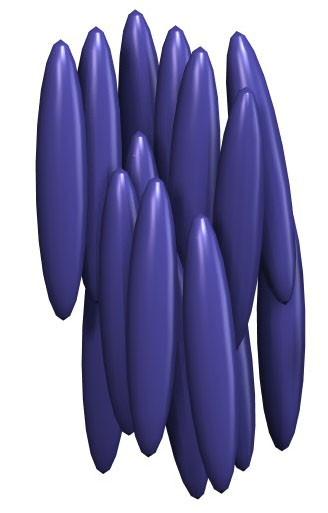
\includegraphics[height=7cm, width=\textwidth]{Nematic_example}
		{А}
	\end{minipage}
	\hfill
	\begin{minipage}{0.49\textwidth}
		\centering
		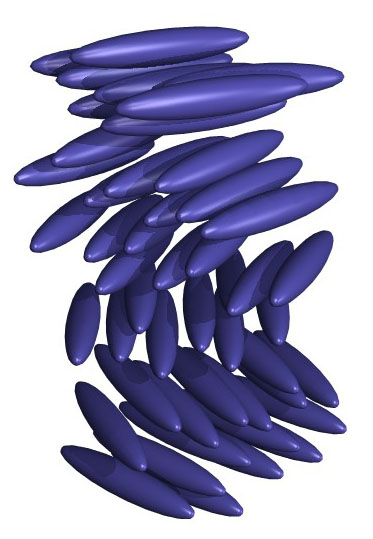
\includegraphics[height=7cm, width=\textwidth]{Cholesteric_example}
		{Б}
	\end{minipage}
	\vspace{0.5cm}
	\caption{Схематическое изображение НЖК (А) и ХЖК (Б)}
\end{figure}

Важной особенностью ЖК является способность к переориентации во внешнем поле, как в магнитном, так и в электрическом.
Это явление, открытое в 1927 году, называется эффектом Фредерикса~\autocite{Fred1927,Fred1933}.
%Примером устройства, в основе работы которого лежит эффект Фредерикса, может служить \todo{TND (twisted nematic device)}
Именно это свойство позволяет использовать ЖК для создания различных электрооптических устройств: систем вывода информации (дисплеев), переключаемых дифракционных решёток, очков и окон с изменяемой светопропускной способностью, беззеркальных лазеров и т.д.~\cite{Blinov1994, McManamon1996, Taheri2000, F.2001, Schmidtke2003, Senyuk2005, Jiang2019}.

Несмотря на то, что эффект Фредерикса изучался в течение долгого времени и для ряда случаев описан как теоретически, так и экспериментально для различных фаз: нематической, холестерической и т.д.~\cite{pikin, deGennesbook1995, stewartBook}, в последнее десятилетие интерес к его изучению возрос~\cite{Brown2003, Brown2007, Makarov2010, Garbovskiy2017, dosSantos2019, Begum2020}.
Большинство исследований идут в сторону усложнения систем и условий, в которых они находятся: рассматриваются различные типы ЖК, геометрии ячеек и граничные условия.
Это в первую очередь связано с возможностью создания систем, обладающих заданными свойствами для потенциальных технических приложений.
При этом наибольший интерес представляют напряжения, индуцирующие переход, а также трансформация равновесной структуры при напряжении выше порогового, так как именно от пространственного распределения директора зависят оптические свойства ячейки.
Важно отметить, что теоретические описания перехода Фредерикса значительно отличаются для магнитного и электрического полей, так как электрическое поле оказывается неоднородным внутри ячейки ЖК~\autocite{Deuling,NonHomoElectricField1972,CTBerr,Arakelyan1984,Napoli2006}.
Ранее переход Фредерикса в нематиках рассматривался как фазовый переход второго рода~\autocite{Guyon1975}, то есть непрерывный фазовый переход.
Однако оказалось, что в киральных нематиках (холестериках) этот переход может быть как непрерывным, так и разрывный, в зависимости от значений материальных констант~\autocite{VAR2013}.

Ещё одно важное свойство ЖК заключается в появлении дополнительной поляризации в результате искажения поля директора.
Такую поляризацию называют \textit{флексоэлектрической}.
%Поляризацию, появляющуюся в ЖК в результате искажения поля директора, называют \textit{флексоэлектрической}.
Первым теоретически описал это явление Майер в 1969 году~\cite{Meyer1969}.
Он дал объяснение~\textit{дипольному} механизму появления флексоэлектрической поляризации для молекул клино- или банановидной формы, обладающих собственным дипольным моментом (см. Рис.~\ref{pic-Meyer}). 

\begin{figure}[ht]
	\centering
	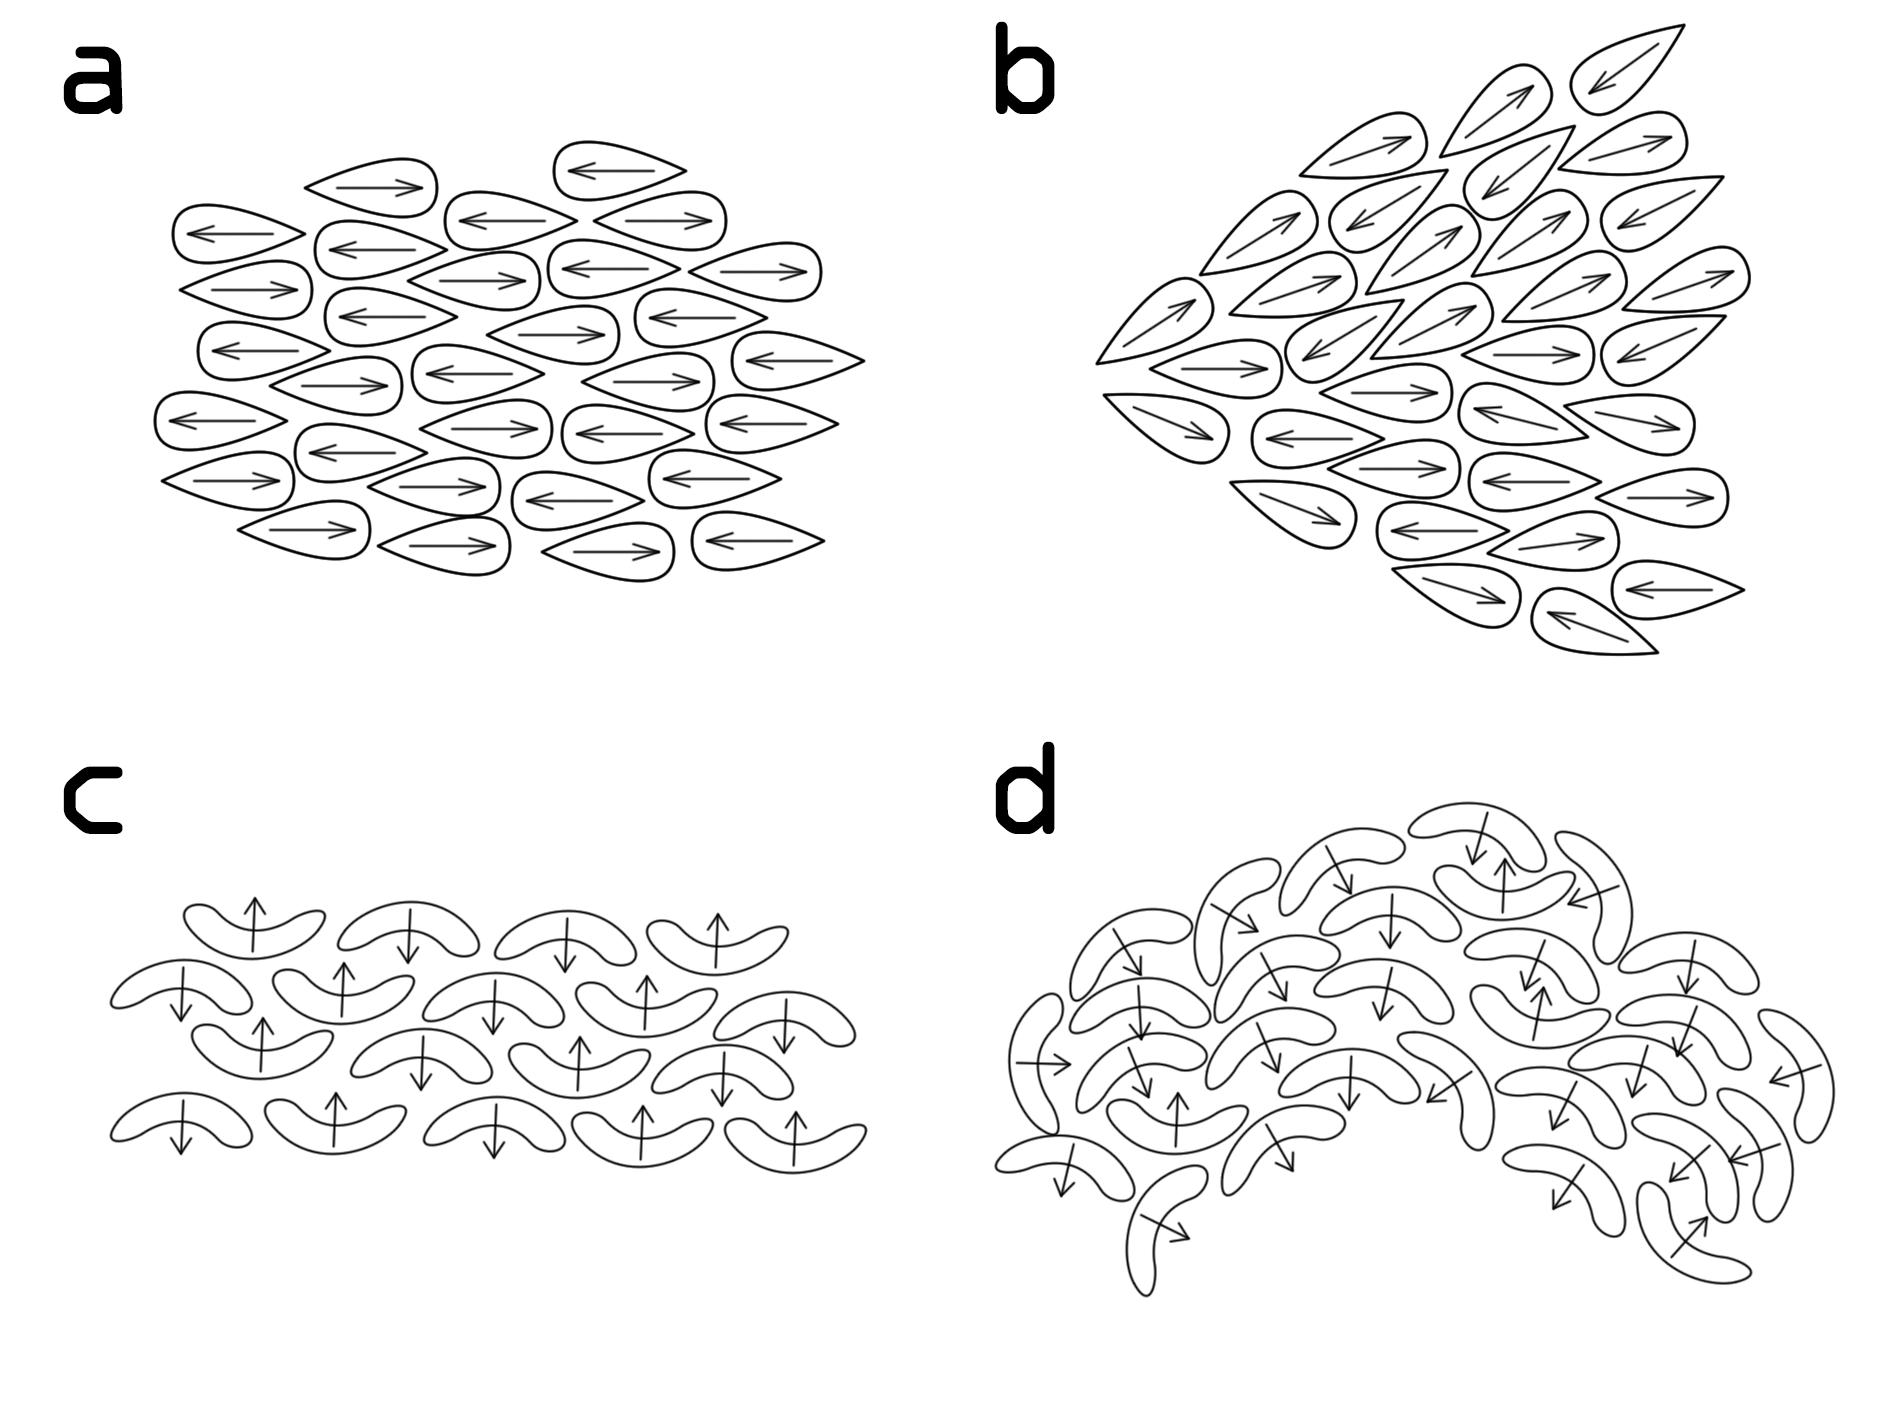
\includegraphics[width=14cm]{Molecules}
	\caption{Появление флексоэлектрической поляризации у молекул специальной формы. Неискажённые состояния для молекул соответственно клиновидной (a) и банановидной (c) формы. Поперечный изгиб, флексоэлектрическая поляризация направлена вправо (b). Продольный изгиб, флексоэлектрическая поляризация направлена вниз (d).}
	\label{pic-Meyer}
\end{figure}

Однако, как показал Прост в 1977 году, этот механизм не является единственным~\cite{Prost77}.
Он объяснил второй известный ныне механизм флексоэлектричества -- квадрупольный.
На рис.~\ref{Prost_explanation}a изображена неискажённая структура из молекул, не обладающих собственным дипольным моментом, но обладающих квадрупольным моментом, причём поляризация в каждом слое равна нулю.
На рис.~\ref{Prost_explanation}b изображена группа таких же молекул, которые подвержены деформации поперечного изгиба.
Видно, что в верхней части области 2 положительный заряд увеличен за счёт квадруполя из области 1.
В то же время, положительный заряд внизу области 2 уменьшился за счёт того, что квадруполи частично перешли в область 3.
Таким образом, данная структура начинает обладать собственным дипольным моментом, направленным вверх, и к ней можно применить всё то, что было сказано про полярные молекулы.
\begin{figure}[ht]
	\centering
	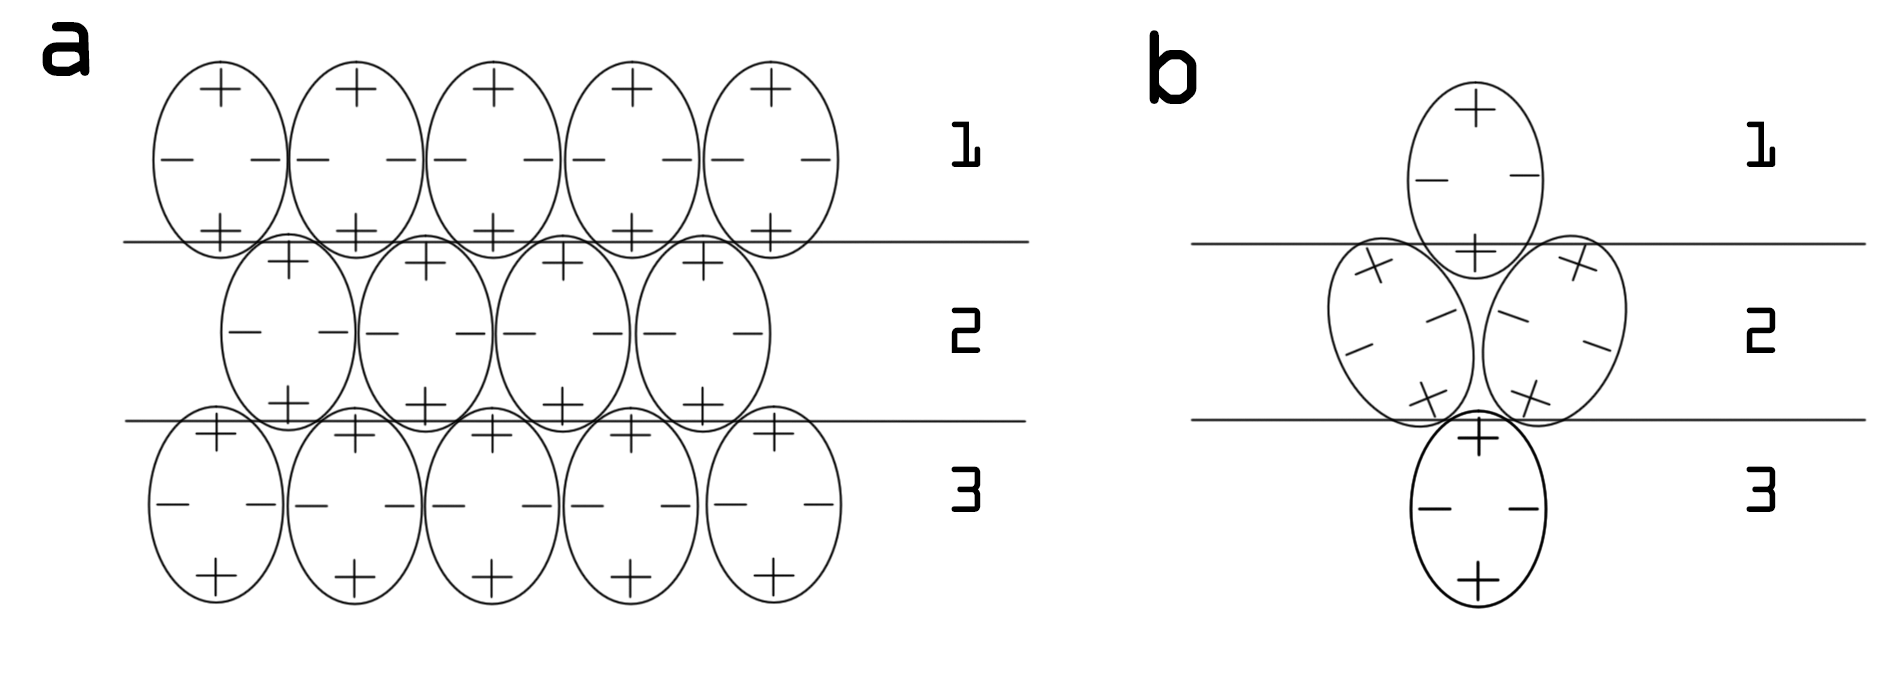
\includegraphics[width=17cm]{Prost_explanation}
	\caption{Симметричные молекулы -- поперечный изгиб}
	\label{Prost_explanation}
\end{figure}

Данная работа посвящена изучению влияния внешнего электрического поля на ориентационную структуру ХЖК с учётом флексоэлектрического эффекта.
Рассматривается ячейка, представляющая собой две проводящие плоскопараллельные пластины, к которым приложено некоторое напряжение; пространство между ними заполнено ХЖК, и ось спирали перпендикулярна ограничивающим плоскостям.
В данной работе исследуется влияние флексоэлектрической поляризации на напряжение, индуцирующее переход Фредерикса в ХЖК при различных параметрах системы, таких как сумма флексоэлектрических коэффициентов,симметричные и несимметричные мягкие граничные условия и др. В первом разделе рассмотрено выражение для свободной энергии ХЖК, отдельно рассмотрен вклад флексоэлектрической поляризации, получены уравнения Эйлера-Лагранжа на равновесную конфигурацию ХЖК, исключён из описания азимутальный угол.
Во втором разделе для случая отрицательной анизотропии диэлектрической проницаемости при помощи численной минимизации функционала свободной энергии найдены равновесные конфигурации при различных условиях.
Также аналитически рассмотрена устойчивость основного состояния ХЖК (планарной геликоидальной структуры).
В третьем разделе аналитически рассмотрен случай, когда вкладом упругой энергии Франка можно пренебречь по сравнению с вкладом, возникающим из-за флексоэлектричества и взаимодействия с электрическим полем, приводится схема возможных трансформаций ориентационной структуры ЖК в зависимости от соотношения материальных параметров системы.
\if 0
\todo{РАЗДЕЛИТЕЛЬ}
Эффект молекулярной переориентации в ячейках жидких кристаллов (ЖК), вызванной внешним полем, широко исследуется, во многом благодаря многообразию приложений.
Это явление, известное как переход (эффект) Фредерикса \textcolor{blue}{был открыт в конце 1920-х годов.(ссылки)}
Среди устройств, в основе работы которых лежит эффект Фредерикса, можно выделить, например, ЖК-дисплеи, переключаемые дифракционные решётки, беззеркальные лазеры и другие~\autocite{YangWu2014}. 
Переход Фредерикса изучался для различных полей: статического электрического и магнитного полей, осциллирующего электрического поля, лазерного излучения, а также для ЖК в различных фазах: нематической, холестерической, смектической и т.~д.~\autocite{Blinov1994,deGennesbook1995,stewartBook}

Простейшим способом учёта взаимодействия с границами является случай жёстких граничных условий.
Слабое зацепление обычно описывается потенциалом Рапини-Папулара~\autocite{Rapini69}.
Важно отметить, что теоретические описания перехода Фредерикса значительно отличаются для магнитного и электрического полей, так как электрическое поле оказывается неоднородным внутри ячейки ЖК~\autocite{Deuling,NonHomoElectricField1972,CTBerr,Arakelyan1984,Napoli2006}.
Ранее переход Фредерикса в нематиках рассматривался как фазовый переход второго рода~\autocite{Guyon1975}, то есть непрерывный фазовый переход.
Однако оказалось, что в киральных нематиках (холестериках) этот переход может быть как непрерывным, так и \todo{разрывный}, в зависимости от материальных констант~\autocite{VAR2013}.

В последнее время наблюдается растёт интерес к изучению влияния флексоэлектричества~\autocite{buka2012flexoelectricity} на пороговые эффекты в ЖК, например, на переключение бистабильных ЖК-устройств~\autocite{Davidson2002,  Parry-Jones2009, Cummings2013}.
Благодарю флексоэлектричеству возникает дополнительное искажение электрического поля, таким образом, оно тоже влияет на переход Фредерикса.
Такой переход в нематических ЖК (НЖК) изучался в работах~\autocite{Brown2003,Brown2007,Mema2017}.
Анализ при этом ограничивался жёсткими граничными условиями, а также приближением низшей гармоники для объёмного распределения директора и электрического поля.

\todo{ДАЛЬШЕ -- ЧТО СДЕЛАНО В РАБОТЕ PRE2018}
Данная работа посвящена теоретическому изучению перехода Фредерикса в случае статического электрического поля в плоскопараллельной ячейке холекстерического ЖК (ХЖК) с учётом флексоэлектрического эффекта, конечной энергии зацепления, а также неоднородности электрического поля внутри ячейки.
При этом задача состоит в нахождении следующих параметров: пороговые напряжения, равновесная конфигурация директора при напряжении выше напряжения перехода \todo{[просто равновесной конфигурации директора?]}, а также род перехода.
Отдельный акцент сделан на устойчивости равновесных структур, а также на построении фазовых диаграмм.

Работа построена следующим образом. В \todo{Секции $N$} выводится выражение для свободной энергии плоскопараллельной ячейки ЖК\todo{, подключённой к источнику}\todo{[, в виде суммы поверхностных и объёмных вкладов]}.
При этом учитывается неоднородность электрического поля внутри ячейки, вызванная диэлектрической анизотропией ЖК и флексоэлектричеством.
Поверхностная свободная энергия описывается потенциалом Рапини-Папулара.
В \todo{Секции $N+1$} находится равновесное распределение директора для широкого спектра материальных констант.
Также при помощи численного вариационного анализа построены фазовые диаграммы, включая зоны стабильности и метастабильности.
В \todo{Секции $N+2$} аналитически изучается устойчивость планарной геликоидальной структуры.
В \todo{Секции $N+3$} исследуется род перехода Фредерикса с использованием двухпараметрической модели Ландау.
В \todo{Секции $N+4$} содержится подведение итогов и обсуждение результатов.
% Счётчик \texttt{citeexternal} используется для подсчёта процитированных публикаций.
\fi
 % Характеристика работы по структуре во введении и в автореферате не отличается (ГОСТ Р 7.0.11, пункты 5.3.1 и 9.2.1), потому её загружаем из одного и того же внешнего файла, предварительно задав форму выделения некоторым параметрам

%\textbf{Объем и структура работы.} Диссертация состоит из~введения, трёх глав,
%заключения и~двух приложений.
%% на случай ошибок оставляю исходный кусок на месте, закомментированным
%Полный объём диссертации составляет  \ref*{TotPages}~страницу
%с~\totalfigures{}~рисунками и~\totaltables{}~таблицами. Список литературы
%содержит \total{citenum}~наименований.
%
%Полный объём диссертации составляет
%\formbytotal{TotPages}{страниц}{у}{ы}{}, включая
%\formbytotal{totalcount@figure}{рисун}{ок}{ка}{ков} и
%\formbytotal{totalcount@table}{таблиц}{у}{ы}{}.   Список литературы содержит
%\formbytotal{citenum}{наименован}{ие}{ия}{ий}.
    % Введение
\ifnumequal{\value{contnumfig}}{1}{\counterwithout{figure}{chapter}
}{\counterwithin{figure}{chapter}}
\ifnumequal{\value{contnumtab}}{1}{\counterwithout{table}{chapter}
}{\counterwithin{table}{chapter}}
\chapter{Свободная энергия искажения ориентационной структуры}\label{ch:ch1}

В данной работе изучается изменение ориентационной структуры ХЖК, находящегося между двумя плоскопараллельными пластинами, расположенными на расстоянии  $L$ друг от друга. Ограничивающие пластины считаются проводящими, и к ним подведено постоянное напряжение $U$, таким образом, система имеет вид плоского конденсатора. При изменении напряжения $U$ может меняться ориентация директора в ячейке. Изучению таких трансформаций структуры будет уделено основное внимание.
\begin{figure}[ht]
	\centering
	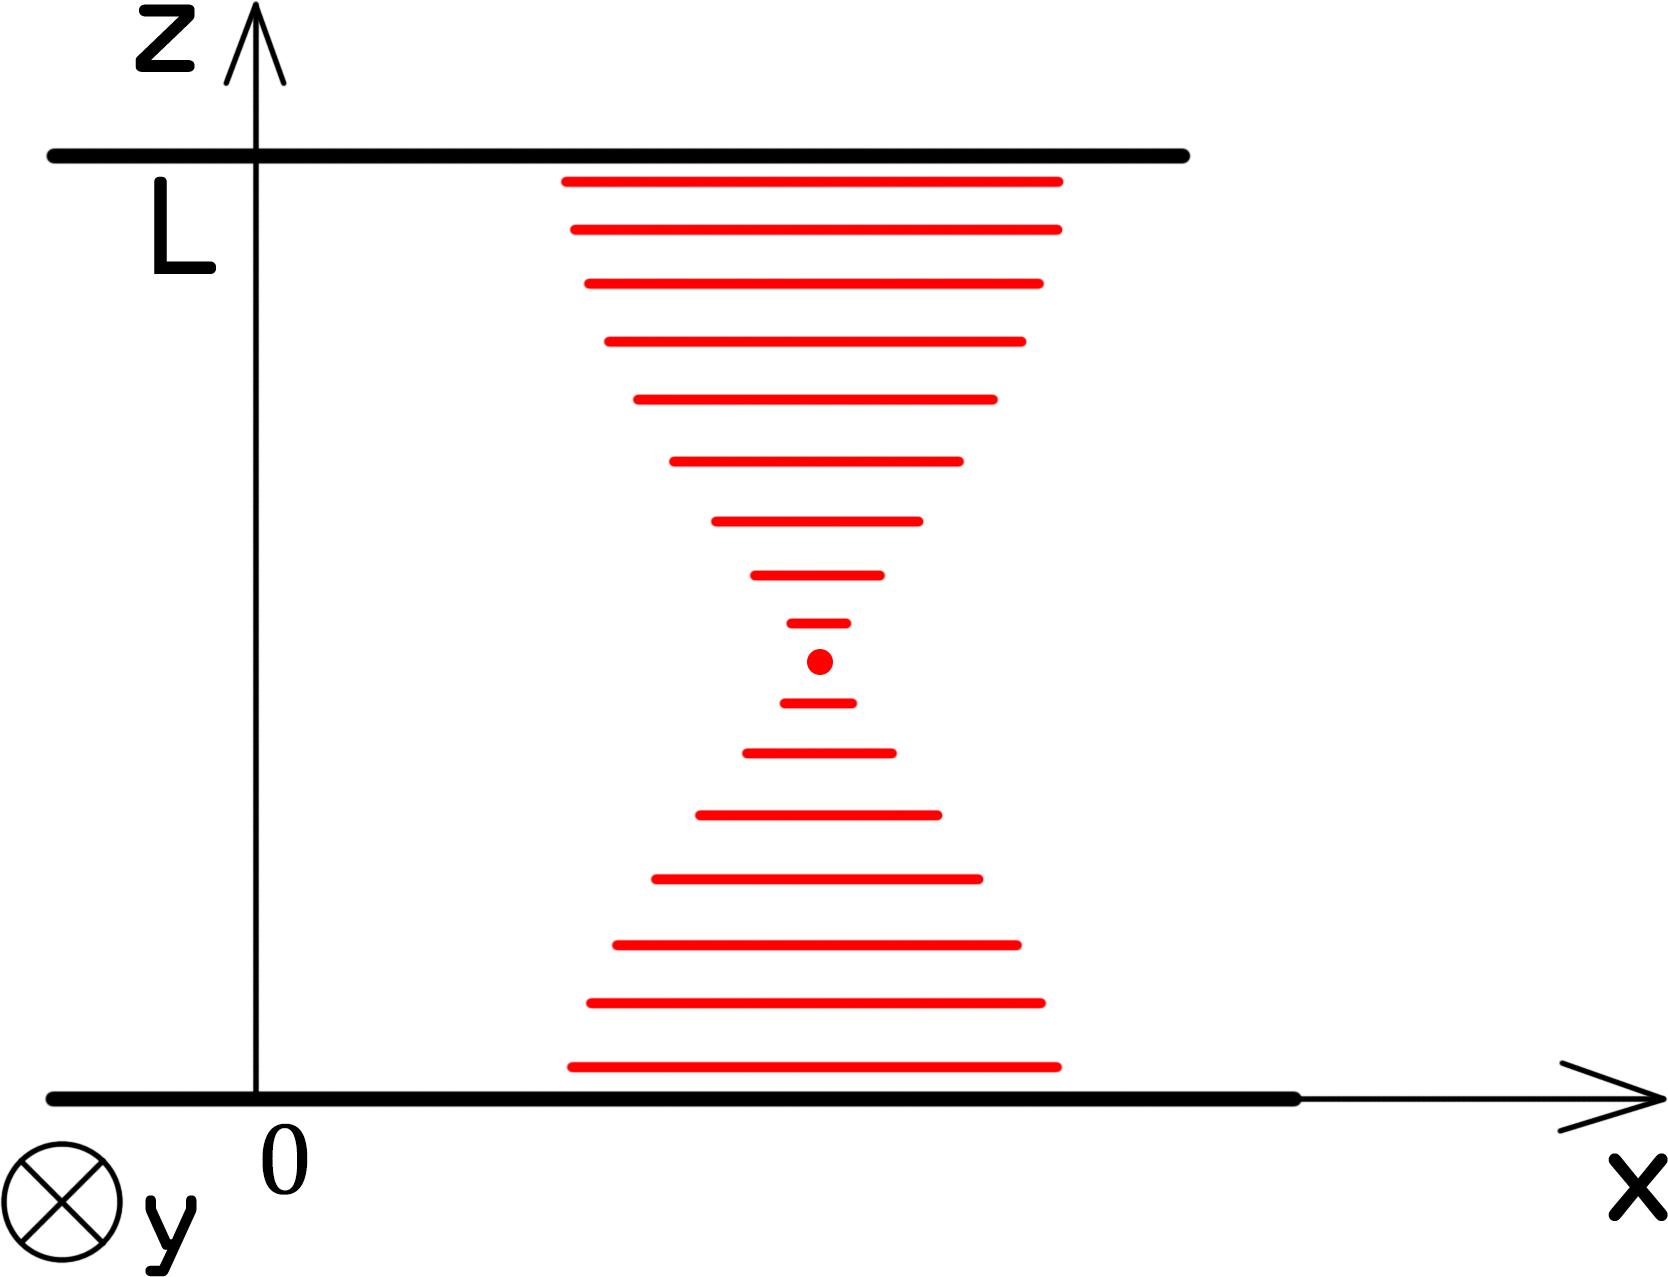
\includegraphics[width=10cm]{decart}
	\caption{Декартова система координат для ячейки ХЖК с планарной геликоидальной структурой.}
	\label{pic:decart}
\end{figure}

Введём декартову систему координат с осью $z$, направленной перпендикулярно пластинам (Рис.~\ref{pic:decart}).
Предположим, что размер ограничивающих пластин значительно превосходит расстояния $L$ между ними, таким образом, можно пренебречь краевыми эффектами.
Также предположим, что все физические характеристики рассматриваемой системы однородны в плоскости $XY$ и зависят только от координаты $z$: $\textbf{n}(\textbf{r}) = \textbf{n} (z)$, $\textbf{E} = \textbf{E}(z)$, где $\bb{E}$ - напряжённость электрического поля.

Свободная энергия ХЖК, связанная с искажением ориентационной структуры директора, может быть представлена в виде суммы четырёх слагаемых~\eqref{F_tot very basic}
\begin{equation}
\FF_\mathrm{tot} = \FF_\mathrm{e} + \FF_\mathrm{sf} + \FF_\mathrm{f} + \FF_\mathrm{flex}.
\label{F_tot very basic}
\end{equation}
Здесь $\FF_\mathrm{e}$ -- вклад в свободную энергию, связанный с ориентационной упругостью в объёме, $\FF_\mathrm{sf}$ -- упругая энергия сцепления молекул ЖК с ограничивающими поверхностями, $\FF_\mathrm{f}$ -- энергия ЖК как диэлектрика во внешнем электрическом поле, $\FF_\mathrm{flex}$ -- вклад в свободную энергию, обусловленный взаимодействием флексоэлектрической поляризации с внешним электрическим полем. Эти слагаемые можно естественным образом разделить на две группы: обусловленные ориентационной упругостью (первые два слагаемых в~\eqref{F_tot very basic}) и возникающие из-за взаимодействия ЖК с внешним полем (третье и четвёртое слагаемые в~\eqref{F_tot very basic}).

\section{Свободная энергия упругих искажений ориентационной структуры}\label{sec:ch1/sec1}
Первое слагаемое в~\eqref{F_tot very basic}, свободная энергия упругих ориентационных искажений $\FF_e$, было впервые описано в работах Озена~\autocite{Oseen1933} и Цохера~\cite{Zocher1933} и более подробно изучено Франком~\autocite{Frank1958}. Этот вклад может быть записан как~\cite{deGennesbook1995}
\begin{equation}
\FF_\mathrm{e} = \frac{S_\perp}{2} \int\limits_{l_1}^{l_2}\left[ K_{11} (\diver{\textbf{n}})^2 + K_{22} (\textbf{n}\rot{\textbf{n}} + q_0)^2 + K_{33} (\textbf{n}\times \rot{\textbf{n}})^2 \right]\, dz.
\label{F_e from n}
\end{equation}
Здесь $S_{\perp}$ -- площадь ограничивающих пластин, $K_{ii}$ -- модули Франка, $\pi/q_0$ -- период геликоидальной спирали ХЖК.
Физический смысл констант $K_{ii}$ удобно пояснить на примере свободной энергии Франка для нематического ЖК, которая получается из~\eqref{F_e from n} при $q_0 = 0$.
Тогда каждое из трёх слагаемых подынтегрального выражения соответствует искажениям определённого типа.
При деформации поперечного изгиба (Рисунок~\ref{distortions}a) в правой части~\eqref{F_e from n} остаётся только слагаемое с $K_{11}$.
При деформации кручения (Рисунок~\ref{distortions}b) в правой части~\eqref{F_e from n} остаётся только слагаемое с $K_{22}$.
Наконец, при деформации продольного изгиба (Рисунок~\ref{distortions}c) остаётся только слагаемое с $K_{33}$.
Таким образом, $K_{11}$, $K_{22}$ и $K_{33}$ являются модулями поперечного изгиба, кручения и продольного изгиба соответственно.

\begin{figure}
	\centering
	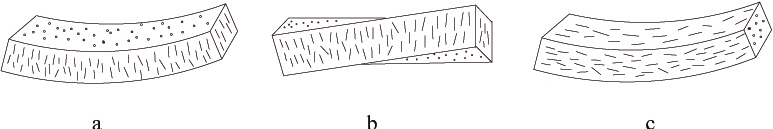
\includegraphics[width=15cm]{ThreeDistortions}
	\caption{Различные типы деформаций поля директора в ЖК: a -- поперечный изгиб, b -- кручение, c -- продольный изгиб.}
	\label{distortions}
\end{figure}

Для дальнейшего анализа свободной энергии удобно представить декартовы координаты директора $\bb{n}(z)$ как функции полярного угла $\theta(z)$ и азимутального угла $\varphi(z)$ (Рисунок~\ref{Coords}):
\begin{equation}
\bb{n} = 
\begin{pmatrix}
\sin{\theta}\cos{\phi}\\
\sin{\theta}\sin{\phi}\\
\cos{\theta}
\end{pmatrix}.
\end{equation}

\begin{figure}[ht]
	\centering
	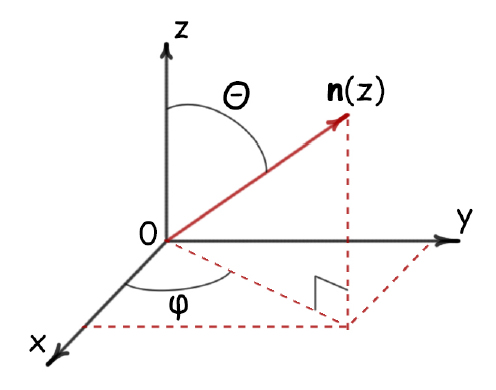
\includegraphics[width=7cm]{pic_04}
	\caption{Полярный $\theta(z)$ и азимутальный $\phi(z)$ углы директора $\bb{n}(z)$.}
	\label{Coords}
\end{figure}
Для $\diver{\bb{n}}$ и $\rot{\bb{n}}$ имеем:
\begin{equation}
\begin{split}
&\diver{\bb{n}} = -\theta' \sin{\theta},\\
&\rot{\bb{n}} = \begin{pmatrix}-\theta'\cos{\theta}\sin{\phi}-\phi'\sin{\theta}\cos{\phi}\\\theta'\cos{\theta}\cos{\phi}-\phi'\sin{\theta}\sin{\phi}\\0\end{pmatrix}.
\end{split}
\label{div and rot}
\end{equation}
Здесь штрихом обозначена производная по $z$. Подставляя~\eqref{div and rot} в~\eqref{F_e from n}, получаем
\begin{equation}
\FF_\mathrm{e} =\FF^\mathrm{(0)}_{e} + \frac{S_\perp}{2} \int\limits_{0}^{L}\left[ \AA(\theta) (\theta')^2 + \BB(\theta) (\phi ' )^2 - \CC(\theta)\phi' \right]\, dz.
\label{eq:F_e_basic}
\end{equation}
\begin{equation}
\begin{aligned}[c]
\AA (\theta) &= K_{11}\sin^2{\theta} + K_{33}\cos^2{\theta},\\
\BB (\theta) &= \sin^2{\theta} \left( K_{22}\sin^2{\theta} + K_{33}\cos^2{\theta}  \right),\\
\CC (\theta) &= q_0 K_{22}\sin^2{\theta}.
\end{aligned}
\end{equation}
где $\FF^\mathrm{(0)}_{e} = VK_{22}q_0^2/2$, а $V = S_\bot L$ -- это объём ячейки.

Второе слагаемое в выражении~\eqref{F_tot very basic} -- энергия сцепления ХЖК с подложкой:
\begin{equation}
\FF_\mathrm{sf} = \frac{S_\perp}{2}\sum\limits_{\alpha=1,2} w_\alpha \left( \textbf{n}(l_\alpha),\, \textbf{n}^{(\alpha)}_0 \right), \quad l_1 = 0, \quad l_2 = L.
\label{F_bound very basic}
\end{equation}
Здесь индекс $\alpha = 1,2$ нумерует границы, скалярные функции $w_\alpha$  зависят от направлений директора на границах ячейки $\textbf{n}(l_\alpha)$, а также от направления осей лёгкого ориентирования $\textbf{n}^{(\alpha)}_0$.
Важное свойство функций $w_\alpha$ в~\eqref{F_bound very basic} -- обращение соответствующей функции в ноль, если $\bb{n}(l_\alpha) = \bb{n}^{(\alpha)}_0$. Конкретный вид $w_\alpha$ выбирается в соответствии с решаемой задачей.
Так, в случае малых отклонений $\bb{n}(l_\alpha)$ от $\bb{n}^{(\alpha)}_0$ возможно использование квадратичной аппроксимации по разности этих векторов:
\begin{equation}
w_\alpha(\bb{n}(l_\alpha),\ \bb{n}^{(\alpha)}_0) = w_\alpha(\bb{n}(l_\alpha) - \bb{n}^{(\alpha)}_0) = (\bb{n}(l_\alpha) - \bb{n}^{(\alpha)}_0) \hat{W}_\alpha (\bb{n}(l_\alpha) - \bb{n}^{(\alpha)}_0)
\label{Square_approximation_matrices}
\end{equation}
Здесь $\hat{W}_\alpha$ -- положительно определённые матрицы размера $3\times 3$.
Потенциал~\eqref{Square_approximation_matrices} является квадратичным по отклонениям директора на границах. Также применяется потенциал, квадратичный по отклонениям углов и использованный, например, в~\cite{VAR2013}:
\begin{equation}
w_\alpha(\theta_\alpha,\phi_\alpha, \theta_0^{(\alpha)}, \phi_0^{(\alpha)}) = W^{(\alpha)}_\theta \left( \theta_\alpha - \theta^{(\alpha)}_0 \right)^2 + W^{(\alpha)}_\phi \left( \phi_\alpha - \phi^{(\alpha)}_0 \right)^2.
\label{Square_approximation}
\end{equation}
Здесь $W^{(\alpha)}_{\theta,\, \phi} > 0$ -- константы сцепления с подложкой, $\theta^{(\alpha)}_0$ и $\phi^{(\alpha)}_0$ -- углы лёгкого ориентирования на границах, также введены обозначения: $\theta_1 = \theta(0)$, $\phi_1 = \phi(0)$, $\theta_2 = \theta(L)$, $\phi_2 = \phi(L)$.
Часто используется потенциал, который был предложен Рапини и Папуларом в 1969 году~\cite{Rapini69}:
\begin{equation}
w_\alpha(\theta_\alpha,\phi_\alpha, \theta_0^{(\alpha)}, \phi_0^{(\alpha)}) = W^{(\alpha)}_\theta \sin^2 \left( \theta_\alpha - \theta^{(\alpha)}_0 \right) + W^{(\alpha)}_\phi \sin^2 \left( \phi_\alpha - \phi^{(\alpha)}_0 \right)
\label{RP_anchoring}
\end{equation}
Заметим, что в низшем (квадратичном) приближении потенциалы~\eqref{Square_approximation} и~\eqref{RP_anchoring} совпадают.
Для описания сцепления с подложкой в задачах, связанных с деформацией шага спирали ХЖК, удобен B-потенциал, предложенный в работах~\cite{Belyakov2004, Belyakov2006}:
\begin{equation}
w_\alpha(\phi_\alpha, \phi_0^{(\alpha)}) = - W_\phi^{(\alpha)}\left( \cos^2\frac{\phi_\alpha - \phi_0^{(\alpha)}}{2} - \frac{1}{2} \right)
\label{B-potential}
\end{equation}
Также отметим, что если энергия сцепления с подложкой много больше остальных вкладов, то константы $W_{\theta}^{(\alpha)}$ и $W_{\phi}^{(\alpha)}$ устремляются к бесконечности, и положение директора на границах фиксируется.
В таком случае говорят о жёстких граничных условиях.

В данной работе используется потенциал Рапини-Папулара~\eqref{RP_anchoring}:
\begin{equation}
\FF_\mathrm{sf} = \frac{S_\perp}{2}\sum\limits_{\alpha=1,2} W^{(\alpha)}_\theta \sin^2 \left( \theta_\alpha - \theta^{(\alpha)}_0 \right) + W^{(\alpha)}_\phi \sin^2 \left( \phi_\alpha - \phi^{(\alpha)}_0 \right)
\label{eq:F_sf final}
\end{equation}

\section{Энергия взаимодействия с полем}\label{sec:ch1/sec2}
Третье слагаемое в выражении~\eqref{F_tot very basic} -- энергия электрического поля в диэлектрике:
\begin{equation}
\FF_\mathrm{f} = -\frac{S_\perp}{2} \int\limits_0^L \frac{(\hat{\varepsilon}\bb{E},\, \textbf{E})}{4\pi}\, dz.
\label{F_f very basic}
\end{equation}
Тензор диэлектрической проницаемости в одноосном ЖК имеет следующий вид~\eqref{eps in LC}:
\begin{equation*}
\epsilon_{ij} = \epsilon_\parallel n_i n_j + \epsilon_\perp (\delta_{ij} - n_i n_j),
\label{eps in LC}
\end{equation*}
где $\epsilon_\parallel$ и $\epsilon_\perp$ -- диэлектрические проницаемости вдоль и поперёк директора. Здесь индексы $i$ и $j$ принимают значения $1$, $2$, $3$, что соответствует пространственным координатам $x$, $y$, $z$.

Наконец, последний вклад в~\eqref{F_tot very basic} возникает благодаря флексоэлектрической поляризации.
Наиболее общее выражение $i$-ой компоненты вектора флексоэлектрической поляризации $\bb{P}^\mathrm{flex}$ можно, с учётом малости искажений ориентационной структуры, записать следующим образом:
\begin{equation}
P^\mathrm{flex}_i = f_{ijk} \partial_k n_j,
\label{P_fl_basic}
\end{equation}
здесь подразумевается суммирование по повторящимся значкам.
Тензор $f_{ijk}$, называемый флексоэлектрическим, должен состоять из компонент дирекора $\bb{n}$ и символов Кронекера.
Так как $\bb{n}$ и $-\bb{n}$ эквивалентны, свободная энергия должна быть инвариантна относительно этой замены. Значит, тензор $f_{ijk}$ может содержать в себе только нечётные степени компонент директора.
Таким образом, наиболее общее выражение для $f_{ijk}$:
\begin{equation}
f_{ijk} = e_1 n_i \delta_{jk} + e_2 n_j \delta_{ik} + e_3 n_k \delta_{ij} + e_4 n_i n_j n_k,
\label{f_ijk basic}
\end{equation}
где $e_1$, $e_2$, $e_3$, $e_4$ -- флексоэлектрические коэффициенты.
Подставляя~\eqref{f_ijk basic} в~\eqref{P_fl_basic}, получаем следующие четыре слагаемых:
\begin{align*}
&e_1 n_i \delta_{jk} \partial_k n_j = e_1 n_i \partial_j n_j = e_1 n_i \diver{\textbf{n}},\\
&e_2 n_j \delta_{ik} \partial_k n_j = e_2 n_j\partial_i n_j = 0,\\
&e_3 n_k \delta_{ij} \partial_k n_j = e_3 (\textbf{n},\, \nabla)n_i = e_3\left[\rot{\textbf{n}}\times \textbf{n}\right]_i,\\
&e_4 n_i n_j n_k \partial_k n_j = 0.
\end{align*}
Здесь учтено, что $n_i \partial_j n_i = 0$, так как $\textbf{n}^2 = 1$.
Вектор флексоэлектрической поляризации записывается в виде
\begin{equation}
\textbf{P}^\mathrm{flex} = e_1 \textbf{n}\diver{\textbf{n}} + e_3 \left[ \rot{\textbf{n}} \times \textbf{n} \right].
\label{P_fl through n}
\end{equation}

Таким образом, вклад флексоэлектрической поляризации в свободную энергию можно записать как
\begin{equation}
\FF_\mathrm{flex} = - S_\bot \int\limits_0^L (\bb{P}^\mathrm{flex},\, \bb{E})\, dz.
\end{equation}

Вводя в вектор электрической индукции помимо диэлектрической поляризации $\bb{P}$ ещё и флексоэлектрическую $\bb{P}^\mathrm{flex}$, имеем
\begin{equation}
\bb{D} = \bb{E} + 4\pi\bb{P} + 4\pi \bb{P}^\mathrm{flex} = \hat{\varepsilon}\bb{E} + 4\pi \bb{P}^\mathrm{flex} 
\end{equation}
Для вектора электрической индукции в одноосной среде можно написать:	
\begin{equation}
\textbf{D} = \epsilon_\perp \textbf{E}+\epsilon_a (\textbf{E},\, \textbf{n})\textbf{n} + 4\pi \textbf{P}^\mathrm{flex},\quad \epsilon_{a} = \epsilon_\parallel - \epsilon_\perp,
\label{D and E from n}
\end{equation}
где $\epsilon_a$ -- величина анизотропии диэлектрической проницаемости, а $\textbf{P}^\mathrm{flex}$ -- флексоэлектрическая поляризация~\cite{deGennesbook1995}, возникающая благодаря искажениям поля директора ХЖК. 

Таким образом, выражение для энергии взаимодействия ХЖК с внешним электрическим полем имеет вид:
\begin{equation*}
\FF_\mathrm{E} = \FF_\mathrm{f} + \FF_\mathrm{flex}= - \frac{S_\bot}{8\pi} \int\limits_0^L (\bb{E},\, \hat{\varepsilon}\bb{E})\, dz - S_\bot \int\limits_0^L (\bb{P}^\mathrm{flex},\, \bb{E})\, dz
\end{equation*}
Как следует из уравнения Максвелла $\rot {\bf E} = 0$ и граничных условий ${E}_{x,y}(0)={E}_{x,y}(L)= 0$, единственная ненулевая компонента вектора ${\bf E}$ -- это $E_z=E(z)$.
Таким образом, $\bb{P}^\mathrm{flex} \bb{E} = P^\mathrm{flex}_z E_z$. Учитывая, что $P^\mathrm{flex}_z = (e_1 + e_3)n_z \partial_z n_z$ и подставляя~\eqref{Coords}, можно записать для вклада в свободную энергию
\begin{equation}\label{eqF_f_pref}
\FF_\mathrm{E} = -\frac{S_{\!\bot}}{8\pi}\int_{0}^{L}E^2(z){\EE}(\theta)dz
+ S_{\!\bot}\bar{e}\int_{0}^{L}
\sin 2\theta \,\theta' E(z) dz,
\end{equation}
где введены обозначения
\begin{equation}\label{111}
\EE(\theta) = \ve_\bot + \ve_a \cos^2\theta,\; \bar{e}=(e_1+e_3)/2.
\end{equation}
Из другого уравнения Максвелла, $\diver {\bf D}(z) = 0$, следует, что $z$-компонента вектора электрической индукции $D_z$ не зависит от $z$.
Совмещая это с выражениями~\eqref{Coords} и~\eqref{D and E from n}, получаем
\begin{equation}\label{E_z=D_z}
D_z=\EE(\theta)E(z) - 4\pi\bar{e}\sin 2\theta \,\theta',
\end{equation}
откуда можно выразить
\begin{equation}\label{eqE_z}
E(z)=\left(D_z + 4\pi\bar{e}\sin2\theta \, \theta'\right)/{\EE}(\theta).
\end{equation}
Напряжение на обкладках $U$ и $z$-компонента вектора электрической индукции $D_z$ связаны следующим образом:
\begin{equation}
U = \int_0^L E(z)\, dz
=D_z J^{-1}+ 4\pi\bar{e} J_1,
\end{equation}
где введены следующие обозначения:
\begin{equation}\label{D_z=UJ}
J^{-1}= \int_0^L \frac{dz}{\EE(\theta)},\quad J_1=\varepsilon_a^{-1}\ln\frac{{\EE}(\theta(0))}{{\EE}(\theta(L))}.
\end{equation}
Отметим, что $J_1$ зависит только от значений $\theta(z)$ на границах, $\theta(0)$ и $\theta(L)$. Таким образом, для $D_z$ имеем:
\begin{equation}\label{eqD_z}
D_z =\left(U-4\pi\bar{e} J_1\right)J,
\end{equation}
а выражение для электрического поля имеет вид
\begin{equation}\label{eqE(z)inhomo=final}
E(z)=\left(UJ+ 4\pi\bar{e}(\sin2\theta \, \theta'-J_1J) \right)/{\EE}(\theta).
\end{equation}
Из выражения~\eqref{eqE(z)inhomo=final} следует, что в ориентационно неоднородной среде с флексоэлектрическими свойствами может возникать ненулевое электрическое поле даже если $U = 0$.
Подставляя Eq.~\eqref{eqE(z)inhomo=final} в Eq.~\eqref{eqF_f_pref}, получаем итоговое выражение для энергии электрического поля в ячейке ХЖК:
\begin{equation}\label{eq_F_f_final1}
\FF_\mathrm{E}=-\frac{S_{\!\bot}}{8\pi}U^2 J +S_{\!\bot} \bar{e}U JJ_1 +2\pi S_{\!\bot} \bar{e}^2\left(\int_{0}^{L}\frac{(\sin 2\theta \,\theta')^2}{{\EE}(\theta)}dz -JJ_1^2\right).
\end{equation}
Важно отметить, что в формуле~\eqref{eq_F_f_final1} учтена неоднородность электрического поля, возникающая из-за наличия флексоэлектричества.
Кроме того, видно, что помимо первых двух слагаемых, зависящих от напряжения $U$, в~\eqref{eq_F_f_final1} присутствуют ещё два слагаемых, зависящих только от ориентационной структуры.
Для случая $\bar{e}=0$ выражение для энергии записывается так же, как, например, в работах~\cite{Deuling,NonHomoElectricField1972,VAR2013}:
\begin{equation}\label{E_field}
\FF_\mathrm{E} = - S_{\!\bot} U^2 J/{8\pi}.
\end{equation}
В случае, когда $(\varepsilon_a/\varepsilon_\bot)\cos^2\theta\ll 1$ формула~\eqref{E_field} сводится к более простому виду~\cite{deGennesbook1995}
\begin{equation}
\FF_\mathrm{E} =\FF_\mathrm{E}^{(0)} -\frac{S_{\!\bot} \varepsilon_a U^2}{8\pi L^2} \int_0^L \cos^2\theta\, dz,\;\FF_\mathrm{E}^{(0)} =-\frac{S_{\!\bot} U^2\varepsilon_\bot}{8\pi L},
\end{equation}
при этом учитывается неоднородность поля директора ${\bf n}(z)$, а электрическое поле в ячейке считается однородным.

Заметим, что энергия $\FF_\mathrm{E}$ зависит от знака напряжения $U$ из-за одного из флексоэлектрических членов, $S_{\!\bot} \bar{e}U JJ_1$.
В случае жёстких симметричных граничных уловий, $\theta(0) = \theta(L)$, этот вклад исчезает благодаря тому, что $J_1 = 0$.
Отметим, что случай $\bar{e} < 0$ сводится к $\bar{e} > 0$ при помощи замены $(\bar{e}, U)\rightarrow (-\bar{e}, -U)$.
Таким образом, можно ограничиться рассмотрением только случая $\bar{e} > 0$.

Подставляя~\eqref{eq:F_e_basic},~\eqref{eq:F_sf final} и~\eqref{eq_F_f_final1} в~\eqref{F_tot very basic}, получаем выражение для свободной энергии ячейки ХЖК во внешнем электрическом поле
\begin{multline}
\FF_\mathrm{tot} ={\FF^{(0)}_e}+ \frac{S_{\!\bot}}{2} \int_{0}^{L}\Big[ \AA(\theta) (\theta')^2 + B(\theta) (\phi ' )^2
- 2C(\theta)\phi' \Big]\, dz +\\
\,+ \frac{S_{\!\bot}}{2}\sum\limits_{\alpha=1,2} \left[W_\theta^{(\alpha)} {\sin^2\big( \theta - \theta_0^{(\alpha)}\big)}\right.
+ \left.W_\phi^{(\alpha)}{\sin^2 \big( \phi - \phi_0^{(\alpha)} \big)}\right] -\\
-S_{\!\bot} \EuScript{U}^2J/8\pi, \label{eq:free-energy}
\end{multline}
где
\begin{equation}\label{eqAAtilde}
\AA(\theta) =A(\theta) +4\pi \bar{e}^2{\sin^22\theta}/{\EE}(\theta),\; \EuScript{U}=U-4\pi \bar{e}J_1,
\end{equation}


\section{Система уравнений Эйлера-Лагранжа и упрощение функционала свободной энергии}\label{sec:ch2/sec1}
Первая вариация свободной энергии~\eqref{eq:free-energy} может быть записана следующим образом:
\begin{multline}
	\delta \FF_\mathrm{tot} = S_{\!\bot} \left\{\int_0^L \left[ {\frac12\frac{d\AA}{d\theta}\, \theta'^2 \delta\theta + \AA\theta' \delta\theta'} + \frac12\frac{d B}{d\theta}\,\phi'^2\delta\theta\right. + \right.\\
	\left.+ B \phi' \delta \phi'- \frac{d C}{d\theta}\,\phi'\delta\theta - C\delta\phi'\right]\, dz + \\
	{+\frac12\!\sum_{\alpha=1,2}\left(W_\theta^{(\alpha)}\!\sin2(\theta_\alpha- \theta_0^{(\alpha)})\delta\theta_\alpha + W_\phi^{(\alpha)}\!\sin2(\phi_\alpha - \phi_0^{(\alpha)})\delta\phi_\alpha\right)} + \\
	\left. {+\frac{\varepsilon_a}{8\pi} \EuScript{U}^2J^2\int_0^L \frac{\sin 2\theta }{\EE^{2}(\theta)}\delta\theta\, dz
		+\left.\bar{e}\EuScript{U} J \frac{\sin 2\theta }{\EE(\theta)}\delta\theta\right|^L_0
	}\right\}.
	\label{deltaF_tot}
\end{multline}
Проинтегрировав по частям вклады в $\delta\FF_\mathrm{tot}$, содержащие вариации производных и приравнивая к нулю $\delta \FF_\mathrm{tot}$ для произвольных вариаций $\delta\theta$ и $\delta\phi$ в объёме и на границах, получаем систему из двух уравнений Эйлера-Лагранжа 
\begin{eqnarray}
	&&\frac{d\AA}{d\theta}\theta'^2 + 2\AA \theta'' = \frac{d B}{d\theta}\phi'^2 - 2\frac{d C}{d\theta}\phi'
	+ \frac{\varepsilon_a\EuScript{U}^2\! J ^2\!\sin 2\theta}{4\pi\EE^2(\theta)} ,
	\label{eq:E-L1}\\
	&&{d}\left( B\phi' - C \right)/{dz} = 0,
	\label{eq:E-L2}
\end{eqnarray}
и двух граничных условий
\begin{eqnarray}
	&&\left(2(-1)^\alpha [{\AA(\theta)\theta'} + \bar{e} {\EuScript{U}}J\sin2\theta/\EE(\theta)]\phantom{ W_\phi^{(\alpha)}}\right. + \nonumber\\
	&&\hspace{27mm}\left.\left.+ W_\theta^{(\alpha)}\sin2(\theta - \theta_0^{(\alpha)})\right) \right|_{z=l_\alpha} = 0,\label{eq:gran-1}\\
	&&{\left.\left(2(-1)^\alpha (B\phi' - C)
		+W_\phi^{(\alpha)}\sin2(\phi - \phi_0^{(\alpha)})\right) \right|_{z=l_\alpha}} = 0,
	\label{eq:gran-2}
\end{eqnarray}
где $\alpha = 1, 2$.
Из уравнений~\eqref{eq:E-L1} и~\eqref{eq:E-L2} можно сделать вывод, что функция $\theta(z)\in C^2[0,\, L]$, а $\phi(z)\in C^1[0,\, L]$.
Заметим, что~\eqref{eq:E-L1} -- функциональное интегро-дифференциальное уравнение, так как $J_1$ зависит от значений $\theta(z)$ на границах, а $J$ содержит интеграл~\eqref{eqD_z}.
Кроме того, граничные условия~\eqref{eq:gran-1} являются нелокальными.
Данные свойства, как уравнения, так и граничных условий, возникли благодаря учёту флексоэлектрической поляризации.

Первый интеграл системы уравнений~\eqref{eq:E-L1} и~\eqref{eq:E-L2} выглядит следующим образом:
\begin{eqnarray}
	&&{\AA(\theta)\theta'^2}+  B(\theta)\varphi'^2 {-\EuScript{U}^2 J ^2/(4\pi\EE(\theta))} =C_1,
	\label{eq:theta'}\\
	&&B(\theta)\phi' -C(\theta)= C_2,
	\label{eq:phi'}
\end{eqnarray}
где $C_{1,2}$ -- произвольные константы.
Конкретные значения этих констант могут быть найдены из граничных условий~\eqref{eq:gran-1} и~\eqref{eq:gran-2}.

Ввиду сложности возникающих уравнений Эйлера-Лагранжа удобно искать равновесную ориентационную структуру ХЖК, используя прямые методы минимизации свободной энергии.
При этом уравнение~\eqref{eq:phi'} и граничные условия~\eqref{eq:gran-2} позволяют упростить выражение для полной свободной энергии $\FF_\mathrm{tot}$, а уравнение~\eqref{eq:theta'} и граничные условия~\eqref{eq:gran-1} дают возможность контролировать точность результатов численных расчётов.
В решении задачи поиска равновесных профилей углов оказывается возможным записать $\FF_\mathrm{tot}$ как функционал, зависящий только от $\theta(z)$.
Для этого используем выражение для $\phi'$, полученное из соответствующего уравнения Эйлера-Лагранжа.
Таким образом, мы будем рассматривать $\FF_\mathrm{tot}[\theta(z)]$, содержащий равновесное распределение $\phi(z)$, подстраивающееся под заданное распределение $\theta(z)$.
%Ограничиваясь только равновесными профилями углов $\theta(z)$ и $\phi(z)$, можно записать $\FF_\mathrm{tot}$ как функционал, зависящий только от $\theta(z)$.

Рассмотрим выражение~\eqref{eq:F_e_basic} для свободной энергии, связанной с объёмной ориентационной упругостью ХЖК.
Подставив в него $\phi'$, выраженное из~\eqref{eq:phi'}, получим
\begin{equation}
	\FF_\mathrm{e} = \FF^{(0)}_\mathrm{e} + \frac{S_{\!\bot}}{2}\int_0^L \left[ A(\theta) \theta'^2 + \frac{C_2^2 - C^2(\theta)}{B(\theta)} \right]\, dz.
	\label{eq:F_e_2}
\end{equation}
В выражение~\eqref{eq:F_e_2} входит константа $C_2$.
Для того, чтобы определить её, проинтегрируем $\phi'$ из~\eqref{eq:phi'} по отрезку $[0,L]$:
\begin{equation}
	\phi_\mathrm{tot} = C_2 I_1 + I_2,
	\label{eq:help_find_C1-2}
\end{equation}
где $\phi_\mathrm{tot}  =  \phi(L) - \phi(0)$,
$$
I_1 = \int_0^L \frac{dz}{B(\theta)}, \;
I_2  =  \int_0^L \frac{C(\theta)}{B(\theta)}\, dz.
$$
Подставляя~\eqref{eq:phi'} в~\eqref{eq:gran-2}, получаем
\begin{equation}
	{2\left(\phi(l_\alpha)-\phi_0^{(\alpha)}\right)=(-1)^{\alpha+1}\arcsin\left(2C_2/W_\phi^{(\alpha)}\right)},
	\label{eq:help_find_C1-0}
\end{equation}
$\alpha=1,2$, следовательно,
\begin{equation}
	\!\!{2(\phi_\mathrm{tot}^{(0)}-\phi_\mathrm{tot})
		=\arcsin({2C_2}/{W_{\phi}^{(1)}})+\arcsin({2C_2}/{W_{\phi}^{(2)}})},
	\label{eq:help_find_C1}
\end{equation}
где $\phi_\mathrm{tot}^{(0)}=\phi_0^{(2)}-\phi_0^{(1)}$.
Здесь предполагается, что $\left|\phi(l_\alpha)-\phi_0^{(\alpha)}\right|\leq \pi/4$.
Это ограничение соответствует отсутствию скачкообразных изменений шага спирали ХЖК~\autocite{BelyakovJumpsPhysRevE2005}.

Из~\eqref{eq:help_find_C1-2} и \eqref{eq:help_find_C1} можно выразить константу $C_2$,
\begin{equation}\label{eq:C2iteration}
	C_2=(\varphi_\textrm{tot}^{(0)}-I_2)/\big(I_1+k_1/W^{(1)}_\varphi + k_2/W^{(2)}_\varphi \big),
\end{equation}
где $k_\alpha=\left(W^{(\alpha)}_\varphi/2C_2\right)\arcsin\left(2C_2/W^{(\alpha)}_\varphi \right)$, $1\leq k_\alpha\leq \pi/2$.
Неравенства $\left|C_2\right|/W^{(\alpha)}_\varphi \leq 0.5$ должны выполняться, чтобы существовало решение трансцендентного уравнения~\eqref{eq:C2iteration}.
Для случая $\left|C_2\right|/W^{(\alpha)}_\varphi \ll 1$ можно записать точное выражение для $C_2$:
\begin{equation}\label{eq:C2implicit}
	{C_2=(\varphi_\textrm{tot}^{(0)}-I_2)\left(I_1+{2}/{W_\phi^{H}}\right)^{-1}}
\end{equation}
где $W_\phi^{H} = {2W_\phi^{(1)}W_\phi^{(2)}}/(W_\phi^{(1)} + W_\phi^{(2)})$.


Подставляя выражение~\eqref{eq:C2iteration} в~\eqref{eq:F_e_2} и используя~\eqref{eq:help_find_C1-0}, получаем следующее выражение для полной свободной энергии $\FF_\mathrm{tot}$ как функционала, зависящего только от $\theta(z)$:
\begin{multline}
	\FF_\mathrm{tot}(\theta) = \FF^{(0)}_e + \frac{S_{\!\bot}}{2}\Bigg[\int_0^L \left({ \AA(\theta)}\theta'^2 - \frac{C^2(\theta)}{B(\theta)} \right) dz +\\
	+W_\theta^{(1)}\sin^2 \left( \theta(0) - \theta_0^{(1)} \right)+W_\theta^{(2)}\sin^2 \left( \theta(L) - \theta_0^{(2)} \right) +\\
	+
	C_2^2\left(I_1+{\kappa_1}/{W^{(1)}_\varphi}+{\kappa_2}/{W^{(2)}_\varphi}\right)-{\frac{\EuScript{U}^2 J}{4\pi} }\Bigg],
	\label{eq:F_for_minimization}
\end{multline}
где $\kappa_\alpha=2/\Big(1+\sqrt{1-\big(2C_2/W^{(\alpha)}_\varphi\big)^2}\Big)$, $1\leq \kappa_\alpha\leq 2$.
При $\left|C_2\right|/W^{(\alpha)}_\varphi \ll 1$ предпоследнее слагаемое в~\eqref{eq:F_for_minimization} может быть приближённо записано как
\begin{equation}\label{LastTermFtot_theta_implicit}
	\frac{S_{\!\bot}}{2}\left( \phi_\mathrm{tot}^{(0)} - I_2 \right)^2\left(I_1+{2}/{W_\phi^{H}}\right)^{-1}.
\end{equation}
Погрешность такой аппроксимации составляет около 2\% при $\left|C_2\right|/W^{(\alpha)}_\varphi \leq 0.25$ и около 15\% для всей области $\left|C_2\right|/W^{(\alpha)}_\varphi\leq 1/2$.

После нахождения равновесной функции $\theta(z)$ можно найти соответствующую равновесную функцию $\phi(z)$, совмещая выражения~\eqref{eq:phi'}, \eqref{eq:gran-2} и~\eqref{eq:C2iteration}:
\begin{equation}\label{eq:phi_profile}
	\varphi(z)=\varphi_0^{(1)}+\frac12\arcsin\frac{2C_2}{W^{(1)}_\varphi}
	+ \int_0^z \frac{C(\theta)+C_2}{B(\theta)}\, dz .
\end{equation}           % Глава 1
%\chapter{Переход Фредерикса и изменение равновесной ориентационной структуры ХЖК во внешнем электрическом поле.}\label{ch:ch2}
\section{Система уравнений Эйлера-Лагранжа и упрощение функционала свободной энергии}\label{sec:ch2/sec1}
Первая вариация свободной энергии~\eqref{eq:free-energy} может быть записана следующим образом:
\begin{multline}
\delta \FF_\mathrm{tot} = S_{\!\bot} \left\{\int_0^L \left[ {\frac12\frac{d\AA}{d\theta}\, \theta'^2 \delta\theta + \AA\theta' \delta\theta'} + \frac12\frac{d B}{d\theta}\,\phi'^2\delta\theta\right. + \right.\\
\left.+ B \phi' \delta \phi'- \frac{d C}{d\theta}\,\phi'\delta\theta - C\delta\phi'\right]\, dz + \\
{+\frac12\!\sum_{\alpha=1,2}\left(W_\theta^{(\alpha)}\!\sin2(\theta_\alpha- \theta_0^{(\alpha)})\delta\theta_\alpha + W_\phi^{(\alpha)}\!\sin2(\phi_\alpha - \phi_0^{(\alpha)})\delta\phi_\alpha\right)} + \\
\left. {+\frac{\varepsilon_a}{8\pi} \EuScript{U}^2J^2\int_0^L \frac{\sin 2\theta }{\EE^{2}(\theta)}\delta\theta\, dz
	+\left.\bar{e}\EuScript{U} J \frac{\sin 2\theta }{\EE(\theta)}\delta\theta\right|^L_0
}\right\}.
\label{deltaF_tot}
\end{multline}
Проинтегрировав по частям вклады в $\delta\FF_\mathrm{tot}$, содержащие вариации производных и приравнивая к нулю $\delta \FF_\mathrm{tot}$ для произвольных вариаций $\delta\theta$ и $\delta\phi$ в объёме и на границах, получаем систему из двух уравнений Эйлера-Лагранжа 
\begin{eqnarray}
&&\frac{d\AA}{d\theta}\theta'^2 + 2\AA \theta'' = \frac{d B}{d\theta}\phi'^2 - 2\frac{d C}{d\theta}\phi'
+ \frac{\varepsilon_a\EuScript{U}^2\! J ^2\!\sin 2\theta}{4\pi\EE^2(\theta)} ,
\label{eq:E-L1}\\
&&{d}\left( B\phi' - C \right)/{dz} = 0,
\label{eq:E-L2}
\end{eqnarray}
и двух граничных условий
\begin{eqnarray}
&&\left(2(-1)^\alpha [{\AA(\theta)\theta'} + \bar{e} {\EuScript{U}}J\sin2\theta/\EE(\theta)]\phantom{ W_\phi^{(\alpha)}}\right. + \nonumber\\
&&\hspace{27mm}\left.\left.+ W_\theta^{(\alpha)}\sin2(\theta - \theta_0^{(\alpha)})\right) \right|_{z=l_\alpha} = 0,\label{eq:gran-1}\\
&&{\left.\left(2(-1)^\alpha (B\phi' - C)
	+W_\phi^{(\alpha)}\sin2(\phi - \phi_0^{(\alpha)})\right) \right|_{z=l_\alpha}} = 0,
\label{eq:gran-2}
\end{eqnarray}
где $\alpha = 1, 2$.
Из уравнений~\eqref{eq:E-L1} и~\eqref{eq:E-L2} можно сделать вывод, что функция $\theta(z)\in C^2[0,\, L]$, а $\phi(z)\in C^1[0,\, L]$.
Заметим, что~\eqref{eq:E-L1} -- функциональное интегро-дифференциальное уравнение, так как $J_1$ зависит от значений $\theta(z)$ на границах, а $J$ содержит интеграл~\eqref{eqD_z}.
Кроме того, граничные условия~\eqref{eq:gran-1} являются нелокальными.
Данные свойства, как уравнения, так и граничных условий, возникли благодаря учёту флексоэлектрической поляризации.

Первый интеграл системы уравнений~\eqref{eq:E-L1} и~\eqref{eq:E-L2} выглядит следующим образом:
\begin{eqnarray}
&&{\AA(\theta)\theta'^2}+  B(\theta)\varphi'^2 {-\EuScript{U}^2 J ^2/(4\pi\EE(\theta))} =C_1,
\label{eq:theta'}\\
&&B(\theta)\phi' -C(\theta)= C_2,
\label{eq:phi'}
\end{eqnarray}
где $C_{1,2}$ -- произвольные константы.
Конкретные значения этих констант могут быть найдены из граничных условий~\eqref{eq:gran-1} и~\eqref{eq:gran-2}.

Ввиду сложности возникающих уравнений Эйлера-Лагранжа удобно искать равновесную ориентационную структуру ХЖК, используя прямые методы минимизации свободной энергии.
При этом уравнение~\eqref{eq:phi'} и граничные условия~\eqref{eq:gran-2} позволяют упростить выражение для полной свободной энергии $\FF_\mathrm{tot}$, а уравнение~\eqref{eq:theta'} и граничные условия~\eqref{eq:gran-1} дают возможность контролировать точность результатов численных расчётов.
В решении задачи поиска равновесных профилей углов оказывается возможным записать $\FF_\mathrm{tot}$ как функционал, зависящий только от $\theta(z)$.
Для этого используем выражение для $\phi'$, полученное из соответствующего уравнения Эйлера-Лагранжа.
Таким образом, мы будем рассматривать $\FF_\mathrm{tot}[\theta(z)]$, содержащий равновесное распределение $\phi(z)$, подстраивающееся под заданное распределение $\theta(z)$.
%Ограничиваясь только равновесными профилями углов $\theta(z)$ и $\phi(z)$, можно записать $\FF_\mathrm{tot}$ как функционал, зависящий только от $\theta(z)$.

Рассмотрим выражение~\eqref{eq:F_e_basic} для свободной энергии, связанной с объёмной ориентационной упругостью ХЖК.
Подставив в него $\phi'$, выраженное из~\eqref{eq:phi'}, получим
\begin{equation}
\FF_\mathrm{e} = \FF^{(0)}_\mathrm{e} + \frac{S_{\!\bot}}{2}\int_0^L \left[ A(\theta) \theta'^2 + \frac{C_2^2 - C^2(\theta)}{B(\theta)} \right]\, dz.
\label{eq:F_e_2}
\end{equation}
В выражение~\eqref{eq:F_e_2} входит константа $C_2$.
Для того, чтобы определить её, проинтегрируем $\phi'$ из~\eqref{eq:phi'} по отрезку $[0,L]$:
\begin{equation}
\phi_\mathrm{tot} = C_2 I_1 + I_2,
\label{eq:help_find_C1-2}
\end{equation}
где $\phi_\mathrm{tot}  =  \phi(L) - \phi(0)$,
$$
I_1 = \int_0^L \frac{dz}{B(\theta)}, \;
I_2  =  \int_0^L \frac{C(\theta)}{B(\theta)}\, dz.
$$
Подставляя~\eqref{eq:phi'} в~\eqref{eq:gran-2}, получаем
\begin{equation}
{2\left(\phi(l_\alpha)-\phi_0^{(\alpha)}\right)=(-1)^{\alpha+1}\arcsin\left(2C_2/W_\phi^{(\alpha)}\right)},
\label{eq:help_find_C1-0}
\end{equation}
$\alpha=1,2$, следовательно,
\begin{equation}
\!\!{2(\phi_\mathrm{tot}^{(0)}-\phi_\mathrm{tot})
	=\arcsin({2C_2}/{W_{\phi}^{(1)}})+\arcsin({2C_2}/{W_{\phi}^{(2)}})},
\label{eq:help_find_C1}
\end{equation}
где $\phi_\mathrm{tot}^{(0)}=\phi_0^{(2)}-\phi_0^{(1)}$.
Здесь предполагается, что $\left|\phi(l_\alpha)-\phi_0^{(\alpha)}\right|\leq \pi/4$.
Это ограничение соответствует отсутствию скачкообразных изменений шага спирали ХЖК~\autocite{BelyakovJumpsPhysRevE2005}.

Из~\eqref{eq:help_find_C1-2} и \eqref{eq:help_find_C1} можно выразить константу $C_2$,
\begin{equation}\label{eq:C2iteration}
C_2=(\varphi_\textrm{tot}^{(0)}-I_2)/\big(I_1+k_1/W^{(1)}_\varphi + k_2/W^{(2)}_\varphi \big),
\end{equation}
где $k_\alpha=\left(W^{(\alpha)}_\varphi/2C_2\right)\arcsin\left(2C_2/W^{(\alpha)}_\varphi \right)$, $1\leq k_\alpha\leq \pi/2$.
Неравенства $\left|C_2\right|/W^{(\alpha)}_\varphi \leq 0.5$ должны выполняться, чтобы существовало решение трансцендентного уравнения~\eqref{eq:C2iteration}.
Для случая $\left|C_2\right|/W^{(\alpha)}_\varphi \ll 1$ можно записать точное выражение для $C_2$:
\begin{equation}\label{eq:C2implicit}
{C_2=(\varphi_\textrm{tot}^{(0)}-I_2)\left(I_1+{2}/{W_\phi^{H}}\right)^{-1}}
\end{equation}
где $W_\phi^{H} = {2W_\phi^{(1)}W_\phi^{(2)}}/(W_\phi^{(1)} + W_\phi^{(2)})$.


Подставляя выражение~\eqref{eq:C2iteration} в~\eqref{eq:F_e_2} и используя~\eqref{eq:help_find_C1-0}, получаем следующее выражение для полной свободной энергии $\FF_\mathrm{tot}$ как функционала, зависящего только от $\theta(z)$:
\begin{multline}
\FF_\mathrm{tot}(\theta) = \FF^{(0)}_e + \frac{S_{\!\bot}}{2}\Bigg[\int_0^L \left({ \AA(\theta)}\theta'^2 - \frac{C^2(\theta)}{B(\theta)} \right) dz +\\
+W_\theta^{(1)}\sin^2 \left( \theta(0) - \theta_0^{(1)} \right)+W_\theta^{(2)}\sin^2 \left( \theta(L) - \theta_0^{(2)} \right) +\\
+
C_2^2\left(I_1+{\kappa_1}/{W^{(1)}_\varphi}+{\kappa_2}/{W^{(2)}_\varphi}\right)-{\frac{\EuScript{U}^2 J}{4\pi} }\Bigg],
\label{eq:F_for_minimization}
\end{multline}
где $\kappa_\alpha=2/\Big(1+\sqrt{1-\big(2C_2/W^{(\alpha)}_\varphi\big)^2}\Big)$, $1\leq \kappa_\alpha\leq 2$.
При $\left|C_2\right|/W^{(\alpha)}_\varphi \ll 1$ предпоследнее слагаемое в~\eqref{eq:F_for_minimization} может быть приближённо записано как
\begin{equation}\label{LastTermFtot_theta_implicit}
\frac{S_{\!\bot}}{2}\left( \phi_\mathrm{tot}^{(0)} - I_2 \right)^2\left(I_1+{2}/{W_\phi^{H}}\right)^{-1}.
\end{equation}
Погрешность такой аппроксимации составляет около 2\% при $\left|C_2\right|/W^{(\alpha)}_\varphi \leq 0.25$ и около 15\% для всей области $\left|C_2\right|/W^{(\alpha)}_\varphi\leq 1/2$.

После нахождения равновесной функции $\theta(z)$ можно найти соответствующую равновесную функцию $\phi(z)$, совмещая выражения~\eqref{eq:phi'}, \eqref{eq:gran-2} и~\eqref{eq:C2iteration}:
\begin{equation}\label{eq:phi_profile}
\varphi(z)=\varphi_0^{(1)}+\frac12\arcsin\frac{2C_2}{W^{(1)}_\varphi}
+ \int_0^z \frac{C(\theta)+C_2}{B(\theta)}\, dz .
\end{equation}

\section{Численная минимизация функционала свободной энергии}
Равновесную ориентационную структуру в ячейке ХЖК будем искать с помощью численной минимизации свободной энергии~\eqref{eq:F_for_minimization}, используя следующие углы лёгкого ориентирования на границах:
\begin{equation}\label{eq:initial}
\theta_0^{(1)}=\theta_0^{(2)}={\pi}/{2},\;\phi_\mathrm{tot}^{(0)}=q_0L.
\end{equation}
Эти условия соответствуют ненапряжённому ХЖК в отсутствие внешнего электрического поля.
Сведём задачу поиска минимума функционала $\FF_\mathrm{tot}[\theta(z)]$ к задаче поиска минимума функции нескольких переменных, аппроксимировав искомую зависимость $\theta(z)$ пробной функцией
\begin{equation}\label{eq:psi+Fourier}
\theta(z) =
\pi/2 + {\delta\psi}(z,\delta_1,\delta_2) + \sum\limits_{n=1}^N c_n\sin(\pi nz/L).
\end{equation}
Здесь слагаемое $\pi/2$ соответствует неискажённому состоянию.
Функция $\delta\psi(z,\delta_1,\delta_2)$, задаваемая выражением~\eqref{psi=}, содержит $\delta_1$ и $\delta_2$ -- отклонения от углов лёгкого ориентирования на границах: $\theta(0) = \pi/2 + \delta_1$, $\theta(L) = \pi/2 + \delta_2$.
Наконец, ряд Фурье описывает объёмные искажения ориентационной структуры, не затрагивающие границы.
Используя граничные условия~\eqref{eq:gran-1}, можно выразить коэффициенты $c_N$ и $c_{N-1}$ через все остальные -- $\delta_{1,2}$ и $\{c_n\}_{n=1}^{N-2}$.
Таким образом, углы $\delta_1$, $\delta_2$, а также коэффициенты $c_n$, $n=1,\dots,N-2$ являются регулируемыми параметрами.

Ограничимся в~\eqref{eq:psi+Fourier} $N = 20$ членами ряда Фурье.
Учёт более, чем 20 слагаемых приводит к относительному изменению профиля $\theta$ менее чем на $0.5\%$ для любого $z$ на всём интервале $[0,\, L]$.
В многомерной численной минимизации существует проблема попадания в максимумы или в седловые точки.
Для того, чтобы определить, действительно ли минимизация свободной энергии привела к минимуму, используем случайные небольшие сдвиги параметров  $\delta_{1,2}$, $\{c_n\}$ относительно полученных значений.
Если минимизационный алгоритм приводит к другому ответу, это означает, что предыдущий результат был ошибочным -- максимумом или седловой точкой.
При этом в случае, если достигнут, по крайней мере, локальный минимум, то при любом достаточно небольшом сдвиге минимизация будет всегда возвращать нас обратно.

Будем изменять напряжение $U$, зафиксировав все остальные параметры ячейки ЖК.
\begin{figure}
	\centering
	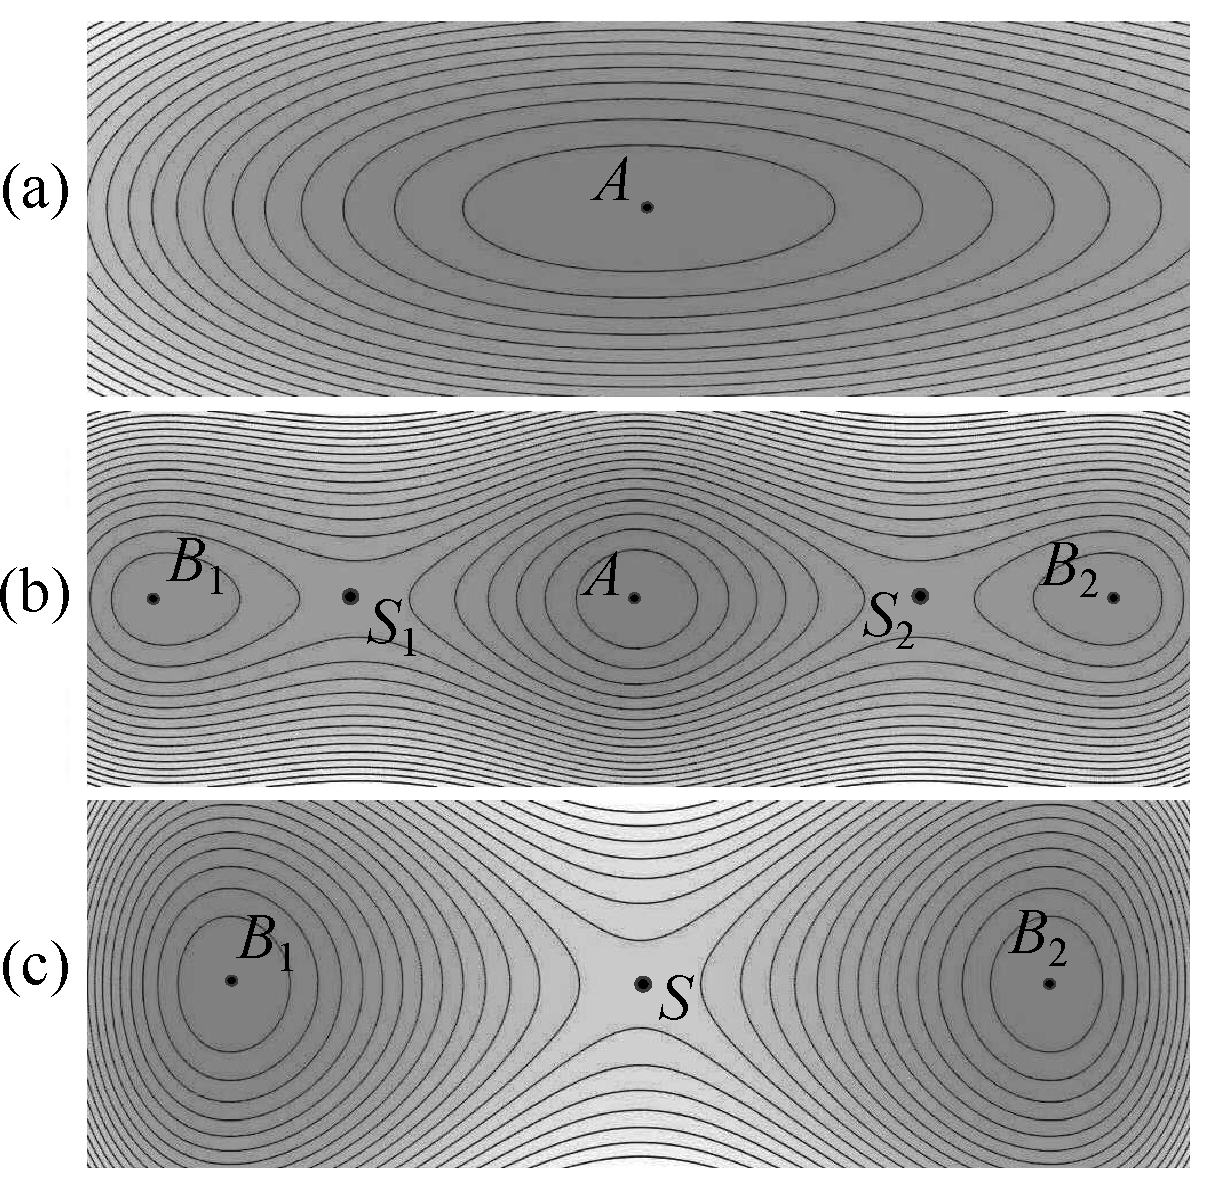
\includegraphics[width = 15cm]{Geo_final.eps}
	\caption{Схематичное двумерное изображение случаев, возникающих при численной минимизации свободной энергии}
	\label{pic_Geo_final}
\end{figure}
При этом будет наблюдаться один из трёх случаев, проиллюстрированных на Рис.~\ref{pic_Geo_final}:
\begin{enumerate}
	\item[(a)]
	Существует единственный минимум (точка А на рис.~\ref{pic_Geo_final}a), соответствующий планарной геликоидальной структуре, при этом $\delta_{1,2}=0$, $c_n = 0$, то есть $\theta(z)=\pi/2$, а $\phi(z) = q_0z$.
	\item[(b)]
	Случай трёх минимумов.
	Один из них (точка А на Рис.~\ref{pic_Geo_final}b) по-прежнему соответствует планарной геликоидальной структуре.
	Два других (точки $B_1$ и $B_2$) соответствуют искажённым структурам, то есть таким, для которых некоторые из параметров $\delta_{1,2}$, $c_n$ ненулевые.
	При этом параметры $(\delta_{1},\delta_{2},c_n)$, соответствующие точкам $B_1$ и $B_2$, отличаюся только знаком, следовательно, этим двум точкам соответствуют одинаковые распределения директора ввиду симметрии относительно замены ${\bf n} \leftrightarrow -{\bf n}$.
	\item[(c)]
	Имеются ровно два минимума.
	В этом случае существуют два минимума $B_1$ и $B_2$, соответствующие одной и той же искажённой ориентационной структуре.
	Планарная геликоидальная структура здесь не существует, так как является седловой точкой ($S$ на Рис.~\ref{pic_Geo_final}c).
\end{enumerate}
Здесь и далее мы будем называть ''устойчивыми'' равновесные состояния, соответствующие локальным минимумам свободной энергии, а ''метастабильными'' -- устойчивые состояния с энергией, большей, чем у другого устойчивого состояния.

\subsubsection{"Фазовая" \todo{(Структурная?)} диаграмма}

Случай (a) на Рис.~\ref{pic_Geo_final} возникает для напряжений $|U|$ ниже порогового значения $U^{**}$, а при достижении этого значения могут наблюдаться две различные ситуации.
Они соответствуют разрывному (I) и непрерывному (II) переходу Фредерикса:
\begin{itemize}
	\item[I.]
	В этом случае существует ещё одно пороговое значение $U^{*} > U^{**}$, при этом для $|U|\in (U^{**},\, U^{*})$ у функционала свободной энергииесть сразу три локальных минимума, из которых один соответствует начальной планарной геликоидальной структуре	, а два других -- искажённой ориентационной структуре, как показано на Рис.\ref{pic_Geo_final}b.
	Здесь $U^{**}$ -- наименьшее напряжение, при котором искажённая ориентационная структура ещё может существовать в качестве метастабильной, а, в свою очередь, $U^{*}$ -- максимальное напряжение, при котором планарная геликоидальная структура ещё может существовать как метастабильная.
	Таким образом, при любом $U$ из интервала $(U^{**},\,U^*)$ только одна из структур будет стабильной (с меньшей энергией), в то время как другая будет метастабильной.
	С ростом напряжения $|U|$ свободная энергия искажённой структуры уменьшается, и при $|U| = U_c$ становится равной энергии неискажённого состояния, и происходит разрывный переход Фредерикса.
	То есть, при $|U| < U_c$ более энергетически выгодным является неискажённое состояние, а при $|U| > U_c$ -- искажённое.
	Наконец, при $|U|>U^*$ реализуется случай (c).
	\item[II.]
	В данном сценарии существует только одно пороговое напряжение, $|U| = U_c$. Этот сценарий соответствует (I) для $U^{*} = U_c = U^{**}$, при этом происходит непрерывный переход Фредерикса. 
	Здесь при $|U| < U_c$ возникает случай (a), а при  $|U|>U_c$ -- случай (c), показанные на Рис.~\ref{pic_Geo_final}c.
\end{itemize}
Интервалы стабильности и метастабильности схематично изображены на Рис.~\ref{pic-U*U**Uc_otline}.
\begin{figure}%[thb]
	\centering
	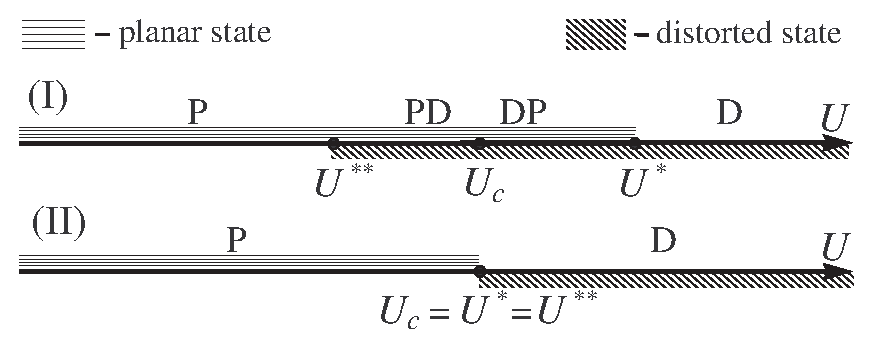
\includegraphics[width=12cm]{UU1d3a.eps}
	\caption{Иллюстрация разрывного (I) и непрерывного (II) переходов Фредерикса для $U > 0$.
		(I): Области устойчивости искажённой (D) структуры, $U>U^{**}$, и неискажённой (P) структуры, $U<U^{*}$.
		На интервале, обозначенном PD, $U^{**}<U<U_c$, искажённая структура метастабильна, а на интервале DP, $U_c < U < U^{*}$, метастабильна планарная геликоидальная структура.
		(II):  Области устойчивости для искажённой, $U > U_c$, и неискажённой структуры, $U < U_c$.}
	\label{pic-U*U**Uc_otline}
\end{figure}

Для того, чтобы изучить, как влияет флексоэлектрическая поляризация на переход Фредерикса, были рассчитаны пороговые напряжения $U^{**}$, $U_c$, $U^{*}$ для различных значений усреднённого флексоэлектрического коэффициента $\bar{e}$.
Отметим, что учёт флексоэлектричества привёл к тому, что значения напряжений $U^{**}$, $U^*$ и $U_c$ стали различными для  $U>0$ и $U<0$, если константы сцепления с подложкой различны, $W_\theta^{(1)}\not=W_\theta^{(2)}$.
Значения материальных констант были взяты такими же, как и в~~\cite{VAR2013}: $K_{11}=0.42\times 10^{-6}$~дин, $K_{22}=0.23\times 10^{-6}$~дин, $K_{33}=0.53\times 10^{-6}$~дин,  $q_0=500$~$\text{cm}^{-1}$, $L=60$~$\mu\text{m}$, $W_\theta^{(1)}=2.5\times 10^{-3}$~эрг/см$^2$, $W_\theta^{(2)}=0.5\times 10^{-3}$~эрг/см$^2$,  $W_\phi^{(1)}=2.5\times 10^{-4}$~эрг/см$^2$, $W_\phi^{(2)}=1.0\times 10^{-4}$~эрг/см$^2$, $\varepsilon_\bot=7.2$, $\varepsilon_\|=16.2$.
\todo{В дальнейшем будем называть этот набор параметров стандартным.}
Выбранные значения параметров $q_0$ и $L$ соответствуют супертвист-ячейке ЖК с полной закруткой $q_0L = 3>\pi/2$.
Кроме того, значения констант сцепления с подложкой выбраны сильно различающимися, чтобы продемонстрировать влияние такой асимметрии границ.
На Рис.~\ref{pic-U_from_e_pos} представлена рассчитанная "фазовая диаграмма" в координатах ($\bar{e}$, $U$) для обоих направлений электрического поля.
\begin{figure}%[bht]
	\centering
	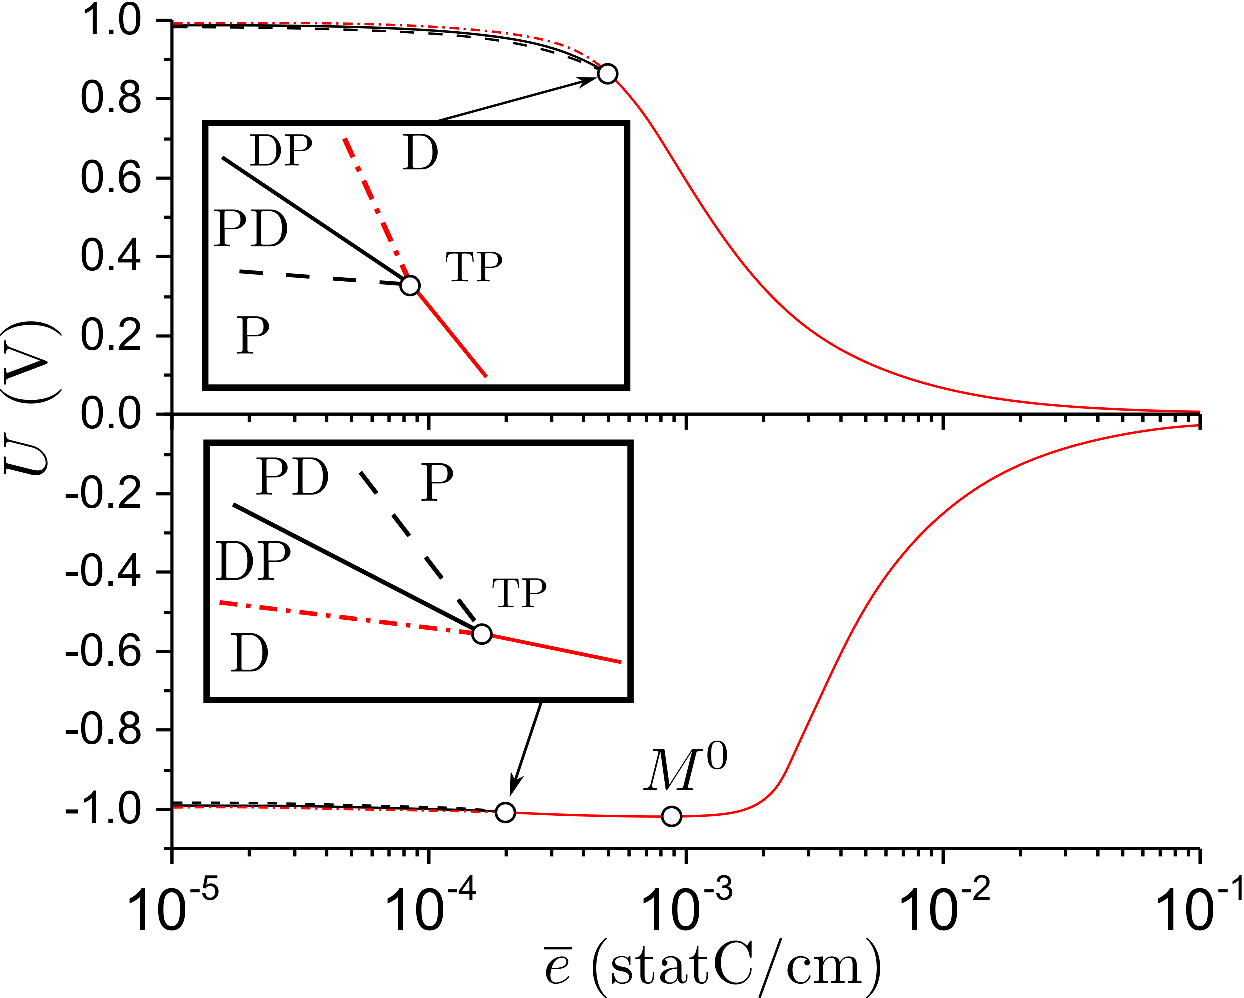
\includegraphics[width=15cm]{Graph7colorB.eps}
	\caption{Фазовая диаграмма.
		Напряжения $U^*$, $U_c$ и $U^{**}$ как функции усреднённого флексоэлектрического коэффициента $\bar{e}$: пунктирная линия -- $U^{**}$, сплошная линия -- $U_c$, штрихпунктирная линия -- $U^{*}$.
		Области стабильности и метастабильности обозначены на вставках.
		Трикритические точки обозначены как TP, другие обозначения совпадают с таковыми на Рис.~\ref{pic-U*U**Uc_otline}.
		Правее трикритической точки TP линии $U^*$, $U_c$ и $U^{**}$ совпадают.}
	\label{pic-U_from_e_pos}
\end{figure}
Интересно отметить, что в случае $U>0$ пороговые напряжения $U^*$, $U_c$ and $U^{**}$ монотонно убывают с ростом $\bar{e}$, то есть в этом случае флексоэлектричество способствует переходу Фредерикса.
Однако эти зависимости оказываются немонотонными для $U < 0$ (точка минимума обозначена как $M^0$).
В случае симметричных границ, то есть, когда $W^{(1)}_\theta = W^{(2)}_\theta$ и $W^{(1)}_\varphi = W^{(2)}_\varphi$, кривые $U^*$, $U_c$ и $U^{**}$ симметричны относительно $U = 0$.
С ростом $\bar{e}$ переход Фредерикса меняет свой род: он оказывается разрывным для небольших $\bar{e}$ и непрерывным для больших $\bar{e}$.
Такая смена рода перехода происходит в трикритической точке TP, окрестность которой схематично показана во вставке на Рис.~\ref{pic-U_from_e_pos}.

\subsubsection{Равновесные ориентационные структуры}

На Рис.~\ref{Fig_profles_sym} представлены равновесные профили $\theta(z)$ и $\phi(z)$, рассчитанные при попарно одинаковых константах сцепления с подложкой (прочие параметры совпадают со стандартным набором).
\begin{figure}%[thb]
	\hspace{0cm}
	\centering
	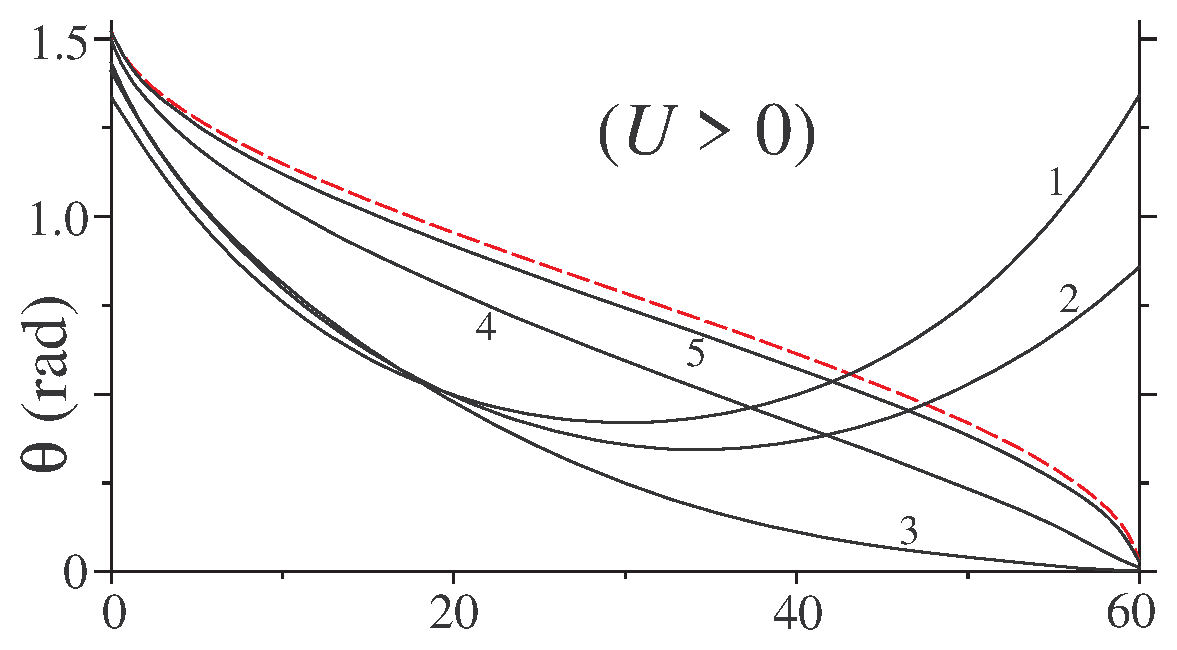
\includegraphics[width=8.5cm]{symm_all_6curvesNoReflect1a.eps}
	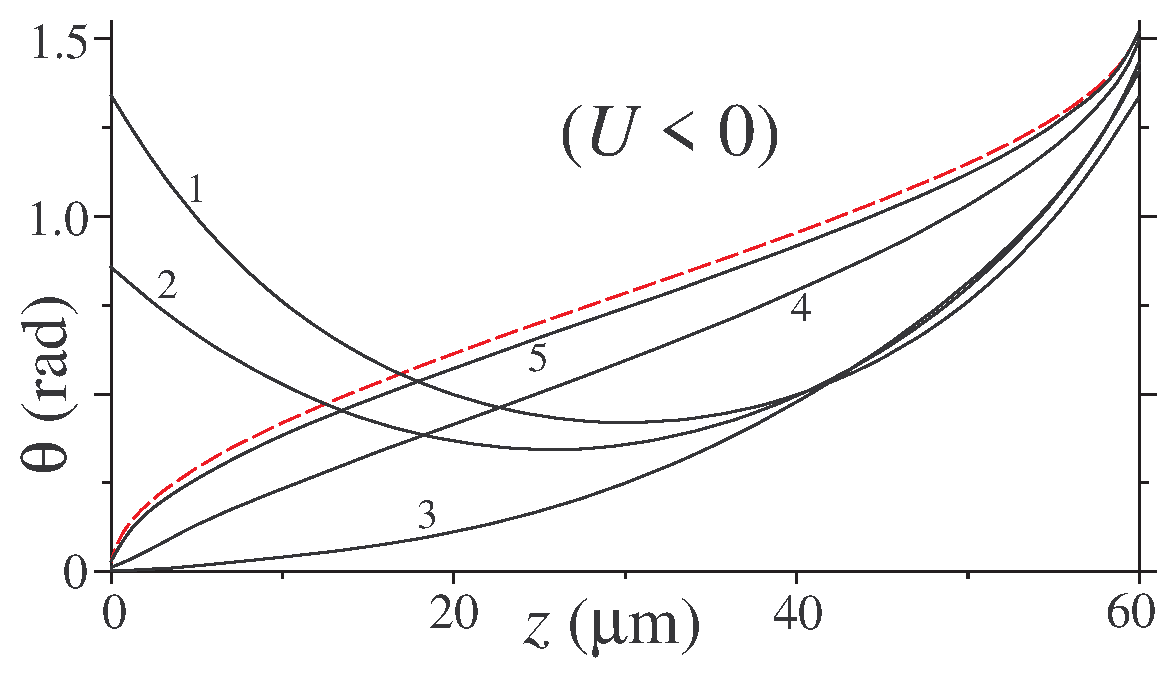
\includegraphics[width=8.5cm]{symm_all_6curvesReflect1.eps}
	\caption{Рассчитанные равновесные профили $\theta(z)$ при $U = \pm 1.2$~В для случая симметричных модулей сцепления с границами: $W_\theta^{(1)}=W_\theta^{(2)}=1.5\times 10^{-3}$~эрг/см$^2$, $W_\phi^{(1)}=W_\phi^{(2)}=1.5\times 10^{-4}$~эрг/см$^2$; остальные параметры стандартные.
	Номера профилей и соответствующие им значения $\bar{e}$ совпадают с таковыми на Рис.~\ref{Fig_profles_nonsym}, кроме графика 2, построенного для $\bar{e} = 5\times 10^{-4}$~Фр/см.
	Красные пунктирные профили рассчитаны по формуле~\eqref{eq_cos2_lin1}.}
	\label{Fig_profles_sym}
\end{figure}
Важно отметить, что именно благодаря флексоэлектричеству профили $\theta(z)$ оказываются асимметричными относительно $z=L/2$.
Это можно пояснить на примере графиков для достаточно больших значений $\bar{e}$.
Из формулы для энергии взаимодействия ХЖК с электрическим полем~\eqref{eq_F_f_final1} видно, что в этом случае основной вклад в свободную энергию даёт слагаемое, содержащее $\bar{e}^2$.
Его можно записать в следующем виде:
\begin{equation}
2\pi S_{\!\bot} \bar{e}^2\int_{0}^{L}\frac{(\sin 2\theta \,\theta'-JJ_1)^2}{{\EE}(\theta)}dz.
\end{equation}
Отметим, что оно принимает минимальное (нулевое) значение, когда $\sin2\theta \, \theta'-JJ_1=0$.
Это интегро-дифференциальное уравнение имеет точное рещение:
\begin{equation}\label{eq_cos2_lin}
\cos^2 \theta(z) =az+b,
\end{equation}
где $a$ и $b$ -- произвольные константы.
При таком $\theta(z)$ член в~\eqref{eq_F_f_final1}, содержащий $\bar{e}^2$, близок к нулю.
Следовательно, главный вклад в $\FF_\mathrm{E}$ даётся вторым слагаемым в~\eqref{eq_F_f_final1}, $S_{\!\bot} \bar{e}U JJ_1\approx S_{\!\bot} \bar{e}U \sin2\theta\, \theta'= -S_{\!\bot} \bar{e}U (\cos^2\theta)'\approx -S_{\!\bot} \bar{e}Ua$.
Для того, чтобы теперь минимизировать  $\FF_\mathrm{E}$, нужно сделать максимальным значение выражения $a\sgn(\bar{e}U)$.
Отметим, что $aL = \cos^2{\theta(L)} - \cos^2{\theta(0)}$, а значит, минимум $\FF_\mathrm{E}$ достигается, когда $\theta(0)\approx\pi/2$, $\theta(L)\approx 0$ для $\bar{e}U>0$ и когда $\theta(0)\approx 0$, $\theta(L)\approx\pi/2$ для $\bar{e}U<0$.
Следовательно, в соответствии с формулами~\eqref{eq_cos2_lin} и \eqref{eq:phi_profile}, при достаточно больших значениях $\bar{e}$ профили углов имеют вид
\begin{equation}\label{eq_cos2_lin1}
\theta(z)\simeq
\begin{cases}
\arccos\sqrt{z/L}, & \bar{e}U>0,\\
\arccos\sqrt{1-z/L}, & \bar{e}U<0,
\end{cases}
\end{equation}
\begin{equation}\label{eq:phi_profile1}
\varphi(z) \simeq
\begin{cases}
\phi_0^{(1)} + \frac{q_0 L}{\zeta} \ln\left( 1 + \zeta\frac{z}{L} \right), & \bar{e}U>0,\\
\phi_0^{(2)} - \frac{q_0 L}{\zeta} \ln\left(1 + \zeta\left(1 - \frac{z}{L}\right)\right), & \bar{e}U<0,
\end{cases}
\end{equation}
где $\zeta = (K_{33} - K_{22})/K_{22}$.
Заметим, что первая формула в~\eqref{eq:phi_profile1} неприменима в окрестности точки $z = L$, а вторая -- в окрестности $z = 0$.
Для того, чтобы корректно описать зависимость $\phi(z)$ в окрестности этих точек, необходимо учитывать в~\eqref{eq_cos2_lin1} малые поправки $\sim 1/\bar{e}$.

Такой же эффект наблюдается и для профилей $\theta(z)$ и $\phi(z)$, рассчитанных для различных $\bar{e}$ и несимметричных констант сцепления с подложкой (в данном случае значения всех материальных параметры совпадают с указанными в предыдущем разделе). Данные профили представлены на Рис.~\ref{Fig_profles_nonsym}.
\begin{figure}%[bth]
%	\hspace{0cm}
	\centering
	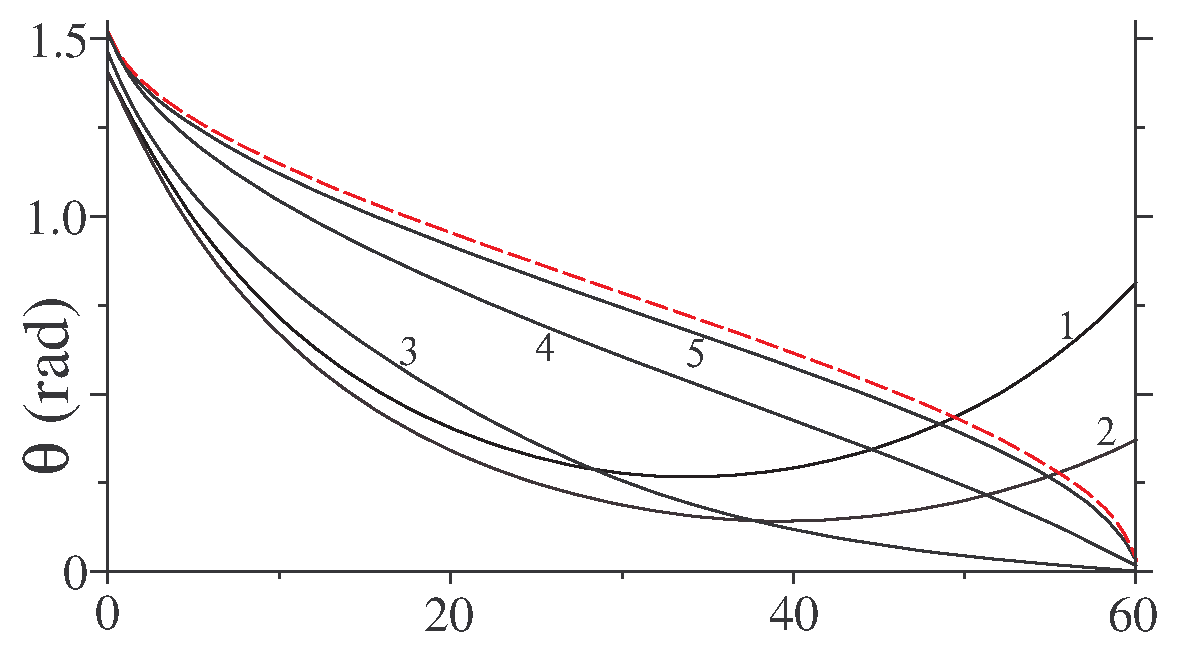
\includegraphics[width=8.5cm]{asymm_theta_6curves1.eps}
	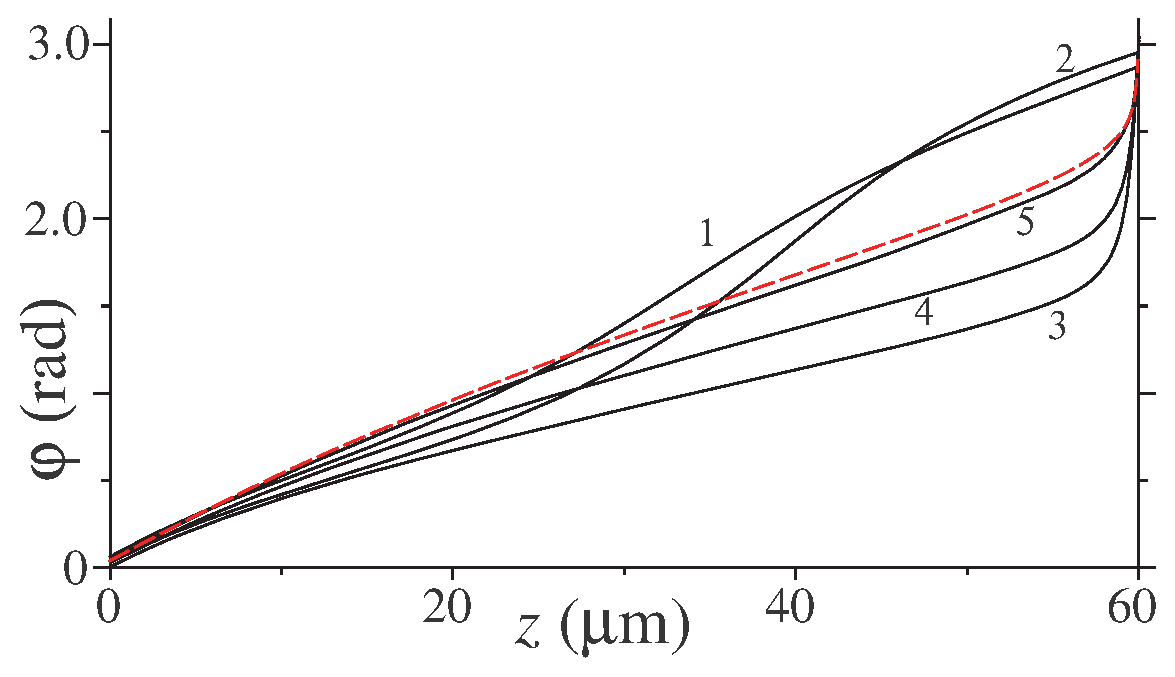
\includegraphics[width=8.5cm]{asymm_phi_6curves1.eps}
	\caption{Равновесные профили $\theta(z)$ и $\phi(z)$, рассчитанные при $U = 1.2$~V. 
		Кривые 1 соответствуют ЖК без флексоэлектричества, $\bar{e}=0$; кривые 2 соответствуют $\bar{e}=10^{-4}$~Фр/см, кривые 3 соответствуют $\bar{e}=10^{-3}$~Фр/см, кривые 4 соответствуют $\bar{e}=3\times 10^{-3}$~Фр/см, а кривые 5 соответствуют $\bar{e}=10^{-2}$~Фр/см. Красные пунктирные линии соответствуют профилям, рассчитанным по формулам~\eqref{eq_cos2_lin1} and~\eqref{eq:phi_profile1}.}
	\label{Fig_profles_nonsym}
\end{figure}
Видно, что и в этом случае при достаточно больших значениях $\bar{e}$ зависимость $\theta(z)$ стремится к рассчитанной выше~\label{eq_cos2_lin1}.

Покажем, как влияет род перехода Фредерикса на ориентационную структуру в ячейке сразу после перехода.
\begin{figure}%[htb]
	\hspace{0cm}
	\centering
	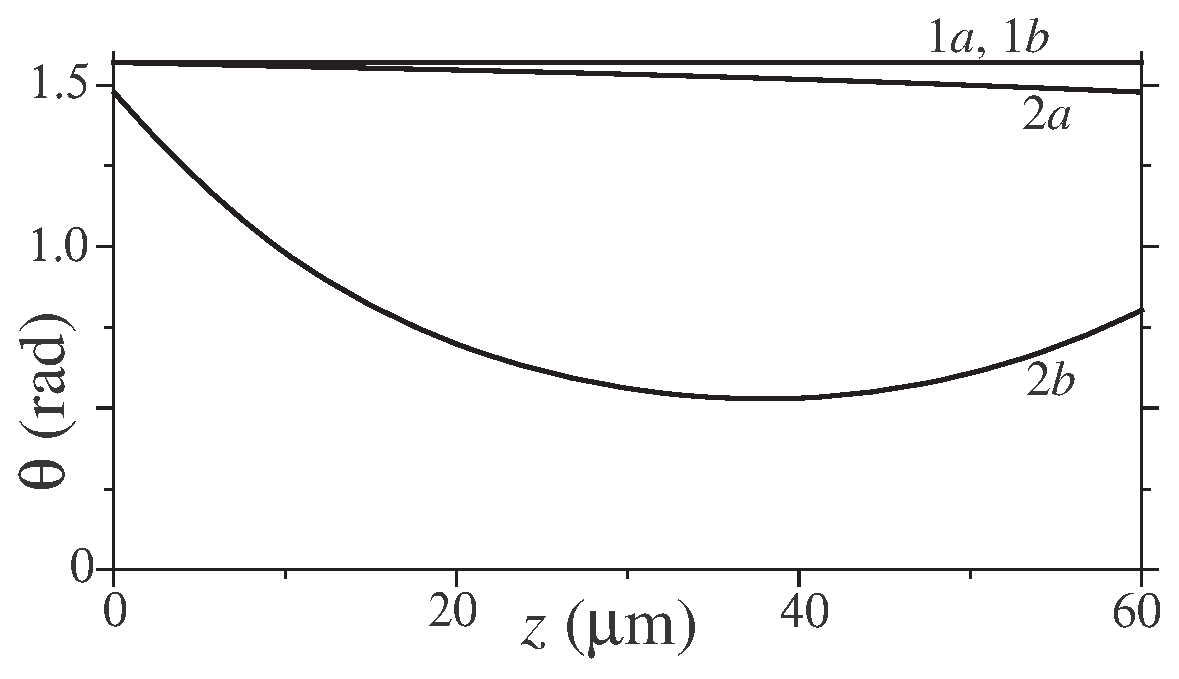
\includegraphics[width=10cm]{1_005Uc_profiles1.eps}
	\caption{Профили $\theta(z)$ для случая непрерывного (a) и разрывного (b) переходов.
		Совпадающие линии профили 1a и 1b соответствуют планарной геликоидальной структуре ($U = 0.999 U_c$), а профили с номером 2 соответствуют искажённым структурам ($U = 1.005 U_c$).
		Для профилей в случае "a": $\bar{e} = 8\times 10^{-4}\text{~Фр/см}<\bar{e}^\text{TP}$, а в случае "b": $\bar{e} = 2\times 10^{-4}\text{~Фр/см}>\bar{e}^\text{TP}$, где $\bar{e}^\mathrm{TP}=5.132\times10^{-4}\text{~Фр/см}$.
		Пороговые значения напряжений составляют: (a) $U_c=0.6926$~В, (b)  $U_c=0.9396$~В.
		Остальные материальные параметры соответствуют таковым на Рис.~\ref{Fig_profles_nonsym}. }
	\label{figCont_Discont_profiles}
\end{figure}
Из Рис.~\ref{pic-U_from_e_pos} можно видеть, что область сосуществования различных ориентационных структур очень узкая при выбранных значениях материальных констант.
%С целью самопроверки
Были рассчитаны профили $\theta(z)$ для двух различных значений $\bar{e}$, больше и меньше $\bar{e}^\text{TP}$ при различных значениях приложенного напряжения.
При напряжении $U < U_c$ структура системы остаётся планарной геликоидальной.
Затем была рассчитана ориентационная структура при напряжении, большем критического $U_c$ на $0.5\%$.
Было обнаружено, что имеется значительное различие между профилями $\theta(z)$ в случае разрывного и непрерывного переходов (Рис.~\ref{figCont_Discont_profiles}).
Следовательно, разрывность перехода значительно меняет ориентационную структуру даже если разница между $U^*$ и $U^{**}$ очень мала.
           % Глава 2
%\chapter{Аналитическое изучение устойчивости планарной геликоидальной структуры.}\label{ch:ch3}

Планарная геликоидальная структура описывается парой угловых функций $\theta_0(z) = \pi/2$, $\phi_0(z) = q_0 z$, $z\in[0,\,L]$.
Для определения устойчивости этой структуры нужно изучить вторую вариацию свободной энергии на этой структуре, $\delta^2\FF_\mathrm{tot}(\theta_0,\phi_0)$. 
Вторая вариация свободной энергии в отсутствие флексоэлектрической поляризации уже была найдена в работе~\cite{VAR2013}:
\begin{multline}\label{eq:F2_on_planar_helicoidal}
\left.\delta^2\FF_{\text{tot}}\right|_{\bar{e}=0}
=\frac{S_{\!\bot}}{2}\bigg[\int_{0}^{L}
\left(K_{11}(\delta\theta')^2+M\delta\theta^2+K_{22}(\delta\phi')^2\right)\, dz +\\
+\sum_{\alpha=1,2}W_\theta^{(\alpha)}\delta\theta^2(l_\alpha)
+\sum_{\alpha=1,2}W_\phi^{(\alpha)}\delta\phi^2(l_\alpha)\bigg],
\end{multline}
где
\begin{equation}
M = K_{33}q_0^2 - \varepsilon_a U^2/(4\pi L^2).
\end{equation}
Так как $J_1\big|_{\theta = \theta_0}=0$ и $\delta J_1\big|_{\theta = \theta_0}=0$, то вклад во вторую вариацию свободной энергии, обусловленный флексоэлектрической поляризацией, даётся выражением
\begin{equation}\label{get_d2Flex}
\delta^2\FF_{\mathrm{flex}}
=-S_{\!\bot}\bar{e} (U/L) \delta\theta^2\Big|_0^L.
\end{equation}
Следовательно, вторая вариация свободной энергии $\delta^2\FF_\mathrm{tot}=\left.\delta^2\FF_{\text{tot}}\right|_{\bar{e}=0} + \delta^2\FF_{\mathrm{flex}}$ оказывается суммой двух независимых вариаций по углам $\theta$ и $\phi$.
При этом часть, зависящая от вариации $\phi$, положительно определена, так как $K_{22}>0$ and $W^{(1,2)}_\varphi>0$.
Таким образом, устойчивость планарной геликоидальной струтктуры определяется только членами, зависящими от вариации $\theta$:

\begin{equation}\label{d2F_theta}
\delta^2 \FF_\theta =
\frac{S_{\!\bot}}{2}\int_{0}^{L}\left(K_{11}(\delta\theta')^2 + M(\delta\theta)^2\right) dz + \frac{S_{\!\bot}}{2}\sum_{\alpha=1,2}
\EuScript{W}^{(\alpha)}
\delta\theta^2(l_\alpha),
\end{equation}
где
\begin{equation}\label{W_renorm}
\EuScript{W}^{(\alpha)}=W_\theta^{(\alpha)} - 2(-1)^\alpha\bar{e} U/L.
\end{equation}
Вклад флексоэлектрической поляризации во вторую вариацию свободной энергии $\delta^2\FF_\text{tot}$ сводится к ренормированию модулей сцепления с поверхностью, $W_\theta^{(\alpha)}\rightarrow \EuScript{W}^{(\alpha)}$.
Следует отметить, что один из эффективных модулей зацепления $\EuScript{W}^{(\alpha)}$ с ростом приложенного напряжения $U$ увеличивается и остаётся положительным, в то время как другой уменьшается и при достаточно больших значениях $U$ становится отрицательным.
Введём следующие обозначения:
\begin{equation}\label{Wtheta_eff_pm}
\EuScript{W}^{+} =
\begin{cases}
\EuScript{W}^{(1)},&\mbox{if } U >0,\\
\EuScript{W}^{(2)},& \mbox{if } U<0,
\end{cases}\quad
\EuScript{W}^{-} =
\begin{cases}
\EuScript{W}^{(2)},& \mbox{if } U >0,\\
\EuScript{W}^{(1)},& \mbox{if } U<0.
\end{cases}
\end{equation}
Как следует из выражения~\eqref{d2F_theta}, планарная геликоидальная структура может стать неустойчивой только если хотя бы один из параметров $\{M, \EuScript{W}^{-}\}$ отрицателен.
В дальнейшем в этой главе ограничимся рассмотрением случая положительной анизотропии диэлектрической проницаемости, $\epsilon_a > 0$.
Таким образом, неустойчивось возможна в следующих ситуациях:
\begin{equation}\label{3_instability_conditions_W}
\begin{aligned}
\centering
\mathrm{I}. &&M < 0,\quad & \EuScript{W}^{-} \geq  0,\\
\mathrm{II}. && M < 0,\quad &\EuScript{W}^{-} < 0,\\
\mathrm{III}. && M \geq 0,\quad &\EuScript{W}^{-} < 0.\\
\end{aligned}
\end{equation}
Условия~\eqref{3_instability_conditions_W} можно записать в виде неравенств для напряжения $U$:
\begin{equation}
\begin{split}
&\mathrm{I}.\quad U_e< \left|U\right| \leq U_\mathrm{flex},\\
&\mathrm{II}.\; \left|U\right|> \max( U_e, U_\mathrm{flex}),\\
&\mathrm{III}.\; U_\mathrm{flex}< \left|U\right| \leq U_e.
\end{split}
\label{eq:conditions_for_voltages}
\end{equation}
Здесь введены обозначения:
\begin{equation}\label{UfrUfl}
U_e =2 q_0 L \sqrt{\frac{\pi K_{33}}{\varepsilon_a}}, \;
U_\mathrm{flex}=
\frac{L}{2\bar{e}}
\begin{cases}
W_\theta^{(2)},&\!\! \text{if } U >0,\\
W_\theta^{(1)},&\!\!\text{if } U<0.
\end{cases}
\end{equation}
Области на плоскости $(\bar{e},\,U)$, соответствующие этим неравенствам, изображены на Рис.~\ref{pic:Zones}.

Представим $\delta \theta(z)$ в виде суммы двух слагаемых:
\begin{equation}\label{thetamupsi}
\delta\theta(z) = \delta\psi(z) + \delta\mu(z),
\end{equation}
где
\begin{equation}\label{mu0=muL=0}
\delta\mu(0) = \delta\mu(L) = 0.
\end{equation}
\todo{Функция $\delta\psi(z)=\delta\psi(z,\delta_1,\delta_2)$ выбрана как решение следующего дифференциального уравнения с граничными условиями:}
\begin{equation}
\begin{cases}
K_{11} \delta\psi''(z) - M\delta\psi(z) = 0,\\
\delta\psi(0) = \delta_1,\ \delta\psi(L) = \delta_2.
\end{cases}
\label{eq:diff_system}
\end{equation}
Такой выбор $\delta\mu(z)$ и $\delta\psi(z)$ даёт возможность разделить интегральный член в~\eqref{d2F_theta}, на два слагаемых, по отдельности зависящих от этих функций; выполнение первого условия в~\eqref{eq:diff_system} позволяет исключить ``перекрёстный член'' после подстановки $\delta\psi(z)$ и $\delta\mu(z)$ в~\eqref{d2F_theta}.

Решение уравнения~\eqref{eq:diff_system} может быть представлено в следующем виде:
\begin{equation}\label{psi=}
\delta\psi =
\begin{cases}
\displaystyle\delta_1\frac{\sin \xi(L-z)}{\sin\xi L}+\delta_2\frac{\sin\xi z}{\sin\xi L},&\quad M < 0,\hspace{-4mm} \\
\displaystyle\delta_1 (L - {z})/{L} + \delta_2{z}/{L},\hspace{-4mm} &\quad M = 0,\\
\displaystyle\delta_1\frac{\sinh \xi(L-z)}{\sinh\xi L}+\delta_2\frac{\sinh\xi z}{\sinh\xi L},\hspace{-4mm} &\quad M > 0,\\
\end{cases}
\end{equation}
где обратная длина $\xi$ определяется как
\begin{equation}\label{xi=}
\xi = \sqrt{\left|M\right|K_{11}^{-1}} = \sqrt{\left|K_{33}q_0^2-\varepsilon_a U^2/(4\pi L^2)\right|K_{11}^{-1}}.
\end{equation}
Разделяя $\delta\theta$ на два слачаемых, даваемых выражениями~\eqref{thetamupsi} и~\eqref{psi=}, представим $\delta^2\FF_\theta$ в виде суммы двух независимых квадратичных форм
\begin{equation}
\delta^2 \FF_\theta =\frac{1}{2}S_{\!\bot}( Q_\psi + Q_\mu),
\label{eq:separation_into_two_modes}
\end{equation}
где
\begin{eqnarray}\label{Qdelta0}
\hspace{-7mm}&&Q_\psi= \int_{0}^{L}\left(K_{11}\delta\psi'^2(z)+M\delta\psi^2(z)\right)\mathrm{d}z
+\!\sum_{\alpha=1,2}\EuScript{W}^{(\alpha)}\delta_\alpha^2,\\
\hspace{-7mm}&&Q_\mu=\int_{0}^{L}\left(K_{11}(\delta\mu')^2+M(\delta\mu)^2\right)\mathrm{d}z.\label{Qmu}
\end{eqnarray}
Стоит отметить, что только $Q_\psi$ зависит от искажений на границе $\delta_{1,2}$.
Идея такого разделения вариации на часть, зависящую от вариации функции в объёме и часть, зависящую от, в том числе, граничных вариаций, впервые была применена Фейнманом~\cite{Feynman}.
Сейчас эта идея широко используется при описании ячеек ЖК~\cite{VRR2001, Kiselev2004, VAR2013}.
Так как $K_{11}>0$, квадратичная форма $Q_\mu$ определена положительно, если $M\geq 0$ ($|U|\leq U_e$).
Однако условие $M \geq 0$ можно ослабить, так как вариации $\delta\mu$ и $\delta\mu'$ связаны.
Для этого представи $\mu(z)$ в виде ряда Фурье на интервале $[0; \, L]$.
Принимая во внимание граничные условия~\eqref{mu0=muL=0}, удобно записать ряд Фурье только по синусам
\begin{equation}\label{sine_expansion}
\mu(z)=\sum\limits_{m=1}^{\infty}c_m \sin{\frac{\pi m z}{L}}\,,
\end{equation}
так как каждое слагаемое в~\eqref{sine_expansion} обращается в ноль при $z=0$ и $z=L$. 
Подставляя разложение~\eqref{sine_expansion} в~\eqref{Qmu}, получаем
\begin{equation}\label{4.1.2.6n}
Q_\mu=\frac{L}{4}\sum\limits_{m=1}^{\infty}
c_m^2\left[K_{11}\left(\frac{\pi m}{L}\right)^2+M\right]\,.
\end{equation}
Условие положительной определённости $Q_\mu$ эквивалентно положительности всех коэффициентов 
\begin{equation}\label{coeffs_at_cm}
K_{11}\left(\frac{\pi m}{L}\right)^2 + M,\ m \geq 1,
\end{equation}
так как $c_m$ могут принимать произвольные значения.
Заметим, что значения коэффициентов~\eqref{coeffs_at_cm} растут с увеличением $m$, так как $K_{11} > 0$.
Таким образом, положительность всех коэффициентов определяется положительностью первого из них:
\begin{equation*}
\left(\frac{\pi}{L}\right)^2K_{11} + M > 0,
\end{equation*}
что, учитывая определение $\xi$~\eqref{xi=}, позволяет записать~\autocite{VAR2013}
\begin{equation}\label{xiL<pi}
\xi L < \pi.
\end{equation}
Подставляя~\eqref{psi=} в~\eqref{Qdelta0}, получаем
\begin{equation}\label{eq:Q_psi_final}
Q_\psi=
\begin{cases}
\begin{aligned}\sum\limits_{\alpha=1,2}\left(K_{11}\xi \cot{\xi L}+\EuScript{W}^{(\alpha)}\right) \delta_\alpha^2 - \\
\phantom{\sum_{a}}
- 2K_{11}(\xi/\sin\xi L)\delta_1\delta_2,
\end{aligned}&\text{при } M<0,\\
\begin{aligned}\sum\limits_{\alpha=1,2}\left(K_{11}/L
+\EuScript{W}^{(\alpha)}\right) \delta_\alpha^2 - \qquad\\
\phantom{\sum_{a}}-  2(K_{11}/L)\delta_1\delta_2,
\end{aligned}&\text{при } M=0,\\
\begin{aligned}
\sum\limits_{\alpha=1,2}\left(K_{11}\xi \coth{\xi L}+\EuScript{W}^{(\alpha)}\right) \delta_\alpha^2 - \\
- 2K_{11} (\xi/\sinh\xi L)\delta_1\delta_2,
\end{aligned}& \text{при } M>0.
\end{cases}
\end{equation}
Используя критерий Сильвестра для $Q_\psi$ и учитывая неравенство~\eqref{xiL<pi}, получаем условия устойчивости планарной геликоидльной структуры ХЖК:
\begin{subequations}\label{eq:ineq_all_M_final}
\begin{align}
&\text{при}\; |U|>U_e:\,
\begin{cases}
{ 0< t} < \pi,\\
w^{+}+t\cot t>0,\\
w^{(1)}w^{(2)}+2\bar{w} t \cot {t}> t^2,
\end{cases}\label{eq:ineq_M<0_final_a}\\
&\text{при}\; |U|=U_e:\,
\begin{cases}
t = 0,\\
w^{+}+1>0,\\
w^{(1)}w^{(2)}+2\bar{w}> 0,
\end{cases}\label{eq:ineq_M=0_final_b}\\
&\text{при}\; |U|<U_e:\,
\begin{cases}
{ t>0,}\\
w^{+}+ t\coth t>0,\\
w^{(1)}w^{(2)}+2\bar{w}  t \coth t>- t^2,
\end{cases}\label{eq:ineq_M>0_final_c}
\end{align}
\end{subequations}
где введены безразмерные параметры $t = \xi L$, $w^{+}={\EuScript{W}^{+} L}/{K_{11}}$, $w^{(\alpha)}={\EuScript{W}^{(\alpha)} L}/{K_{11}}$, и $\bar{w}=({W}^{(1)}_\theta+{W}^{(2)}_\theta)L/2K_{11}$.
Покажем, что каждая из систем неравенств~\eqref{eq:ineq_all_M_final} может быть сведена к одному неравенству.
Рассмотрим систему неравенств~\eqref{eq:ineq_M<0_final_a} и сравним первое и второе.
Для этого построим график функции $f(t) = t \cot{t} + w^{+}$ на интервале $t\in(0,\, \pi)$ (см. Рис.~\ref{pic:graphs_for_inequalities}).
Видно, что решение неравенства $f(t) > 0$ -- интервал $(0, t')$, где $t'$ -- корень уравнения $f(t) = 0$, причём $t'\in(\pi/2,\, \pi)$.
Таким образом, выполнение второго неравенства гарантирует выполнение первого (при этом условие $t>0$ естественным образом следует из определения $t$).
\begin{figure}\label{pic:graphs_for_inequalities}
	\centering
	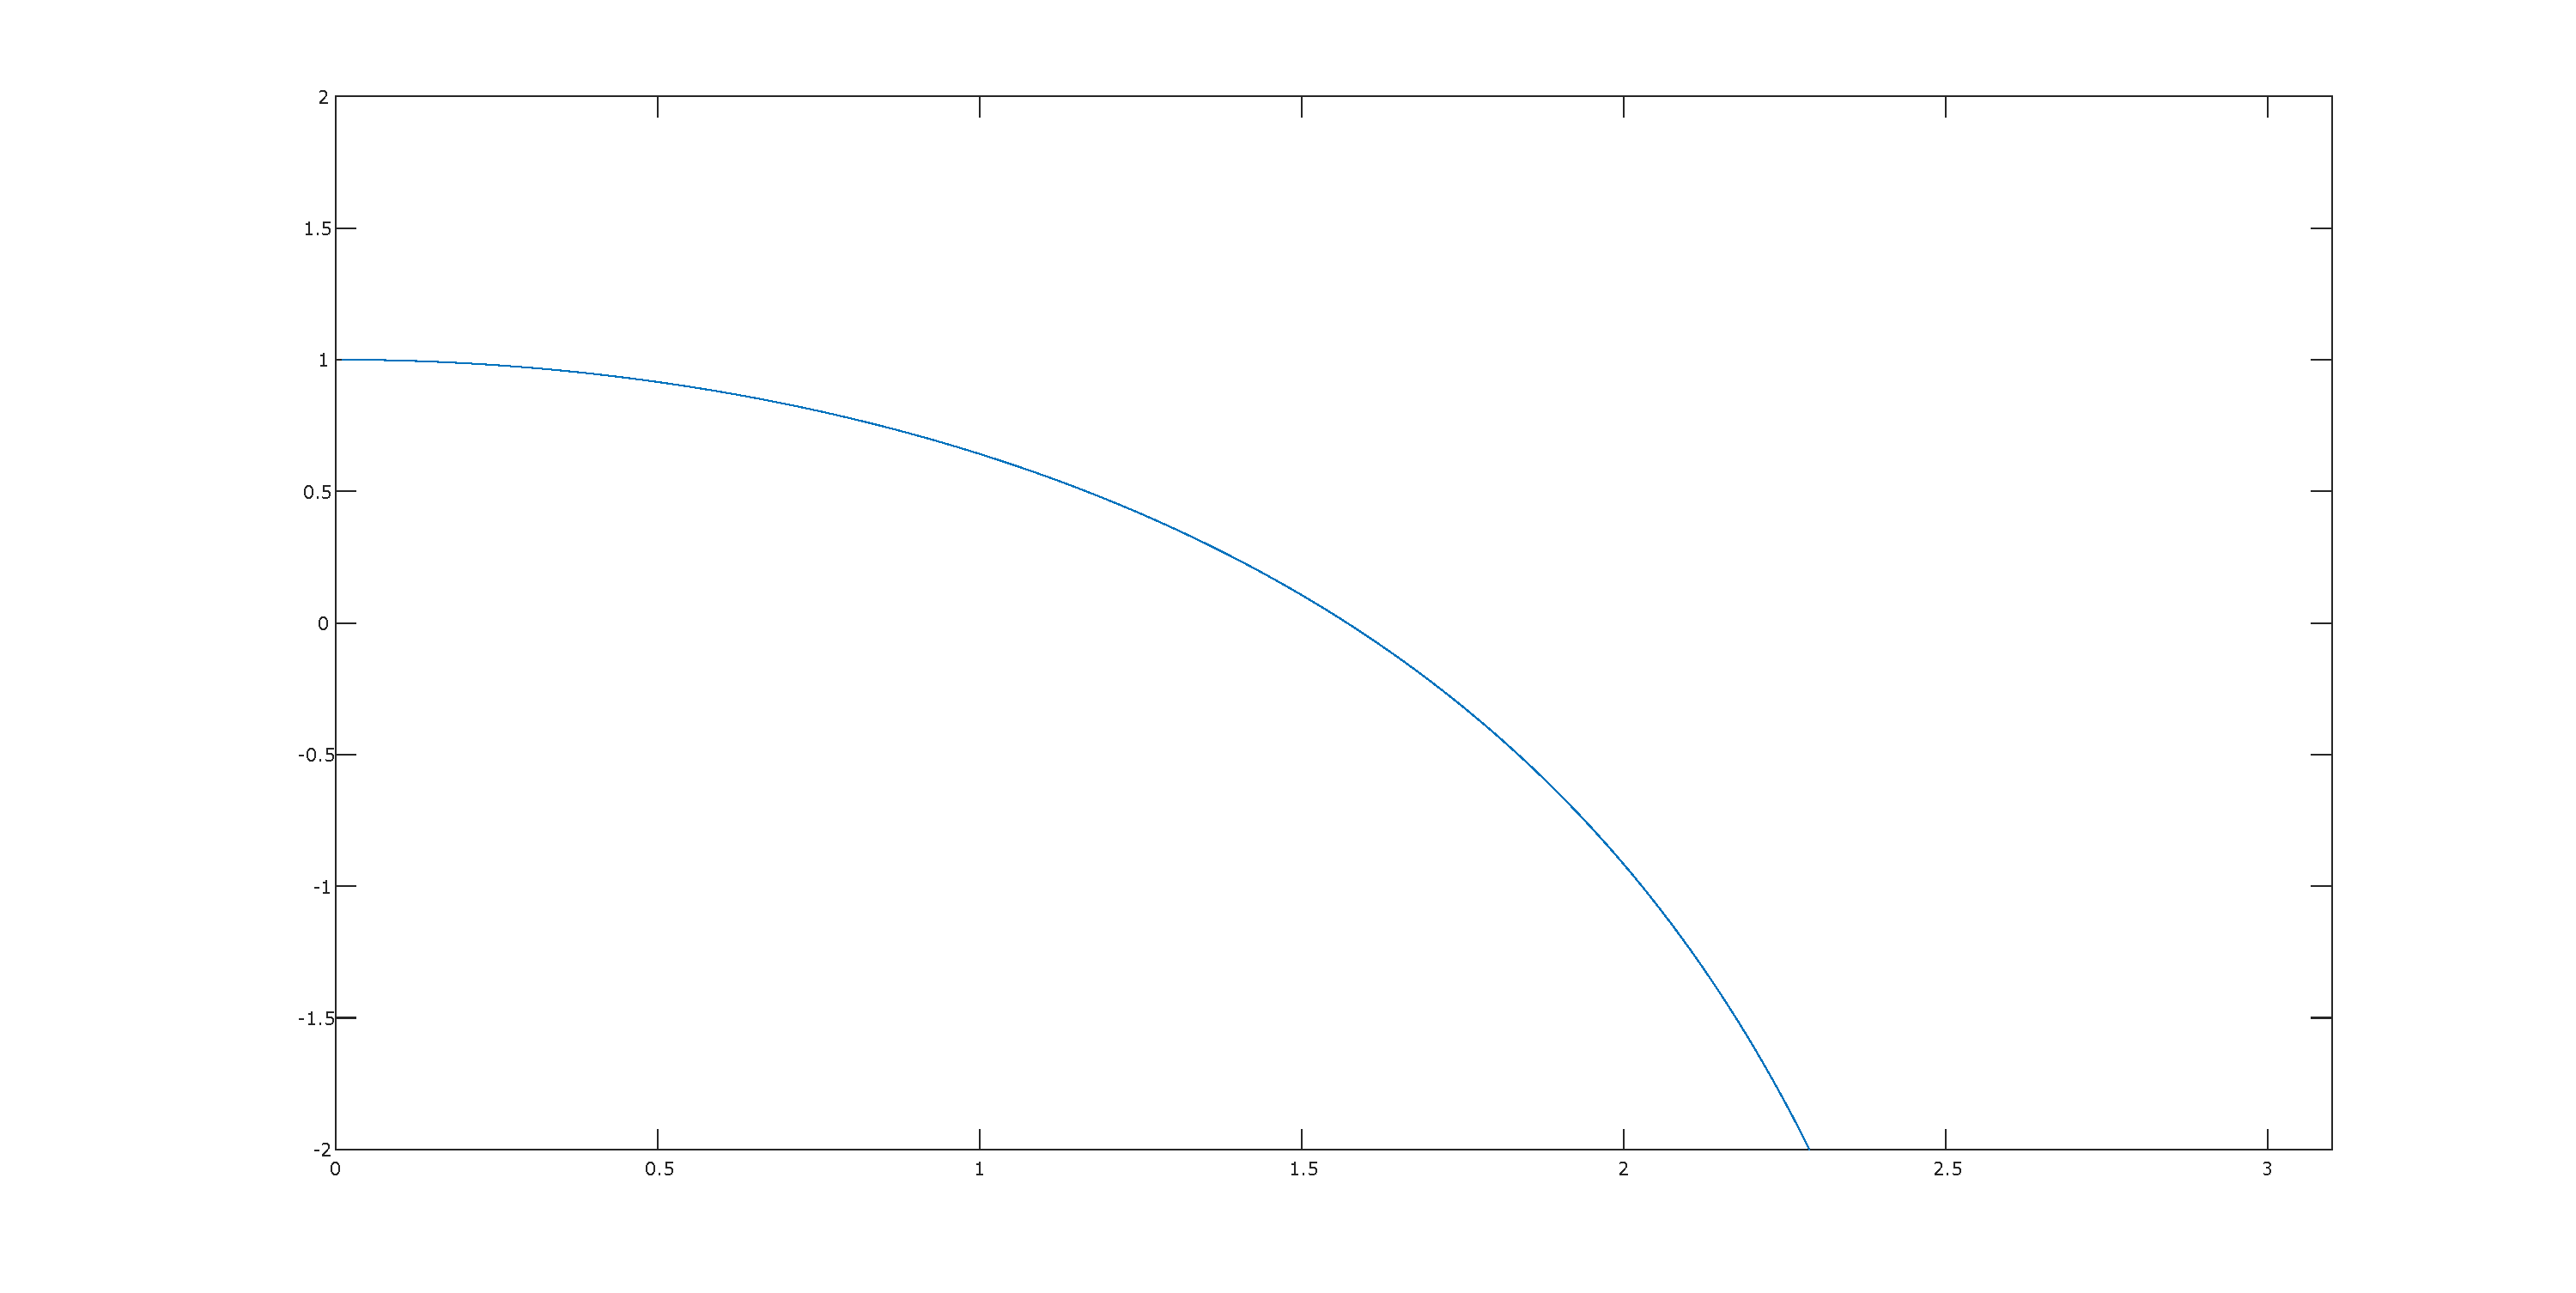
\includegraphics[width = 10cm]{drawing.eps}
	\caption{Some Caption}
\end{figure}
Для сравнения второго неравенства с третьим умножим второе на $2\bar{w}$, получим:
\begin{equation}
w^{+}w^{-} + (w^{+})^2 + 2\bar{w} t\cot{t} > 0.
\end{equation}
Обозначая $F(t) = w^{+}w^{-} + 2\bar{w} t\cot{t}$, можно переписать второе и третье неравенства в следующем виде:
\begin{equation}
\begin{cases}
(w^{+})^2 + F(t) > 0\\
F(t) - t^2 > 0.
\end{cases}
\end{equation}
Видно, что при выполнении последнего неравенства (соответственно, третьего в~\eqref{eq:ineq_M<0_final_a}) второе также выполняется.
Далее, нетрудно видеть, что первое и второе неравенства в системах~\eqref{eq:ineq_M=0_final_b} и~\eqref{eq:ineq_M>0_final_c} выполняются при любых возможных значениях $t$ и $w^{+}$.
Таким образом, мы показали, что последнее неравенство в каждой из систем в~\eqref{eq:ineq_all_M_final} определяющее, а значит, является критерием устойчивости:
\begin{equation}\label{stab_cond_final}
\begin{aligned}
&w^{(1)}w^{(2)}+2\bar{w} t \cot{t}- t^2>0,\hspace{-2mm} & \text{if}\; |U|>U_e,\\
&w^{(1)}w^{(2)}+2\bar{w} > 0, \hspace{-2mm} &\text{if}\; |U|=U_e,\\
&w^{(1)}w^{(2)}+2\bar{w}   t \coth t+ t^2>0, \hspace{-2mm}  &\text{if}\; |U|<U_e.
\end{aligned}
\end{equation}
\begin{subequations}\label{eqU*analitic}
Неравенства~\eqref{stab_cond_final} трансцендентны относительно напряжения $U$, содержащегося в $t=\xi L$, где $\xi$ даётся выражением~\eqref{xi=}. Однако $\bar{e}$ входит только в $w^{(\alpha)} = \EuScript{W}^{(\alpha)}L/K_{11}$, где $\EuScript{W}^{(\alpha)}$ даются выражением~\eqref{W_renorm}.
Таким образом, неравенства~\eqref{stab_cond_final} квадратичны относительно $\bar{e}$, и условия устойчивости могут быть записаны явно:
\begin{align}
&0\leq \bar{e}\leq+\infty,\!\!  &&\text{если }U = 0, \label{eq:interval_1}\\
&0\leq \bar{e} < e_+^*,\!\!  &&\text{если }0<|U|<U_{1},\label{eq:interval_2}\\
&e_-^*< \bar{e} < e_+^*,\!\!  &&\text{если }U_{1} \leq |U|<U_2,\,  U\Delta{w} > 0,\label{eqU*analitic3}\\
&\bar{e}\in\varnothing,\!\!  &&\text{если }U_{1} \leq |U|<U_2, \,  U\Delta{w} < 0, \label{eqU*analitic4}\\
&\bar{e}\in\varnothing,\!\! &&\text{если }|U| \geq U_2,
\end{align}
\end{subequations}
где $ \Delta{w}=({W}^{(2)}_\theta-{W}^{(1)}_\theta)L/K_{11}$,
\begin{equation}\label{eq:!!}
e_\pm^*(U)=\left(K_{11}/4U\right)\left(\Delta{w}
\pm 2\bar{w}\sgn{U}\sqrt{ 1+X(U) }\right) ,
\end{equation}
\begin{equation}\label{eq:!!!}
X(U)=\frac{2}{\bar{w}}\times
\begin{cases}
\displaystyle t\cot t-{t^2}/2\bar{w}, \hspace{-0mm} & \mbox{if } |U|>U_e, \\
\displaystyle 1,\phantom{A^B_C} \hspace{-0mm} & \mbox{if } |U|=U_e, \\
\displaystyle t\coth t +{t^2}/2\bar{w}, \hspace{-0mm}& \mbox{if } |U|<U_e,
\end{cases}
\end{equation}
а
\begin{equation*}
U_i = \sqrt{4\pi K_{11}\varepsilon_a^{-1}t_i^2 + U_e^2}, \quad i=1,2.
\end{equation*}
Здесь $t_1,t_2\in(0;\pi)$ -- корни уравнений
\begin{equation}\label{eq-s1}
2t\cot t-{t^2}/\bar{w}=-{w}_H\quad \text{и}\quad t\tan (t/2)=\bar{w}
\end{equation}
соответственно,	
\begin{equation*}
{w}_H=\frac{2{W}^{(1)}_\theta{W}^{(2)}_\theta}{{W}^{(1)}_\theta+{W}^{(2)}_\theta}\frac{L}{K_{11}}.
\end{equation*}
Первое из уравнений~\eqref{eq-s1} возникает из требования $e_+^* = 0$ или  $e_-^* = 0$, а второе соответствует условию $1+X(U)=0$.
Заметим, что в случае симметричных энергий сцепления с границей напряжения $U_1$ и $U_2$ одинаковы, и условия~\eqref{eqU*analitic3} и~\eqref{eqU*analitic4} исчезают.

Асимптотики $t_1$ можно записать в следующем виде:
\begin{equation}
t_1\sim
\begin{cases}
\vspace{0.1cm}
\pi\left(1+\frac{2}{{w}_H}-\pi^2\left(\frac{8}{3{w}_H^3}-\frac{2}{\bar{w}{w}_H^2}\right)
\right)^{-1},\! &\!\! {w}_H\gg 1,\\
\vspace{0.1cm}
\frac{\pi}{2}+\frac{{w}_H}{\pi} -\frac{\pi}{4\bar{w}}-\frac{2{w}_H^2}{\pi^3}+\frac{\pi}{8\bar{w}^2}
,\! &\!\! {w}_H\ll 1\ll\bar{w},\\
\left(\frac{1}{2\bar{w}}+\frac13-\frac{{w}_H}{4\bar{w}}+\frac{2\bar{w}}{45}
-\frac{{w}_H}{6}+\frac{{w}_H^2}{8\bar{w}}
\right)^{-1/2},\! &\!\!  \bar{w}\ll 1.
\end{cases}
\end{equation}
Для корня $t_2$ существует предложенная в работе~\autocite{VAR2013} аппроксимация
\begin{equation}
t_2\cong
\begin{cases}
\vspace{0.1cm}
\pi\left(1+2\bar{w}^{-1}-2.5\bar{w}^{-3}\right)^{-1}, & \bar{w}\geq 3.3, \\
\left(0.5\bar{w}^{-1}+0.088 \right)^{-1/2}, &\bar{w} < 3.3,
\end{cases}
\end{equation}
причём точность этой формулы превышает 0.5\% для любых значений $\bar{w}$.

На Рис.~\ref{pic:Zones} на плоскости $(\bar{e}, U)$ показана построенная по формулам~\eqref{eqU*analitic} область устойчивости планарной геликоидальной структуры; остальные материальные параметры стандартные.
\begin{figure}[htb]
\centering
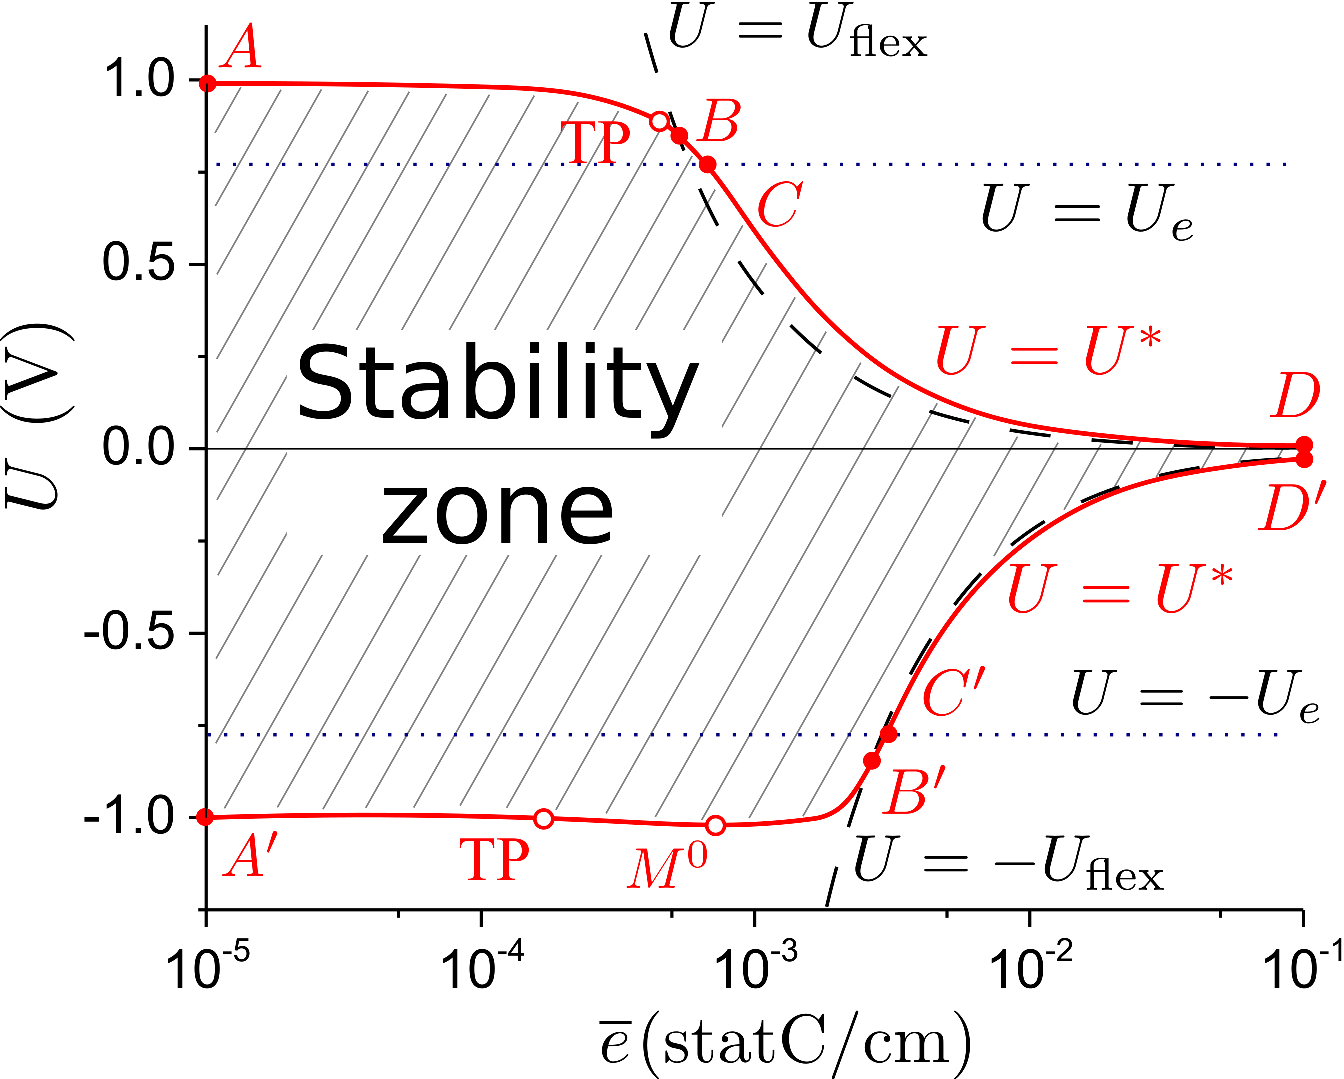
\includegraphics[width = 12cm]{Zones_and_reality_2_plots.eps}
\caption{Кривые $ABCD$ и $A'B'C'D'$, построенные при помощи формул~\eqref{eqU*analitic}, ограничивают область устойчивости планарной геликоидальной ориентационной структуры.}
\label{pic:Zones}
\end{figure}
Область устойчивости расположена между кривыми $ABCD$ и $A'B'C'D'$; они соответствуют напряжению $U = U^*(\bar{e})$.
Зоны неустойчивости планарной геликоидальной структуры расположены выше кривой $ABCD$ и ниже кривой $A'B'C'D'$.
Отметим, что зависимость $U^*$ (см. Рис.~\ref{pic-U_from_e_pos}), полученная при помощи численной минимизации функционала свободной энергии хорошо согласуется с кривой $U^*$, рассчитанной аналитически (см. Рис.~\ref{pic:Zones}).
Участки $AC$ и $A'C'$ соответствуют ситуации, когда первое из неравенств~\eqref{stab_cond_final} становится равенством, а на участках $CD$ и $C'D'$ в равенство обращается третье неравенство из~\eqref{stab_cond_final}.
Физический смысл различных участков кривых $ABCD$ и $A'B'C'D'$ можно объяснить следующим образом.
На участках $AB$ и $A'B'$ энергетически предпочтительны объёмные искажения, а искажения на границе невыгодны.
Напротив, на участках $CD$ и $C'D'$ ориентационные искажения на одной из границ выгодны, а на другой границе и в объёме -- нет.
Наконец, на участках $BC$ и $B'C'$ энергетически предпочтительны искажения в объёме и на одной из границ.
На кривых $ABCD$ и $A'B'C'D'$ знаком ``$\circ$'' отмечены трикритические точки $TP$, а также точка минимума $M^0$.
Существование точки экстремума на одной из кривых $ABCD$ или $A'B'C'D'$ -- это общее свойство систем с несимметричными энергиями сцепления $W_\theta^{(1)}\neq W_\theta^{(2)}$ (минимум на $A'B'C'D'$ при $W_\theta^{(1)}>W_\theta^{(2)}$ и максимум на $ABCD$ при $W_\theta^{(1)}<W_\theta^{(2)}$).
Координаты экстремума $M^0\big(\bar{e}^\circ,U^\circ\big)$ даются выражением
\begin{equation*}
\bar{e}^\circ=\big|{W}^{(2)}_\theta-{W}^{(1)}_\theta\big|L/4U_2,\; U^\circ =U_2\sgn\left(W_\theta^{(2)}-W_\theta^{(1)}\right).
\end{equation*}
Асмиптотика $U^*(\bar{e})$ при $\bar{e}\to\infty$ может быть записана в виде
\begin{equation}\label{A1}
U^*(\bar{e})\sim\left({K_{11}}/{4\bar{e}}\right)\left(\Delta w + 2\bar{w}\sgn(U)\sqrt{ 1+X(0)}\right),
\end{equation}
где
$X(0)=2 (t_0/\bar{w})\coth t_0 +(t_0/\bar{w})^2$, $t_0=q_0L(K_{33}/K_{11})^{1/2}.$
Из выражения~\eqref{A1} для случая $X(0)\ll1$ получаем $U^*\simeq U_\text{flex} \sgn(U)$, следовательно, линии $U^*(\bar{e})$ сближаются с пунктирными линиями на Рис.~\ref{pic:Zones}.
Таким образом, при достаточно больших значениях $\bar{e}$ флексоэлектричество облегчает переход Фредерикса, снижая пороговое напряжение.

\section{Анализ рода перехода Фредерикса при помощи разложения по низшей гармонике в двухпараметрической модели Ландау.}\label{sec:ch3/sec1}

Как показано в предыдущем разделе, планарная геликоидальная ориентационная структура при достижении напряжения $U = U^*$ теряет устойчивость из-за возможности аномального роста флуктуаций ориентации у границ ячейки, описываемых параметрами $\delta_{1,2}$.
Это даёт возможность изучить переход Фредерикса при помощи упрощённой модели, содержащей только моды с $\delta_{1,2}$.
Для этого представим зависимость $\theta(z)$ в виде
\begin{equation}\label{theta_easy}
\tilde\theta(z;\delta_1,\delta_2) = \pi/2 + \delta\psi(z;\delta_1,\delta_2),
\end{equation}
где функция $\delta\psi$ задана выражением~\eqref{psi=}.
Подставляя $\tilde\theta$ в выражение~\eqref{eq:F_for_minimization} и считая $\delta_{1,2} \ll 1$, получаем разложение свободной энергии $\FF_\mathrm{tot}$. Ограничиваясь членами четвёртого порядка малости, запишем
\begin{equation}\label{Landau_general}
\FF_\mathrm{tot}(\delta_1,\delta_2) \approx
\FF^{(0)} + \FF^{(2)}+ \FF^{(4)}=
\FF^{(0)}
+ \frac12\sum\limits_{k=0}^2A_k\delta_1^k\delta_2^{2-k}
+ \frac{1}{4!}\sum\limits_{k=0}^4 B_k\delta_1^k\delta_2^{4-k},
\end{equation}
где $\FF^{(0)}=\FF^{(0)}_f$.
Явные выражения для коэффициентов $A_k$ можно получить из выражения~\eqref{eq:Q_psi_final}:
\begin{align}
&\text{при } M > 0:\quad
	\begin{cases}\label{eq:A_k,M>0}
	A_0 = K_{11}\xi \cot{\xi L}+\EuScript{W}^{(2)}, \\
	A_1 = - 2K_{11}(\xi/\sin\xi L), \\
	A_2 = K_{11}\xi \cot{\xi L}+\EuScript{W}^{(1)},
	\end{cases} \\
&\text{при } M = 0:\quad
	\begin{cases}
	A_0 = K_{11}/L +\EuScript{W}^{(2)},\\
	A_1 = - 2(K_{11}/L),\\
	A_2 = K_{11}/L +\EuScript{W}^{(1)}.
	\end{cases}%\\
%&\text{при } M < 0:\quad
%	\begin{cases}
%	A_0 = K_{11}\xi \coth{\xi L}+\EuScript{W}^{(2)}, \\
%	A_1 = - 2K_{11}(\xi/\sinh\xi L), \\
%	A_2 = K_{11}\xi \coth{\xi L}+\EuScript{W}^{(1)}.
%	\end{cases}
\end{align}
Для случая $M < 0$ формулы для коэффициентов $A_k$ получаются из~\eqref{eq:A_k,M>0} заменой $\sin$ на $\sinh$ и $\cot$ на $\coth$.
Коэффициенты
\begin{equation}
B_k=\partial^4 \FF_\mathrm{tot}(\delta_1,\delta_2)\big/{\partial^k\delta_1 \partial^{4-k}\delta_2}\Big|_{\delta_1=\delta_2=0},
\label{eq:Bk}
\end{equation}
$k=0,\dots ,4$ \todo{Приводятся ниже/в Приложении 1/не приводятся вообще из-за громоздкости?}

Будем считать все параметры системы, кроме напряжения $U$ и усреднённого флексоэлектрического коэффициента $\bar{e}$, зафиксированными.
При достаточно низком напряжении дискриминант $A_1^2-4A_0A_2<0$, и квадратичная форма $\FF^{(2)}$ определена положительно, следовательно, планарная геликоидальная конфигурация устойчива.
С ростом напряжения при фиксированном $\bar{e}$ дискриминант $\FF^{(2)}$ обращается в ноль при $U=U^*(\bar{e})$, и соответствующее неравенство из~\eqref{stab_cond_final} становится равенством.
Наконец, при положительном дискриминанте исследуемая структура неустойчива.
%На Рис.~\ref{pic-U_from_e_pos} и Рис.~\ref{pic:Zones} приведены кривые $U=U^*(\bar{e}),на которых
Cлагаемое $\FF^{(2)}(U, \bar{e})$ обращается в ноль на кривой $U = U^*(\bar{e})$ при $\delta_2=\varkappa_* \delta_1$,
\begin{equation}
\varkappa_*(\bar{e}) = -{A_1(U^*, \bar{e} )}\big/{2A_0(U^*, \bar{e})}.
\end{equation}
Флуктуации директора в планарной геликоидальной ориентации при $U=U^*$ становятся аномально большими.
При этом род перехода (разрывный или непрерывный) определяется знаком слагаемого четвёртого порядка $\FF^{(4)}$ на прямой на плоскости параметров $(\delta_1, \delta_2)$, $\delta_2 = \varkappa_*\delta_1$.
Подставляя $U = U^*$ и $\delta_2 = \varkappa_* \delta_1$ в~\eqref{Landau_general}, получаем
\begin{equation}\label{F_4_sign}
\FF_\mathrm{tot}(\delta_1,\varkappa_*\delta_1) \approx \FF^{(0)} +\frac{1}{4!}\delta_1^4\sum\limits_{k=0}^4 B_k\varkappa_*^k\equiv\FF^{(0)} +\frac{1}{4!}\tilde{B}\delta_1^4.
\end{equation}
При $\tilde{B}=\tilde{B}(\bar{e})> 0$ переход происходит непрерывно.
Напротив, $\tilde{B} < 0$ означает, что система при $U = U^*$ уже находится в искажённом состоянии с энергией, меньшей, чем $\FF^{(0)}$. Следовательно, переход в этом случае разрывный и происходит при $U = U_c$, причём $|U_c| < |U^*|$.
Заметим, что при $\tilde{B}<0$ в модели Ландау требуется учитывать члены разложения шестого или даже более высоких порядков для того, чтобы свободная энергия была положительной при достаточно больших значениях $\delta_{1,2}$~\cite{LLStat1}.
Однако членов четвёртого порядка достаточно для анализа рода перехода.
Отметим, что схожая однопараметрическая модель Ландау для аналогичной ячейки ЖК исследовалась в работе~\cite{VAR2013} для случая $\bar{e} = 0$ с симметричными модулями сцепления с подложкой, $W_\theta^{(1)}=W_\theta^{(2)}$, и в такой системе также обнаруживается как разрывный, так и непрерывный переход.

Координаты трикритической точки $\mathrm{TP}=\left(\bar{e}^\mathrm{TP}, U^\mathrm{TP}\right)$ могут быть найдены из условий
\begin{equation}
U=U^*(\bar{e} ),\; \tilde{B}(\bar{e} )=0,
\end{equation}
причём $\tilde{B}<0$ для $\bar{e}<\bar{e}^\mathrm{TP}$ и $\tilde{B}>0$ при $\bar{e}>\bar{e}^\mathrm{TP}$.
Знак выражения $\tilde{B}(\bar{e})$ можно определить, совмещая~\eqref{theta_easy} и~\eqref{eq:F_for_minimization} и подставляя в~\eqref{eq:Bk}.
Результаты приведены на Рис.~\ref{pic:Landau}.
%Отметим, что при расчёте $\tilde{B}(\bar{e})$ используется напряжение $U^*(\bar{e})$, таким образом, в каждой точке этих зависимостей одинаковы все параметры, кроме напряжения на обкладках -- оно для каждого значения $\bar{e}$ находится отдельно.
Отметим, что на каждой кривой напряжение $U = U^*$ при соответствующем значении $\bar{e}$.
Трикритические точки определяются сменой знака $\tilde{B}$: $\bar{e}^\mathrm{TP}=5.132\times10^{-4}$~Фр/см при $U>0$ и $\bar{e}^\mathrm{TP}=1.676\times10^{-4}$~Фр/см при $U<0$.
Эти точки отмечены на Рис.~\ref{pic:Zones}, и этот результат хорошо согласуется с полученным при помощи численной минимизации свободной энергии (см. Рис.~\ref{pic-U_from_e_pos}).
\begin{figure}
	\centering
	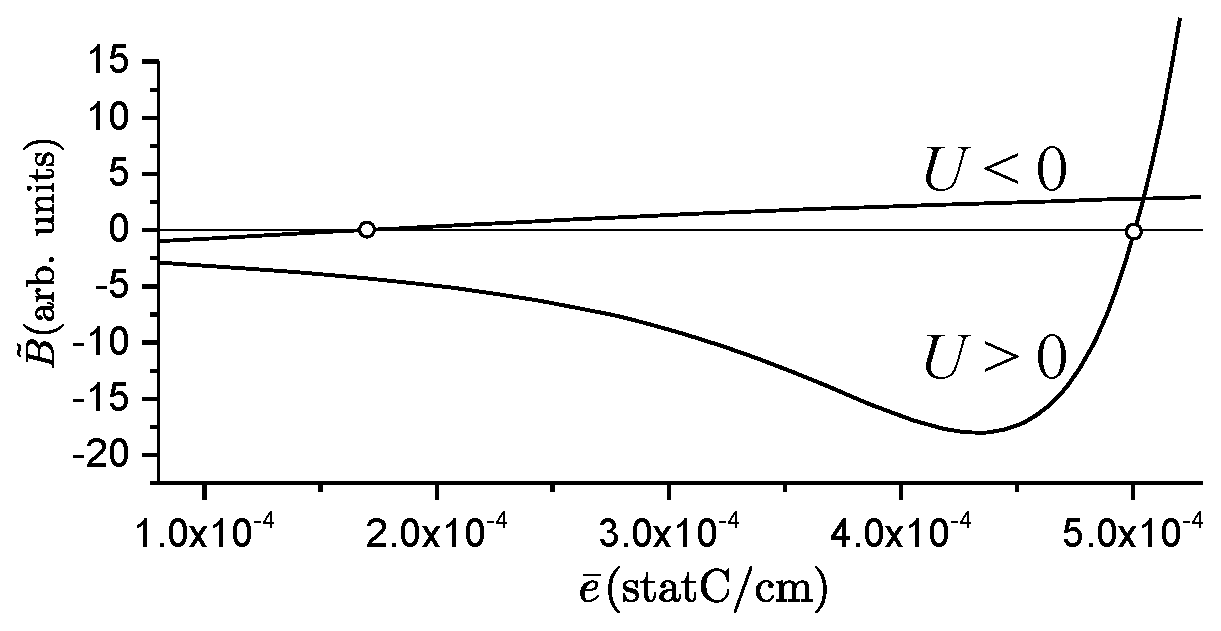
\includegraphics[angle=0,width = 10cm]{B4_pos_and_neg_voltage1.eps}
	\caption{График зависимости эффективного коэффициента $\tilde{B}$ от усреднённого флексоэлектрического коэффициента $\bar{e}$.
		Материальные параметры стандартные.
		Отметки ``$\circ$'' соответствуют трикритическим точкам.
	}
	\label{pic:Landau}
\end{figure}           % Глава 3
%\chapter{Переход Фредерикса при отрицательной анизотропии диэлектрической проницаемости.}\label{ch:ch4}

Ячейки ЖК с отрицательной анизотропией диэлектрической проницаемости отличаются тем, что, находясь во внешнем электрическом поле, молекулы ЖК стремятся выстроиться не вдоль его силовых линий, а поперёк.
Это связано со знаком $\varepsilon_a$: при $\varepsilon_a < 0$ энергия электрического поля в диэлектрике, даваемая формулой~\eqref{E_field}, становится минимальной, когда $\theta(z) = \pi/2$ на интервале $z\in [0,L]$.
Для анализа равновесной ориентационной структуры в ячейке ХЖК с отрицательной анизотропией диэлектрической проницаемости ($\varepsilon_a < 0$) вновь обратимся к методу численной минимизации функционала свободной энергии $\FF_\mathrm{tot}$.
Процедура минимизации функционала свободной энергии $\FF_\mathrm{tot}$ аналогична таковой, использованной в работе~\cite{OskirkoPRE2018}, и организована следующим образом: 

аналогично таковой в главе~\ref{ch:ch2}: представим угол $\theta(z)$ в виде
\begin{equation}\label{eq:psi+Fourier}
\theta(z) = \pi/2 +
\delta_1\frac{\sinh \xi(L-z)}{\sinh\xi L}+\delta_2\frac{\sinh\xi z}{\sinh\xi L}
+ \sum\limits_{n=1}^N c_n\sin(\pi nz/L),
\end{equation}





где  $\xi = \sqrt{\left(K_{33}q_0^2-\varepsilon_a U^2/(4\pi L^2)\right)K_{11}^{-1}}$ имеет размерность обратной длины, коэффициенты $\delta_1$, $\delta_2$  и $c_n$,  $n=1,\dots,N$ являются изменяемыми параметрами.
При этом уравнение~\eqref{eq:gran-1} позволяет сократить на 2 количество независимых параметров, а уравнение~\eqref{eq:theta'} используется для контроля точности работы минимизационного алгоритма.


\todo{Начало вставки}

Равновесную ориентационную структуру в ячейке ХЖК будем искать с помощью численной минимизации свободной энергии~\eqref{eq:F_for_minimization}, используя следующие углы лёгкого ориентирования на границах:
\begin{equation}\label{eq:initial}
\theta_0^{(1)}=\theta_0^{(2)}={\pi}/{2},\;\phi_\mathrm{tot}^{(0)}=q_0L.
\end{equation}
Эти условия соответствуют ненапряжённому ХЖК в отсутствие внешнего электрического поля.
Сведём задачу поиска минимума функционала $\FF_\mathrm{tot}[\theta(z)]$ к задаче поиска минимума функции нескольких переменных, аппроксимировав искомую зависимость $\theta(z)$ пробной функцией
\begin{equation}\label{eq:psi+Fourier}
\theta(z) =
\pi/2 + {\delta\psi}(z,\delta_1,\delta_2) + \sum\limits_{n=1}^N c_n\sin(\pi nz/L).
\end{equation}
Здесь слагаемое $\pi/2$ соответствует неискажённому состоянию.
Функция $\delta\psi(z,\delta_1,\delta_2)$, задаваемая выражением~\eqref{psi=}, содержит $\delta_1$ и $\delta_2$ -- отклонения от углов лёгкого ориентирования на границах: $\theta(0) = \pi/2 + \delta_1$, $\theta(L) = \pi/2 + \delta_2$.
Наконец, ряд Фурье описывает объёмные искажения ориентационной структуры, не затрагивающие границы.
Используя граничные условия~\eqref{eq:gran-1}, можно выразить коэффициенты $c_N$ и $c_{N-1}$ через все остальные -- $\delta_{1,2}$ и $\{c_n\}_{n=1}^{N-2}$.
Таким образом, углы $\delta_1$, $\delta_2$, а также коэффициенты $c_n$, $n=1,\dots,N-2$ являются регулируемыми параметрами.

Ограничимся в~\eqref{eq:psi+Fourier} $N = 20$ членами ряда Фурье.
Учёт более, чем 20 слагаемых приводит к относительному изменению профиля $\theta$ менее чем на $0.5\%$ для любого $z$ на всём интервале $[0,\, L]$.
В многомерной численной минимизации существует проблема попадания в максимумы или в седловые точки.
Для того, чтобы определить, действительно ли минимизация свободной энергии привела к минимуму, используем случайные небольшие сдвиги параметров  $\delta_{1,2}$, $\{c_n\}$ относительно полученных значений.
Если минимизационный алгоритм приводит к другому ответу, это означает, что предыдущий результат был ошибочным -- максимумом или седловой точкой.
При этом в случае, если достигнут, по крайней мере, локальный минимум, то при любом достаточно небольшом сдвиге минимизация будет всегда возвращать нас обратно.

Будем изменять напряжение $U$, зафиксировав все остальные параметры ячейки ЖК.
\begin{figure}
	\centering
	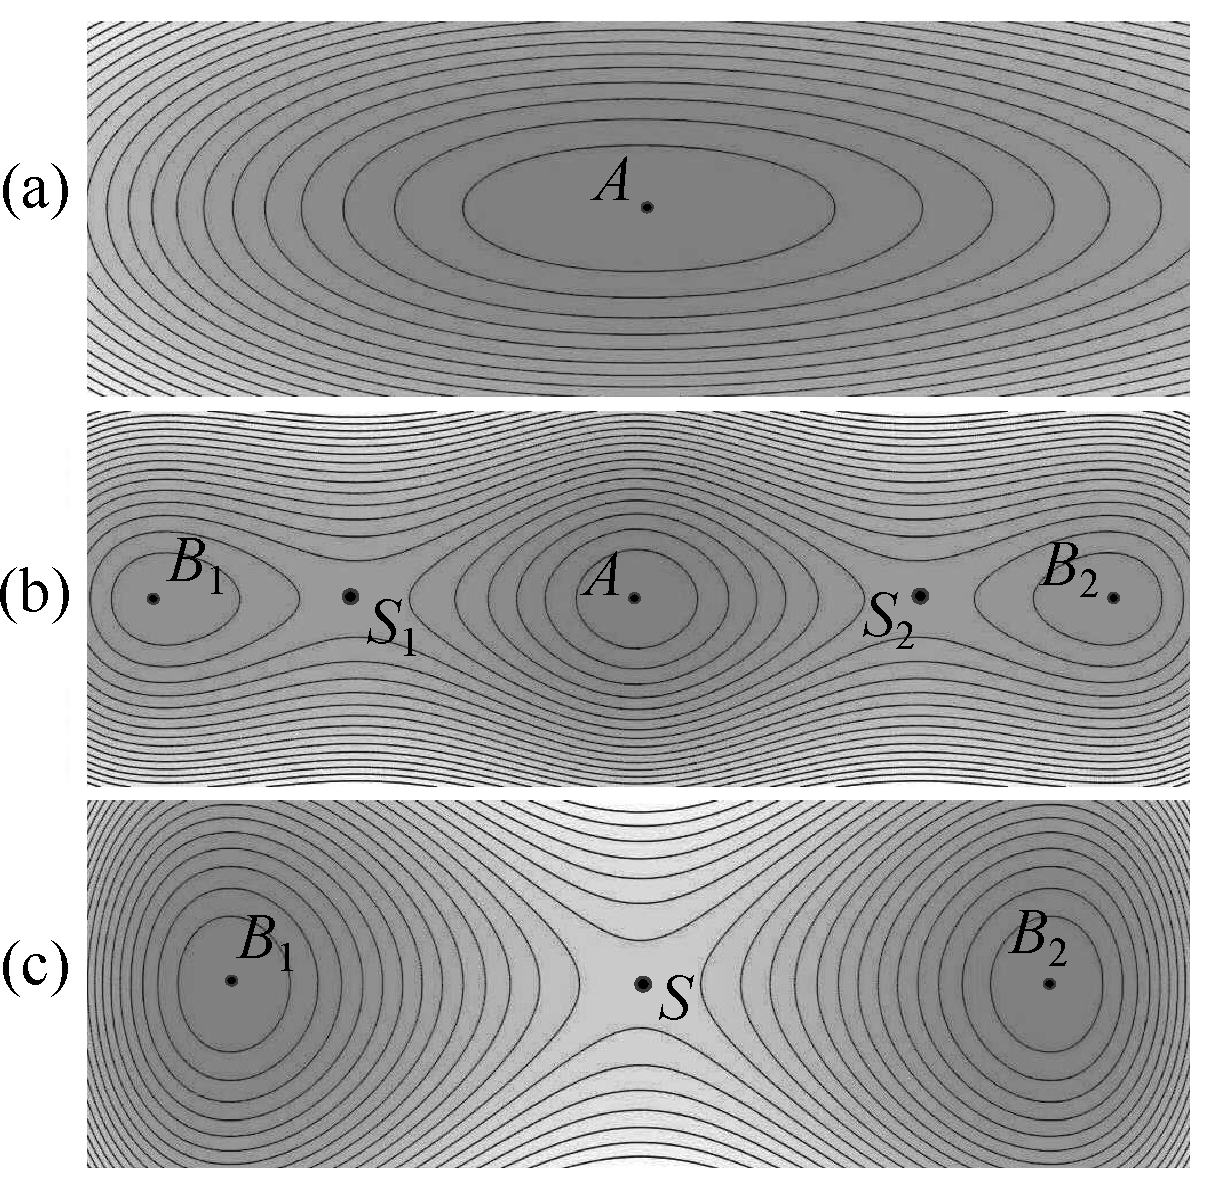
\includegraphics[width = 15cm]{Geo_final.eps}
	\caption{Схематичное двумерное изображение случаев, возникающих при численной минимизации свободной энергии}
	\label{pic_Geo_final}
\end{figure}
При этом будет наблюдаться один из трёх случаев, проиллюстрированных на Рис.~\ref{pic_Geo_final}:
\begin{enumerate}
	\item[(a)]
	Существует единственный минимум (точка А на рис.~\ref{pic_Geo_final}a), соответствующий планарной геликоидальной структуре, при этом $\delta_{1,2}=0$, $c_n = 0$, то есть $\theta(z)=\pi/2$, а $\phi(z) = q_0z$.
	\item[(b)]
	Случай трёх минимумов.
	Один из них (точка А на Рис.~\ref{pic_Geo_final}b) по-прежнему соответствует планарной геликоидальной структуре.
	Два других (точки $B_1$ и $B_2$) соответствуют искажённым структурам, то есть таким, для которых некоторые из параметров $\delta_{1,2}$, $c_n$ ненулевые.
	При этом параметры $(\delta_{1},\delta_{2},c_n)$, соответствующие точкам $B_1$ и $B_2$, отличаюся только знаком, следовательно, этим двум точкам соответствуют одинаковые распределения директора ввиду симметрии относительно замены ${\bf n} \leftrightarrow -{\bf n}$.
	\item[(c)]
	Имеются ровно два минимума.
	В этом случае существуют два минимума $B_1$ и $B_2$, соответствующие одной и той же искажённой ориентационной структуре.
	Планарная геликоидальная структура здесь не существует, так как является седловой точкой ($S$ на Рис.~\ref{pic_Geo_final}c).
\end{enumerate}
Здесь и далее мы будем называть ''устойчивыми'' равновесные состояния, соответствующие локальным минимумам свободной энергии, а ''метастабильными'' -- устойчивые состояния с энергией, большей, чем у другого устойчивого состояния.

\subsubsection{"Фазовая" \todo{(Структурная?)} диаграмма}

Случай (a) на Рис.~\ref{pic_Geo_final} возникает для напряжений $|U|$ ниже порогового значения $U^{**}$, а при достижении этого значения могут наблюдаться две различные ситуации.
Они соответствуют разрывному (I) и непрерывному (II) переходу Фредерикса:
\begin{itemize}
	\item[I.]
	В этом случае существует ещё одно пороговое значение $U^{*} > U^{**}$, при этом для $|U|\in (U^{**},\, U^{*})$ у функционала свободной энергииесть сразу три локальных минимума, из которых один соответствует начальной планарной геликоидальной структуре	, а два других -- искажённой ориентационной структуре, как показано на Рис.\ref{pic_Geo_final}b.
	Здесь $U^{**}$ -- наименьшее напряжение, при котором искажённая ориентационная структура ещё может существовать в качестве метастабильной, а, в свою очередь, $U^{*}$ -- максимальное напряжение, при котором планарная геликоидальная структура ещё может существовать как метастабильная.
	Таким образом, при любом $U$ из интервала $(U^{**},\,U^*)$ только одна из структур будет стабильной (с меньшей энергией), в то время как другая будет метастабильной.
	С ростом напряжения $|U|$ свободная энергия искажённой структуры уменьшается, и при $|U| = U_c$ становится равной энергии неискажённого состояния, и происходит разрывный переход Фредерикса.
	То есть, при $|U| < U_c$ более энергетически выгодным является неискажённое состояние, а при $|U| > U_c$ -- искажённое.
	Наконец, при $|U|>U^*$ реализуется случай (c).
	\item[II.]
	В данном сценарии существует только одно пороговое напряжение, $|U| = U_c$. Этот сценарий соответствует (I) для $U^{*} = U_c = U^{**}$, при этом происходит непрерывный переход Фредерикса. 
	Здесь при $|U| < U_c$ возникает случай (a), а при  $|U|>U_c$ -- случай (c), показанные на Рис.~\ref{pic_Geo_final}c.
\end{itemize}
Интервалы стабильности и метастабильности схематично изображены на Рис.~\ref{pic-U*U**Uc_otline}.
\begin{figure}%[thb]
	\centering
	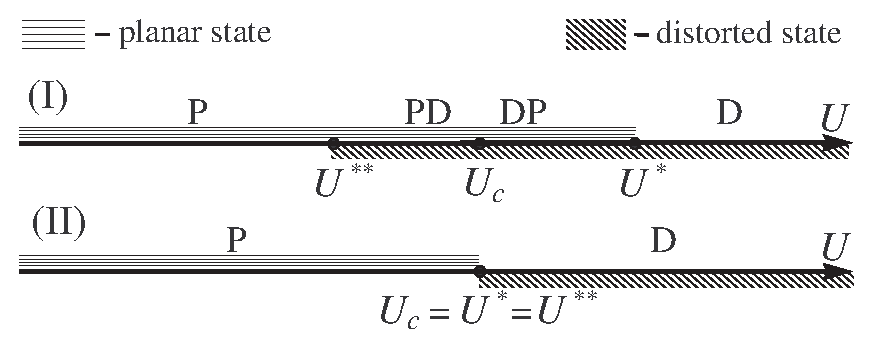
\includegraphics[width=12cm]{UU1d3a.eps}
	\caption{Иллюстрация разрывного (I) и непрерывного (II) переходов Фредерикса для $U > 0$.
		(I): Области устойчивости искажённой (D) структуры, $U>U^{**}$, и неискажённой (P) структуры, $U<U^{*}$.
		На интервале, обозначенном PD, $U^{**}<U<U_c$, искажённая структура метастабильна, а на интервале DP, $U_c < U < U^{*}$, метастабильна планарная геликоидальная структура.
		(II):  Области устойчивости для искажённой, $U > U_c$, и неискажённой структуры, $U < U_c$.}
	\label{pic-U*U**Uc_otline}
\end{figure}

Для того, чтобы изучить, как влияет флексоэлектрическая поляризация на переход Фредерикса, были рассчитаны пороговые напряжения $U^{**}$, $U_c$, $U^{*}$ для различных значений усреднённого флексоэлектрического коэффициента $\bar{e}$.
Отметим, что учёт флексоэлектричества привёл к тому, что значения напряжений $U^{**}$, $U^*$ и $U_c$ стали различными для  $U>0$ и $U<0$, если константы сцепления с подложкой различны, $W_\theta^{(1)}\not=W_\theta^{(2)}$.
Значения материальных констант были взяты такими же, как и в~~\cite{VAR2013}: $K_{11}=0.42\times 10^{-6}$~дин, $K_{22}=0.23\times 10^{-6}$~дин, $K_{33}=0.53\times 10^{-6}$~дин,  $q_0=500$~$\text{cm}^{-1}$, $L=60$~$\mu\text{m}$, $W_\theta^{(1)}=2.5\times 10^{-3}$~эрг/см$^2$, $W_\theta^{(2)}=0.5\times 10^{-3}$~эрг/см$^2$,  $W_\phi^{(1)}=2.5\times 10^{-4}$~эрг/см$^2$, $W_\phi^{(2)}=1.0\times 10^{-4}$~эрг/см$^2$, $\varepsilon_\bot=7.2$, $\varepsilon_\|=16.2$.
\todo{В дальнейшем будем называть этот набор параметров стандартным.}
Выбранные значения параметров $q_0$ и $L$ соответствуют супертвист-ячейке ЖК с полной закруткой $q_0L = 3>\pi/2$.
Кроме того, значения констант сцепления с подложкой выбраны сильно различающимися, чтобы продемонстрировать влияние такой асимметрии границ.
На Рис.~\ref{pic-U_from_e_pos} представлена рассчитанная "фазовая диаграмма" в координатах ($\bar{e}$, $U$) для обоих направлений электрического поля.
\begin{figure}%[bht]
	\centering
	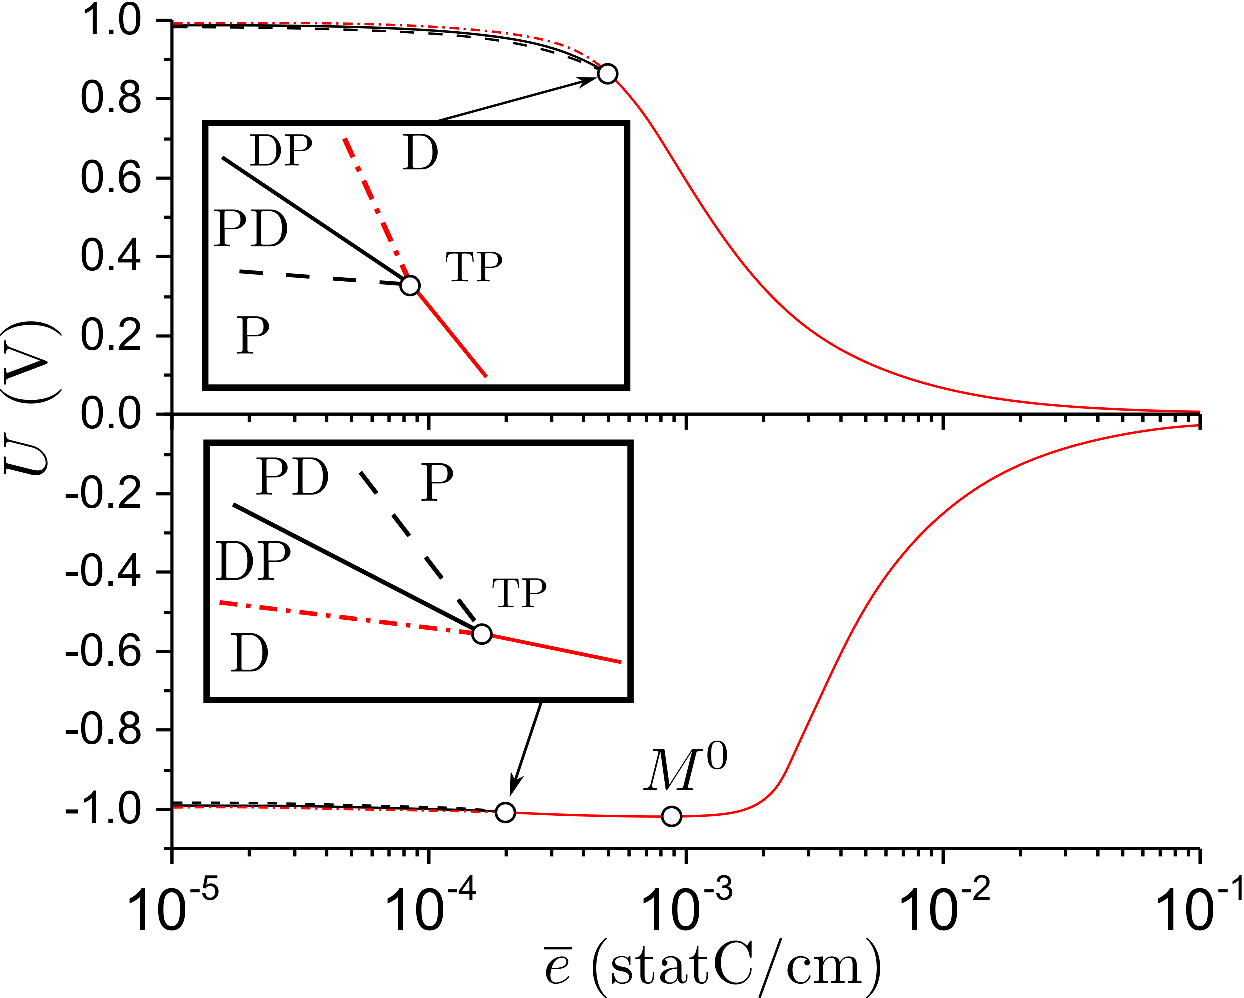
\includegraphics[width=15cm]{Graph7colorB.eps}
	\caption{Фазовая диаграмма.
		Напряжения $U^*$, $U_c$ и $U^{**}$ как функции усреднённого флексоэлектрического коэффициента $\bar{e}$: пунктирная линия -- $U^{**}$, сплошная линия -- $U_c$, штрихпунктирная линия -- $U^{*}$.
		Области стабильности и метастабильности обозначены на вставках.
		Трикритические точки обозначены как TP, другие обозначения совпадают с таковыми на Рис.~\ref{pic-U*U**Uc_otline}.
		Правее трикритической точки TP линии $U^*$, $U_c$ и $U^{**}$ совпадают.}
	\label{pic-U_from_e_pos}
\end{figure}






\todo{Конец вставки}

При помощи минимизации свободной энергии были найдены равновесные ориентационные структуры в ячейке ХЖК при различных значениях усреднённого флексоэлектрического коэффициента $\bar{e}$ и приложенного напряжения $U$, а также следующих значениях материальных констант: $K_{11}=0.42\times 10^{-6}$~дин, $K_{22}=0.23\times 10^{-6}$~дин, $K_{33}=0.53\times 10^{-6}$~дин,  $q_0=500$~$\text{cm}^{-1}$, $L=60$~$\mu\text{m}$, $W_\theta^{(1)}=2.5\times 10^{-3}$~эрг/см$^2$, $W_\theta^{(2)}=0.5\times 10^{-3}$~эрг/см$^2$,  $W_\phi^{(1)}=2.5\times 10^{-4}$~эрг/см$^2$, $W_\phi^{(2)}=1.0\times 10^{-4}$~эрг/см$^2$, $\varepsilon_\bot=16.2$, $\varepsilon_\|=7.2$.
Заметим, что от стандартного набора параметров этот набор отличается только значениями диэлектрической проницаемости $\varepsilon_\bot$ и $\varepsilon_\|$.

Полученные результаты для $\varepsilon_a < 0$ для сравнения приводятся вместе с аналогичными результатами для $\varepsilon_a > 0$. На Рис.~\ref{fig1} на плоскости $(\bar{e},U)$ приведены рассчитанные области устойчивости планарной геликоидальной ориентационной структуры.
\begin{figure}
	\centering
	\includegraphics[width=0.49\textwidth]{1aa.eps}%{PhD_negative_ea.png}\hspace{2pc}%
	\hfill
	\includegraphics[width=0.49\textwidth]{1bb.eps}%{PhD_negative_ea.png}\hspace{2pc}%
	\caption{Фазовые диаграммы для случаев $\varepsilon_a < 0$ и $\varepsilon_a > 0$. Сплошной и пунктирной линией обозначена граница между различными "фазами" при разрывном и непрерывном переходе соответственно.
		Точечной линией обозначена асимптота межфазовой границы при $\varepsilon_a < 0$, а знаком ``$\circ$'' -- трикритическая точка.}\label{fig1}
\end{figure}
Данный результат можно получить и аналитически аналогично тому, как это было проделано в Главе~\ref{ch:ch3}.
Для этого следует изучить знак второй вариации функционала свободной энергии на планарной геликоидальной структуре $\delta^2 \FF_\mathrm{tot}(\theta_0,\phi_0)$.
При этом вклад, связанный с вариацией $\phi$, всегда неотрицателен, а вклад, связанный с вариацией $\theta$, даётся формулой~\eqref{d2F_theta}.
Важным отличием от случая $\varepsilon_a > 0$ является то, что $M > 0$ при любых значениях напряжения $U$.
Это приводит к тому, что после выполнения разбиения $\delta^2\FF_\theta = (Q_\mu + Q_\psi)S_\bot/2$ первое слагаемое оказывается всегда неотрицательным.
Приведём явный вид $Q_\psi$ для случая $\varepsilon_a < 0$:
\begin{equation}
Q_\psi = \sum\limits_{\alpha=1,2}\left(K_{11}\xi \coth{\xi L}+\EuScript{W}^{(\alpha)}\right) \delta_\alpha^2\\
- 2K_{11} (\xi/\sinh\xi L)\delta_1\delta_2,
\end{equation}
$\xi$ задаётся формулой~\eqref{xi=}.
Требование положительности $Q_\psi$ приводит к третьему неравенству в~\eqref{eq:ineq_M>0_final_c}:
\begin{equation}
w^{(1)} w^{(2)} + 2\bar{w} t \coth{t} + t^2 > 0,
\end{equation}
где $t = \xi L$.
Это нервенство квадратично относительно $\bar{e}$, и его решение даётся неравенствами~\eqref{eq:interval_1} и~\eqref{eq:interval_2} при $U_1\to\infty$.
Приведём явный вид решения:
\begin{align}
&0\leq \bar{e}\leq+\infty,\!  &&\text{если }U = 0,\\
&0\leq \bar{e} < e_+^*,\!  &&\text{если }0<|U|<\infty,
\end{align}
где
\begin{equation}\label{eq:e(U)_ea<0}
e_+^*(U)=\left(K_{11}/4U\right)\left(\Delta{w}
+ 2\bar{w}\sgn{U}\sqrt{ 1+X(U) }\right) ,
\end{equation}
\begin{equation}\label{eq:X(U)_ea<0}
X(U)=\frac{2}{\bar{w}}\left( t\coth t +{t^2}/2\bar{w}\right).
\end{equation}
Кривая $e^*_+(U)$, построенная по выражению~\eqref{eq:e(U)_ea<0}, совпадает с расчётной кривой $U^*(\bar{e})$.
Кроме того, можно рассчитать положение вертикальной асимптоты $\bar{e}'$:
\begin{equation}
\bar{e}' = \lim_{U\to \infty} \bar{e}^*_+(U) = \sqrt{\frac{-\ve_a K_{11}}{16\pi}}
\end{equation}
Подставляя указанные выше значения параметров, получаем $\bar{e}' =2.74\times 10^{-4} $~Фр/см, что также хорошо согласуется с численными расчётами.

Отметим важные свойства диаграммы в случае $\varepsilon_a < 0$.
С одной стороны, переход Фредерикса оказывается невозможен при небольших значениях $\bar{e}$.
Этот результат, в частности, согласуется с эмпирическим представлением о том, как должны выстраиваться молекулы с отрицательной анизотропией диэлектрической проницаемости во внешнем электрическом поле в отсутствие флексоэлектрической поляризации.
С другой стороны, существует некоторое значение $\bar{e}'$ такое, что при $\bar{e} > \bar{e}'$ переход возможен, причём напряжение, необходимое для этого, убывает убывает с ростом $\bar{e}$.
Таким образом, кривая зависимости $U = U^*(\bar{e})$ имеет две асимптоты: горизонтальную $U = 0$ и вертикальную $\bar{e} = \bar{e}' =2.74\times 10^{-4} $~Фр/см.
Также отметим, что в случае $\ve_a < 0$ возможен только непрерывный переход Фредерикса.
\todo{Этот вывод можно сделать как по результатам численной минимизации свободной энергии, так и при помощи способа оценки рода перехода Фредерикса, описанном в предыдущей главе: коэффициент $\tilde{B}$ оказывается положительным.}

\todo{После этой надписи идёт черновик-черновик}

%На Рис.~\ref{fig1} можно увидеть довольно неожиданный результат для $\varepsilon_a<0$.
%Оказалось, что существует такое значение $\bar{e}$ (вертикальная асимптота), выше которой может существовать искажённая структура.
%Ниже этого предела искажённая фаза не может существовать ни при каком значении $U$.
На Рис.~\ref{fig2} приведены профили полярного угла $\theta(z)$, рассчитанные при фиксированном напряжении $U = 1.2$~В и различных значениях $\bar{e}$.
\begin{figure}
	\centering
	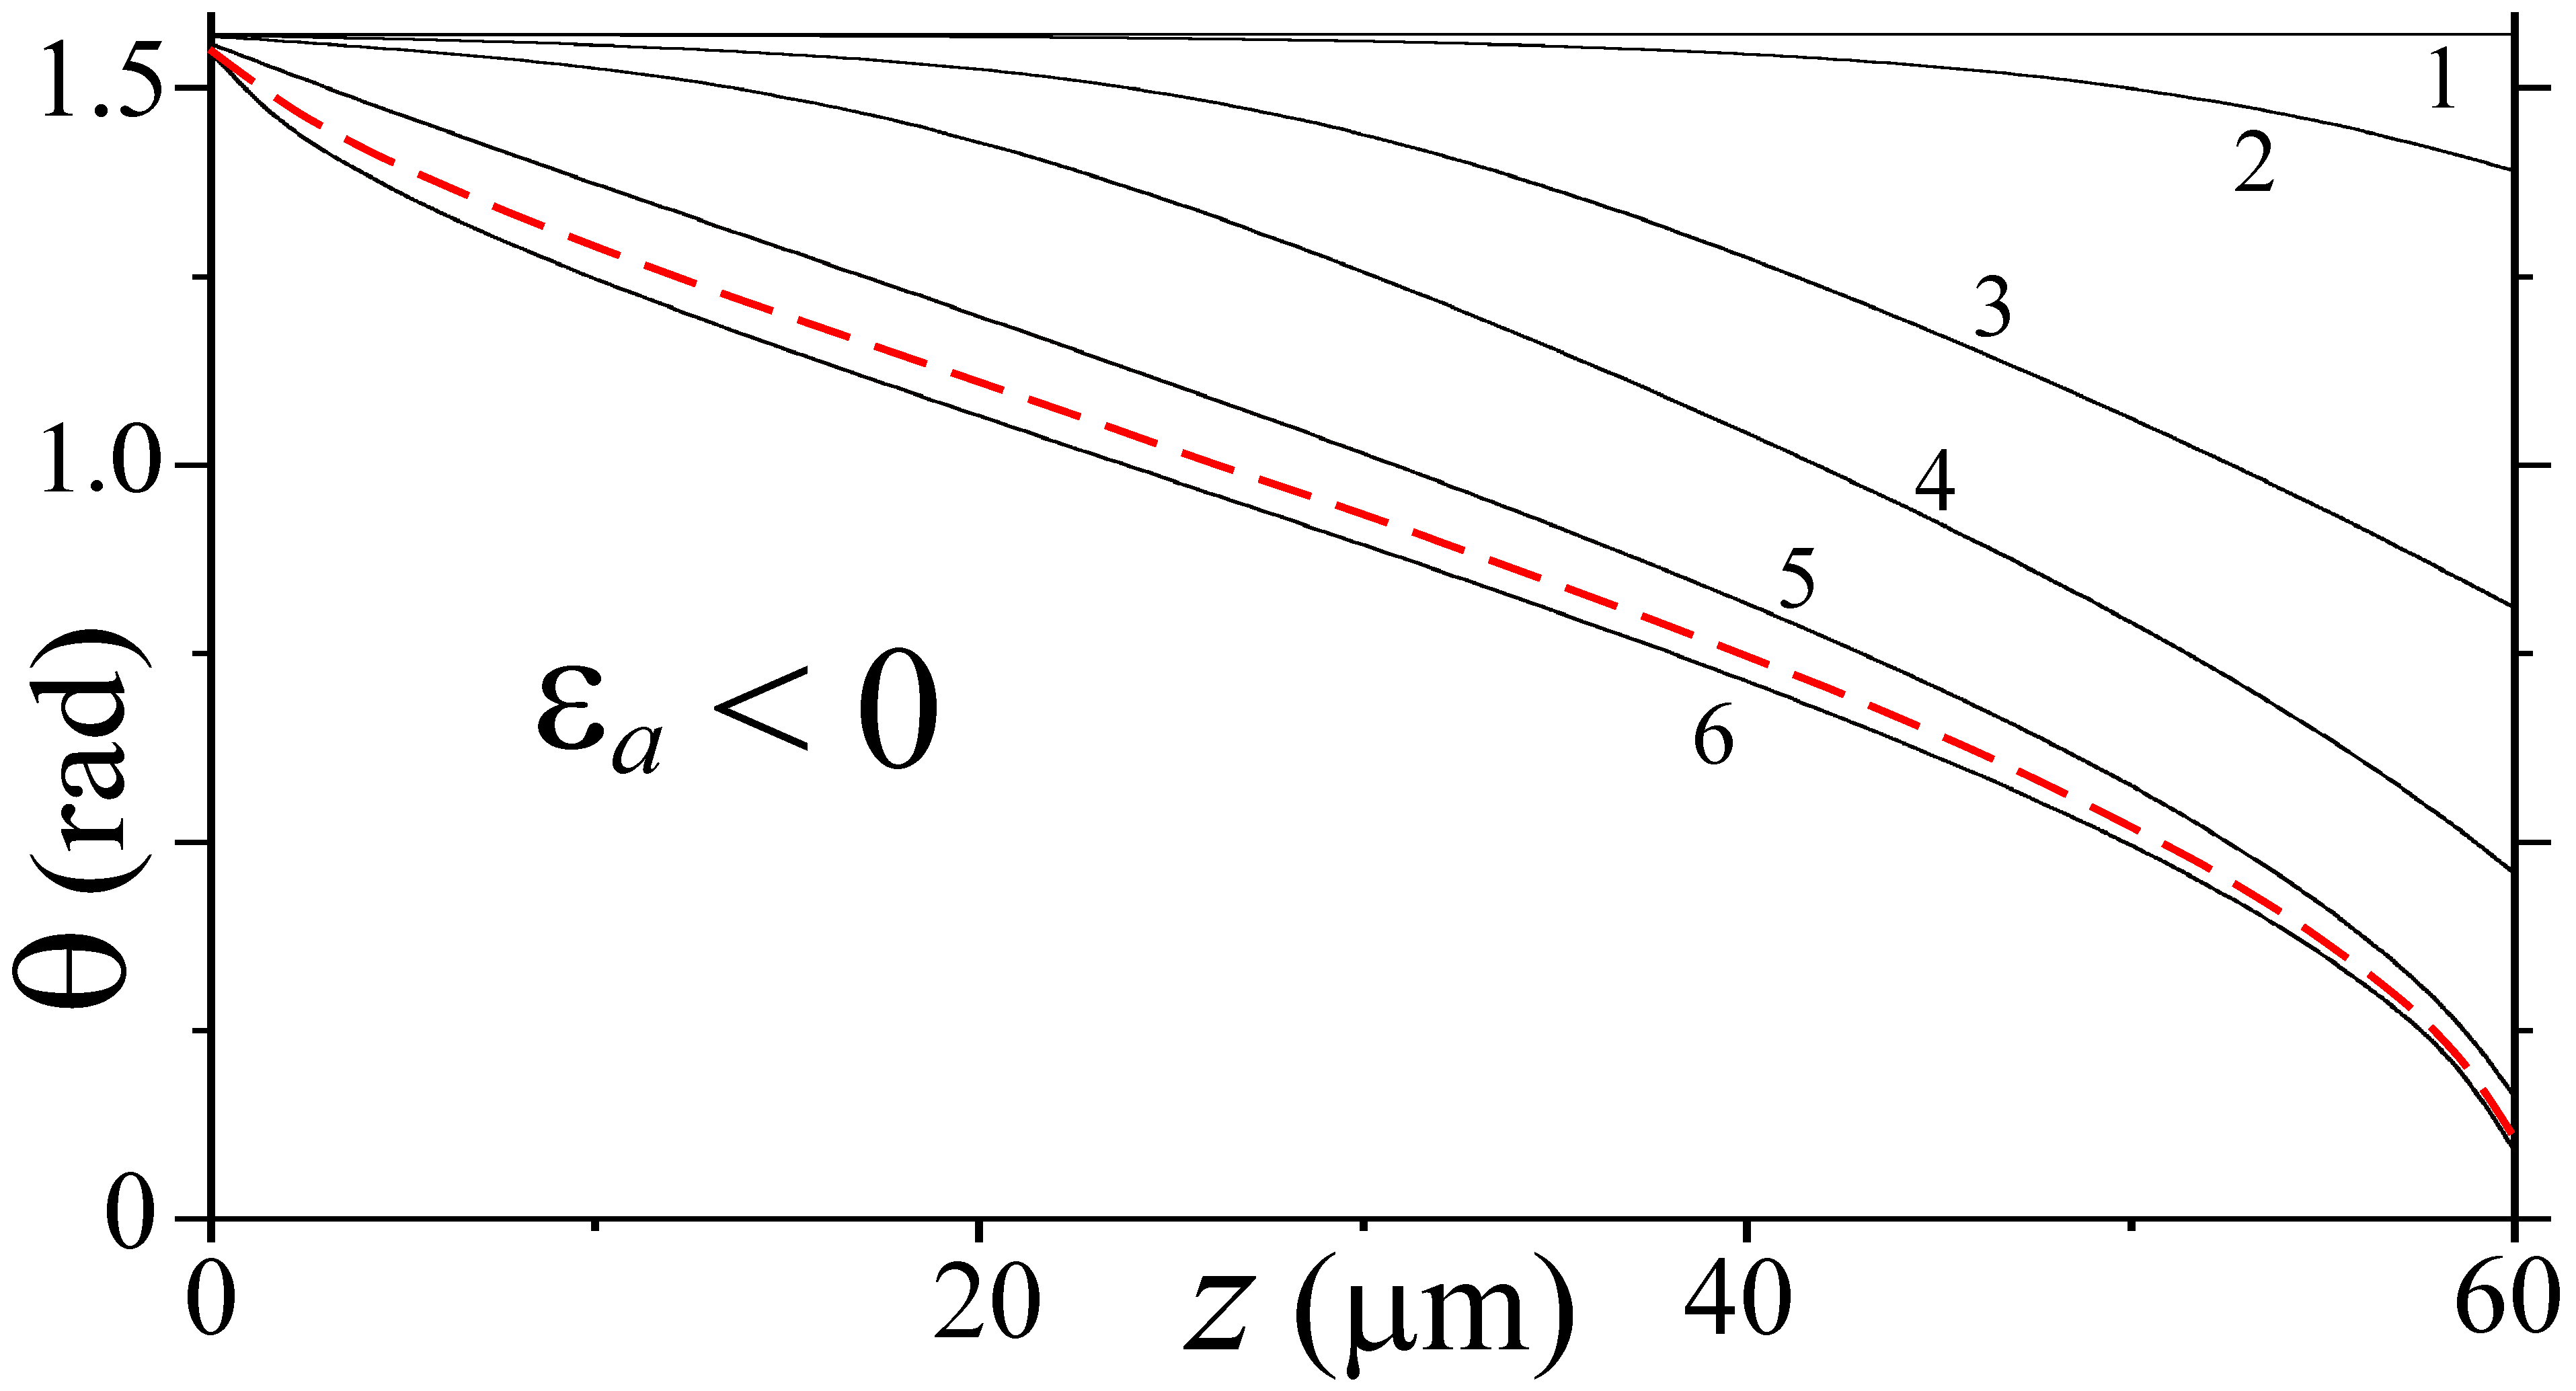
\includegraphics[width=0.49\textwidth]{Fig4_parody1a.eps}
	\hfill
	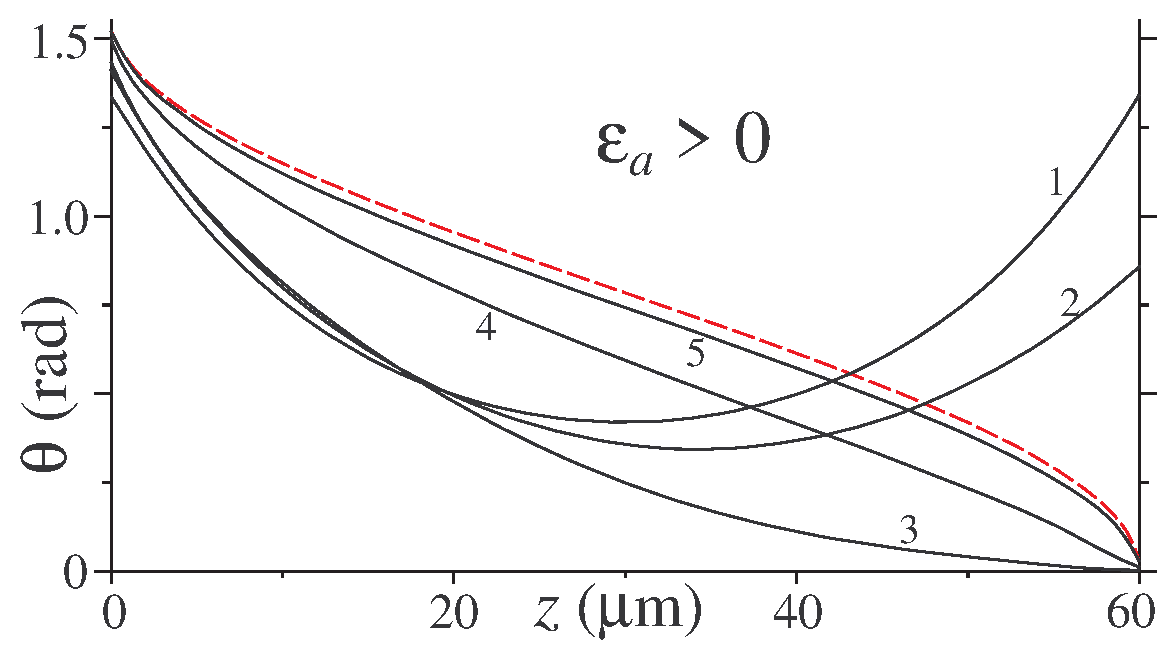
\includegraphics[width=0.49\textwidth]{symm_all_6curvesNoReflect1b.eps}
	\caption{Графики зависимости $\theta(z)$ при $U=1.2$~В.
		Значения $\bar{e}$ в единицах $\mathrm{statC/cm}$ для случая $\varepsilon_a < 0$: 1 -- $\bar{e}=10^{-3}$, 2 -- $\bar{e}=1.5\times 10^{-3}$, 3 -- $\bar{e}=1.8\times 10^{-3}$, 4 -- $\bar{e}=2\times 10^{-3}$, 5 -- $\bar{e}=3\times 10^{-3}$, 6 -- $\bar{e}=10^{-2}$; значения $\bar{e}$ при $\varepsilon_a > 0$: 1 -- $\bar{e}=0$, 2 -- $\bar{e}=10^{-4}$, 3 -- $\bar{e}=10^{-3}$, 4 -- $\bar{e}=3\times 10^{-3}$, 5 -- $\bar{e}=10^{-2}$ в единицах $\text{Фр}/\text{см}$.
		Красные пунктирные линии соответствуют зависимости $\cos^2\theta(z)\simeq {z/L}$.}\label{fig2}
\end{figure}
В случае, когда $\bar{e}$ достаточно мал, равновесные ориентационные структуры значительно отличаются для $\varepsilon_a > 0$ и $\varepsilon_a < 0$.
Однако с ростом $\bar{e}$ ориентационные структуры становятся очень схожи.
Это интересное свойство может быть объяснено следующим образом.
Выражение для свободной энергии~\eqref{eq:free-energy} при больших значениях $\bar{e}$ и/или $U$ (когда вкладами, содержащими $K_{ii}$ и $W^{(\alpha)}_{\theta,\varphi}$, можно пренебречь), сводится к следующему:
\begin{equation}\label{eq_F_f_final123}
\FF\simeq-\frac{S_{\!\bot}}{8\pi}U^2 J +S_{\!\bot} \bar{e}U JJ_1 + 2\pi S_{\!\bot} \bar{e}^2\int_{0}^{L}\frac{(\sin 2\theta \,\theta'-JJ_1)^2}{{\EE}(\theta)}dz.
\end{equation}
Рассмотрим ситуацию, когда вклады, содержащие $\bar{e}$, значительно превосходят первый вклад в~\eqref{eq_F_f_final123}.
Чтобы выяснить критерий наступления этого случая, оценим по модулю отношение второго слагаемого в~\eqref{eq_F_f_final123} к первому:
\begin{equation}\label{ch4:eq_e/U>>1}
\frac{8\pi\bar{e}UJJ_1}{U^2 J}\sim \frac{\bar{e}}{\ve_a U} \gg 1
\end{equation}
Последнее неравенство и является критерием.
Кроме того, в ситуации, когда $\sin 2\theta \,\theta'-JJ_1\neq 0$, это же неравенство означает превосходство последнего слагаемого в~\eqref{eq_F_f_final123} над остальными.
Определим, какой профиль $\theta(z)$ даёт доставляет минимум функционалу~\eqref{eq_F_f_final123}, когда выполнено условие~\eqref{ch4:eq_e/U>>1}.
Можно заметить, что интеграл в слагаемом, содержащем $\bar{e}^2$, неотрицателен, а значит, на равновесной ориентационной конфигурации $\theta(z)$ должен быть близок к нулю.
Это достигается, когда выполнено следующее равенство:
\begin{equation}
\sin 2\theta \,\theta'-JJ_1 = 0.
\end{equation}
Общим решением этого дифференциального уравнения является функция $\theta(z)$, для которой
\begin{equation}\label{ch4:eq_cos2=az+b}
\cos^2\theta(z) = az+b
\end{equation}
с произвольными константами $a$ и $b$.
Так как третье слагаемое в~\eqref{eq_F_f_final123} близко к нулю, минимум свободной энергии определяется вторым слагаемым.
Подставляя~\eqref{ch4:eq_cos2=az+b} в~\eqref{eq_F_f_final123} и опуская первое слагаемое, получаем
\begin{equation}
\FF \simeq -S_\bot \bar{e} U a.
\end{equation}
Таким образом, минимуму $\FF$ соответствует максимальное положительное значение $a$.
Для его определения учтём ограничения на $a$ и $b$, следующие из определения~\eqref{ch4:eq_cos2=az+b}:
\begin{equation}\label{ch4:eq_rectangle01}
0 \leq az + b \leq 1
\qquad \forall z\in [0,\ L]
\end{equation}
Таким образом, отрезок прямой $az+b$ на $z\in[0,\ L]$ должен целиком находиться в области, изображённой на Рис.~\ref{ch4:pic_rectangle01}, то есть его левый конец должен лежать на левой границе приведённой области, а правый -- на правой.
\begin{figure}\label{ch4:pic_rectangle01}
	\centering
	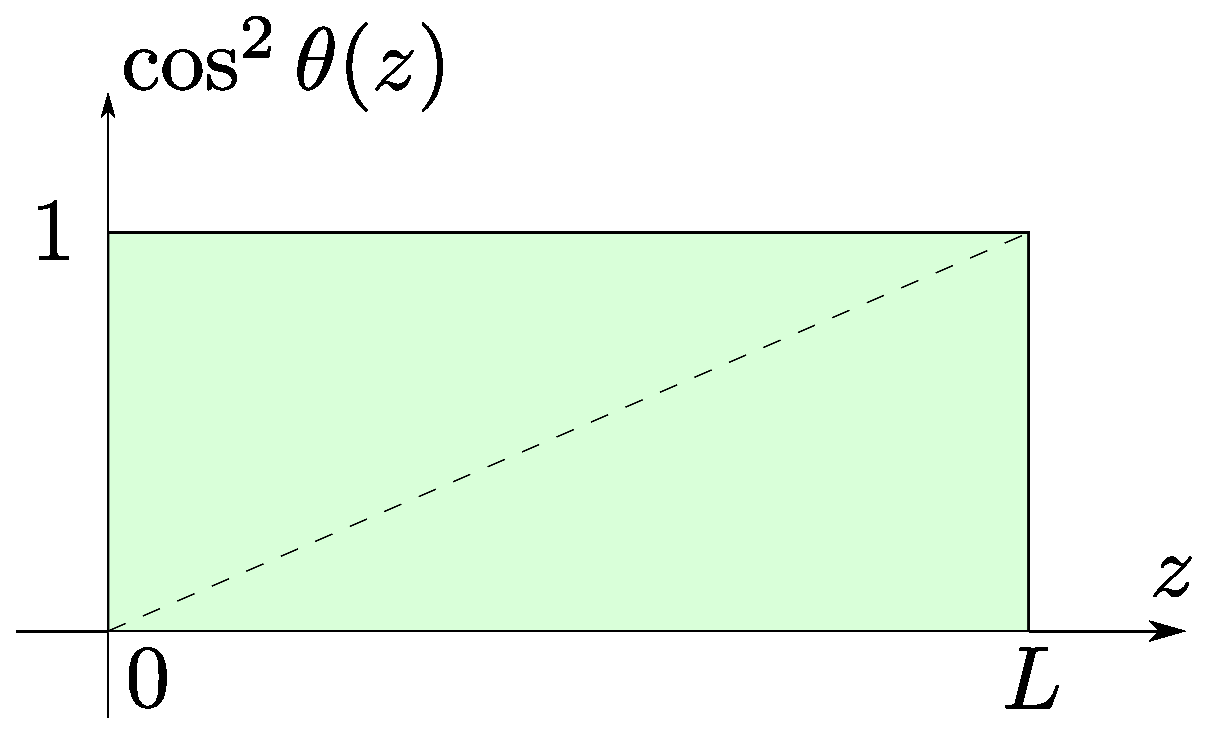
\includegraphics[width=8cm]{rectangle01}
	\caption{Область, задаваемая неравенствами~\eqref{ch4:eq_rectangle01} и отрезок прямой с наибольшим возможным угловым коэффициентом.}
\end{figure}
Нетрудно заметить, что наибольшее положительно значение $a$ соответствует прямой, отмеченной на Рис.~\ref{ch4:pic_rectangle01}  пунктиром, и равняется $1/L$, $b = 0$.
Таким образом, минимум функционала $\FF$ как при $\varepsilon_a<0$, так и при $\varepsilon_a>0$ даётся зависимостью $\cos^2\theta(z)\simeq {z/L}$.
Отметим, что при достаточно больших $\bar{e}$ равновесной является гибридно-ориентированная структура.
В такой структуре рядом с одной из границ молекулы в среднем выстраиваются параллельно ограничивающей плоскости, а рядом с другой -- перпендикулярно. ~\todo{можно вставить красивый рисунок-иллюстрацию.}
Такой переход между планарной геликоидальной и гибридной структурами может быть использован для создания переключателей, в основе работы которых лежит флексоэлектричество.

Кроме того, в ячейке ХЖК с достаточно большим $\bar{e}$ был обнаружен ориентационный переход нового типа.
Такой переход продемонстрирован на Рис.~\ref{fig4_3}, где представлены профили $\theta(z)$ при фиксированном $\bar{e}$ и различных значениях напряжения $U$.
С ростом приложенного напряжения от нулевого значения сначала происходит непрерывный переход Фредерикса.
При дальнейшем увеличении напряжения происходит ещё один переход.
Этот переход является разрывным, так как происходит между двумя значительно различающимися ориентационными структурами.
Это иллюстрируют графики 2 и 3 на Рис.~\ref{fig4_3}: разница в приложенном напряжении составляет $0.01$~В, при этом полученные профили существенно различны.
\begin{figure}
	\centering
	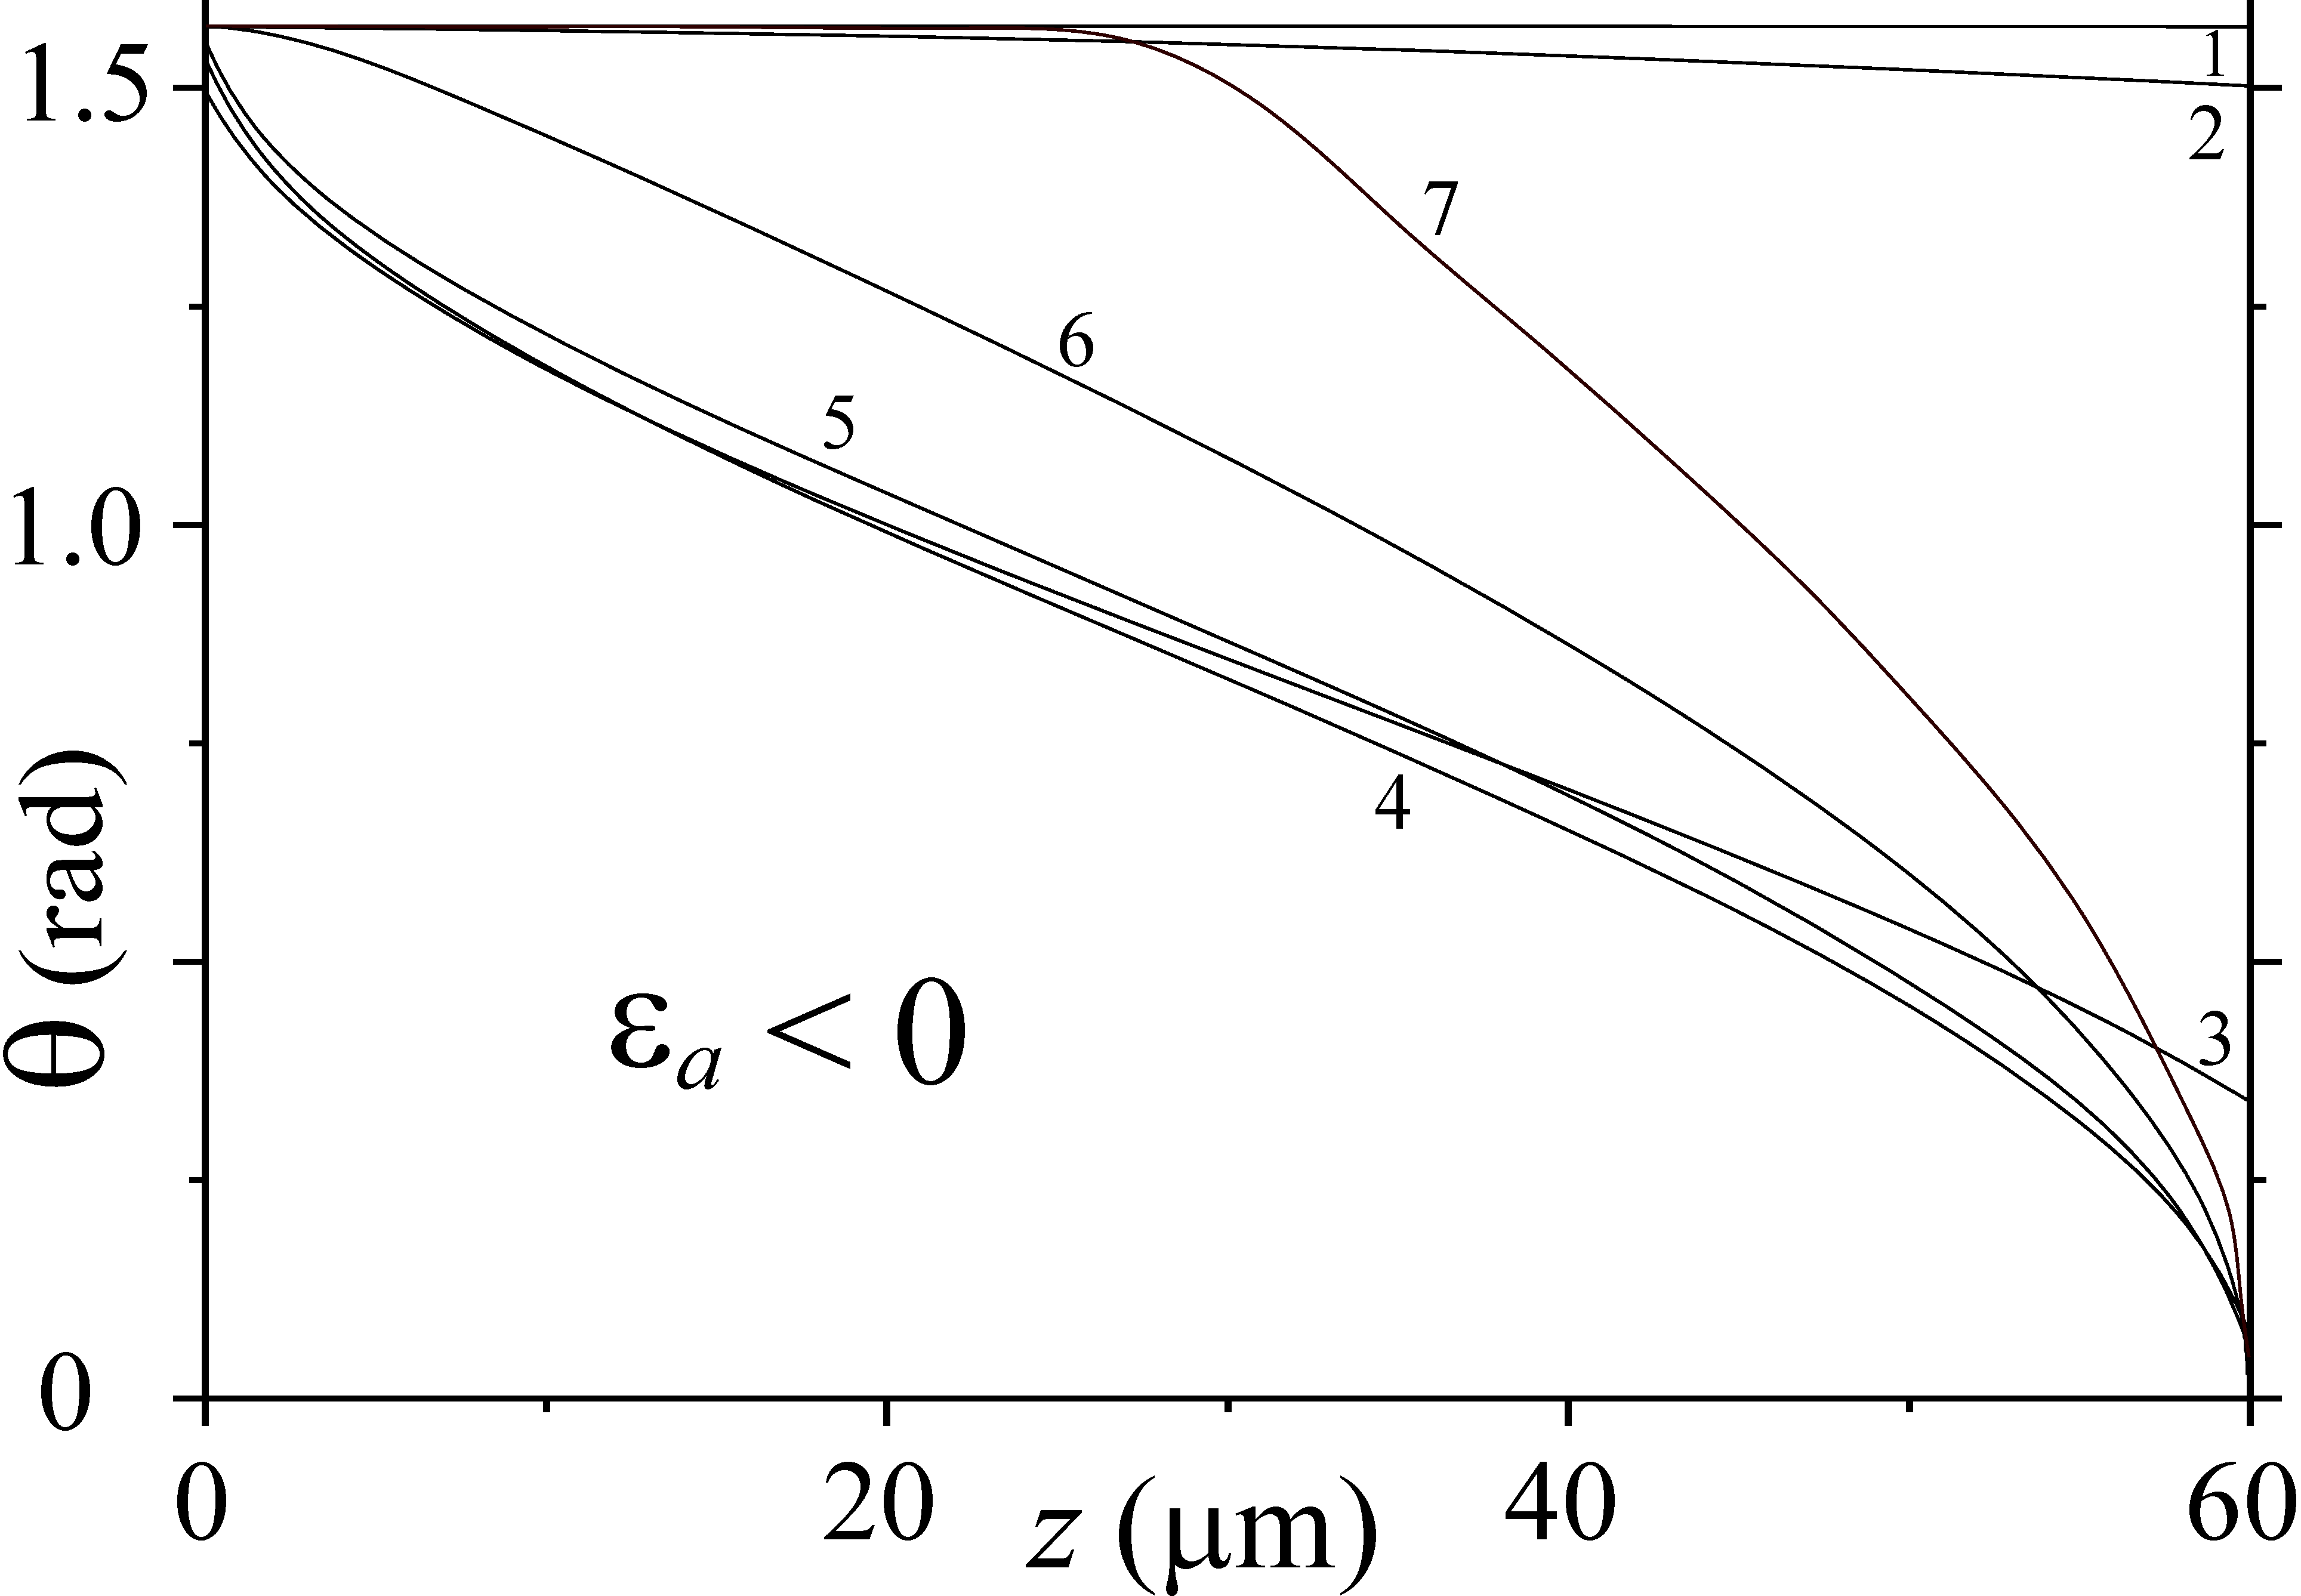
\includegraphics[width=0.48\textwidth]{Profiles_at_fixed_e_0_01_change_U.eps}%\\
	\hfill
	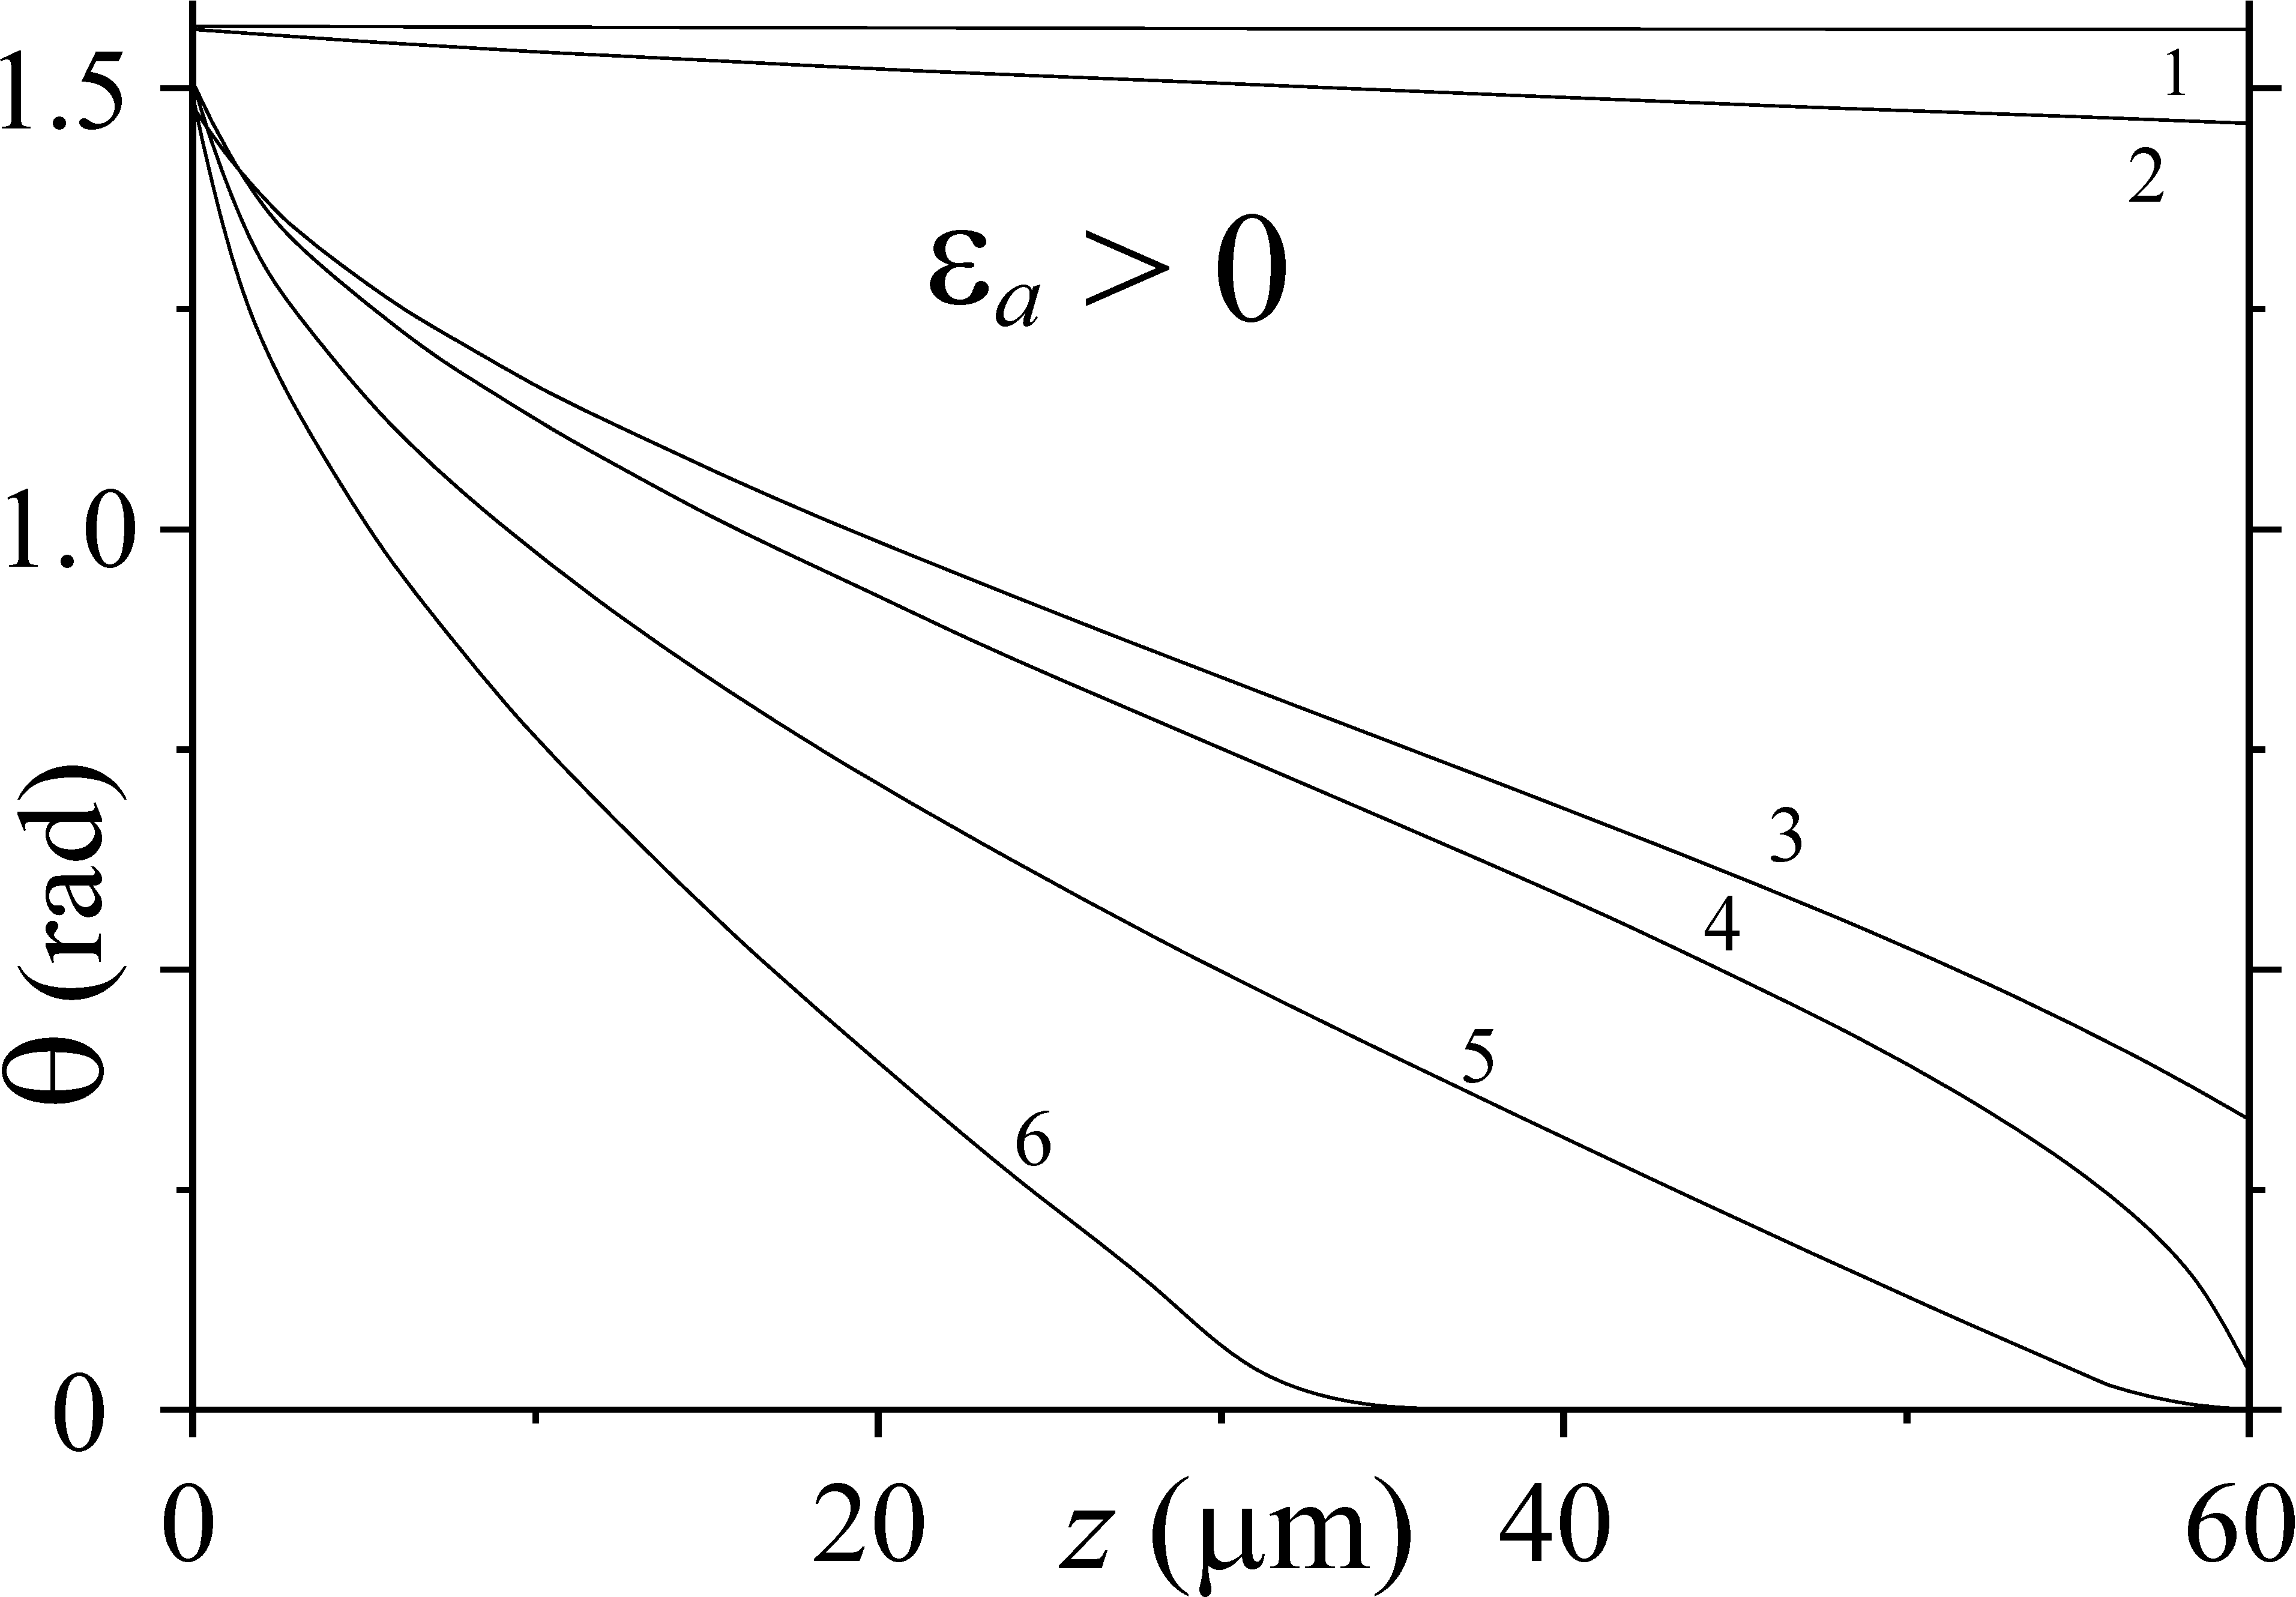
\includegraphics[width=0.48\textwidth]{Profiles_POSITIVE_EA_at_fixed_e_0_01_change_U.eps}
	\caption{Равновесная ориентационная структура $\theta(z)$ при $\bar{e}=0.01$~Фр/см. Напряжения для случая $\varepsilon_a<0$: 1 -- $U=0.15$~В, 2 -- $U = 0.17$~В, 3 -- $U = 0.18$~В, 4 -- $U = 1$~В, 5 -- $U = 2$~В, 6 -- $U = 5$~В и 7 -- $U = 10$~В; для случая $\varepsilon_a > 0$: 1 -- $U = 0.15$~В, 2 -- $U = 0.17$~В, 3 -- $U = 0.18$~В, 4 -- $U = 1$~В, 5 -- $U = 5$~В и 6 -- $10$~В.}\label{fig4_3}
\end{figure}
Отметим, что при очень высоком напряжении $U$ первое слагаемое в выражении~\eqref{eq_F_f_final123} становится определяющим.
Следовательно, система стремится к насыщенной ориентационной структуре, которая описывается зависимостью $\theta(z) = \pi/2$ при $\varepsilon_a < 0$ и $\theta(z) = 0$ при $\varepsilon_a > 0$.
Это можно пронаблюдать на Рис.~\ref{fig4_3} на примере профилей 5-7 для случая $\ve_a < 0$ и профилей 5 и 6 для случая $\ve_a > 0$.           % Глава 4
\chapter{Переход между искажёнными ориентационными структурами в случае большого усреднённого флексоэлектрического коэффициента.}\label{ch:ch5}
В предыдущей главе рассматривалась ситуация, когда при достаточно больших значениях $\bar{e}$ и $U$ выполнялось соотношение
\begin{equation}\label{criterion_eU}
\frac{\bar{e}U}{K}\gg 1,
\end{equation}
где $K = \max{K_{ii}}$ -- наибольший модуль Франка рассматриваемой системы.
При этом вкладами в свободную энергию $\FF_\mathrm{tot}$, даваемую выражением~\eqref{eq:free-energy}, содержащими $K_{ii}$ и $ W_\phi^{(1,2)}$, можно пренебречь.
Таким образом, выражение для свободной энергии может быть записано в следующем виде:
\begin{multline}\label{eq_F_f_final1_ch5}
\FF = \frac{S_\bot}{2} \bigg(-\frac{1}{4\pi}U^2 J + 2 \bar{e}U JJ_1 + 4\pi \bar{e}^2\int_{0}^{L}\frac{(\sin 2\theta \,\theta'-JJ_1)^2}{{\EE}(\theta)}dz +\\
+ W_\theta^{(1)} {\sin^2\big( \theta(0) - \theta_0^{(1)}\big)} + W_\theta^{(2)} {\sin^2\big( \theta(L) - \theta_0^{(2)}\big)}\bigg).
\end{multline}
Видно, что в этом пределе свободная энергия не зависит от азимутального угла $\phi(z)$, а значит, в этом случае нематические и холестерические ЖК описываются одинаково.

Исследуем, как равновесная ориентационная структура ЖК-ячейки (описываемая зависимостью $\theta(z)$) меняется в зависимости от приложенного напряжения $U$ для различных наборов материальных параметров.
В дальнейшем ограничимся углами лёгкого ориентирования на границах $\theta_0^{(1,2)} = \pi/2$.
Отметим, что в этом приближении свободная энергия~\eqref{eq_F_f_final1_ch5} является функционалом $\cos^2\theta(z)$.
Таким образом, удобно использовать замену $y(z)\equiv \cos^2\theta(z) + \ve_\bot/\ve_a = \EE(\theta)/\ve_a$.
Так как ранее мы указывали, что ищем функцию $\theta(z)\in C^2[0,\, L]$, то и на $y(z)$ накладываются такие же требования: $y(z)\in C^2[0,\, L]$. 
При этом важно, что функция $y(z)$ ограничена: $y(z)\in \left[{\ve_\bot}/{\ve_a},\ {\ve_\| }/{\ve_a}\right]\ \forall z\in[0,L]$.
Свободная энергия как функционал $y(z)$ имеет вид
\begin{multline}\label{eq_F_f_final_y}
\FF = \frac{S_\bot}{2}\bigg(-\frac{1}{4\pi}U^2 J + 2 \bar{e}U JJ_1 + \frac{4\pi \bar{e}^2}{\ve_a}\int_{0}^{L}\frac{(y'+JJ_1)^2}{y}dz +\\
+ W_\theta^{(1)}y(0) + W_\theta^{(2)}y(L) - (W_\theta^{(1)} + W_\theta^{(2)})\frac{\ve_\bot}{\ve_a}\bigg).
\end{multline}
В терминах $y(z)$ можно также записать
\begin{equation}\label{D_z=UJ_y}
J^{-1}= \ve_a^{-1}\int_0^L \frac{dz}{y},\quad J_1=\varepsilon_a^{-1}\ln\frac{y(0)}{y(L)}.
\end{equation}
Для того, чтобы рассчитать равновесную ориентационную конфигурацию $\theta(z)$, нужно найти функцию $y(z)$, доставляющую минимум функционалу~\eqref{eq_F_f_final_y}.
Так как функция $y(z)$ ограничена, необходимое условие минимизации свободной энергии можно сформулировать как неотрицательность её первой вариации
\begin{equation}
\delta \FF \geq 0.
\label{eq:dF1}
\end{equation}
Вариация $\delta\FF$ даётся следующей формулой:
\begin{equation}\label{eq:dF_ch5}
\begin{aligned}
\frac{\delta\FF}{S_\bot} = 
&\left[ \frac{-U^2 J^2}{8\pi} + \bar{e}U J_1 J^2 + 2\pi\bar{e}^2 \left( (y')^2 - 2y''y - J_1^2 J^2 \right) \right] \frac{\delta y(z)}{\ve_a y^2} + \\
&+\left[ \bar{e}UJ - 4\pi\bar{e}^2\left( y'(0) + JJ_1 \right) + \ve_a y(0) \frac{W_1}{2} \right] \frac{\delta y(0)}{\ve_a y(0)} + \\
&+\left[ -\bar{e}UJ + 4\pi\bar{e}^2\left( y'(L) + JJ_1 \right) + \ve_a y(L) \frac{W_2}{2} \right] \frac{\delta y(L)}{\ve_a y(L)}.
\end{aligned}
\end{equation}
При этом функция $y(z)$ должна удовлетворять условиям
\begin{subequations}
	\begin{empheq}[left = \empheqlbrace]{align}
		&0\leq z \leq L,\label{eq:rectangle_1}\\
		&\ve_\bot/\ve_a \leq y \leq \ve_\| /\ve_a.\label{eq:rectangle_2}
	\end{empheq}
\end{subequations}
\begin{figure}\label{pic:Allowed_areas_for_y}
	\centering
	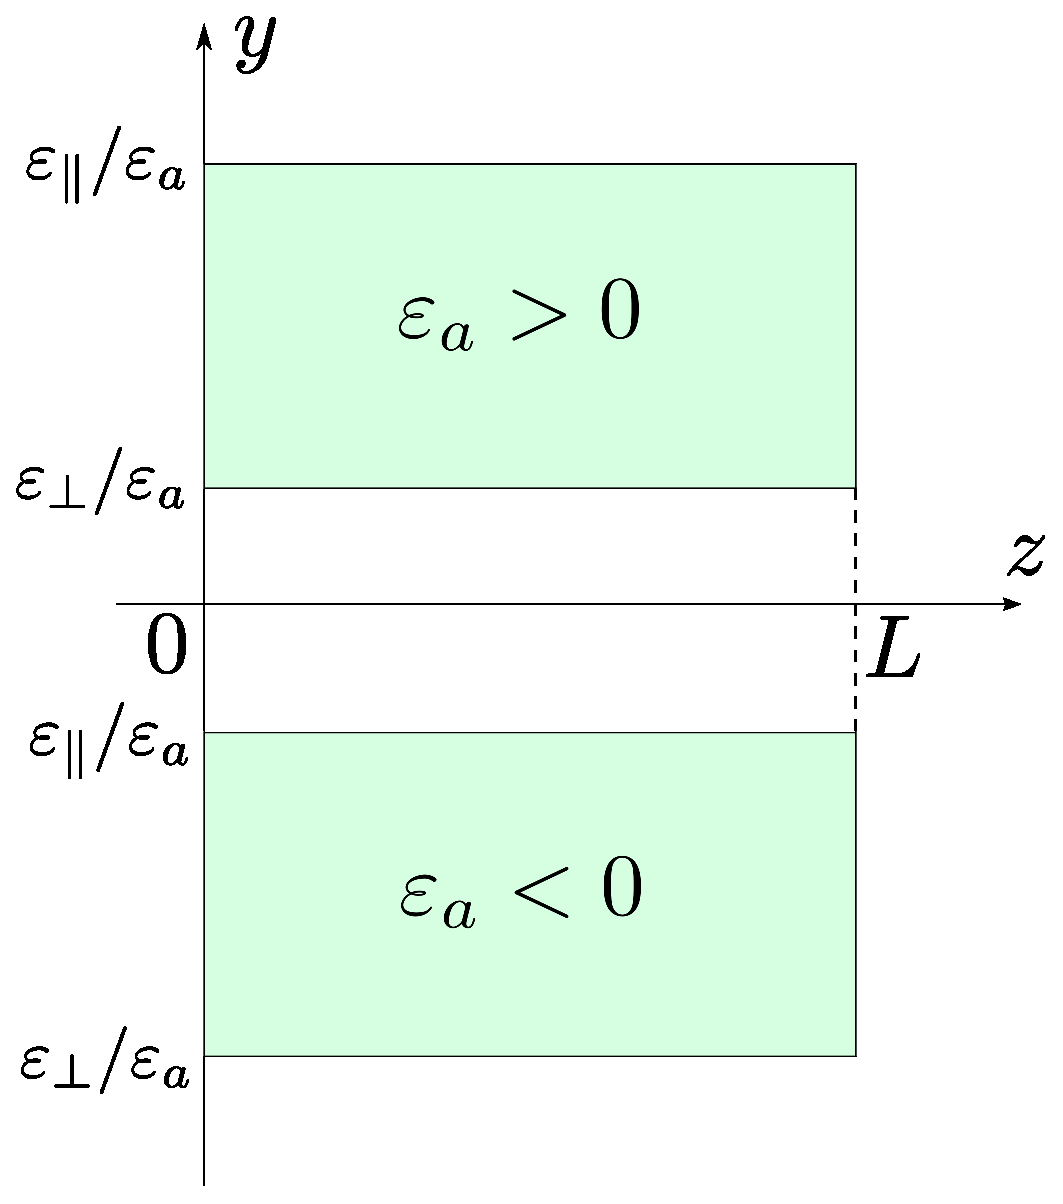
\includegraphics[width=0.55\textwidth]{Allowed_areas_for_y}
	\caption{Графическая иллюстрация системы неравенств~\eqref{eq:rectangle_1}  и~\eqref{eq:rectangle_2} для случаев $\varepsilon_a > 0$ и $\varepsilon_a < 0$.}
\end{figure}
На Рис.~\ref{pic:Allowed_areas_for_y} изображены области, задаваемые неравенствами~\eqref{pic:Allowed_areas_for_y}.
Таким образом, участок кривой $y(z)$ при $z\in[0,\, L]$ должен находиться внутри соответствующего прямоугольника.
Минимум функционалу могут доставлять и такие профили, у которых существуют точки или целые области, где $y(z) = \ve_\|/\ve_a$ или $y(z) = \ve_\bot/\ve_a$.
Обозначим множество таких точек через $A$, а дополнение $A$ до отрезка $[0,L]$ -- $B$.
Проиллюстрируем эти множества на примере графика зависимости $y(
z)$, приведённого на Рис.~\ref{pic:Sample_profile}.
\begin{figure}\label{pic:Sample_profile}
	\centering
	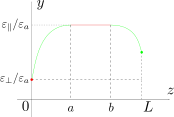
\includegraphics[width=0.7\textwidth]{Sample_profile}
	\caption{График зависимости $y(z)$, иллюстрирующий случай, когда кривая $y(z)$ касается границ ограничивающего прямоугольника.}
\end{figure}
Так, в данном случае $A = \{0\}\cup[a,b]$, $B = (0,a)\cup(b,L]$.
Также важно отметить, что бесконечно малые вариации $\delta y(z)$ произвольны, когда $z\in B$.
В этом случае в условии~\eqref{eq:dF1} может реализоваться только равенство.
Это требование приводит к следующему уравнению Эйлера-Лагранжа:
\begin{align}\label{eq:E-l_y}
&-2yy''+(y')^2 - J^2\left(J_1 - \frac{U}{4\pi\bar{e}}\right)^2 = 0%\\
%&\ve_\bot/\ve_a < y(z) < \ve_\| /\ve_a, \label{cond10}\\
%&0 < z < L.
\end{align}
и граничными условиями
\begin{subequations}
	\begin{align}
		&\bar{e}UJ - 4\pi\bar{e}^2\left( y'(0) + JJ_1 \right) + \ve_a y(0) \frac{W_1}{2} = 0 \label{eq:ch5_boundary1_eq}\\
		-&\bar{e}UJ + 4\pi\bar{e}^2\left( y'(L) + JJ_1 \right) + \ve_a y(L) \frac{W_2}{2} = 0.\label{eq:ch5_boundary2_eq}
	\end{align}
\end{subequations}
Однако при достижении $y(z)$ "верхней" или "нижней" границы прямоугольника~\eqref{eq:rectangle_2}, то есть когда $z\in A$, эти вариации оказываются знакоопределёнными: $\delta y(z) \geq 0$, если $y(z) = \ve_\bot/\ve_a$, и $\delta y(z) \leq 0$ при $y(z) = \ve_\| /\ve_a$.
В этом случае, используя выражение для первой вариации свободной энергии~\eqref{eq:dF_ch5}, для $z\in(0,\ L)\cap A$ вместо уравнения Эйлера-Лагранжа~\eqref{eq:E-l_y} можно записать неравенство
\begin{equation}\label{eq:E-l_ineq}
\left(-2yy''+(y')^2 - J^2\left(J_1 - \frac{U}{4\pi\bar{e}}\right)^2\right)\frac{\delta y}{y} \ge 0.
\end{equation}
Для $z\in \{0, L\}\cap A$ граничные условия также примут форму неравенств:
\begin{subequations}
	\begin{align}
		\left[ -y'(0) - J\left(J_1  - \frac{U}{4\pi\bar{e}}\right) + g_1 y(0) \right]\delta y(0) &\geq 0,\label{eq:boundary1_ch5}\\
		\left[ y'(L) + J\left(J_1  - \frac{U}{4\pi\bar{e}}\right) + g_2 y(L) \right]\delta y(L) &\geq 0,\label{eq:boundary2_ch5}
	\end{align}
\end{subequations}
где
\begin{equation}
g_i = \frac{\ve_a W_i}{8\pi\bar{e}^2},\quad i = 1,2.
\end{equation}
Утверждение.
Если существует некоторый отрезок $[a,\ b] \subset(0,L)$ такой, что множество $[a,b]\cap A$ содержит конечное число элементов, то во всех этих точках $\delta \FF/\delta y = 0$.
Действительно, пусть нашёлся такой отрезок $[a,\ b]$, что существует $z_1$: $z_1\in[a,\ b]\cap A$.
Тогда из непрерывности $\delta \FF/\delta y(z)$ следует, что
\begin{equation}
\frac{\delta \FF}{\delta y(z_1-0)} = \frac{\delta \FF}{\delta y(z_1+0)} = \frac{\delta \FF}{\delta y(z_1)}.
\end{equation}
При этом хотя бы с одной из сторон от $z_1$ $\delta\FF/\delta y(z) = 0$ в силу определения отрезка $[a,\ b]$.
Слеовательно, значение вариации в точке $z_1$ также нулевое.
Утверждение доказано.
	
%Отдельно отметим, что для $z\in\partial A\cap (0,\ L)$ в~\eqref{eq:E-l_ineq} должно выполняться равенство (по непрерывности), а для $z\in\interior{A}$ -- неравенство. 
%Необходимые условия минимума свободной энергии также включают в себя ледующие граничные условия:
%Здесь строгое неравенство соответствует случаю, когда $\{0\}\in A$ или $\{ L \}\in A$, в противном случае имеет место равенство.
При записи условий~\eqref{eq:E-l_ineq}, \eqref{eq:boundary1_ch5} и~\eqref{eq:boundary2_ch5} учтено, что $\ve_a y(z) = \EE(\theta(z)) > 0$.
Отметим, что неравентва~\eqref{eq:E-l_ineq}--\eqref{eq:boundary2_ch5} аналогичны условиям Каруша-Куна-Таккера (см., например,~\cite{Kun-TakkerBook}) для уравнения Эйлера-Лагранжа с граничными условиями.
Таким образом, поиск равновесной ориентационной структуры ЖК-ячейки сводится к достаточно необычной математической задаче: уравнение Эйлера-Лагранжа~\eqref{eq:E-l_y} является интегро-дифференциальным, а также содержит значения искомой функции на границах.
Каждое из граничных условий~\eqref{eq:boundary1_ch5} и~\eqref{eq:boundary2_ch5} -- неравенство и тоже содержит интегральный множитель $J$, зависящий от распределения $\theta(z)$ в объёме ячейки, а также значения $y(0)$ и $y(L)$ в множителе $J_1$.
Наконец, условие, которому должна удовлетворять искомая функция $y(z)$, может быть различным и зависит от того, как распределяются множества $A$ и $B$ на отрезке $[0,\ L]$ для конкретной функции-кандидата. 
%Наконец, если происходит касание границ~\eqref{eq:y_border}, уравнение Эйлера-Лагранжа заменяются неравенством~\eqref{eq:E-l_ineq}.

Достаточное условие минимума свободной энергии может быть получено, если добавить к~\eqref{eq:dF1} требование положительности второй вариации свободной энергии
\begin{equation}
\delta^2\FF[y(z)] > 0,\quad z\in B\cup(\partial A\cap (0,\ L)).
\end{equation}
Во всех остальных точках отрезка $[0,\ L]$ достаточное условие даётся неравенством~\eqref{eq:E-l_ineq}.

Для решения уравнения Эйлера-Лагранжа введём обозначение
\begin{equation}\label{eq:parameter_a}
a = J\left(J_1 - \frac{U}{4\pi\bar{e}}\right).
\end{equation}
Так как выражение $J(J_1 - U/(4\pi\bar{e}))$ не зависит от $z$, получаем параметрическое уравнение
\begin{equation}\label{eq:parametric_EL}
-2yy''+(y')^2 - a^2 = 0.
\end{equation}
Этот параметр также входит в граничные условия~\eqref{eq:boundary1_ch5} и~\eqref{eq:boundary2_ch5}.

Заметим, что если вторая производная  $y''$ равна нулю (а значит, $y(z)$ -- линейная функция), то уравнение~\eqref{eq:parametric_EL} принимает вид
\begin{equation}
(y')^2 - a^2 = 0.
\end{equation}
Семейство линейных функций, являющихся его решениями, может быть описано как
\begin{equation}
y(z) = \pm az + b,
\end{equation}
где $b$ -- произвольная константа.

Далее, путь $y'' \neq 0$.
Введём замену $\tau(y) = y'$.
Тогда справедлива цепочка равенств
\begin{equation}\label{eq:tau_ch5}
y''_{zz} = \tau'_z = \tau'_y y' = \tau'_y\tau.
\end{equation}
Подставляя выражение для $y''$ из~\eqref{eq:tau_ch5} в~\eqref{eq:parametric_EL}, получаем:
\begin{equation}
-2y\tau'_y\tau + \tau^2 - a^2 = 0.
\end{equation}
Разделив переменные и проинтегрировав, запишем
\begin{equation}
\tau^2 - a^2 = cy,
\end{equation}
где $c$ -- произвольная константа.
Учитывая, что $\tau = y'$, проинтегрируем это уравнение:
\begin{equation}
|y'| = \sqrt{cy + a^2} \Rightarrow y = \frac{c}{4}\left( z + b \right)^2- \frac{a^2}{c}.
\end{equation}
Здесь $b$ -- также произвольная константа.

Таким образом, уравнение~\eqref{eq:parametric_EL} имеет три независимых решения
\begin{align}
&y(z) = \pm az + b,\label{eq:linear_solution}\\
&y(z) = \frac{c}{4}\left(z+b\right)^2 - \frac{a^2}{c},\label{eq:parabolic_solution}
\end{align}
где $b$ и $c$ -- произвольные константы.
Выражение~\eqref{eq:parameter_a} является, по своей сути, условием самосогласования на параметр $a$, так как $J$ и $J_1$, в свою очередь, зависят от $a$.
\section{Линейное решение}\label{sec:sec5.1}
Отметим, что из-за требования $y\in C^2[0,\, L]$ кусочно-заданная функция, состоящая из линейных функций~\eqref{eq:linear_solution} решением быть не может.
Подставляя линейное решение~\eqref{eq:linear_solution} в уравнение~\eqref{eq:parametric_EL}, приходим к следующему равенству:
\begin{equation*}
\frac{JU}{4\pi\bar{e}} = 0.
\end{equation*}
Это требование может быть выполнено только в тривиальном случае $U = 0$.
Таким образом, в дальнейшем будем рассатривать только параболическое решение~\eqref{eq:parabolic_solution} с учётом ограничения~\eqref{eq:rectangle_2} на $y(z)$.
Это требование совместно с условиями на границах ячейки~\eqref{eq:boundary1_ch5} и~\eqref{eq:boundary2_ch5}, а также условием самосогласования~\eqref{eq:parameter_a} позволяет определить параметры $a$, $b$ и $c$.
\section{Параболическое решение без участков насыщения}
Проверим возможность существования параболического решения $y(z)$ вида~\eqref{eq:parabolic_solution}, для которого было бы выполнено условие $y(z) \in (\ve_\|/\ve_a,\, \ve_\bot/\ve_a) \forall z\in[0,\, L]$.
На языке множеств $A$ и $B$ этот случай соответствует пустому множеству $B$.
Решение должно обладать следующими свойствами:
\begin{itemize}
	\item Абсцисса вершины параболы находится либо вне отрезка $[0,\, L]$, либо её ордината лежит в области возможных значений функции $y(z)$:
	\begin{subequations}
		\begin{empheq}[left = \empheqlbrack]{align}
			&-b \notin [0,\, L],\\
			&\frac{\ve_\bot}{\ve_a}< \frac{-a^2}{c} < \frac{\ve_\|}{\ve_a};
		\end{empheq}
	\end{subequations}
	\item Значения функции $y(z)$ на краях отрезка $[0,\, L]$ также должны находиться в указанном выше интервале:
	\begin{equation}
		\ve_\bot / \ve_a < y(0,\, L) < \ve_\| / \ve_a
	\end{equation}
	\item Должны быть удовлетворены граничные условия~\eqref{eq:ch5_boundary1_eq} и~\eqref{eq:ch5_boundary2_eq};
	\item Должно выполняться условие самосогласования~\eqref{eq:parameter_a}.
\end{itemize}
Подставим исследуемое параболическое решение в граничные условия~\eqref{eq:ch5_boundary1_eq} и~\eqref{eq:ch5_boundary2_eq} и после несложных преобразований получим:
\begin{subequations}
	\begin{align}
		&\left( b + \frac{2a}{c} \right)\left( \frac{g_1}{2}(b - \frac{2a}{c}) - 1 \right) = 0\label{eq:ch5_boundary1_1}\\
		&\left( L + b + \frac{2a}{c} \right)\left( \frac{g_2}{2}(L + b - \frac{2a}{c}) - 1 \right) = 0.\label{eq:ch5_boundary2_1}
	\end{align}
\end{subequations}
Кроме того, вычисляя $J$ и $J_1$ для $y(z)$ заданного вида, запишем условие самосолгасования~\eqref{eq:parameter_a}:
\begin{multline}
a = a \ve_a \left(\ln{\left( \frac{L+b - 2a/c}{b - 2a/c} \times \frac{b+ 2a/c}{L+b+2a/c} \right)} \right)^{-1} \times\\
\times \left( \frac{1}{\ve_a}\ln{ \left( \frac{b - 2a/c}{L + b - 2a/c} \times \frac{b+ 2a/c}{L+b+2a/c} \right)} - \frac{U}{4\pi\bar{e}} \right).
\end{multline}
После преобразований получаем следующее условие:
\begin{equation}\label{eq:ch5_gamma_1}
	L + b - \frac{2a}{c} = \gamma\left( b - \frac{2a}{c} \right).
\end{equation}
Здесь и далее использовано обозначение
\begin{equation}
	\gamma = \exp{\left(\frac{-\ve_a U}{8\pi\bar{e}}\right)}.
\end{equation}
Видно, что условия~\eqref{eq:ch5_boundary1_1} и~\eqref{eq:ch5_boundary2_1} приводят к равенству нулю одного из множителей в каждом условии.
Рассмотрим теперь значения функции $y(z)$ на границах ячейки:
\begin{subequations}
	\begin{align}
		&y(0) = \frac{c}{2}\left( b-\frac{2a}{c} \right)\left( b + \frac{2a}{c} \right)\\
		&y(L) = \frac{c}{2}\left( L + b - \frac{2a}{c} \right)\left( L + b + \frac{2a}{c} \right)
	\end{align}
\end{subequations}
Из того, что они должны быть отличны от нуля, следует, что в условиях~\eqref{eq:ch5_boundary1_1} и~\eqref{eq:ch5_boundary2_1} нулю могут быть равны только вторые множители, что приводит к следующим равенствам:
\begin{align}
&b - 2a/c = 2/g_1\label{eq:ch5_boundary1_2}\\
&L + b - 2a/c = 2/g_2.\label{eq:ch5_boundary2_2}
\end{align}
Видно, что подстановка~\eqref{eq:ch5_boundary1_2} и~\eqref{eq:ch5_boundary2_2} в~\eqref{eq:ch5_gamma_1} даёт
\begin{equation}
g_1 = \gamma g_2.
\end{equation}
Это выражение связывает материальные параметры и не может быть удовлетворено в общем случае.

Рассмотрим решение параболического типа, для которого множество $B$ содержит единственную точку $z_0$.
Как было показано ранее, если эта точка находится на интервале $(0,\, L)$, то уравнение Эйлера-Лагранжа остаётся в силе, а значит, ничего, по сравнению с предыдущим рассмотренным случаем не меняется.
Таким образом, имеет смысл рассмотреть ситуацию, когда $z_0 = 0$ или $z_0 = L$.
Если эта точка находится на левой границе, $z_0 = 0$, то рассмотрим совместно выражение~\eqref{eq:ch5_gamma_1}, возникающее из условия самосогласования, и равенство~\eqref{eq:ch5_boundary2_2}, возникающее из граничного условия~\eqref{eq:ch5_boundary1_2}:
\begin{subequations}
	\begin{align}
		&L+b-\frac{2a}{c} = \frac{2}{g_2}\\
		&L + b - \frac{2a}{c} = \gamma \left(b - \frac{2a}{c}\right).
	\end{align}
\end{subequations}
Выражая $b - 2a/c$ из каждого из условий и приравнивая полученное, запишем:
\begin{equation}
\frac{2}{g_2} - L = \frac{L}{\gamma - 1}.
\end{equation}
Вновь получено равенство, связывающее материальные параметры, а значит, решение такого типа невозможно. Аналогично можно доказать, что случай $z_0 = L$ тоже не реализуется.

Таким образом, для случая чисто параболического решения остаётся рассмотреть ситуацию, когда на обеих границах отрезка $[0,\, L]$ $y(z)\in\{ \ve_\bot / \ve_a,\, \ve_\| / \ve_a \}$.
Введём обозначения
\begin{equation}
	y(0,\, L) = \mu_{0,\, L}.
\end{equation}
Можно записать все условия, которым должно удовлетворять решение:
\begin{subequations}
	\begin{empheq}[left = \empheqlbrace]{align}
		&y(z) = \frac{c}{4}(z + b)^2 - \frac{a^2}{c},\label{eq:ch5_parabolic_system_1}\\
		&y(0) = \mu_0,\label{eq:ch5_parabolic_system_2}\\
		&y(L) = \mu_L,\label{eq:ch5_parabolic_system_3}\\
		&a = J\left(J_1 - \frac{U}{4\pi\bar{e}}\right),\label{eq:ch5_parabolic_system_4}\\
		&\left[\begin{aligned}
			&-b \notin [0,\, L],\\
			&\frac{\ve_\bot}{\ve_a}< \frac{-a^2}{c} < \frac{\ve_\|}{\ve_a},
		\end{aligned}\right.,\label{eq:ch5_parabolic_system_5}\\
		&\left[ -(y'(0) + a) + g_1 y(0) \right]\delta y(0) \geq 0,\label{eq:ch5_parabolic_system_6}\\
		&\left[ y'(L) + a + g_2 y(L) \right]\delta y(L) \geq 0.\label{eq:ch5_parabolic_system_7}
	\end{empheq}
\end{subequations}
Подстановка зависимости~\eqref{eq:ch5_parabolic_system_1} в~\eqref{eq:ch5_parabolic_system_2}, \eqref{eq:ch5_parabolic_system_3} и~\eqref{eq:ch5_parabolic_system_4} даёт следующую систему уравнений на коэффициенты $a$, $b$ и $c$: \todo{(эта система взята со страницы R-2)}
\begin{subequations}
	\begin{empheq}[left = \empheqlbrace]{align}
		&b = -\frac{L}{2}\left( \frac{\pm \gamma}{\frac{\mu_L}{\mu_0} \pm \gamma} + \frac{1}{1\pm \gamma} \right),\\
		&b - \frac{2a}{c} = \frac{-L}{1 \pm \gamma},\\
		&\frac{c}{4} \cdot \frac{-L}{1 \pm \gamma}\left( b + \frac{2a}{c} \right) = \mu_0.
	\end{empheq}
\end{subequations}
Здесь и далее подразумевается, что во всех выражениях могут стоять одновременно либо только ``верхние'', либо только ``нижние'' знаки.
После несложных алгебраических преобразований удаётся выразить следующие конструкции из коэффициентов, удобные для дальнейшей подстановки:
\begin{subequations}\label{eq:ch5_parabolic_coeff_system}
	\begin{empheq}[left = \empheqlbrace]{align}
		&b = \frac{-L}{2}\left( \frac{\pm \gamma}{\frac{\mu_L}{\mu_0} \pm \gamma} + \frac{1}{1 \pm \gamma}\right),\label{eq:ch5_parabolic_coeff_system_1}\\
		&\frac{2a}{c} = \frac{L}{2}\left( \frac{1}{1 \pm \gamma} - \frac{\pm \gamma}{\frac{\mu_L}{\mu_0} \pm \gamma} \right),\label{eq:ch5_parabolic_coeff_system_2}\\
		&\frac{c}{4} = \frac{\mu_0 \left(1 \pm \gamma\right)\left( \frac{\mu_L}{\mu_0} \pm \gamma \right)}{\pm \gamma L^2}.\label{eq:ch5_parabolic_coeff_system_3}
	\end{empheq}
\end{subequations}
Граничные условия~\eqref{eq:ch5_parabolic_system_6} и~\eqref{eq:ch5_parabolic_system_7} после подстановки в них выражений для коэффициентов~\eqref{eq:ch5_parabolic_coeff_system_1} -- \eqref{eq:ch5_parabolic_coeff_system_3} принимают следующий вид:
\begin{subequations}\label{eq:ch5_some_system}
	\begin{empheq}[left = \empheqlbrace]{align}
		&\mu_0\left( g_1 + \frac{2(1 \pm \gamma)}{L} \right) \delta y(0) \geq 0,\label{eq:ch5_some_system_a}\\
		&\mu_L \left( g_2 + \frac{2(1 \pm \gamma^{-1})}{L} \right) \delta y(L) \geq 0.\label{eq:ch5_some_system_b}
	\end{empheq}
\end{subequations}
\todo{АО: надо придумать, как здесь заменить $\delta y(0,\, L)$ на единицу в некоторой степени.}
Для того, чтобы анализа полученные неравенства, необходимо выбрать знаки $\ve_a$ и $U$.
Произведём расчёт для случая $\ve_a > 0$, $U > 0$.
Заметим, что в этом случае выполнены следующие неравества:
\begin{subequations}
	\begin{align}
		&\mu_{0,L} > 0,\label{eq:ch5_conseq_from_positive_ea_U_1}\\
		&0 < \gamma \leq 1,\label{eq:ch5_conseq_from_positive_ea_U_2}\\
		&1 \leq \gamma^{-1} < \infty.\label{eq:ch5_conseq_from_positive_ea_U_3}
	\end{align}
\end{subequations}
Учитывая требование~\eqref{eq:ch5_conseq_from_positive_ea_U_2}, неравенство~\eqref{eq:ch5_some_system_a} можно свести к требованию $\delta y(0) > 0$, что соответствует $\mu_0 = \ve_\bot / \ve_a$.
Предположим, что знак при $\gamma$ -- ``верхний''.
Тогда неравенство~\eqref{eq:ch5_some_system_b} принимает вид
\begin{equation}
	\left( g_2 + \frac{2(1 + \gamma^{-1})}{L} \right) \delta y(L) \geq 0.
\end{equation}
Выражение в скобках может принимать только положительные значения ($g_{1,2} > 0$, так как $\ve_a > 0$).
Таким образом, приходим к требованию $\delta y(L) > 0$, что соответствует $\mu_L = \mu_0 = \ve_\bot / \ve_a$.
Так как $y(0) = y(L)$, вершина параболы находится в точке $z = L/2$, а значит, нужно проверить, не выходит ли ордината вершины за границы допустимого отрезка.
Выражение для ординаты параболы:
\begin{equation}\label{eq:ch5_ordinate_of_vertex_symmetric}
	y(z)\bigg|_{z = -b} = \frac{-a^2}{c},
\end{equation}
на него наложено следующее ограничение:
\begin{equation}\label{eq:ch5_case1_ineq_system}
	\frac{\ve_\bot}{\ve_a} \leq \frac{-a^2}{c} \leq \frac{\ve_\|}{\ve_a}.
\end{equation}
Воспользуемся полученными ранее формулами~\eqref{eq:ch5_parabolic_coeff_system}, чтобы выразить $-a^2/c$, и после несложных преобразований получим
\begin{equation}\label{eq:ch5_case_low_sign_ineq}
	1 \leq \frac{-(1 - \gamma)^2}{4\gamma}\leq \frac{\ve_\|}{\ve_\bot}.
\end{equation}
Видно, что это условие не выполняется, а значит, решений в случае выбранного при $\gamma$ знака при $\ve_a > 0$ и $U > 0$ нет.

Рассмотрим теперь ``нижний'' знак при $\gamma$.
В этом случае неравенство~\eqref{eq:ch5_some_system_b} принимает вид
\begin{equation}\label{eq:ch5_right_border_ineq}
	\left( g_2 + \frac{2(1 - \gamma^{-1})}{L} \right) \delta y(L) \geq 0.
\end{equation}
Знак выражения в скобках определяет, какого знака должна быть вариация $\delta y(L)$.
Заметим, что с ростом $U$ значение $\gamma^{-1}$ также монотонно растёт.
Следовательно, существует некоторое значение напряжения $U = \tilde{U}$ такое, что при $U < \tilde{U}$, $\delta y(L) > 0$, а при $U > \tilde{U}$, $\delta y(L) < 0$.
Найти напряжение $\tilde{U}$ можно, приравнивая значение выражения в скобках в формуле~\eqref{eq:ch5_right_border_ineq} к нулю.
После несложных преобразований получим:
\begin{equation}
	\tilde{U} = \frac{8\pi \bar{e}}{\ve_a} \ln \left( 1 + \frac{\ve_a W_2 L}{16\pi \bar{e}^2} \right).
\end{equation}
Рассмотрим случай  $U < \tilde{U}$.
Как сказано выше, это условие приводит к тому, что $\mu_L = \ve_\bot / \ve_a$.
Проверим, выполняется ли условие на ординату вершины параболы, которая при $\mu_0 = \mu_L$ имеет абсциссу $z = -b$.
Подставим в~\eqref{eq:ch5_ordinate_of_vertex_symmetric} выражения для комбинации коэффициентов из~\eqref{eq:ch5_parabolic_coeff_system}:
\begin{equation}
	y(z)\bigg|_{z = -b} = -\left( \frac{2a}{c} \right)^2 \cdot \frac{c}{4} = \frac{\mu_0 \left( \frac{\mu_L}{\mu_0} - \gamma^2 \right)^2}{4\gamma\left(1-\gamma\right)\left( \frac{\mu_L}{\mu_0} - \gamma \right)}.
\end{equation}
Подставляя полученные выше значения $\mu_0 = \mu_L = \ve_\bot / \ve_a$, запишем условие на вершину параболы:
\begin{equation}\label{eq:ch5_toomanynames_001}
	1 \leq \frac{(1+\gamma)^2}{4\gamma} \leq \frac{\ve_\|}{\ve_\bot}.
\end{equation}
Видно, что первое неравенство в~\eqref{eq:ch5_toomanynames_001} выполнено для всех $\gamma\in(0,\, 1]$, а вот второе является содержательным.
Исследуем неравенство
\begin{equation}\label{eq:ch5_case_1_ineq}
(1+\gamma)^2 \leq \frac{4\gamma\ve_\|}{\ve_\bot}.
\end{equation}
Графики функций $f_1(\gamma) = (1+\gamma)^2$ и $f_2(\gamma) = 4\gamma\ve_\|/\ve_\bot$ представлены на Рис.~\ref{fig:ch5_graph_solver_1}
\begin{figure}[h]
	\centering
	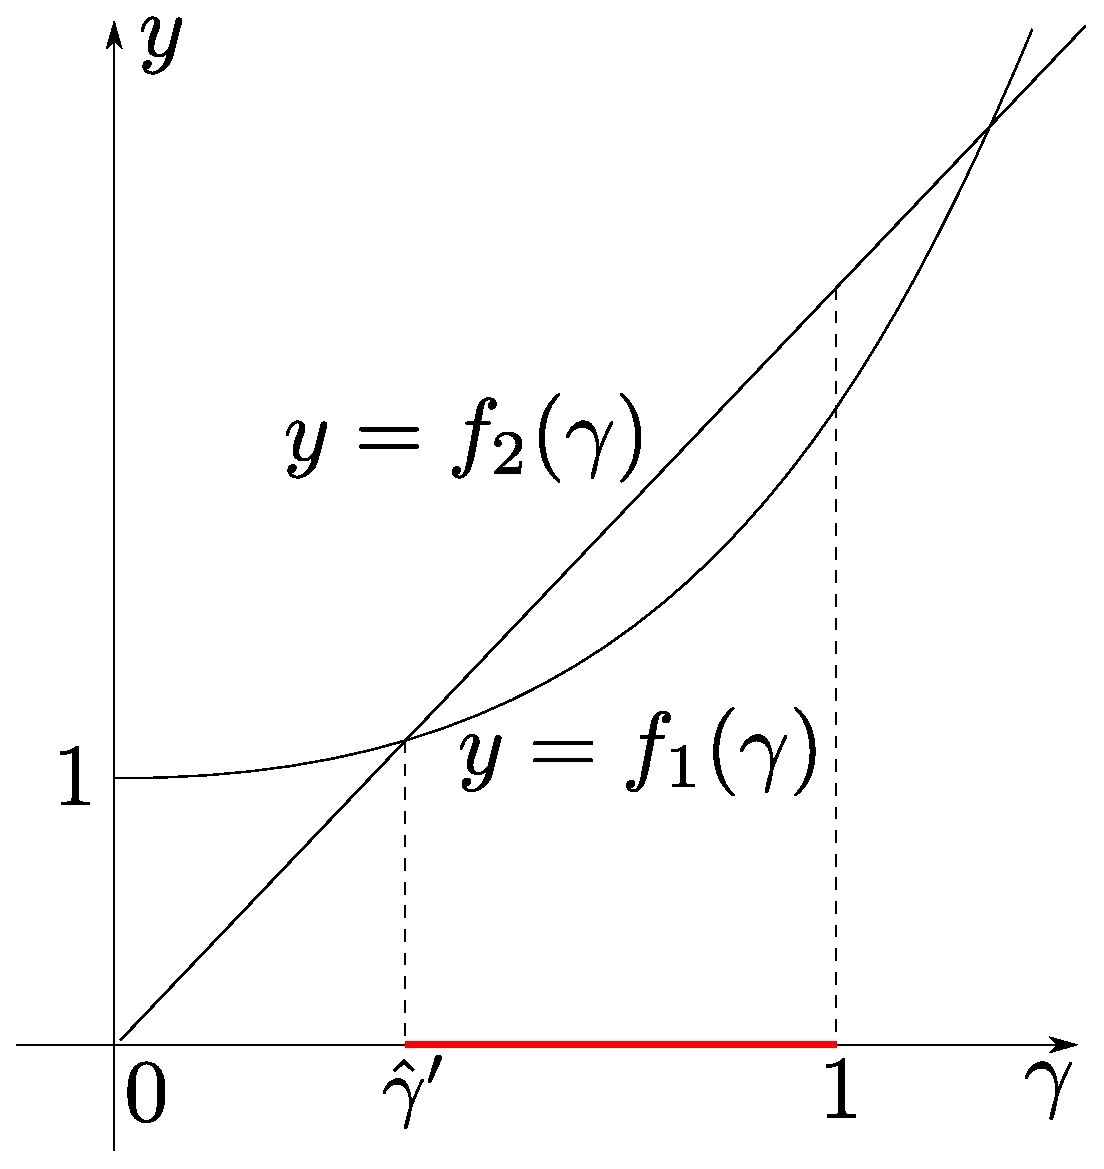
\includegraphics[width=20pc]{ch5_graph_solver_1.eps}
	\caption{Графики функций $y = f_1(\gamma)$ и $y = f_2(\gamma)$. Цветом выделен участок на оси $\gamma$, соответствующий решению неравенства~\eqref{eq:ch5_case_1_ineq}.}\label{fig:ch5_graph_solver_1}
\end{figure}
При построении графиков учтено, что $f_2(0) < f_1(0)$ и $f_2(1) > f_1(1)$, следовательно, на интервале $(0,\, 1)$ существует $\hat{\gamma}'$ такая, что $f_1(\hat{\gamma}') = f_2(\hat{\gamma}')$.
При этом неравенство~\eqref{eq:ch5_case_1_ineq} выполнено при $\hat{\gamma}' < \gamma \leq 1$, что в терминах напряжений соответствует $0 \leq U < \hat{U}'$, $\hat{U}':\hat{\gamma}' = \gamma(\hat{U}')$.
Приведём точное выражение для $\hat{\gamma}'$ и соответствующего напряжения $\hat{U}'$:
\begin{align}
	&\hat{\gamma}' = \frac{2\ve_\|}{\ve_\bot} - 1 - \frac{2\ve_\|}{\ve_\bot} \sqrt{\frac{\ve_a}{\ve_\|}},\\
	&\hat{U}' = \frac{8\pi\bar{e}}{\ve_a}\ln\left( \frac{1}{\hat{\gamma}'} \right).
\end{align}
Напомним, что условие $U < \tilde{U}$ соответствует неравенству, заменяющему граничное условие на границе $z = L$, а условие $U < \hat{U}'$ соответствует требованию, чтобы вершина параболы не выходила за гарницы обозначенного прямоугольника.

Таким образом, заключаем, что при $U < \min(\tilde{U},\,\hat{U}_1)$ возможно существование профиля, изображённого на Рис.~\ref{fig:ch5_profile_1}.
\begin{figure}
	\centering
	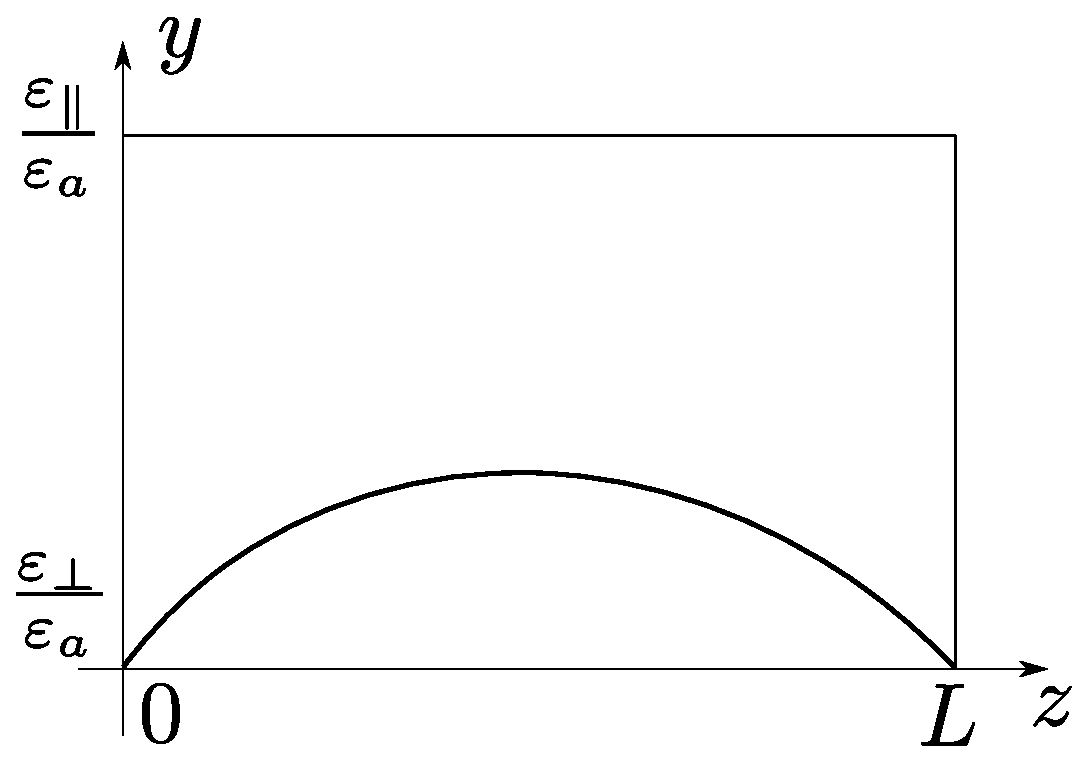
\includegraphics[width = 17pc]{ch5_profile_1.eps}
	\caption{Вид профиля при напряжении $U < \min(\tilde{U},\,\hat{U}_1)$}\label{fig:ch5_profile_1}
\end{figure}
Подставляя $\mu_0 = \mu_L = \ve_\bot/\ve_a$ в~\eqref{eq:ch5_parabolic_coeff_system} и выбирая ``нижний'' знак при $\gamma$, можно получить уравнение такого профиля:
\begin{equation}\label{eq:ch5_simple_parabolic_profile}
	y(z) = \frac{\ve_\bot}{\ve_a}\cdot\frac{(1 - \gamma)^2}{-\gamma^2}\cdot\left( \frac{z}{L}  - \frac{1}{2} \right)^2 + \frac{\ve_\bot}{\ve_a}\cdot \frac{(1 + \gamma)^2}{4\gamma}
\end{equation}

Мы рассмотрели случай $U < \tilde{U}$, что приводит к $\mu_L = \ve_\bot / \ve_a$.
Рассмотрим теперь $U > \tilde{U}$.
В свою очередь, это условие приводит к требованию $\mu_L = \ve_\|/\ve_a$.
Такие значения $\mu_0$ и $\mu_L$ приводят к профилям, схематически изображённым на Рис.~\ref{fig:ch5_profile_2}.
\begin{figure}
	\centering
	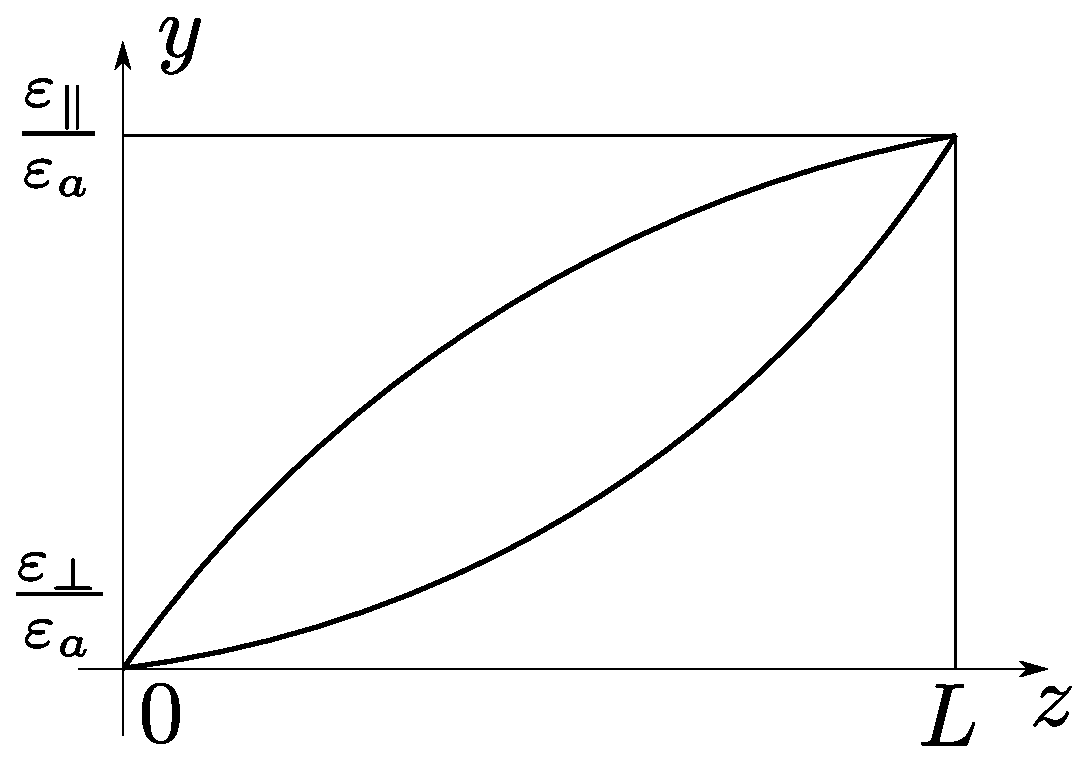
\includegraphics[width = 17pc]{ch5_profile_2.eps}
	\caption{Схематическое изображение параболических профилей без участков насыщения при $\mu_0 = \ve_\bot/\ve_a$ и $\mu_L = \ve_\|/\ve_a$.}\label{fig:ch5_profile_2}
\end{figure}
Проверим, при каких значениях напряжения $U$ выполнено условие на вершину параболы.
В данном случае может быть выполнено только первое условие из совокупности~\eqref{eq:ch5_parabolic_system_5}.
Подставляя в выражение для коэффициента $b$~\eqref{eq:ch5_parabolic_coeff_system_1} ``нижний'' знак при $\gamma$ и исследуемые значения $\mu_{0, L}$, запишем первое условие  из~\eqref{eq:ch5_parabolic_system_5}:
\begin{subequations}
	\begin{empheq}[left = \empheqlbrack]{align}
		&\frac{L}{2}\left( \frac{-\gamma}{\frac{\ve_\|}{\ve_\bot} - \gamma} + \frac{1}{1 - \gamma} \right) < 0,\label{eq:ch5_system_2_a}\\
		&\frac{L}{2}\left( \frac{-\gamma}{\frac{\ve_\|}{\ve_\bot} - \gamma} + \frac{1}{1 - \gamma} \right) > L.\label{eq:ch5_system_2_b}
	\end{empheq}
\end{subequations}
Рассмотрим неравенство~\eqref{eq:ch5_system_2_a}.
После несложных преобразований можно прийти к следующей записи:
\begin{equation}\label{eq:ch5_case_2_ineq_1}
	\frac{1}{1 - \gamma} < \frac{\gamma}{\frac{\ve_\|}{\ve_\bot} - \gamma}
\end{equation}
Заметим, что $\ve_\|/\ve_\bot > 1$ (так как рассматривается случай $\ve_a > 0$), а $\gamma < 1$.
Отсюда можно сделать вывод, что неравенство~\eqref{eq:ch5_case_2_ineq_1} не может быть выполнено.
Отсюда также следует, что профиль, обозначенный на Рис.~\ref{fig:ch5_profile_2} пунктирной линией, не может быть равновесным.

Рассмотрим неравенство~\eqref{eq:ch5_system_2_b}.
Его при помощи алгебраических преобразований можно свести к следующему виду:
\begin{equation}\label{eq:ch5_case_2_ineq_2}
	(1 - \gamma)^2 < (2\gamma -1)\frac{\ve_a}{\ve_\bot}.
\end{equation}
Графики функций $f_1(\gamma) = (1-\gamma)^2$ и $f_2(\gamma) = (2\gamma - 1)\ve_a/\ve_\bot$ представлены на Рис.~\ref{fig:ch5_graph_solver_2}.
\begin{figure}[h]
	\centering
	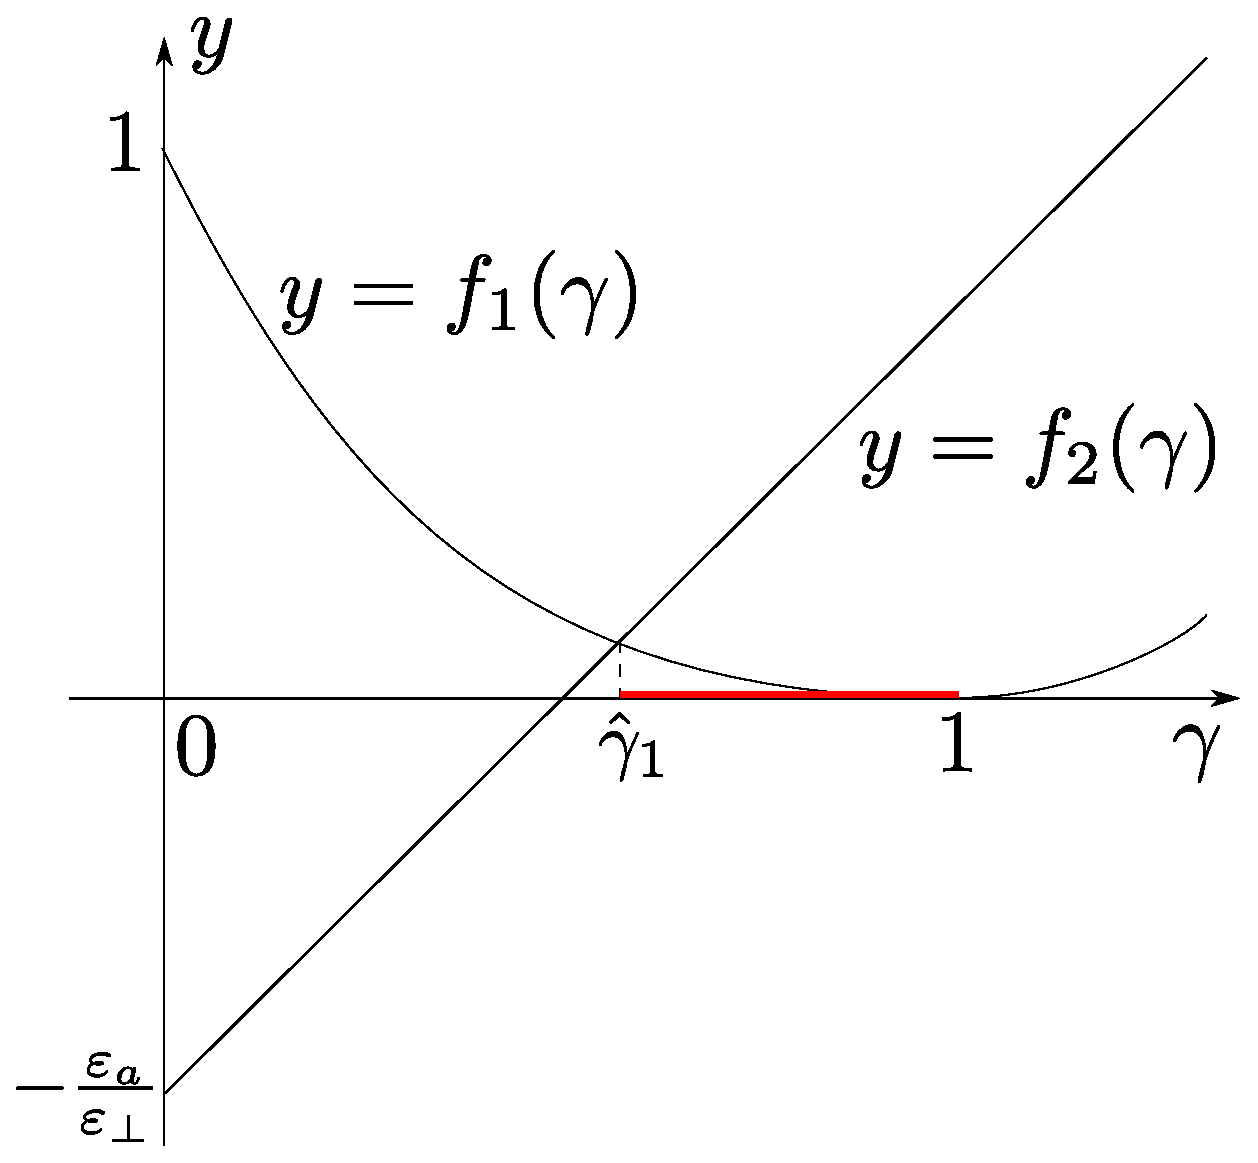
\includegraphics[width=20pc]{ch5_graph_solver_2.eps}
	\caption{Графики функций $y = f_1(\gamma)$ и $y = f_2(\gamma)$. Цветом выделен участок на оси $\gamma$, соответствующий решению неравенства~\eqref{eq:ch5_case_2_ineq_2}.}\label{fig:ch5_graph_solver_2}
\end{figure}
Здесь при построении графика учтено, как соотносятся значения обеих функций при $\gamma = 0$ и $\gamma = 1$.
Таким образом, неравенство~\eqref{eq:ch5_case_2_ineq_2} выполнено, когда $\gamma\in(\hat{\gamma}_1,\,1]$, что соответствует $U\in[0,\, \hat{U}_1)$.
Решая квадратное уравнение, можно получить точное выражение для $\hat{\gamma}_1$ и напряжения $\hat{U}_1$:
\begin{align}
	&\hat{\gamma}_1 = \frac{\ve_\|}{\ve_\bot} + \frac{\ve_\|}{\ve_\bot}\sqrt{\frac{\ve_a}{\ve_\|}},\\
	&\hat{U}_1 = \frac{8\pi \bar{e}}{\ve_a}\ln\left( \frac{1}{\hat{\gamma}_1} \right)
\end{align}
Вновь, условие $U > \tilde{U}$ отвечает за выполнение неравенства~\eqref{eq:ch5_right_border_ineq} на правой границе, а условие $U < \hat{U}_1$ порождено требованием на вершину параболы.

Таким образом, можно видеть, что при
\begin{equation}\label{eq:ch5_case_2_ineq_3}
\tilde{U} < U < \hat{U}_1
\end{equation}
равновесной будет ориентационная структура, профиль $y(z)$ которой обозначен на Рис.~\ref{fig:ch5_profile_2} сплошной линией.
Подставляя в~\eqref{eq:ch5_parabolic_system_1} выражения для коэффициентов~\eqref{eq:ch5_parabolic_coeff_system} с учётом $\mu_0 = \ve_\bot/\ve_a$, $\mu_L = \ve_\|/\ve_a$ и ``нижнего'' при $\gamma$, получим уравнение этого профиля в явном виде:
\begin{multline}\label{eq:ch5_asymmetric_parabolic_profile}
	y(z) = -\frac{\ve_\bot}{\ve_a}\cdot\frac{(1-\gamma)\left(\frac{\ve_\|}{\ve_\bot} - \gamma \right)}{\gamma}\left[ \frac{z}{L} - \frac{1}{2}\cdot\frac{(1 - \gamma)^2 + \frac{\ve_a}{\ve_\bot}}{(1 - \gamma)\left( \frac{\ve_\|}{\ve_\bot} - \gamma \right)} \right] +\\
	+ \frac{\ve_\bot}{\ve_a}\cdot\frac{\left( \frac{\ve_\|}{\ve_\bot} - \gamma^2 \right)^2}{\gamma(1-\gamma)\left( \frac{\ve_\|}{\ve_\bot} - \gamma \right)}.
\end{multline}

Заметим, что для того, чтобы интервал напряжений, задаваемый двойным неравенством~\eqref{eq:ch5_case_2_ineq_3}, был непустым, также необходимо, чтобы выполнялось следующее неравенство:
\begin{equation}
	\tilde{U} < \hat{U}_1
\end{equation}
Для дальнейшего анализа удобно ввести обозначение
\begin{equation}
	\varkappa = \sqrt{\frac{\ve_\|}{\ve_a}}
\end{equation}
и записать найденные выше характеристические напряжения $\tilde{U}$, $\hat{U}'$ и $\hat{U}_1$ с его помощью:
\begin{subequations}\label{eq:ch5_case_2_ineqs_4}
	\begin{align}
		&\tilde{U} = \frac{8\pi\bar{e}}{\ve_a}\ln\left( 1 + \frac{g_2 L}{2} \right),\\
		&\hat{U}' = \frac{8\pi\bar{e}}{\ve_a}\ln\frac{\varkappa + 1}{\varkappa - 1},\\
		&\hat{U}_1 = \frac{8\pi\bar{e}}{\ve_a}\ln\frac{\varkappa + 1}{\varkappa}.
	\end{align}
\end{subequations}
Отметим, что $\hat{U}_1 < \hat{U}'$.
Значит, остаётся три возможных варианта взаимного расположения напряжений:
\begin{subequations}
	\begin{align}
		&\hat{U}_1 < \hat{U}' < \tilde{U},\\
		&\hat{U}_1 < \tilde{U} < \hat{U}',\\
		&\tilde{U} < \hat{U}_1 < \hat{U}'.
	\end{align}
\end{subequations}
С учётом явно выраженный напряжений~\eqref{eq:ch5_case_2_ineqs_4} эти неравенства можно переписать следующим образом:
\begin{subequations}\label{eq:ch5_case_2_ineqs_5}
	\begin{align}
		&\frac{2}{\varkappa} < \frac{4}{\varkappa - 1} < g_2 L,\label{eq:ch5_case_2_ineqs_5_a}\\
		&\frac{2}{\varkappa} < g_2 L < \frac{4}{\varkappa - 1},\label{eq:ch5_case_2_ineqs_5_b}\\
		&g_2 L < \frac{2}{\varkappa} < \frac{4}{\varkappa - 1}.\label{eq:ch5_case_2_ineqs_5_c}
	\end{align}
\end{subequations}
Видно, что параметром, который отвечает за то, какой сценарий будет реализован в данной системе (при данном наборе параметров), является $g_2 L$.
Выясним, каким именно сценариям трансформации ориентационной структуры с изменнением $U$ соответствуют ситуации~\eqref{eq:ch5_case_2_ineqs_5}.
\begin{itemize}
	\item Случай ``сильного'' сцепления, $2/\varkappa < g_2 L$.
	
	При таких значениях параметра $g_2 L$ будет реализован сценарий, схематически изображённый на Рис.~\ref{fig:ch5_scheme_nonsaturated_part_1}.
	\begin{figure}[h]
		\centering
		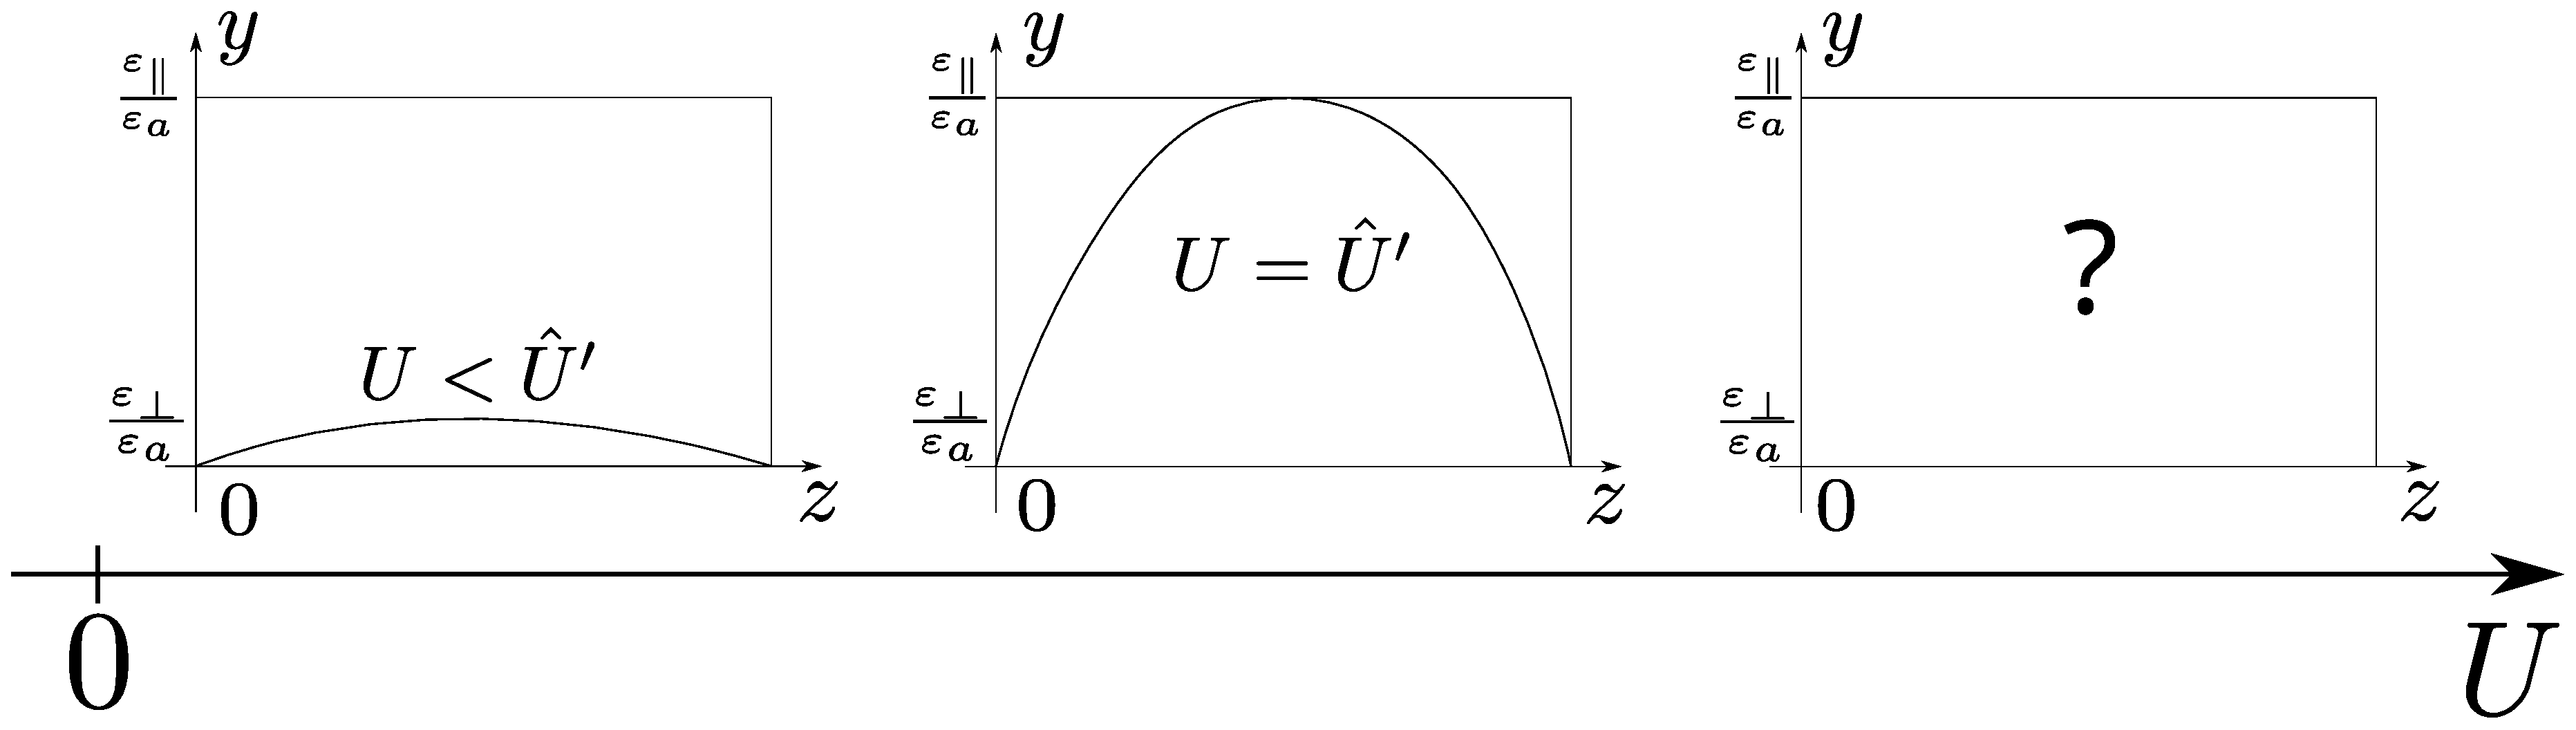
\includegraphics[width=\textwidth]{ch5_scheme_nonsaturated_part_1.eps}
		\caption{Схематическое изображение трансформации профилей $y(z)$ с ростом приложенного напряжения $U$ в случае ``сильного'' сцепления, задаваемого неравенством~\eqref{eq:ch5_case_2_ineqs_5_a}.}\label{fig:ch5_scheme_nonsaturated_part_1}
	\end{figure}
	Видно, что с ростом $U$ от $U = 0$ сначала происходит небольшое искажение структуры вблизи середины ячейки, затем это искажение распространяется ближе к границам и становится всё сильнее.
	При этом ориентация на обеих границах остаётся планарной.
	Наконец, профиль $y(z)$ касается ``верхней границы'' в середине ячейки при $U = \hat{U}'$.
	Дальнейшая эволюция ориентационной структуры ЖК требует рассмотрения профилей с участками насыщения, что будет проделано в части~\ref{sec:sec5.1}.
	На данном этапе эти стадии эволюции отмечены знаками вопроса.
	Отметим, что здесь и на остальных аналогичных схемах по оси напряжений отсутствует масштаб, она нанесена, чтобы показать, в каком порядке сменяются профили с ростом $U$.
	Кроме того, можно увидеть, что в данном сценарии не упоминается напряжение $\hat{U}_1$.
	Это происходит из-за того, что оно соответствует нарушению условия на вершину параболы для асимметричного профиля без участков насыщения, который в данном случае не может быть равновесным.

	\item Случай ``среднего'' сцепления, $4/(\varkappa - 1) < g_2 L < 2/\varkappa$.
	
	При данных значениях параметра $g_2 L$, характеризующего сцепление с подложкой, реализуется сценарий, схематиччески изображённый на Рис.~\ref{fig:ch5_scheme_nonsaturated_part_2}.
	\begin{figure}[h]
		\centering
		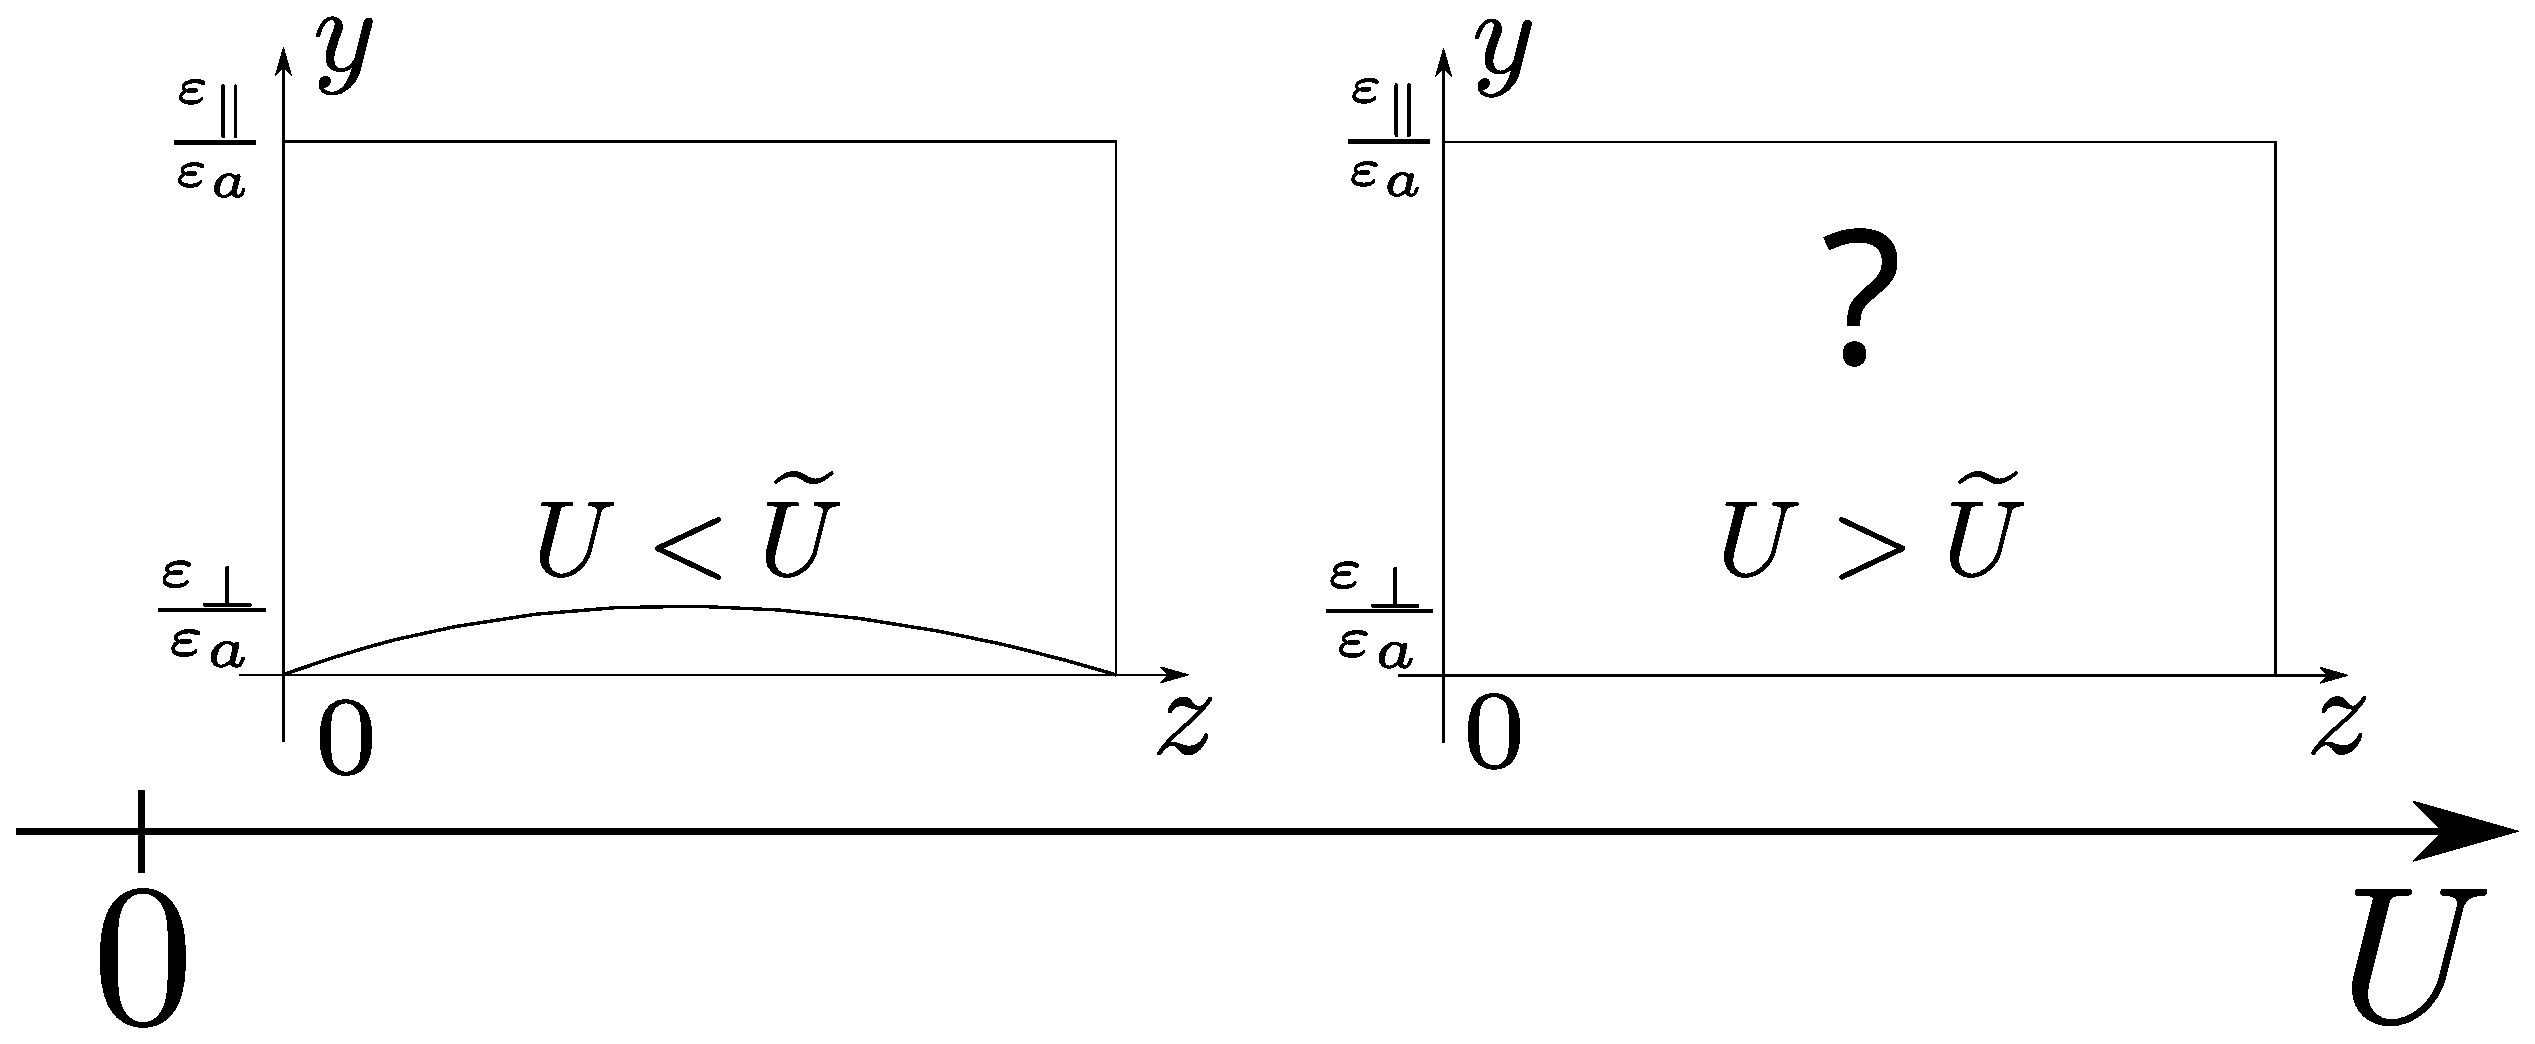
\includegraphics[width=0.7\textwidth]{ch5_scheme_nonsaturated_part_2.eps}
		\caption{Схематическое изображение трансформации профилей $y(z)$ с ростом приложенного напряжения $U$ в случае ``среднего'' сцепления, задаваемого неравенством~\eqref{eq:ch5_case_2_ineqs_5_b}.}\label{fig:ch5_scheme_nonsaturated_part_2}
	\end{figure}
	В этом случае единственным возможным решением без участков насыщения является профиль, задаваемый уравнением~\eqref{eq:ch5_simple_parabolic_profile}.
	Это происходит из-за того, что симметричный (относительно $z = L/2$) параболический профиль является равновесным, пока выполнено неравенство
	\begin{equation}
		U < \min(\tilde{U}, \hat{U}'),
	\end{equation}
	которое в данном случае сводится к $U < \tilde{U}$.
	Поясним, почему в данном случае при рассмотрении изменения ориентационной структуры с ростом $U$ мы не упоминаем напряжения $\hat{U}_1$ и $\hat{U}'$.
	Напряжение $\hat{U}'$ отвечает за касание вершиной симметричного параболического профиля верхней границы, $\ve_\|/\ve_a$ (эта ситуация изображена на второй диаграмме на Рис.~\ref{fig:ch5_scheme_nonsaturated_part_2}), однако этого произойти не может, так как сначала будет достигнуто напряжение $\tilde{U}$, и условие на правой границе~\eqref{eq:ch5_parabolic_system_7} нарушится для симметричного профиля.
	В свою очередь, напряжение $\hat{U}_1$ разделяет случаи, когда вершина асимметричного профиля располагается вне ($U < \hat{U}_1$) или внутри ($U > \hat{U}_1$, такой профиль уже не физичен) интервала $(0,\,L)$.
	Однако при переходе через $\tilde{U}$ и потере устойчивости на правой границе оказывается, что $U > \hat{U}_1$, а значит, асимметричный профиль без участка насыщения не возникает.
	
	\item Случай ``слабого'' сцепления, $g_2 L < 4/(\varkappa - 1)$.
	
	Наконец, при даных значениях параметра $g_2 L$ 
	\begin{figure}[h]
		\centering
		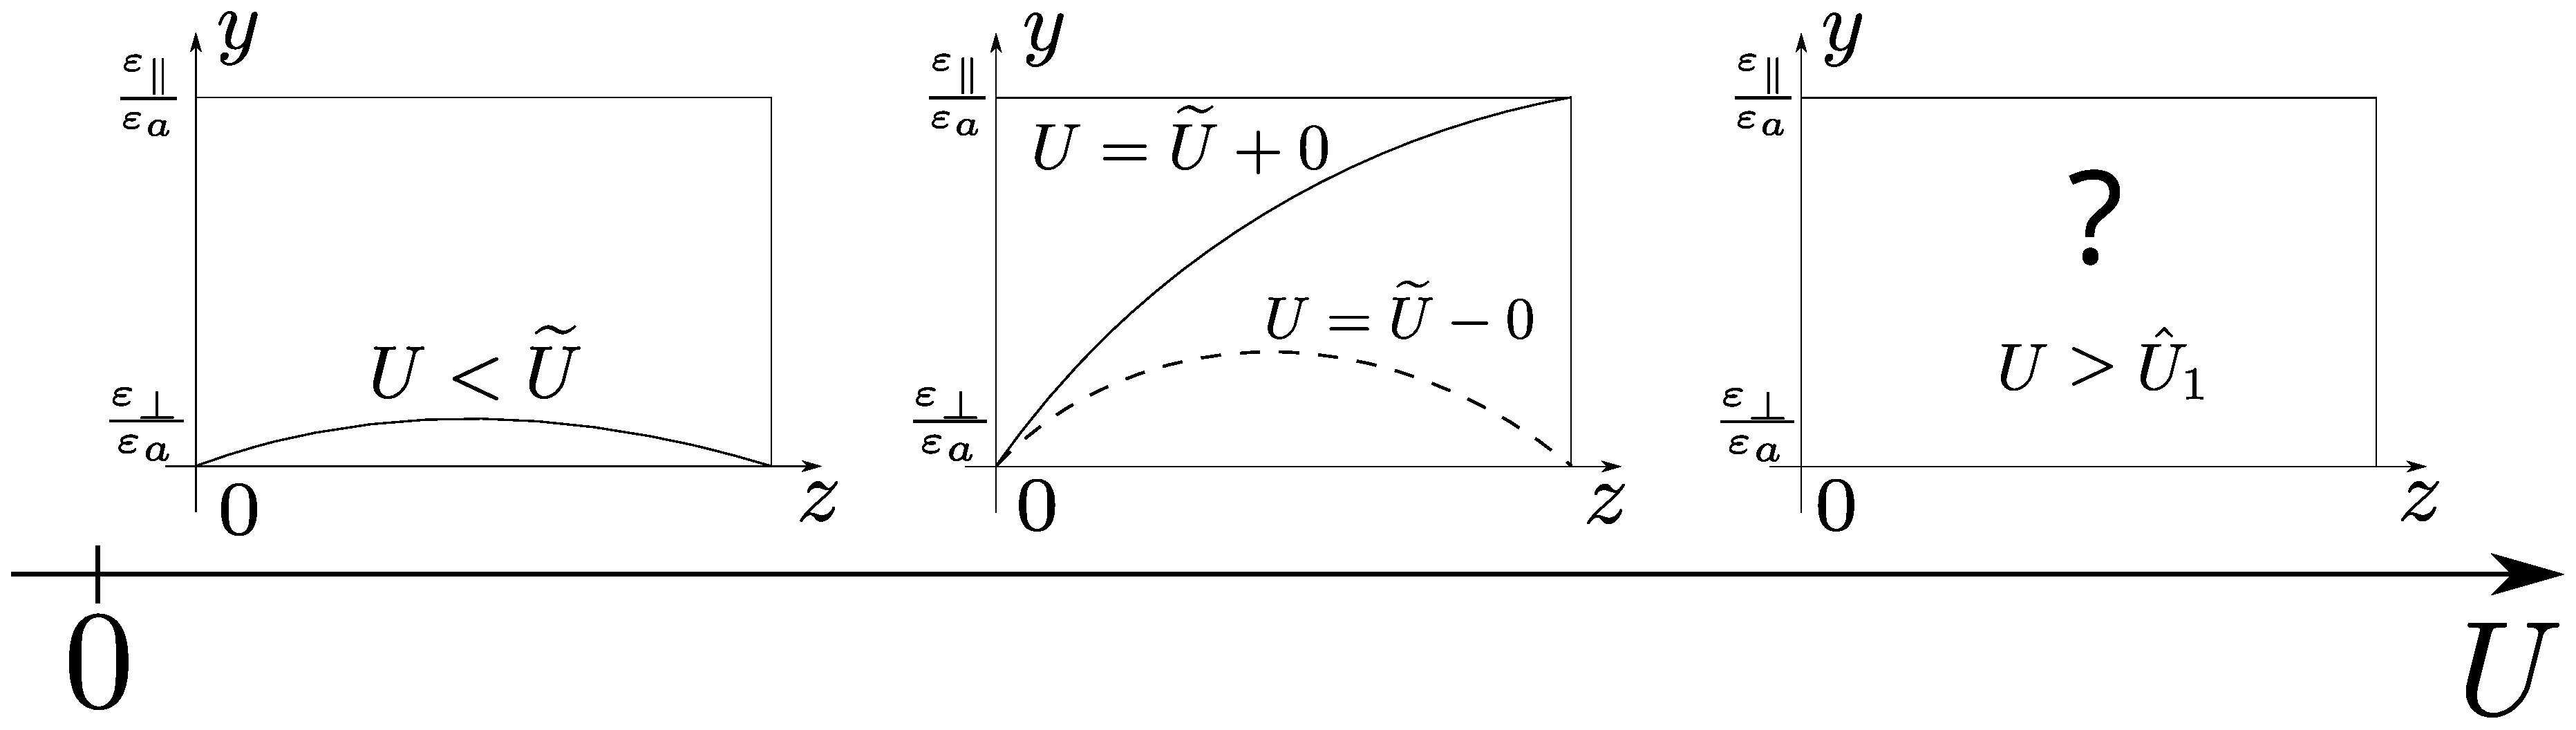
\includegraphics[width=\textwidth]{ch5_scheme_nonsaturated_part_3.eps}
		\caption{Схематическое изображение трансформации профилей $y(z)$ с ростом приложенного напряжения $U$ в случае ``слабого'' сцепления, задаваемого неравенством~\eqref{eq:ch5_case_2_ineqs_5_c}.}\label{fig:ch5_scheme_nonsaturated_part_3}
	\end{figure}
	Здесь симметричный параболический профиль остаётся равновесным, пока напряжение $U$ не превысит значения $\tilde{U}$, после чего равновесным становится параболический профиль с разными значениями на границах, задаваемый уравнением~\eqref{eq:ch5_asymmetric_parabolic_profile}.
	В свою очередь, асимметричный профиль без участков насыщения остаётся равновесным до достижения следующего порогового напряжения, $\hat{U}_1$, после чего равновесным будет уже профиль с участками насыщения.
	В данном случае оказалось неупомянутым напряжение $\hat{U}'$, так как симметричный профиль теряет устойчивость на правой границе ещё до того, как его вершина коснётся границы $y = \ve_\|/\ve_a$.
\end{itemize}

\section{Решения с участком насыщения}

Рассмотрим решения с единственным участком насыщения.
Расчёт равновесных профилей при помощи прямой минимизации свободной энергии проказал, что при $\ve_a, U > 0$ возникают профили только трёх типов.
Они схематически изображены на Рис.~\ref{fig:ch5_profiles_saturated}.
\begin{figure}
	\begin{minipage}{0.32\textwidth}
		\centering
		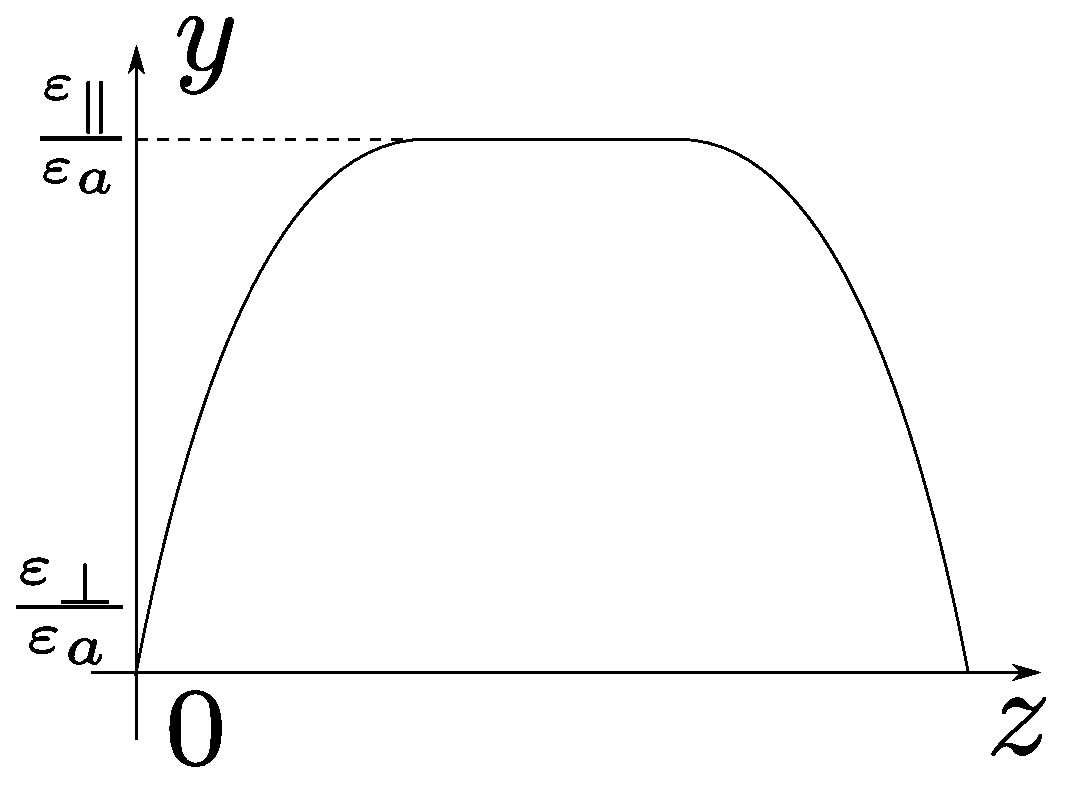
\includegraphics[width=\textwidth]{ch5_profiles_saturated_a.eps}
		{А}
	\end{minipage}
	\hfill
	\begin{minipage}{0.32\textwidth}
		\centering
		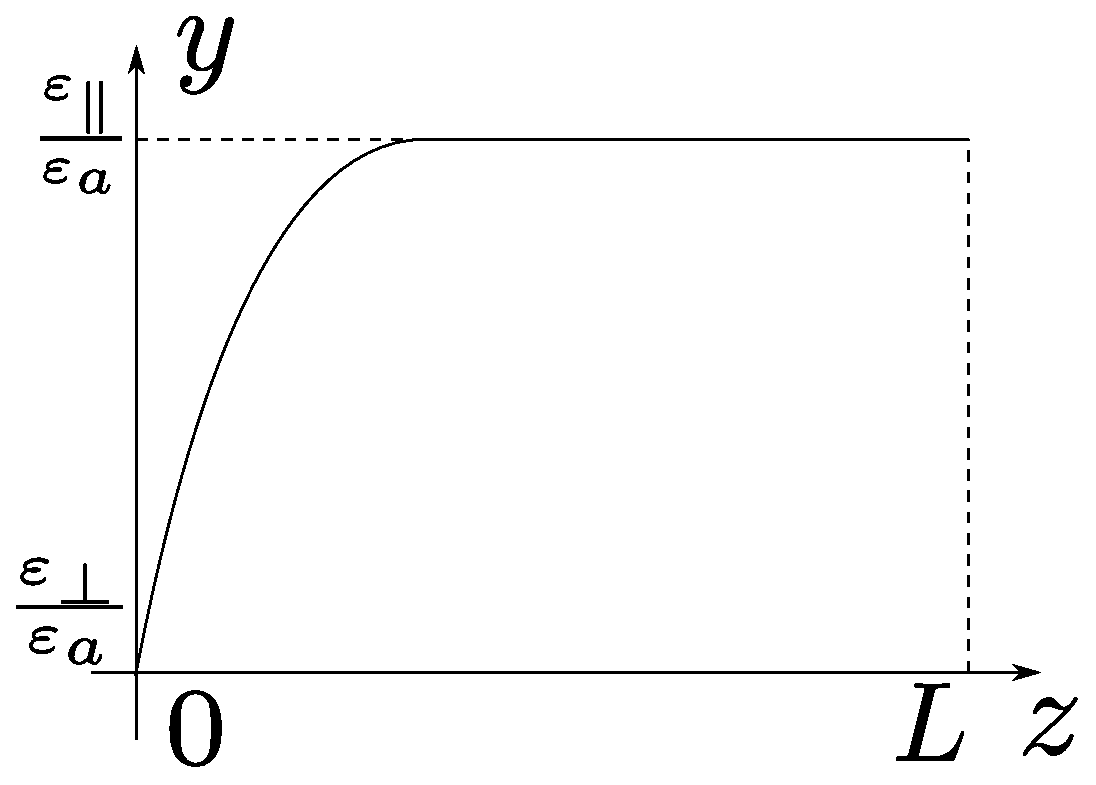
\includegraphics[width=\textwidth]{ch5_profiles_saturated_b.eps}
		{Б}
	\end{minipage}
	\hfill
	\begin{minipage}{0.32\textwidth}
		\centering
		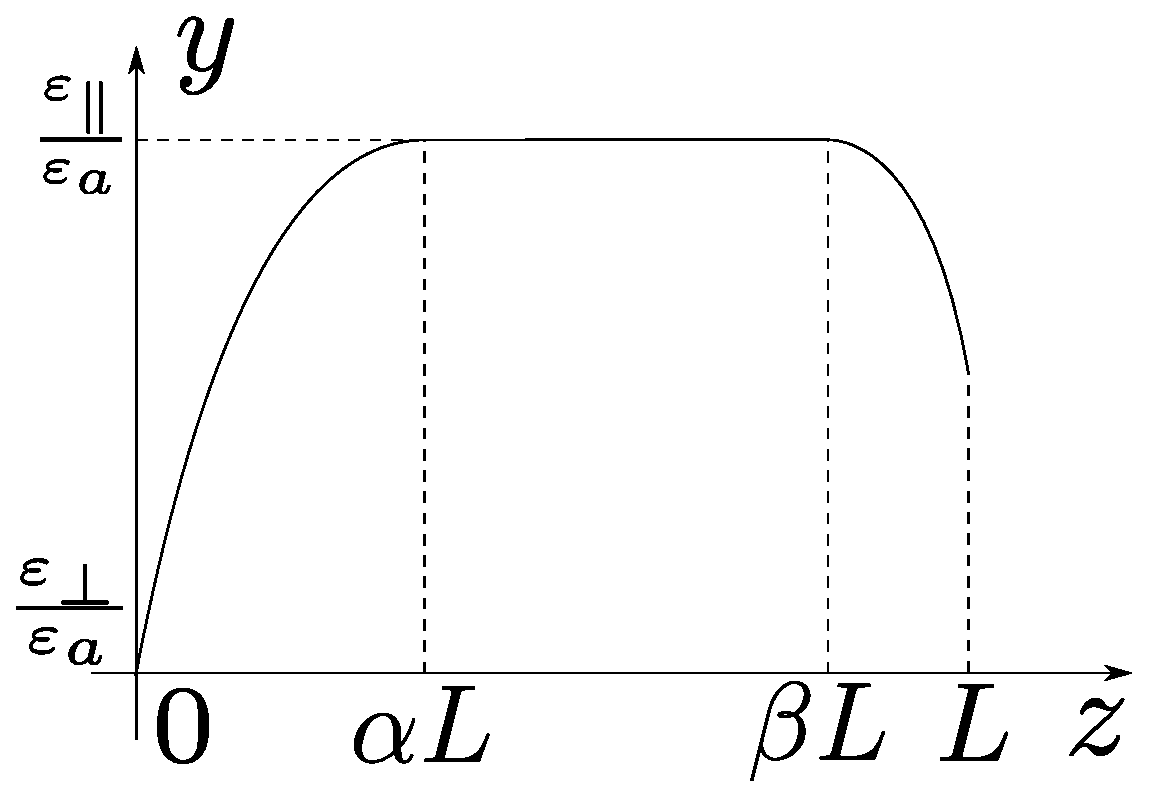
\includegraphics[width=\textwidth]{ch5_profiles_saturated_c.eps}
		{В}
	\end{minipage}
	\vspace{0.5cm}
	\caption{Схематическое изображение различных видов профилей с участками насыщения, полученных при помощи численной минимизации свободной энергии.}
	\label{fig:ch5_profiles_saturated}
\end{figure}
Перед тем, как мы начнём получать их уравнения, отметим следующую особенность: в данном случае искомая функция $y(z)$ состоит из нескольких частей.
При этом на каждую точку сшивания $z_0$ добавляется ещё по два условия: на функцию, $y(z_0 - 0) = y(z_0 + 0)$, и на производную, $y'(z_0 - 0) = y'(z_0 + 0)$.

\paragraph{Случай А. Симметричный профиль с участком насыщения.}
Будем искать решение следующего вида:
\begin{equation}
	y(z) = 
	\begin{cases}
		y_1(z),\quad z\in [0,\,\alpha L],\\
		\frac{\ve_\|}{\ve_a},\quad z\in (\alpha L,\, \beta L),\\
		y_3(z),\quad z\in [\beta L,\,L].
	\end{cases}
\end{equation}
Отметим, что и $y_1$, и $y_3$ должны решать одно и то же уравнение~\eqref{eq:parametric_EL}, а значит, обе они имеют вид~\eqref{eq:parabolic_solution} с общим коэффициентом $a$ и отличаясь только коэффициентами $b$ и $c$ ($b_1$, $c_1$ и $b_3$ и $c_3$ соответственно).
Запишем ``геометрические'' условия на функцию $y_1(z)$:
\begin{subequations}\label{eq:ch5_saturated_case_a_system_1}
	\begin{empheq}[left = \empheqlbrace]{align}
		&y_1(z) = \frac{c_1}{4}(z + b_1)^2 - \frac{a^2}{c_1},\label{eq:ch5_saturated_case_a_system_1_1}\\
		&y_1(0) = \frac{\ve_\bot}{\ve_a},\label{eq:ch5_saturated_case_a_system_2}\\
		&y_1(\alpha L) = \frac{\ve_\|}{\ve_a},\label{eq:ch5_saturated_case_a_system_3}\\
		&y_1'(\alpha L) = 0.\label{eq:ch5_saturated_case_a_system_4}
	\end{empheq}
\end{subequations}
Нетрудно видеть, что требование сшивания производных может быть выполнено тогда и только тогда, когда вершина параболы $y_1(z)$ находится в точке с координатами $(\alpha L,\, \ve_\|/\ve_a)$, а значит, $b_1 = -\alpha L$.
Подстановка~\eqref{eq:ch5_saturated_case_a_system_1} в~\eqref{eq:ch5_saturated_case_a_system_2} и~\eqref{eq:ch5_saturated_case_a_system_3} приводит к следующему виду $y_1(z)$:
\begin{equation}\label{eq:ch5_saturated_case_a_eq_3}
	y_1(z) = -\left( \frac{z}{\alpha L} - 1 \right)^2 + \frac{\ve_\|}{\ve_a}.
\end{equation}
Аналогичные рассуждения можно провести и для $y_3(z)$.
Отметим, что условия $y_1(0) = y_3(L)$ и $y_1(\alpha L) = y_3(\beta L)$ приводят к тому, что параболы $y_1(z)$ и $y_3(z)$ оказываются симметричными относительно $z = L/2$.
Это означает, в частности, что $\alpha = 1 - \beta$.
Таким образом, для $y_3(z)$ имеем:
\begin{equation}
y_3(z) = -\left( \frac{z}{\alpha L} - \frac{1}{\alpha} + 1 \right)^2 + \frac{\ve_\|}{\ve_a}.
\end{equation}
Кроме того, из этих же условий можно получить следующе выражение для $a$:
\begin{equation}\label{eq:ch5_saturated_case_a_eq_1}
	a = -\frac{2\varkappa}{\alpha L}.
\end{equation}
Для того, чтобы определить значение параметра $\alpha$, следует подставить полученную зависимость $y(z)$ в условие самосогласования~\eqref{eq:parameter_a}:
\begin{equation}\label{eq:ch5_saturated_case_a_eq_2}
	a\frac{(1 - 2\alpha)L}{2\varkappa^2} = \ln\left( \gamma \frac{\varkappa + 1}{\varkappa - 1} \right).
\end{equation}
Подставляя~\eqref{eq:ch5_saturated_case_a_eq_1} в~\eqref{eq:ch5_saturated_case_a_eq_2}, можно получить окончательное выражение для $1/\alpha$:
\begin{equation}
	\frac{1}{\alpha} = 2 - \varkappa\ln\left( \gamma\frac{\varkappa + 1}{\varkappa - 1} \right).
\end{equation}
Учитывая, что $\alpha$ ограниченa:
\begin{equation}
	0 < \alpha \leq \frac{1}{2},
\end{equation}
можно заметить, что в данном случае существует ограничение на $\gamma$:
\begin{equation}
	\gamma < \frac{\varkappa - 1}{\varkappa + 1}.
\end{equation}
Это эквивалентно условию $U > \hat{U}'$, где $\hat{U}'$ -- найденное в предыдущей части напряжение, при котором симметричный параболический профиль касается верхней границы (см. Рис.~\ref{fig:ch5_scheme_nonsaturated_part_1}).

Остаётся проверить, что выполнены граничные условия~\eqref{eq:ch5_parabolic_system_6} и~\eqref{eq:ch5_parabolic_system_7}.
Подстановка $y_1(z)$ в первое из них даёт
\begin{equation}
	g_1(\varkappa - 1)(\varkappa + 1) > \frac{2}{\alpha L}(1 - \varkappa),
\end{equation}
что верно всегда, поскольку $\varkappa > 1$.
Подстановка $y_3(z)$ во второе условие приводит к неравенству
\begin{equation}
	g_2 L > \frac{2}{\alpha(\varkappa - 1)}.
\end{equation}
Его можно интерпретировать следующим образом: так как $\alpha = \alpha(U)$, причём с ростом напряжения $\alpha$ монотонно уменьшается, то будет существовать некоторое критическое значение напряжения $\tilde{U}'$, при котором неравенство обратится в равенство, и при превышении которого исследуемый профиль перестанет быть равновесным.
Можно выписать явное выражение для этого порогового напряжения:
\begin{equation}
	\tilde{U}' = \hat{U}' + \frac{8\pi\bar{e}}{\ve_a}\left( \frac{g_2 L}{2}\cdot\frac{\varkappa - 1}{\varkappa} - \frac{2}{\varkappa} \right)
\end{equation}

Таким образом, симметричный профиль с участком насыщения является равновесным, когда выполнены два условия на напряжение, $\hat{U}' < U < \tilde{U}'$, причём указанный интервал напряжений непустой тогда и только тогда, когда $g_2L > 4/(\varkappa - 1)$.

\todo{Может, стоит привести итоговый вид функции $y(z)$ в виде кусочно-заданной функции?}

\paragraph{Асимметричный профиль с насыщеной правой границей.}
Рассмотрим профиль, схематически изображённый на Рис.~\ref{fig:ch5_profiles_saturated}\,Б.
Будем искать решение вида
\begin{equation}\label{eq:ch5_saturated_case_b_start}
y(z) = 
\begin{cases}
y_1(z),\quad z\in [0,\,\alpha L],\\
\frac{\ve_\|}{\ve_a},\quad z\in (\alpha L,\, L].
\end{cases}
\end{equation}
В данном случае необходимо найти единственную функцию $y_1(z)$, удовлетворяющую тем же условиям, что и одноимённая функция, найденная выше (система уравнений~\eqref{eq:ch5_saturated_case_a_system_1}); эти условия приводят к виду $y_1(z)$, повторяющему формулу~\eqref{eq:ch5_saturated_case_a_eq_3}:
\begin{equation}\label{eq:ch5_saturated_case_b_eq_1}
	y_1(z) = -\left( \frac{z}{\alpha L} - 1 \right)^2 + \frac{\ve_\|}{\ve_a}.
\end{equation}
Опять же, из этих условий можно получить выражение для $a$:
\begin{equation}\label{eq:ch5_saturated_case_b_eq_2}
	a = -\frac{2\varkappa}{\alpha L}.
\end{equation}
Подставляя~\eqref{eq:ch5_saturated_case_b_eq_1} в условие самосогласования~\eqref{eq:parameter_a}, получаем ещё одно уравнение:
\begin{equation}\label{eq:ch5_saturated_case_b_eq_3}
	a\frac{(1 - \alpha)L}{2\varkappa^2} = \ln\left( \gamma \frac{\varkappa + 1}{\varkappa} \right).
\end{equation}
Совмещая~\eqref{eq:ch5_saturated_case_b_eq_2} и~\eqref{eq:ch5_saturated_case_b_eq_3}, получаем выражение для $\alpha$:
\begin{equation}\label{eq:ch5_saturated_case_b_eq_4}
	\alpha = \left( 1 - \varkappa\ln\left( \gamma \frac{\varkappa + 1}{\varkappa} \right)\right)^{-1}.
\end{equation}
В данном случае мы также имеем ограничение на $\alpha$:
\begin{equation}
	0 < \alpha \leq 1.
\end{equation}
Видно, что это условие выполнено при $U > \hat{U}_1$, где $\hat{U}_1$ определено выражением~\eqref{eq:ch5_case_2_ineqs_5_c}.

Наконец, проверим, когда выполняется условия на границах.
подстановка $y_1(z)$ в~\eqref{eq:ch5_parabolic_system_6} приводит к тому же выражению, что было получено при рассмотрении предыдущего случая, а значит, и вывод совпадает: условие на границе $z = 0$ выполнено всегда.
Далее, подставляя~\eqref{eq:ch5_saturated_case_b_start} в~\eqref{eq:ch5_parabolic_system_7}, получаем неравенство:
\begin{equation}\label{eq:ch5_saturated_case_b_eq_5}
	g_2 \varkappa^2 + a \leq 0,
\end{equation}
откуда, с учётом~\eqref{eq:ch5_saturated_case_b_eq_2} и~\eqref{eq:ch5_saturated_case_b_eq_4}, можно получить, что существует критическое напряжение $\hat{U}_2$ такое, что при $U > \hat{U}_2$ условие~\eqref{eq:ch5_saturated_case_b_eq_4} будет выполнено.
Приведём явный вид выражения для $\hat{U}_2$:
\todo{
\begin{equation}
	\hat{U}_2 = \hat{U}_1 + \frac{8\pi\bar{e}}{\ve_a}\cdot\frac{1}{\varkappa}\left( \frac{g_2 L}{2} - 1\right)
\end{equation}
}
Отметим, что при рассмотрении данного вида профилей не возникает условия на $g_2 L$, а значит, такой профиль возникает в системе с любым значением $g_2 L$ при достаточно большом напряжении ($U > \hat{U}_2$).


\paragraph{Асимметричный профиль с ненасыщеной правой границей.}
Рассмотрим профиль, схематически изображённый на Рис.~\ref{fig:ch5_profiles_saturated}\,В.




\section{Сравнение аналитических результатов с расчётными}
В заключение приведём сравнение профилей, рассчитанных при помощи полной модели свободной энергии (\todo{x.xx}) и профилей, полученных аналитически нна основе анализа сокращённой модели свободной энергии (\todo{y.yy}).

\todo{Далее -- под переделку, выше -- переписанное.}

Можно заметить, что граничные условия~\eqref{boundary1} и~\eqref{boundary2} могут быть удовлетворены только когда
\begin{align}
&y(0) = \mu_0, \quad\; \mu_0=\ve_\bot/\ve_a \; \text{или} \;  \mu_0=\ve_\|/\ve_a,  \label{y_mu0}\\  
&y(L) = \mu_L, \quad \mu_L=\ve_\bot/\ve_a \; \text{или} \;  \mu_L=\ve_\| /\ve_a, \label{y_muL}
\end{align}
то есть граничные условия могут быть легко проверены путём определения знака выражения, стоящего в квадратных скобках.
\todo{Каких скобках? Непонятно.}
\todo{АО: В статье говорится, что точные выражения для параметров сложные, а здесь нужно привести.}

\todo{Не для иллюстрации, это сама по себе цель.}
Для того, чтобы проиллюстрировать полученные результаты, мы аналитически и численно рассчитали зависимости $y(z)$ и $\theta(z)$.
В дальнейшем ограничимся рассмотрением случая положительно анизотропии диэлектрической проницаемости, $\ve_a > 0$.
Методика поиска равновесной ориентационной структуры ЖК в ячейке путём численной минимизации функционала свободной энергии аналогична таковой, применённой в предыдущих главах.
При этом был использован следующий набор параметров системы: $L = 0.006$~см, $\ve_\bot = 7.2$, $\ve_\|  = 16.2$, $\ve_a = 9$, $\bar{e} = 0.01$~Фр/см.
Было обнаружено, что, в зависимости от значения $g_2 L$, трансформация ориентационной структуры с изменением приложенного напряжения $U$ может происходить по трём различным сценариям.
На Рис.~\ref{ch5:fig1} показана трансформация ориентационной структуры при достаточно небольшой энергии сцепления с правой подложкой $W_\theta^{(2)}$, когда выполнено следующее неравенство:
\begin{equation}\label{ineq_g2L_1}
g_2 L < \frac{2}{\varkappa},
\end{equation}
где $\varkappa = \sqrt{\ve_\| /\ve_a}$.
\begin{figure}[h]
	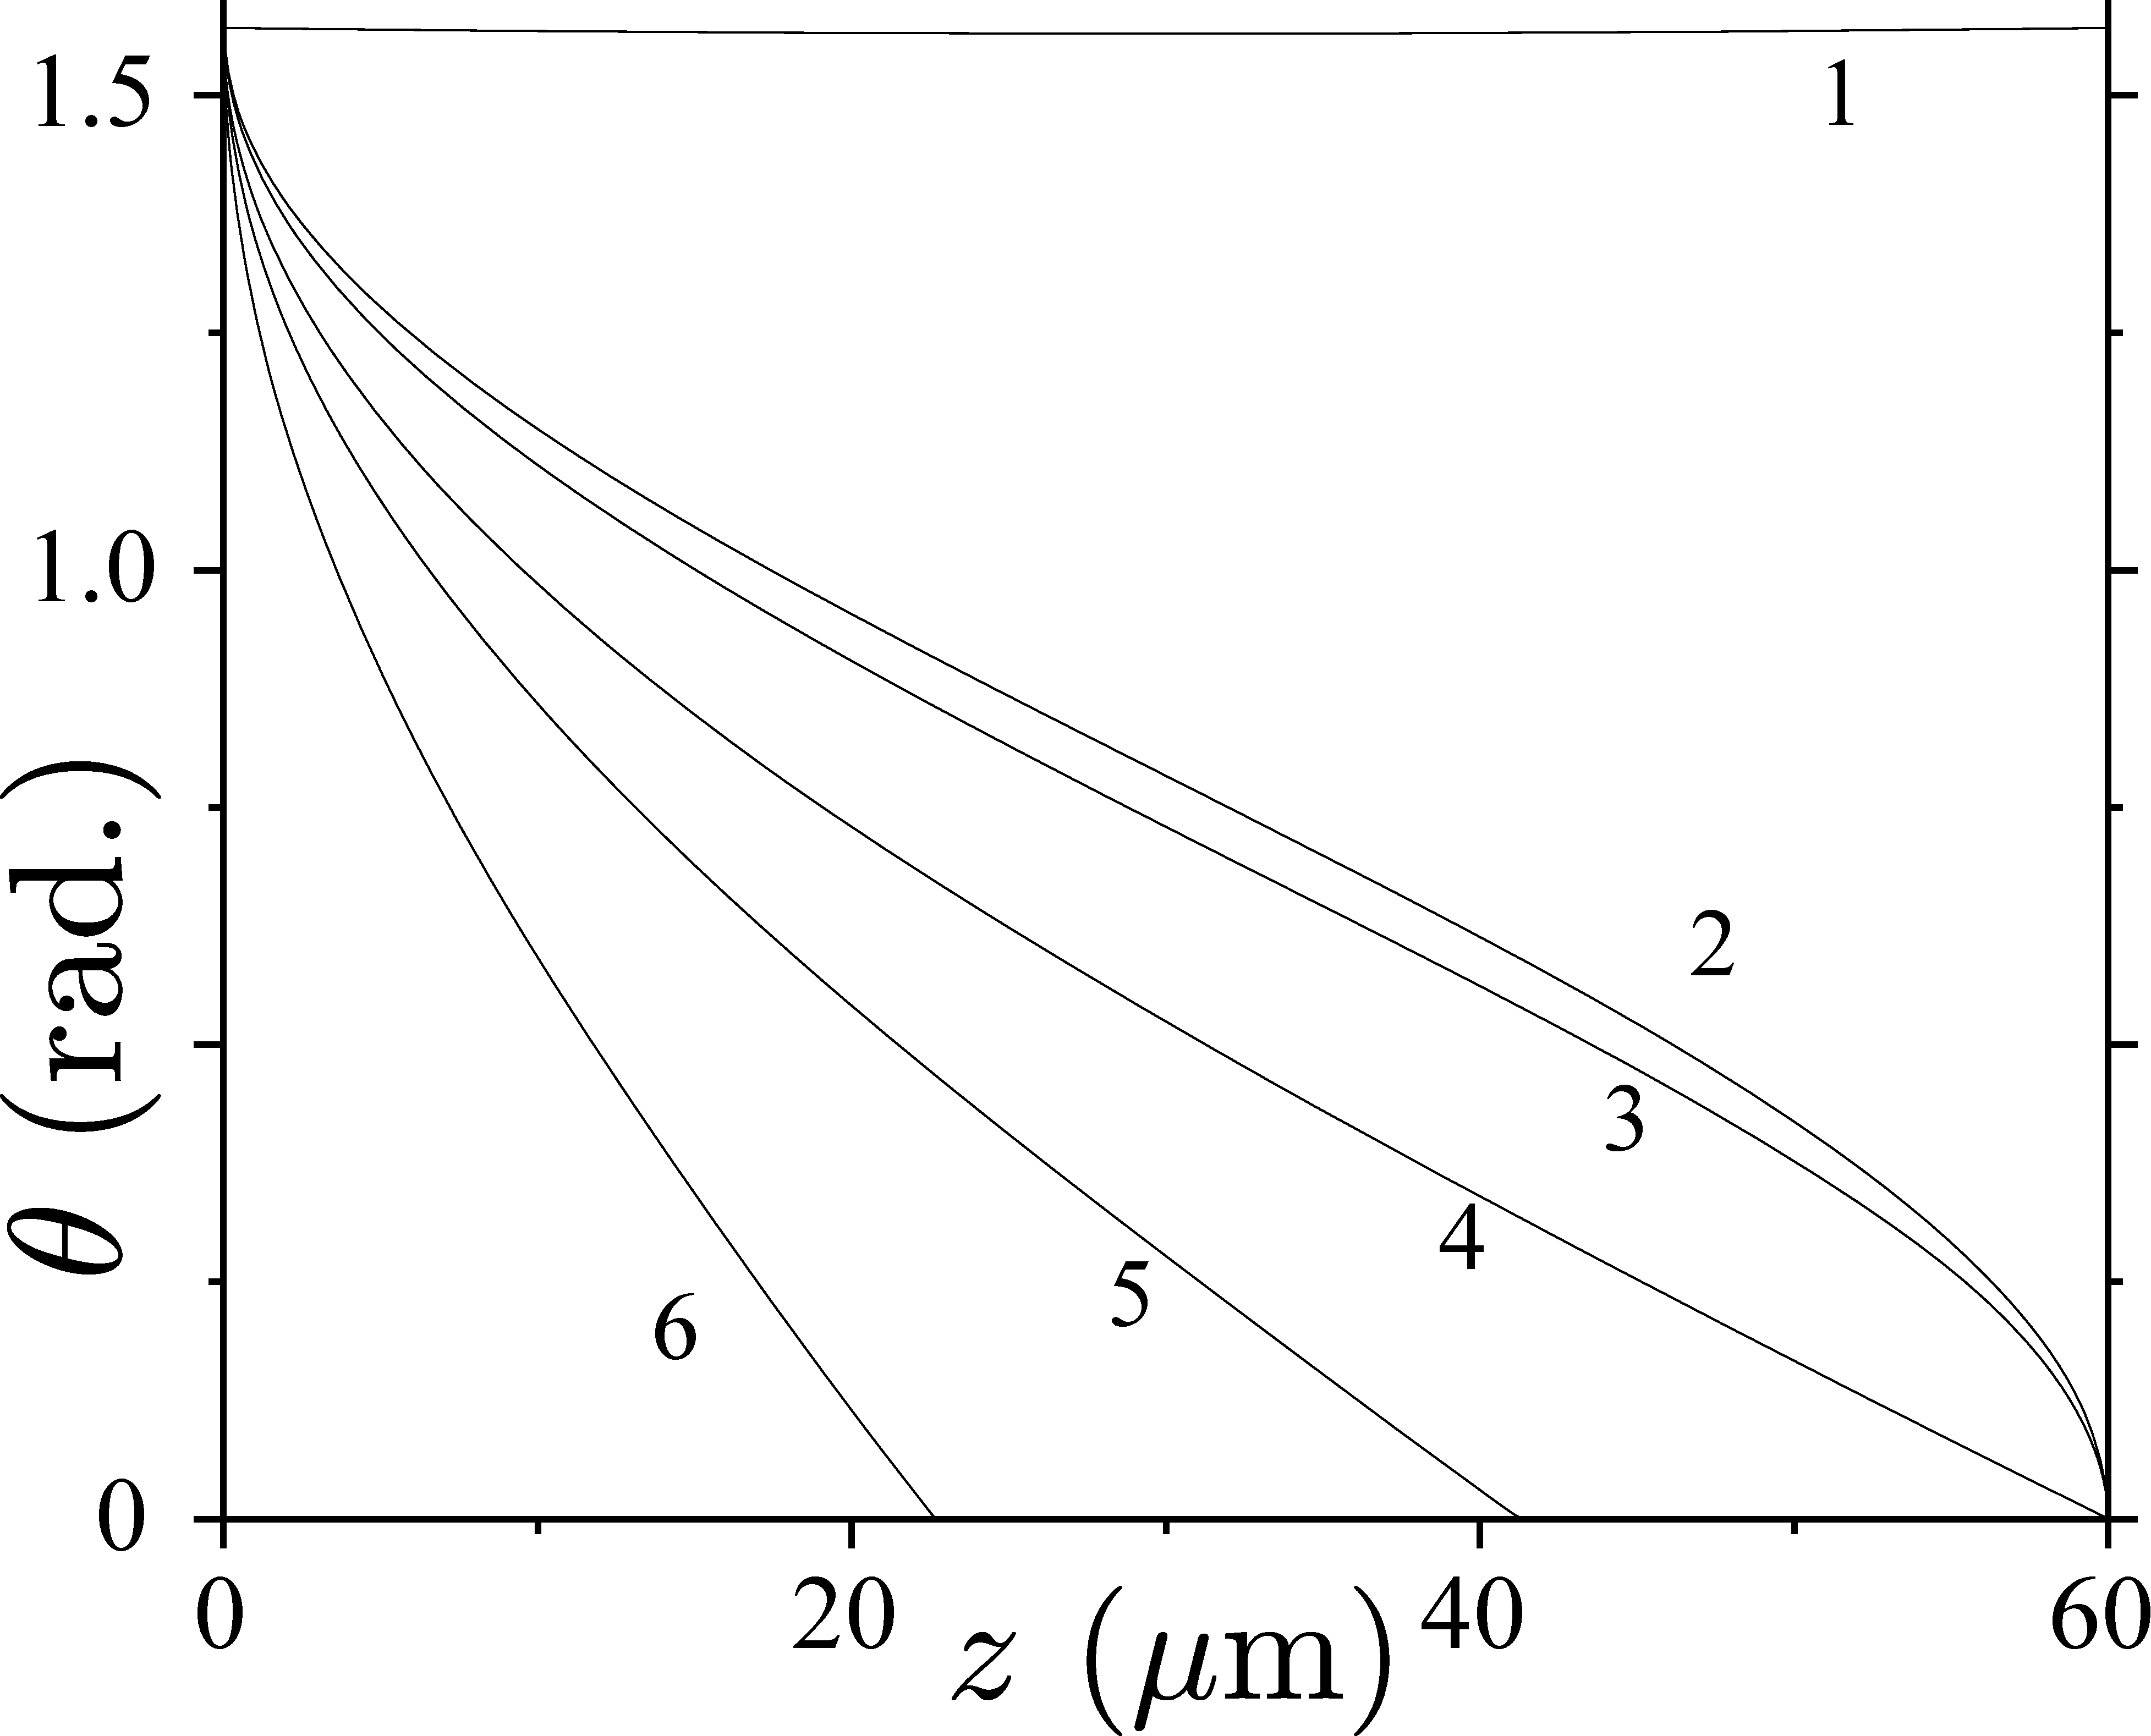
\includegraphics[width=17pc]{Fig1_theta_low_anchoring.eps}\hspace{2pc}%
	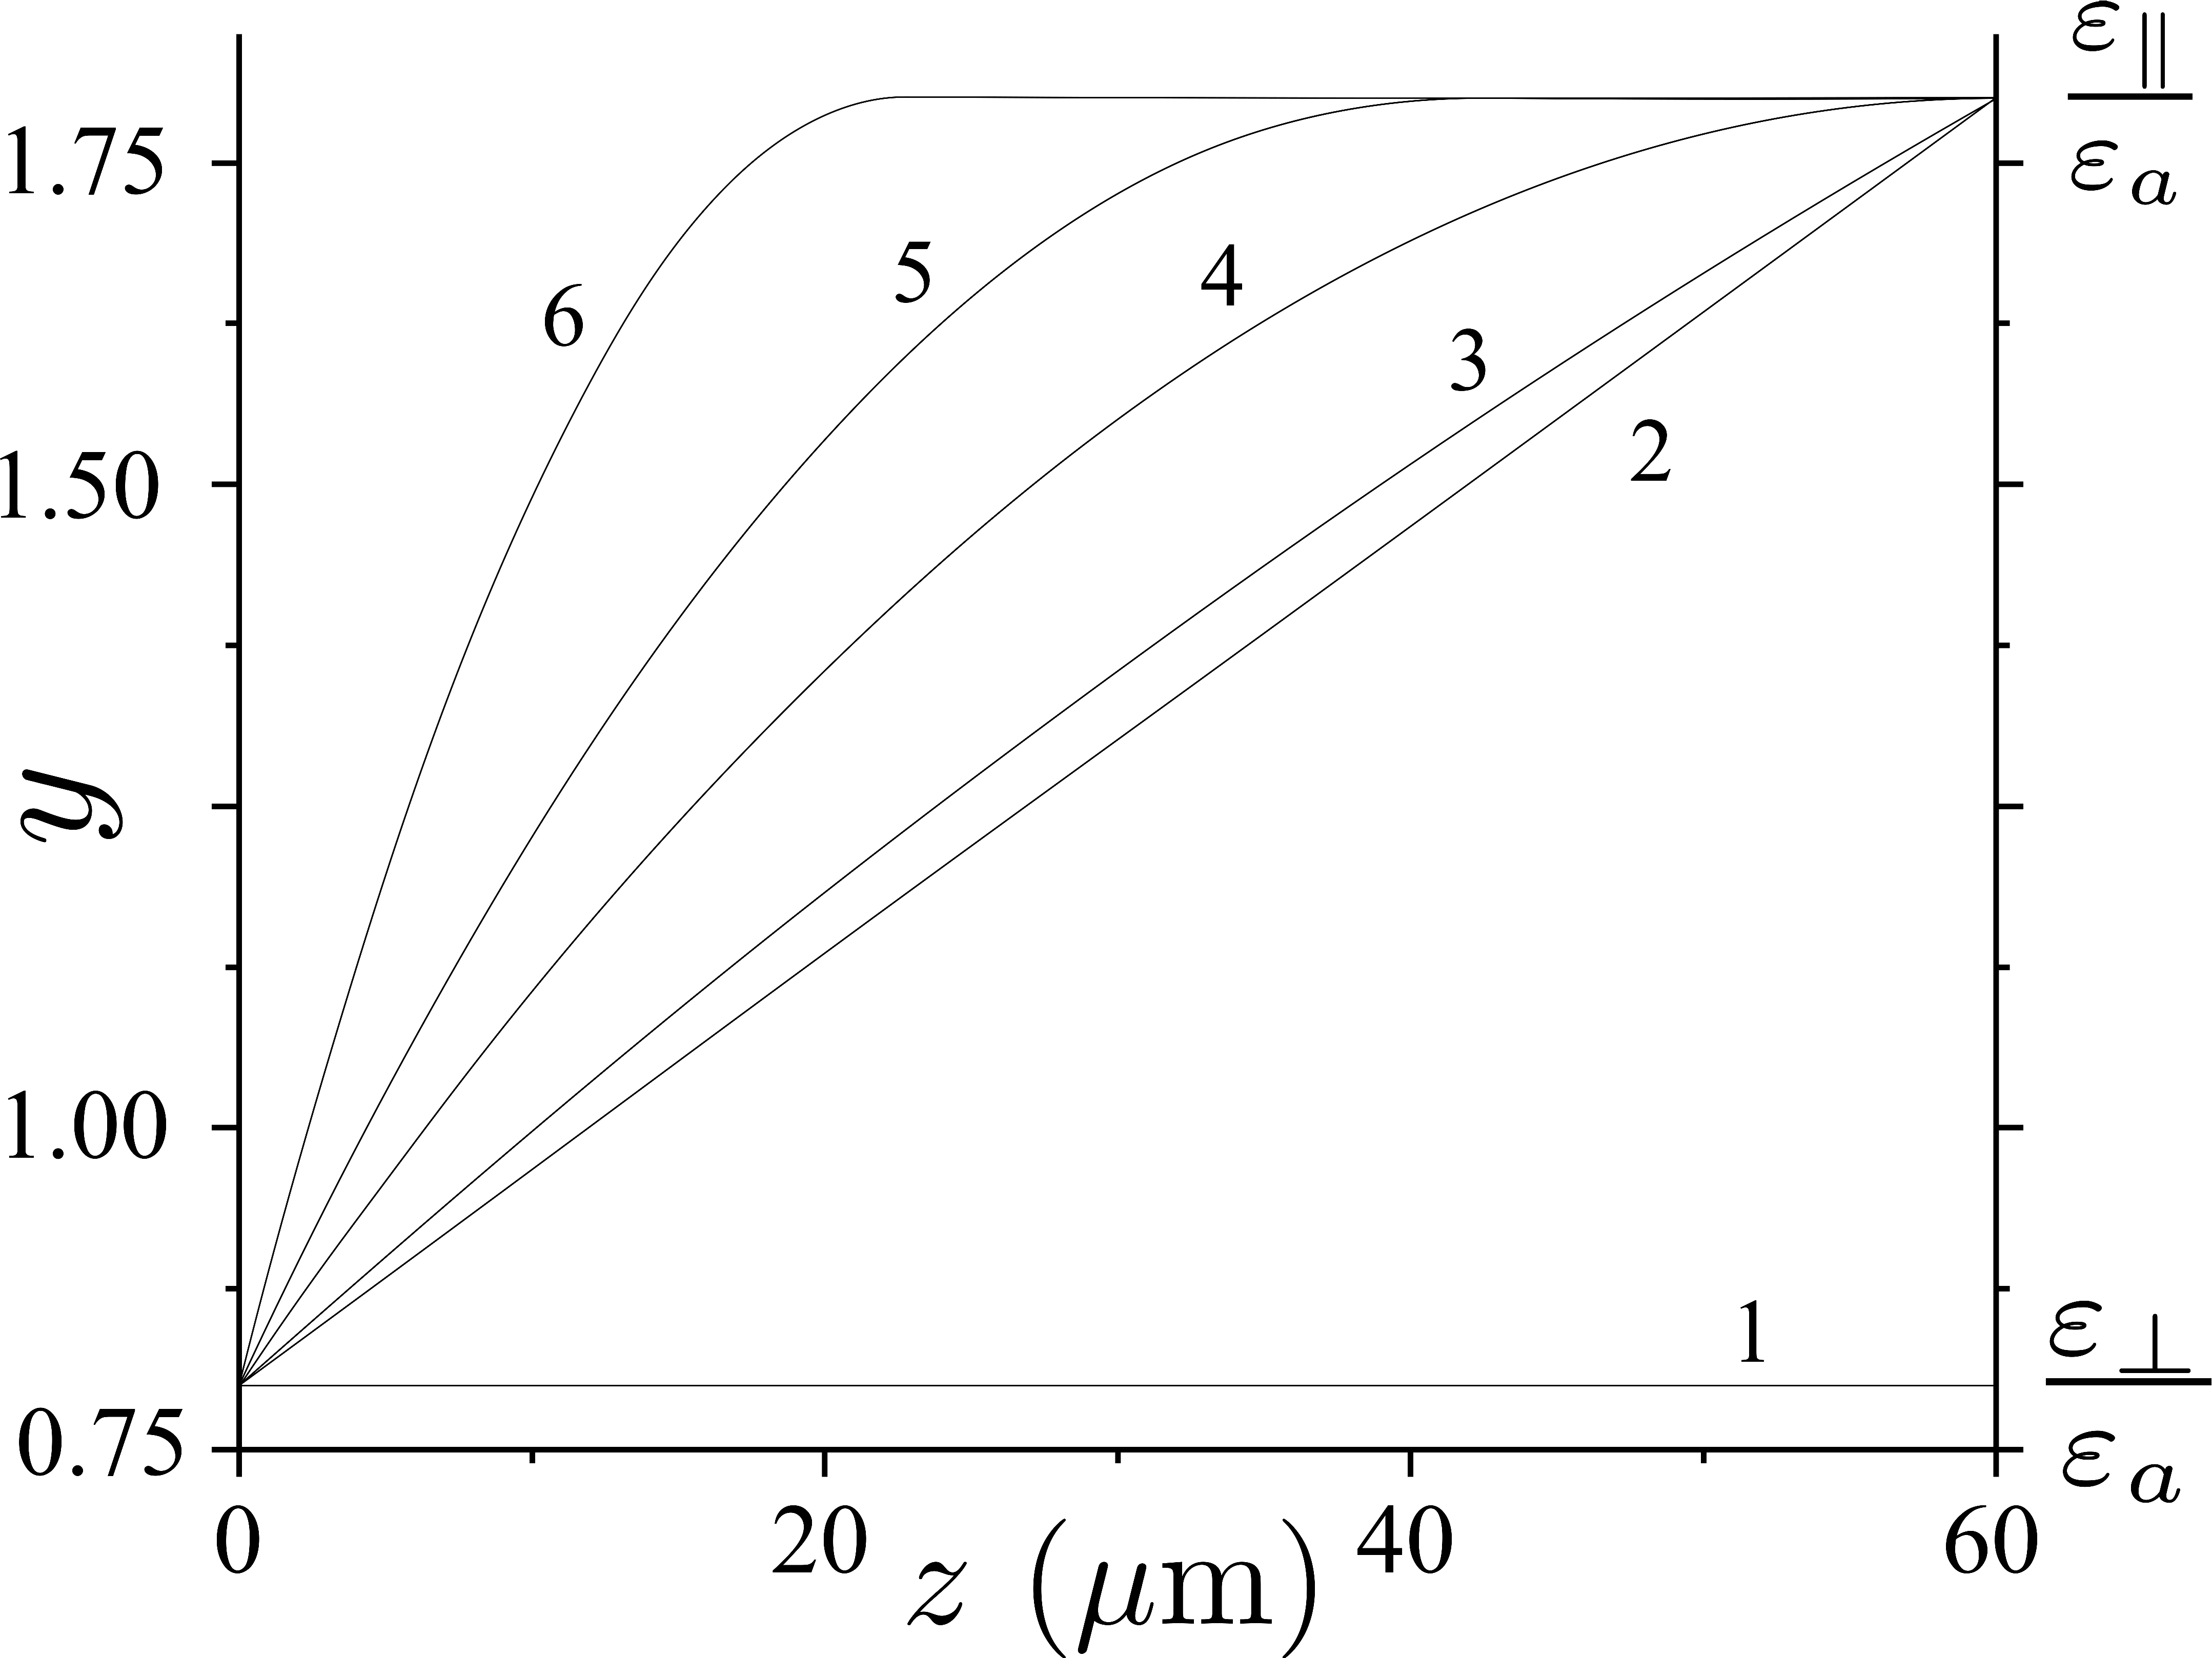
\includegraphics[width=18.8pc]{Fig1_y_low_anchoring.eps}
	\caption{Графики зависимостей $\theta(z)$ (слева) и $y(z)$ (справа), полученные в случае слабого сцепления с правой подложкой, когда выполнено неравенство~\eqref{ineq_g2L_1}.
		Модули сцепления с границами для каждого графика: $W_\theta^{(1)}=0.0025\ \text{эрг}/\text{см}^2$, $W_\theta^{(2)} = 5\times 10^{-4}\ \text{эрг}/\text{см}^2$
		Соответствие линий и приложенного напряжения: 1 -- $U = 0.04$~В, 2 -- $U = 0.05$~В, 3 -- $U = 1.5$~В, 4 -- $U = 4.67$~В, 5 -- $U = 7.5$~В, 6 -- $U = 15$~В.}\label{ch5:fig1}
\end{figure}
Отметим, что кривая $1$ сответствует области малых напряжений $U$, и для неё требование~\eqref{criterion_eU} не выполнено.
Тем не менее, она оказывается близка к зависимости, полученной при помощи численной минимизации полной свободной энергии~\eqref{eq:free-energy}.
Можно также увидеть значительный скачкообразный переход между кривыми $1$ и $2$.
Этот переход происходит при достижении напряжения
\begin{equation}
\widetilde{U}_1 = \frac{8\pi \bar{e}}{\ve_a}\ln{\left( 1 + \frac{g_2 L}{2} \right)}.
\end{equation}
Следует отметить, что для использованных параметров $g_2 L \ll 1$, следовательно, в этом случае $\widetilde{U}_1\simeq W_\theta^{(2)}L/(2\bar{e})$.
С дальнейшим ростом $U$ ориентационная структура меняется без скачков, и при достижении напряжения
\begin{equation}
U_1 = \frac{8\pi \bar{e}}{\ve_a}\ln{\left( \frac{\varkappa + 1}{\varkappa} \right)},
\end{equation}
в объёме ячейки возникает область насыщения, в которой $\theta = 0$, а при увеличении приложенного напряжения эта область увеличивается (см. кривые 5 и 6 на Рис.~\ref{ch5:fig1}).

\todo{``Среднее сцепление''}
В случае, когда константа сцепления с границами удовлетворяет неравенствам
\begin{align}\label{mid_anch}
\frac{2}{\varkappa}< g_2L < \frac{4}{\varkappa - 1},
\end{align}
трансформация ориентационной структуры происходит по другому сценарию, что показано на Рис.~\ref{ch5:fig2}.
\begin{figure}[h]
	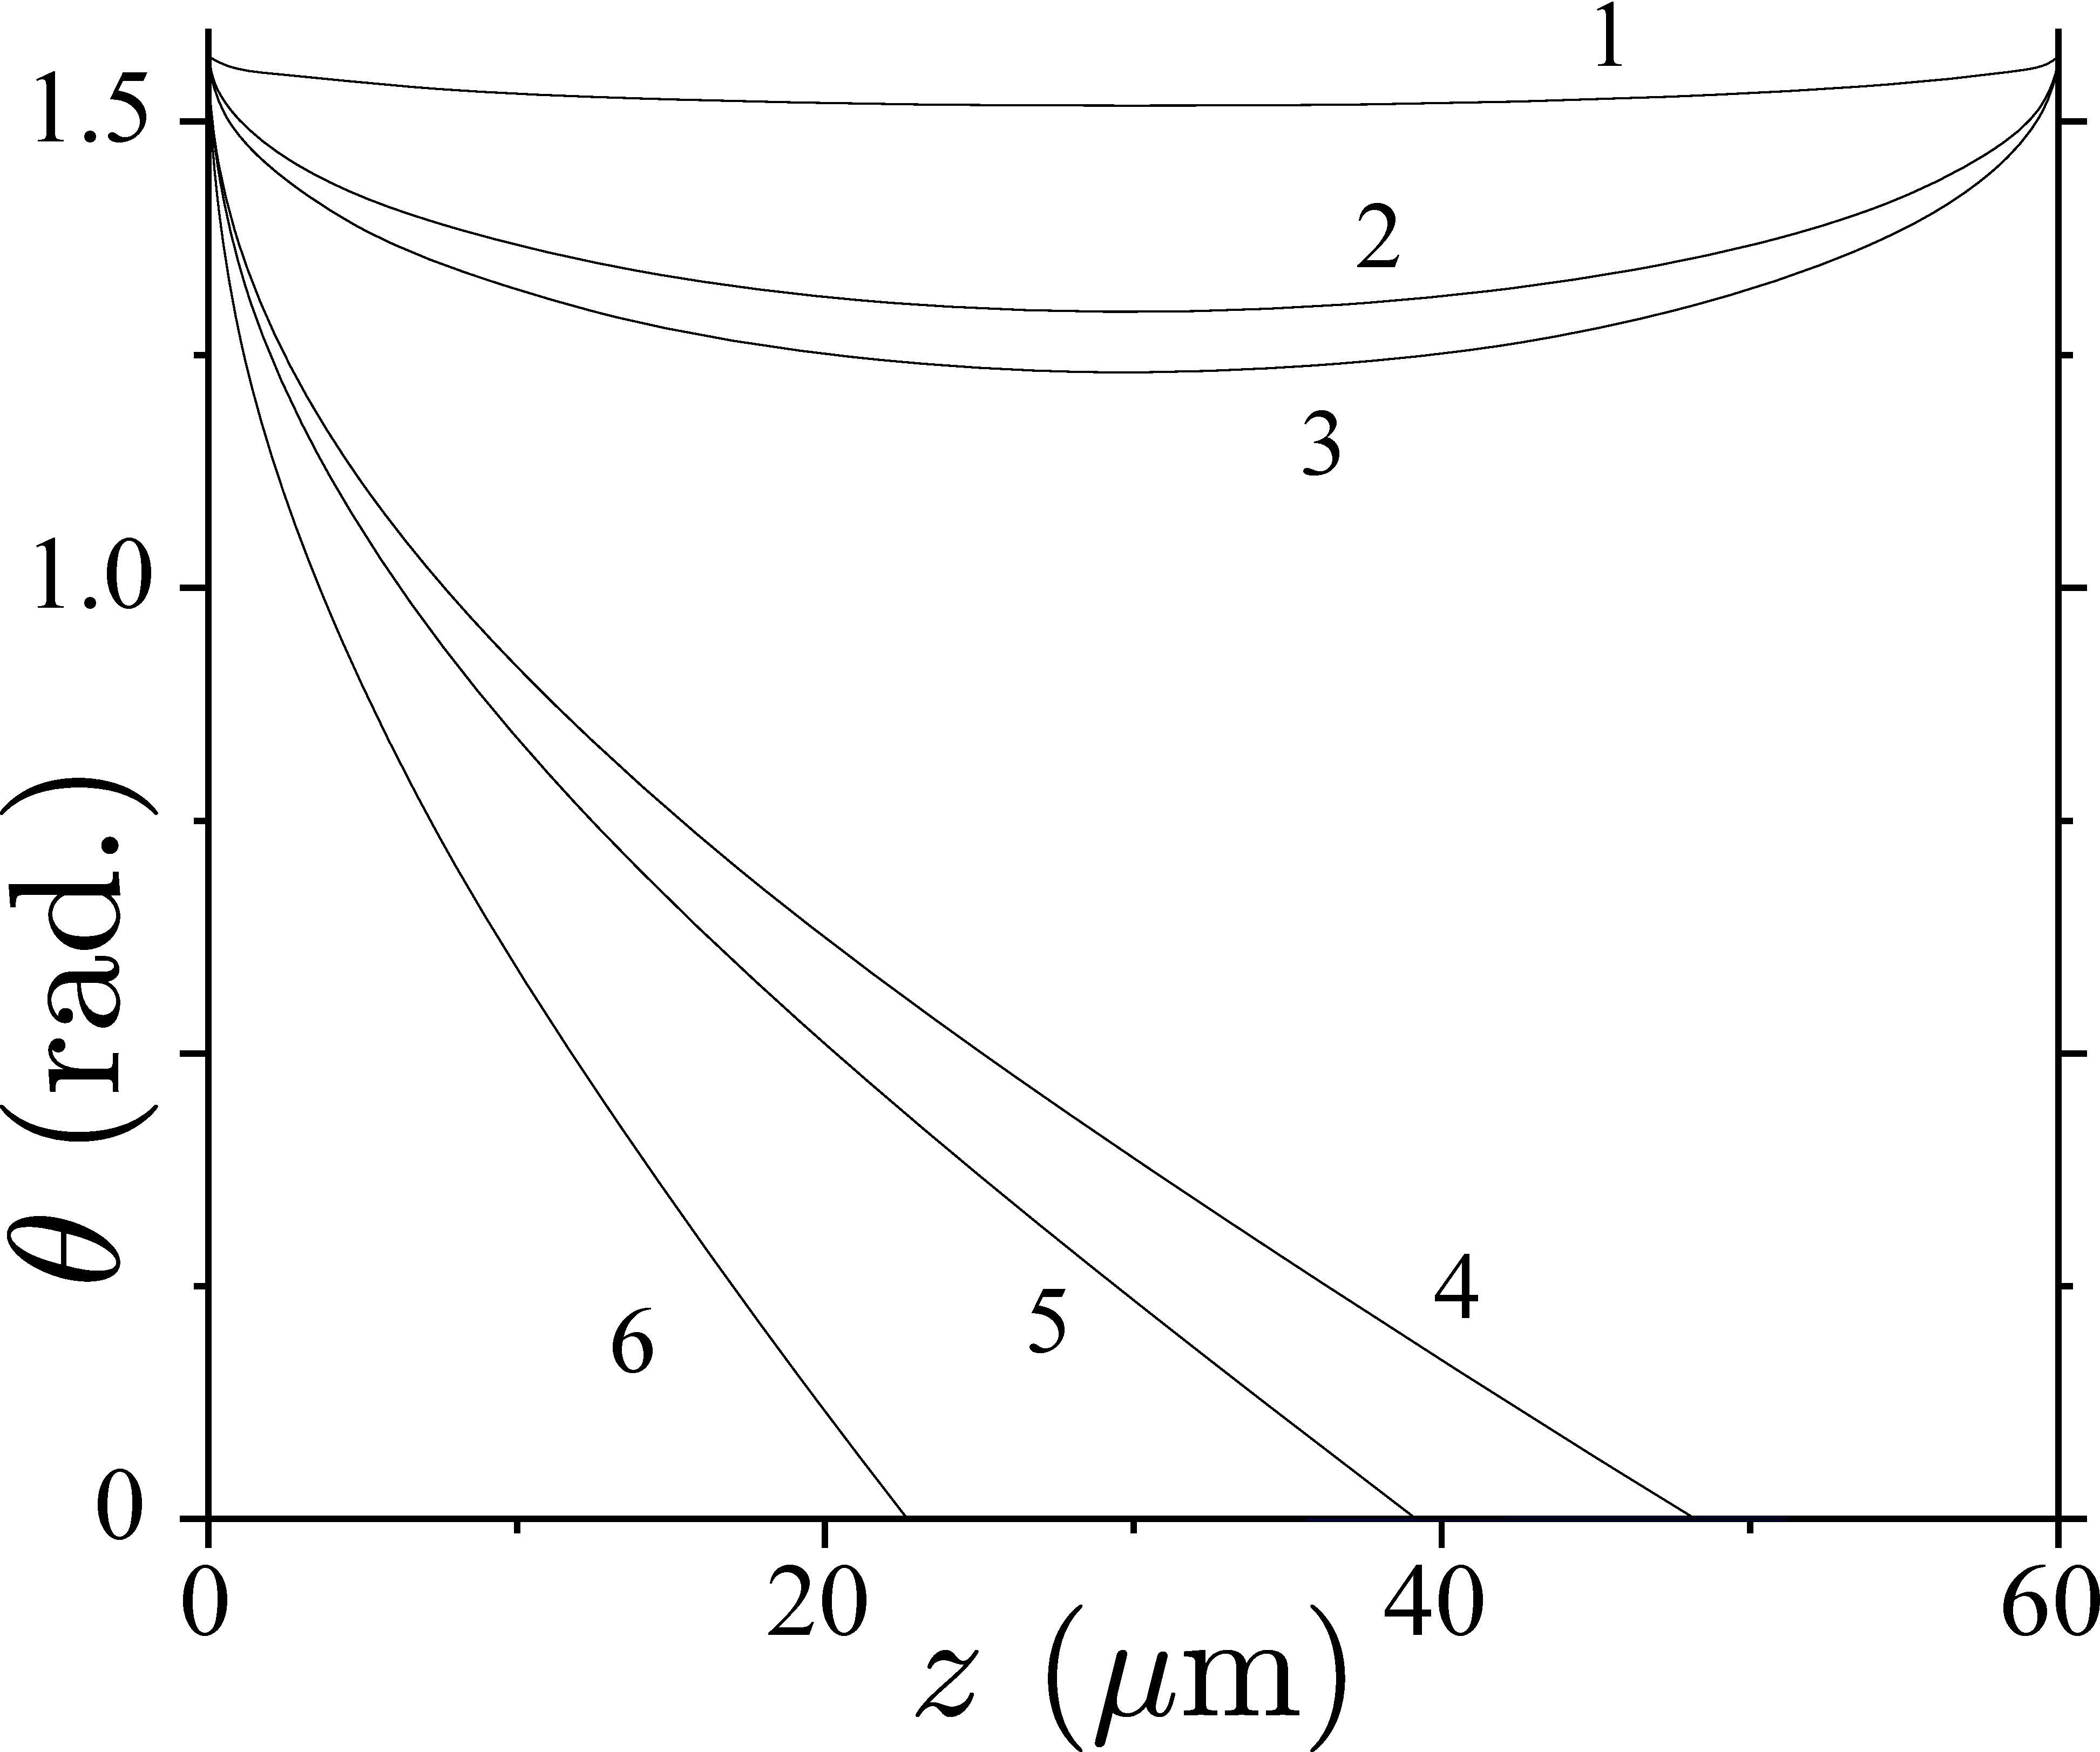
\includegraphics[width=16.9pc]{Fig2_theta_mid_anchoring.eps}\hspace{2pc}%
	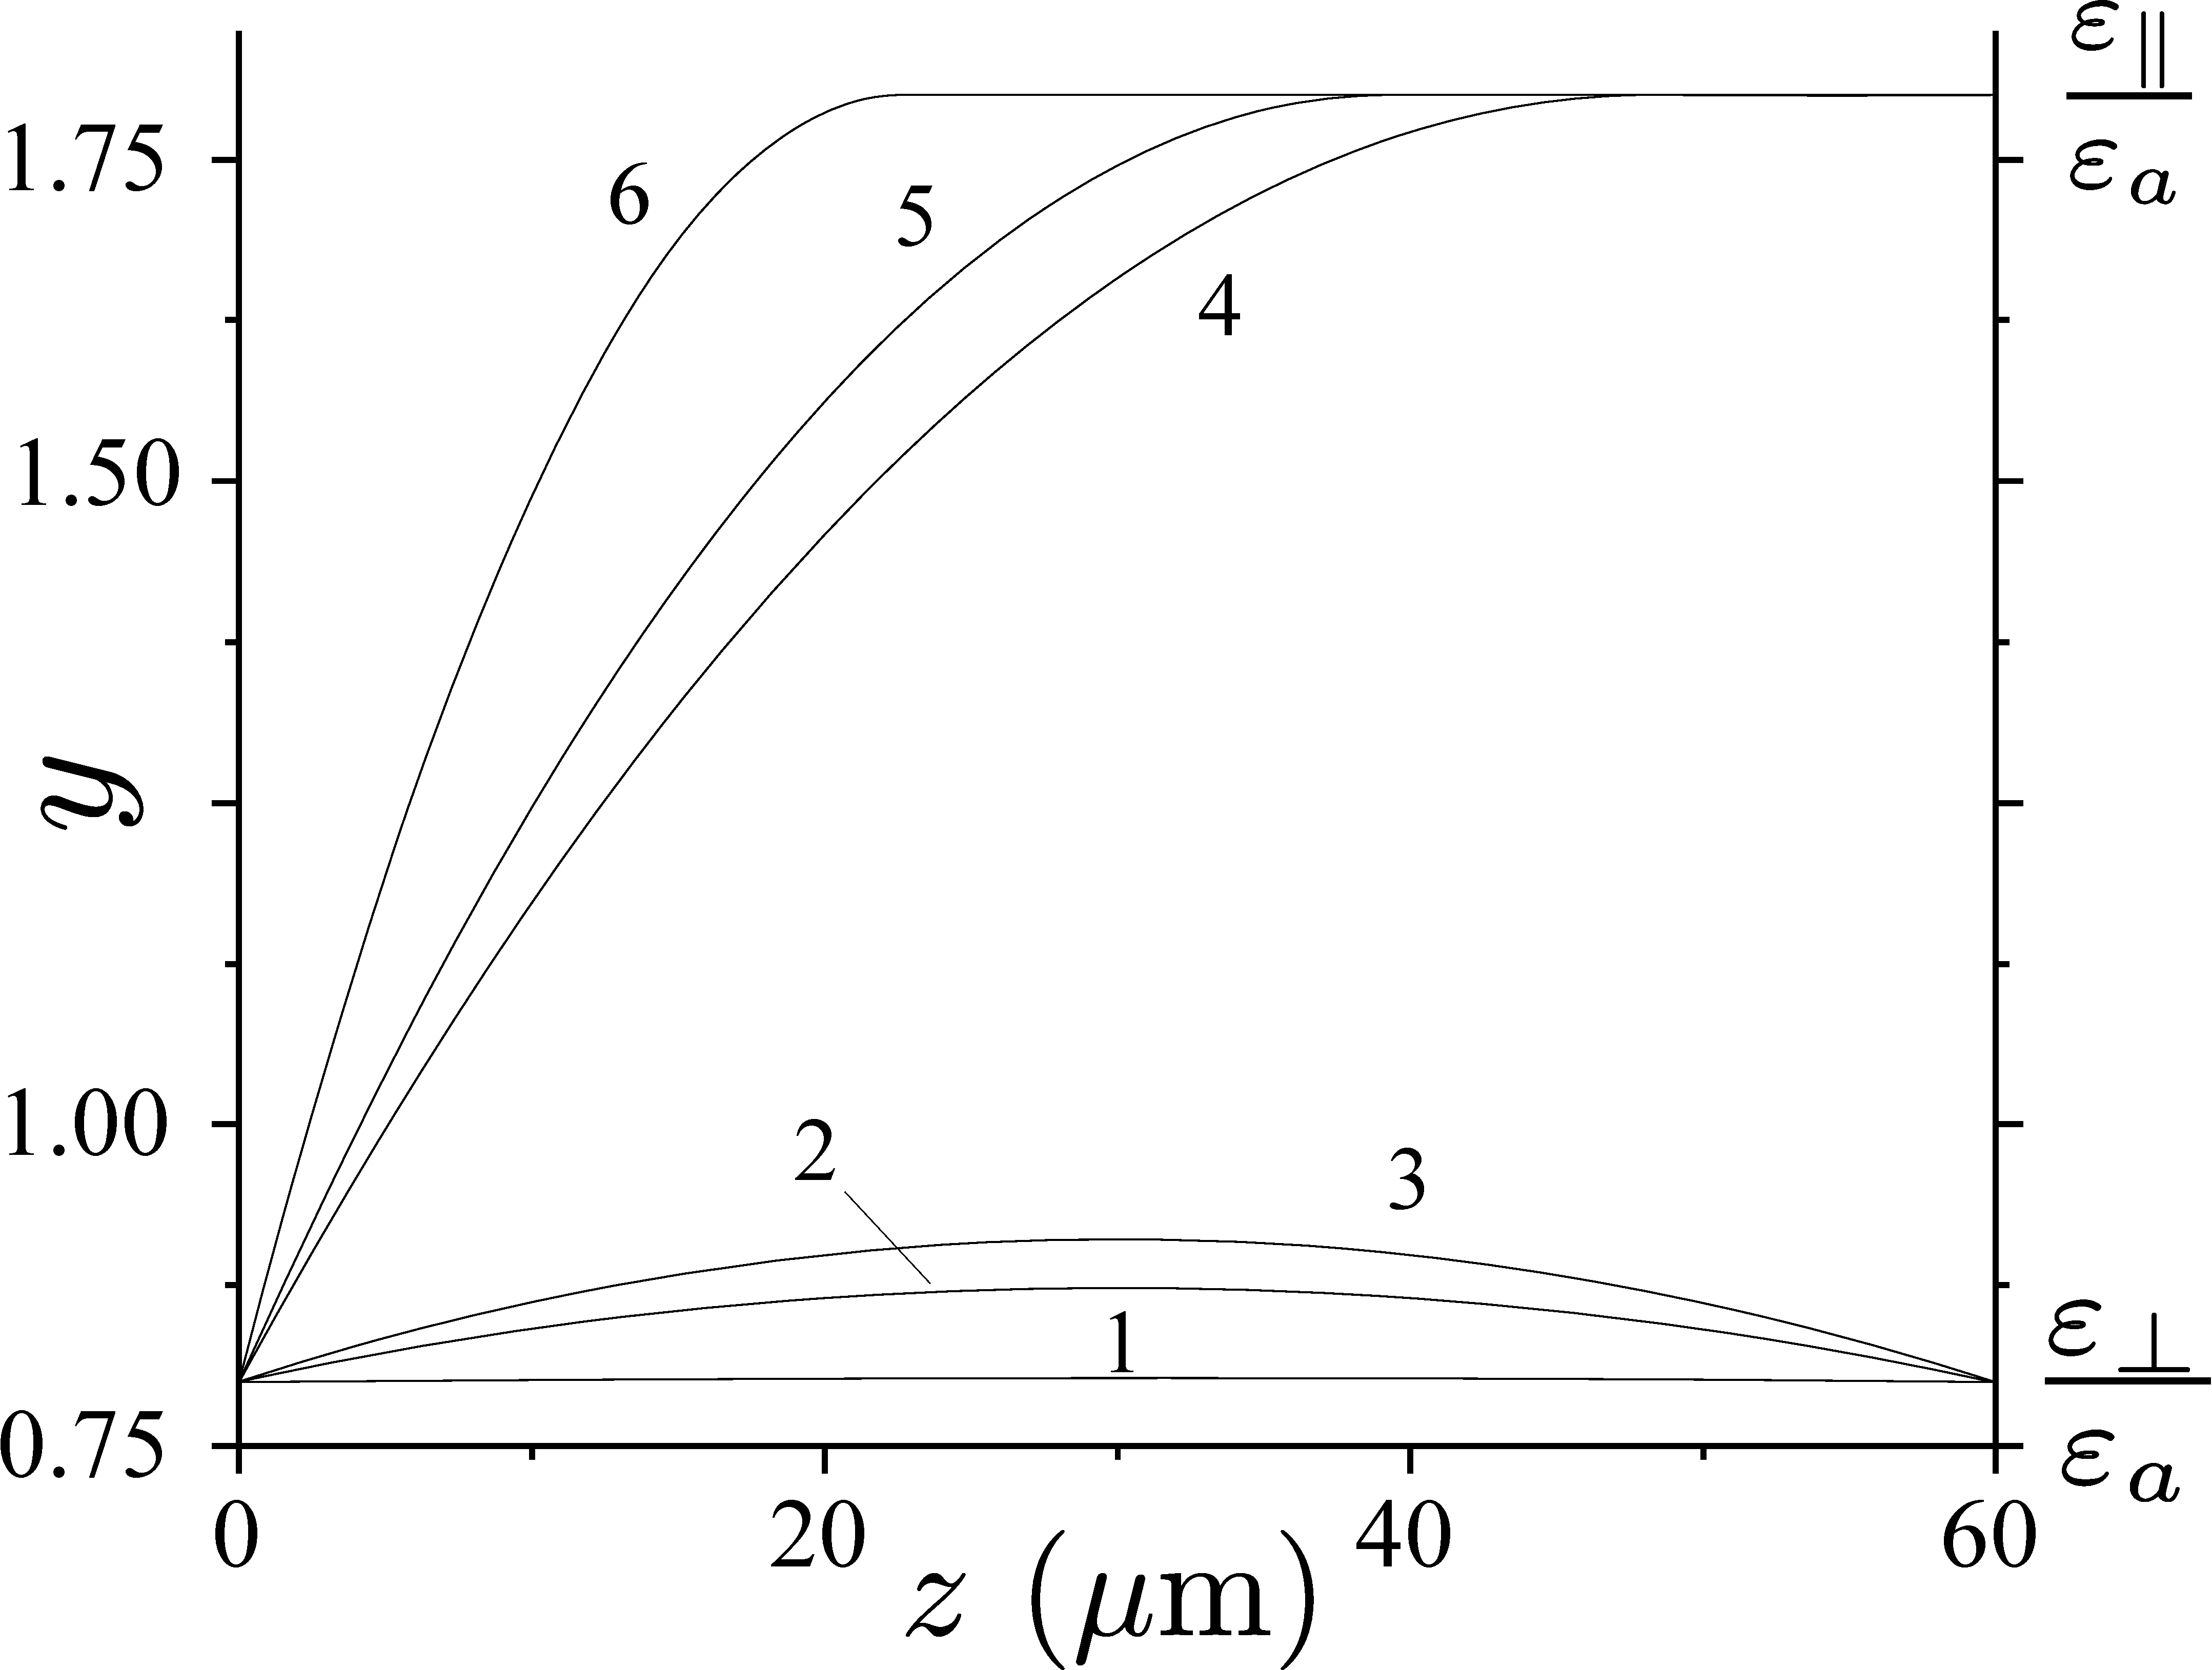
\includegraphics[width=18.9pc]{Fig2_y_mid_anchoring.eps}
	\caption{Графики зависимостей $\theta(z)$ (слева) и $y(z)$ (справа), полученные в случае среднего сцепления с подложкой, когда выполнено неравенство~\eqref{mid_anch}.
		Значения модулей сцепления с подложкой для всех кривых: $W_\theta^{(1)}=0.25\ \text{эрг}/\text{см}^2$, $W_\theta^{(2)} = 0.10\ \text{эрг}/\text{см}^2$.
		Соответствие линий и приложенного напряжения: 1 -- $U = 1$~В, 2 -- $U = 5$~В, 3 -- $U = 6.1$~В, 4 -- $U = 6.2$~В, 5 -- $U = 8$~В, 6 -- $U = 15$~В.}\label{ch5:fig2}
\end{figure}
При этом изменение ориентационной структуры при небольших напряжениях $U$ аналогично происходившим в предыдущем случае, однако когда напряжение достигает значения $\widetilde{U}_1$, происходит скачкообразный переход между кривыми 3 и 4.
Важной особенностью этого случая является то, что область насыщения в объёме ячейки появляется сразу после перехода.
Как и в предыдущем случае, при дальнейшем увеличении напряжения область насыщения в объёме растёт.

\todo{``Сильное зацепление''}

\todo{АО: В описании этого случая ошибка. При отрыве границы она не сразу оказывается насыщенной, и там есть ещё одно характеристическое напряжение}

Наконец, когде энергия сцепления с подложкой удовлетворяет неравенству
\begin{equation}\label{ineq_strong_anch}
g_2L > \frac{4}{\varkappa - 1},
\end{equation}
наблюдается третий сценарий эволюции ориентационной структуры.
\begin{figure}[ht]
	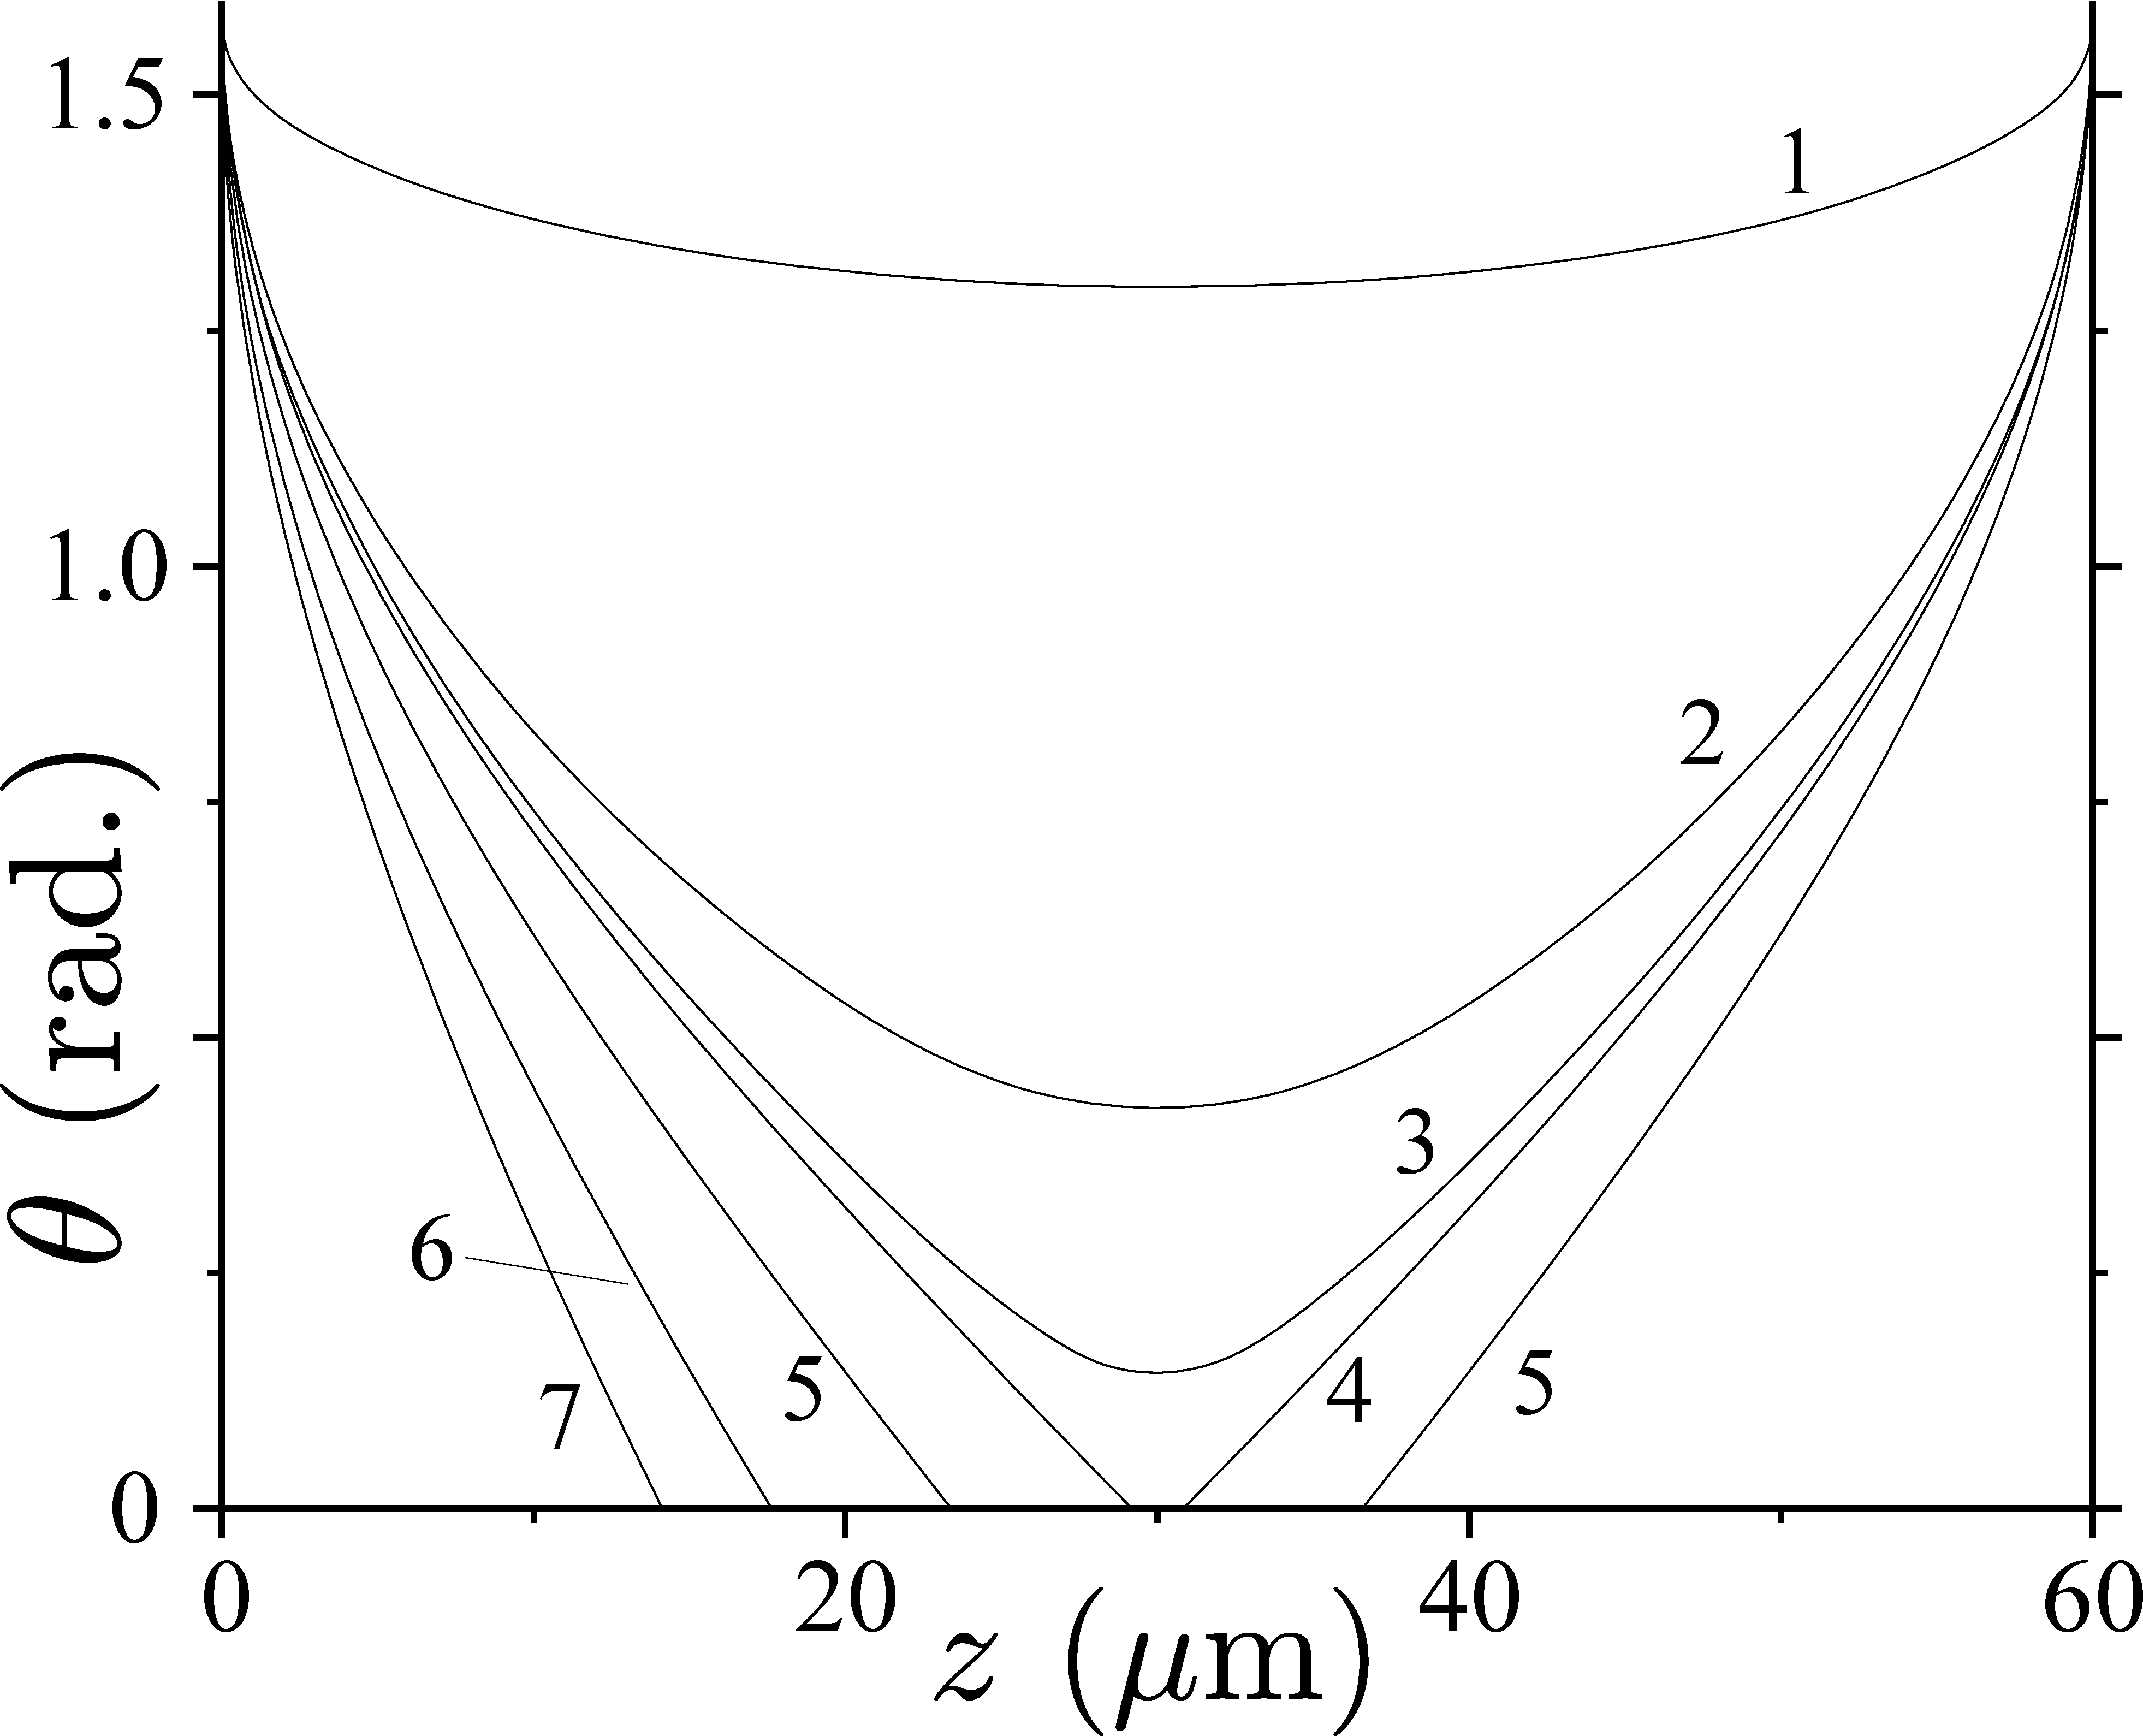
\includegraphics[width=17pc]{Fig3_theta_high_anchoring.eps}\hspace{2pc}%
	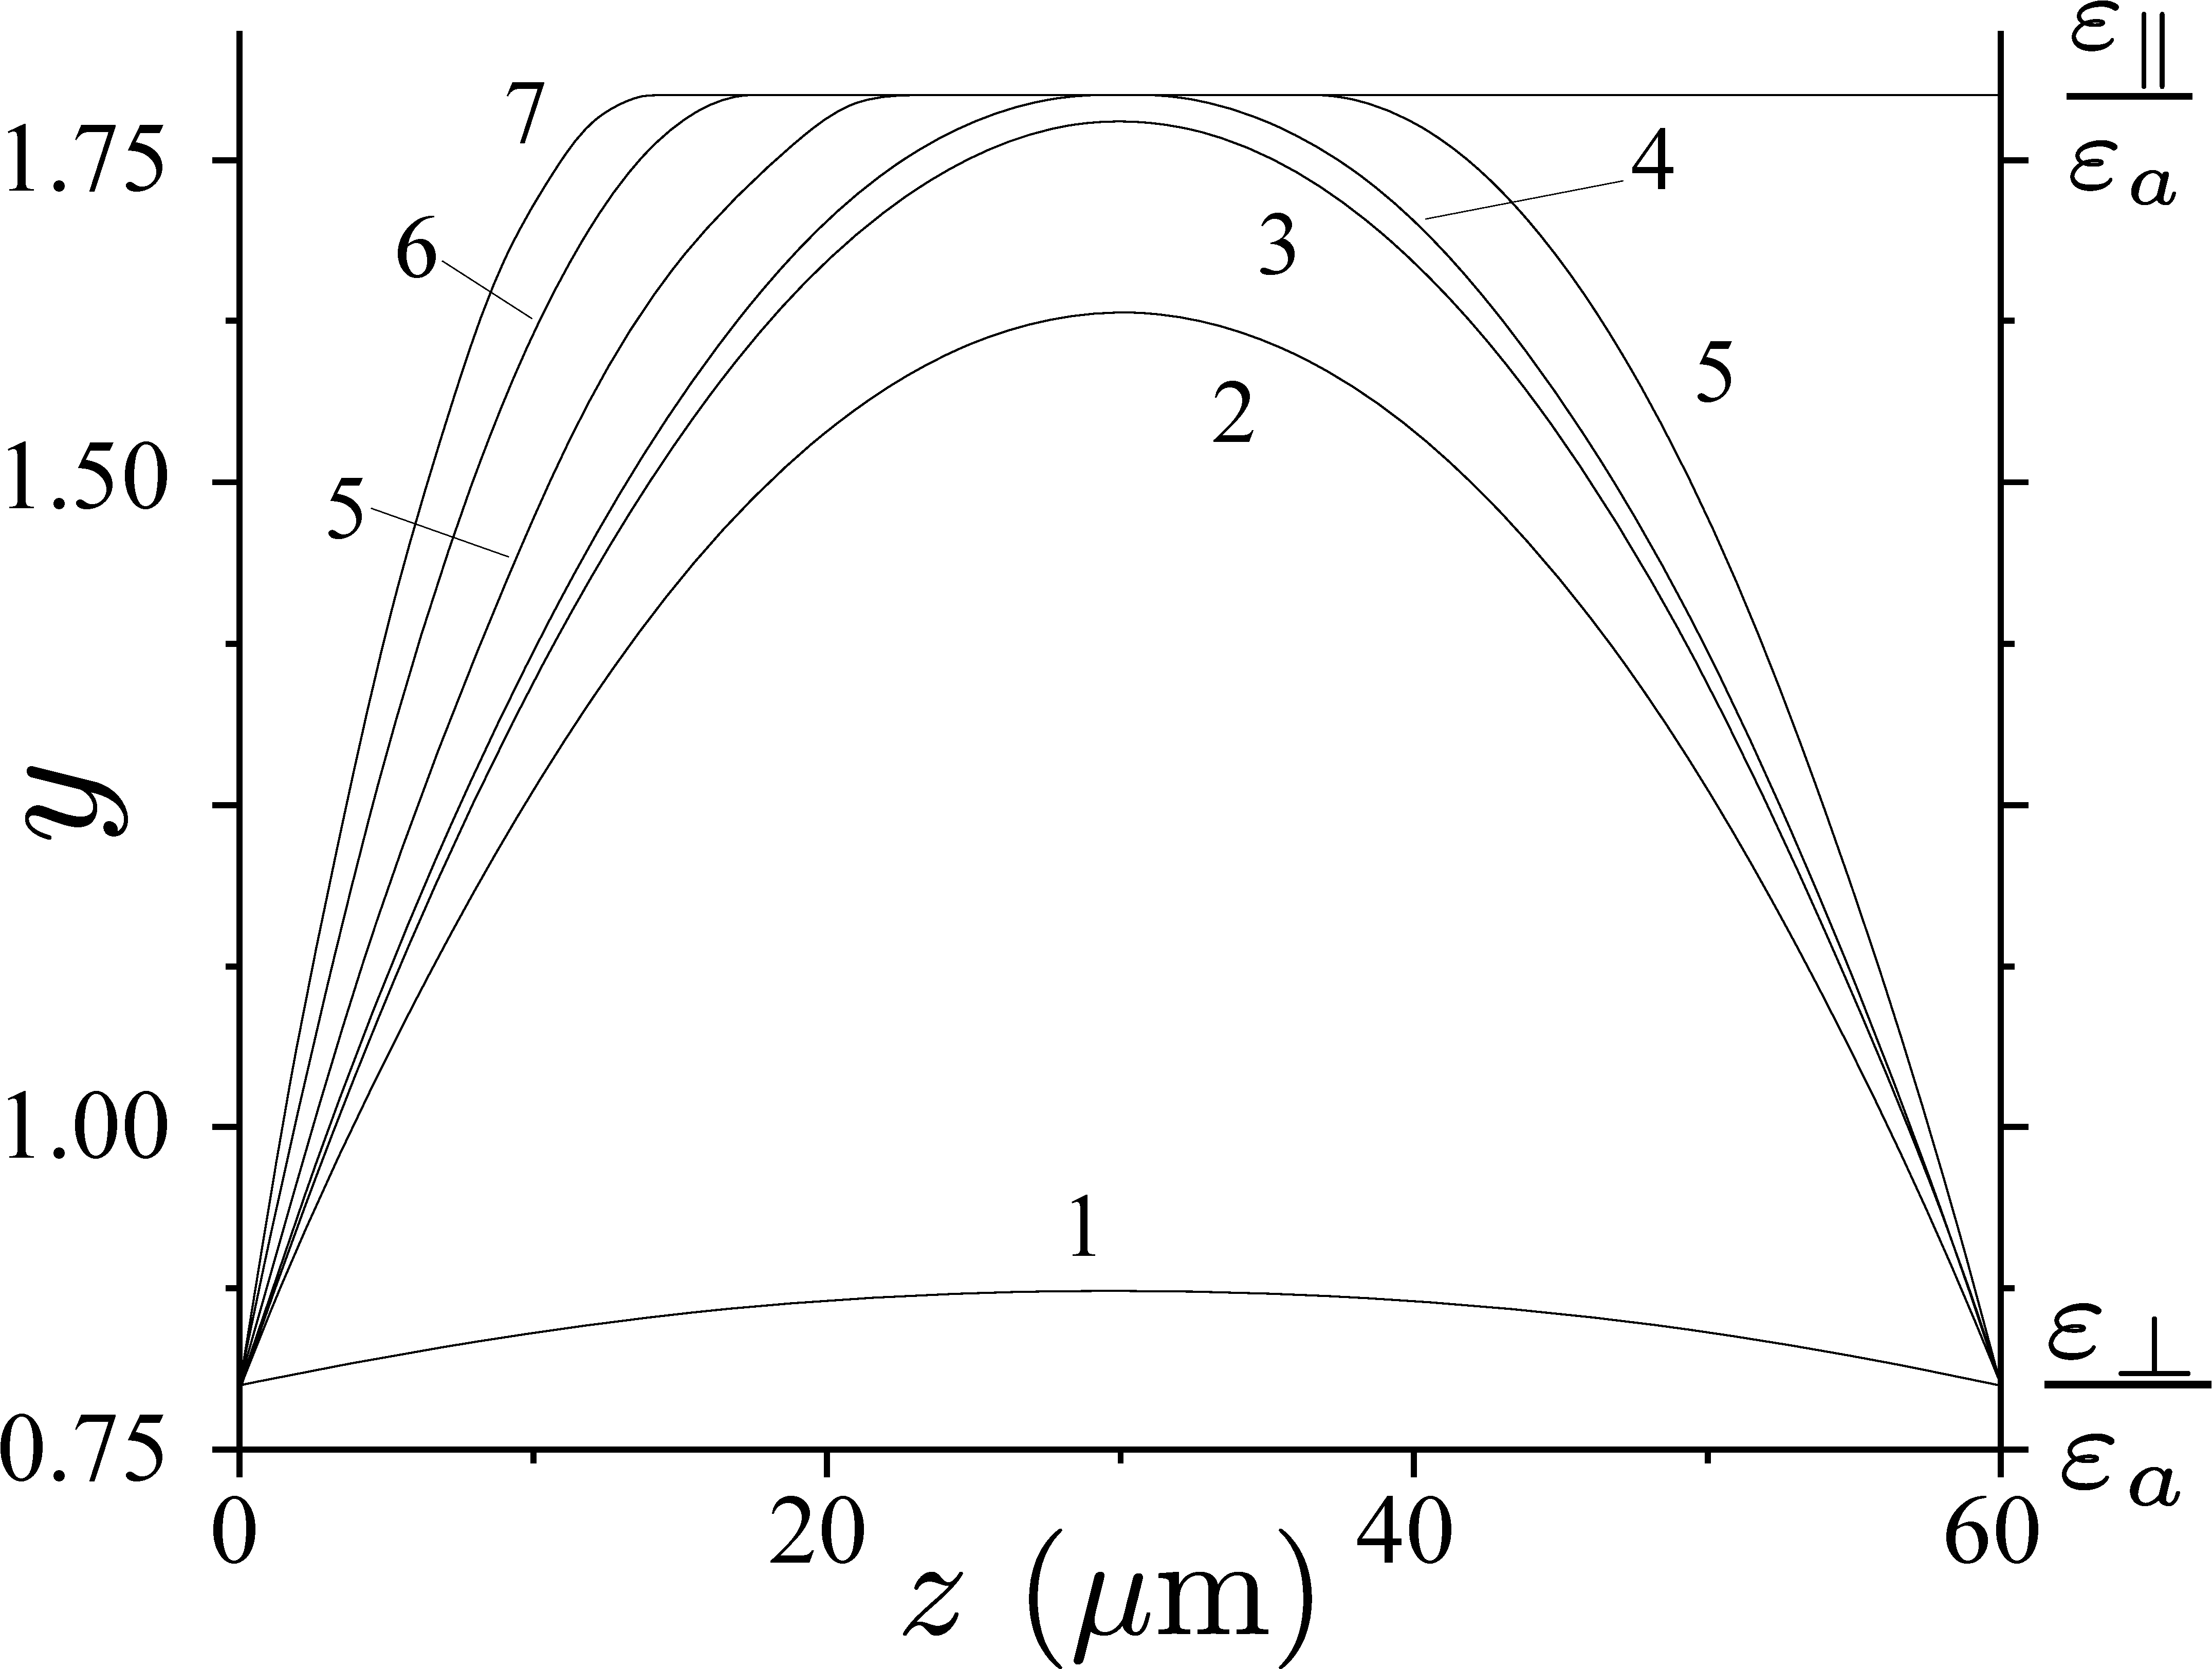
\includegraphics[width=18.9pc]{Fig3_y_high_anchoring.eps}
	\caption{Графики зависимостей $\theta(z)$ (слева) и $y(z)$ (справа), полученные для случая сильного сцепления с подложкой, когда выполнено неравенство~\eqref{ineq_strong_anch}.
		Модули сцепления с подложкой для всех кривых: $W_\theta^{(1)}=1.75\ \text{эрг}/\text{см}^2$, $W_\theta^{(2)} = 0.7\ \text{эрг}/\text{см}^2$.
		Соответствие линий и приложенного напряжения: 1 -- $U = 5$~В, 2 -- $U = 15$~В, 3 -- $U = 16$~В, 4 -- $U = 16.5$~В, 5 -- $U = 19.65$~В, 6 -- $U = 19.75$~В, 7 -- $U = 25$~В.}\label{ch5:fig3}
\end{figure}
Этот сценарий показан на Рис.~\ref{ch5:fig3}.
Опять же, трансформации при малых напряжениях $U$ аналогичны предыдущим случаям.
Однако когда напряжение достигает значения
\begin{equation}
U_2 = \frac{8\pi\bar{e}}{\ve_a}\ln\left( \frac{\varkappa + 1}{\varkappa - 1} \right),
\end{equation} 
в середине ячейки появляется область насыщения (кривые 4 и 5 на Рис.~\ref{ch5:fig3}).
С ростом $U$ эта область продолжает симметрично расширяться от центра ячейки до тех пор, пока напряжение не достигнет значения
\begin{equation}
\widetilde{U}_2 = U_2 + \frac{8\pi \bar{e}}{\ve_a}\left(\frac{g_2L}{2}\cdot\frac{\varkappa}{\varkappa - 1}\cdot \frac{\ve_\bot}{\ve_\parallel} - \frac{2}{\varkappa}\right).
\end{equation}
Когда это происходит, ориентационная структура скачком меняется от описываемой линией 5 на Рис.~\ref{ch5:fig3} до описываемой кривой 6 (при указанном наборе параметров пороговое напряжение составляет $U_2 = 19.68$~В).
Интересно, что если сравнить графики 5 и 6, можно увидеть, что в результате переходе область насыщения расширилась и справа, и слева от центра.
При дальнейшем увеличении $U$ область насыщения также увеличивается (см. линии 6 и 7 на Рис.~\ref{ch5:fig3}).

полученные результаты показывают, что в ячейках с большим усреднённым флексоэлектрическим коэффициентом возможны три сценария эволюции ориентационной структуры с ростом приложенного напряжения.
При этом то, какой сценарий будет реализовываться, зависит от энергии сцепления с одной из границ.
Наши результаты также показали, что в таких ЖК-ячейках возможны разнообразные скачкообразные ориентационные переходы, а также переходы к насыщению.
Такие свойства могут быть использованы при разработке переключателей нового типа.           % Глава 5
%\chapter*{Заключение}                       % Заголовок
\addcontentsline{toc}{chapter}{Заключение}  % Добавляем его в оглавление

%% Согласно ГОСТ Р 7.0.11-2011:
%% 5.3.3 В заключении диссертации излагают итоги выполненного исследования, рекомендации, перспективы дальнейшей разработки темы.
%% 9.2.3 В заключении автореферата диссертации излагают итоги данного исследования, рекомендации и перспективы дальнейшей разработки темы.
%% Поэтому имеет смысл сделать эту часть общей и загрузить из одного файла в автореферат и в диссертацию:

Основные результаты работы заключаются в следующем.
%% Согласно ГОСТ Р 7.0.11-2011:
%% 5.3.3 В заключении диссертации излагают итоги выполненного исследования, рекомендации, перспективы дальнейшей разработки темы.
%% 9.2.3 В заключении автореферата диссертации излагают итоги данного исследования, рекомендации и перспективы дальнейшей разработки темы.
\begin{enumerate}
  \item На основе анализа \ldots
  \item Численные исследования показали, что \ldots
  \item Математическое моделирование показало \ldots
  \item Для выполнения поставленных задач был создан \ldots
\end{enumerate}

И какая-нибудь заключающая фраза.

Последний параграф может включать благодарности.       % Заключение
%\chapter*{Список сокращений и условных обозначений} % Заголовок
\addcontentsline{toc}{chapter}{Список сокращений и условных обозначений}  % Добавляем его в оглавление
\noindent
%\begin{longtabu} to \dimexpr \textwidth-5\tabcolsep {r X}
\begin{longtabu} to \textwidth {r X}
% Жирное начертание для математических символов может иметь
% дополнительный смысл, поэтому они приводятся как в тексте
% диссертации
\({\boldsymbol{\hat{\mathrm e}}}\) & единичный вектор \\
\(E_0\) & амплитуда падающего поля\\

\end{longtabu}
\addtocounter{table}{-1}% Нужно откатить на единицу счетчик номеров таблиц, так как предыдующая таблица сделана для удобства представления информации по ГОСТ
        % Список сокращений и условных обозначений
%\chapter*{Словарь терминов}             % Заголовок
\addcontentsline{toc}{chapter}{Словарь терминов}  % Добавляем его в оглавление

\textbf{TeX} : Cистема компьютерной вёрстки, разработанная американским профессором информатики Дональдом Кнутом

\textbf{панграмма} : Короткий текст, использующий все или почти все буквы алфавита
      % Словарь терминов
\clearpage                                  % В том числе гарантирует, что список литературы в оглавлении будет с правильным номером страницы
%\hypersetup{ urlcolor=black }               % Ссылки делаем чёрными
%\providecommand*{\BibDash}{}                % В стилях ugost2008 отключаем использование тире как разделителя
\urlstyle{rm}                               % ссылки URL обычным шрифтом
\ifdefmacro{\microtypesetup}{\microtypesetup{protrusion=false}}{} % не рекомендуется применять пакет микротипографики к автоматически генерируемому списку литературы
\insertbibliofull                           % Подключаем Bib-базы
\ifdefmacro{\microtypesetup}{\microtypesetup{protrusion=true}}{}
\urlstyle{tt}                               % возвращаем установки шрифта ссылок URL
%\hypersetup{ urlcolor={urlcolor} }          % Восстанавливаем цвет ссылок      % Список литературы
%\clearpage
\ifdefmacro{\microtypesetup}{\microtypesetup{protrusion=false}}{} % не рекомендуется применять пакет микротипографики к автоматически генерируемым спискам
\listoffigures  % Список изображений

%%% Список таблиц %%%
% (ГОСТ Р 7.0.11-2011, 5.3.10)
\clearpage
\listoftables   % Список таблиц
\ifdefmacro{\microtypesetup}{\microtypesetup{protrusion=true}}{}
\newpage           % Списки таблиц и изображений (иллюстративный материал)

%%% Настройки для приложений
\appendix
% Оформление заголовков приложений ближе к ГОСТ:
\setlength{\midchapskip}{20pt}
\renewcommand*{\afterchapternum}{\par\nobreak\vskip \midchapskip}
\renewcommand\thechapter{\Asbuk{chapter}} % Чтобы приложения русскими буквами нумеровались

%\chapter{Примеры вставки листингов программного кода}\label{app:A}

Для крупных листингов есть два способа. Первый красивый, но в нём могут быть
проблемы с поддержкой кириллицы (у вас может встречаться в~комментариях
и печатаемых сообщениях)        % Приложения

\end{document}
